\documentclass{report}
\usepackage[utf8]{inputenc}
\usepackage[T1]{fontenc}
\usepackage[french]{babel}
\usepackage{lmodern}
\usepackage{amsmath}
\usepackage{amssymb}
\usepackage{amsthm}
\usepackage{dsfont}
\usepackage{caption}
\usepackage{algorithm}
\usepackage{algpseudocode}
\usepackage{array}
\usepackage{pgf,tikz}
\usepackage{subfig}
\usepackage{verbatim}
\usetikzlibrary{arrows}
\usepackage{pgf,tikz}
\usepackage{hyperref}
\usepackage[justification=centering]{caption}
\usepackage{adjustbox}   

\theoremstyle{plain}
\newtheorem{proposition}{Proposition}
\newtheorem{theorem}{Théorème}
\newtheorem{lemma}{Lemme}
\newtheorem{corollary}{Corollaire}


\theoremstyle{definition}
\newtheorem{definition}{Définition}
\newtheorem{conjecture}{Conjecture}

\theoremstyle{remark}
\newtheorem{remark}{Remarque}
\newtheorem{example}{Exemple}
	
\title{Compte-rendu}
\author{Vincent \textsc{Auriau} -- Laurent \textsc{Beaughon} -- Marc \textsc{Belicard} \\ Yaqine \textsc{Hechaichi} -- Thaïs \textsc{Rahoul} -- Pierre \textsc{Vigier}}

\begin{document}

\maketitle

\tableofcontents

\chapter{Réseaux de neurones}

\section{Apprentissage automatique}

Avant de parler de neurones et de réseaux de neurones, nous commencerons par rappeler rapidement ce qu'est l'apprentissage automatique, ses différentes formes et fixerons certaines notations pour la suite de ce document.

L'apprentissage automatique au sens général peut être défini comme un processus permettant à une machine d'évoluer afin de résoudre une tâche ou un problème. Il en existe plusieurs formes parmi lesquelles l'apprentissage supervisé, l'apprentissage non-supervisé et l'apprentissage par renforcement.

L'apprentissage supervisé est celui qui nous intéressera le plus, il sera donc davantage détaillé. Dans un problème d'apprentissage il est donné un ensemble de taille finie $N$ de couples d'entrée, sortie que nous noterons $(x^{(1)},y^{(1)}), ..., (x^{(N)}, y^{(N)})$. Ces couples sont appelés exemples. Les entrées proviennent d'un espace $\mathcal{X}$ de dimension $n$ et les sorties d'un espace $\mathcal{Y}$ de dimension $m$. Une hypothèse classique de l'apprentissage automatique est de supposer que les entrées sont générées de manière indépendante selon une certaine loi de probabilité sur $\mathcal{X}$. Plus formellement, les $(x^{(i)})_{i \in \{1, ..., N\}}$ sont les réalisations de variables aléatoires $(X_i)_{i \in \{1, ..., N\}}$ avec les $X_i$ indépendantes et identiquement distribuées selon une probabilité $p$. Pour plus de commodités, notons $X = \{x^{(i)}, \forall i \in \{1, ..., N\}\}$ et $Y = \{y^{(i)}, \forall i \in \{1, ..., N\}\}$.

L'objectif de l'apprentissage supervisé est alors de découvrir le processus générateur des sorties à partir des entrées. Si ce processus est déterministe, il s'agira d'une fonction $f$ générant les sorties à partir des entrées. L'objectif de l'apprentissage sera donc de trouver à partir des exemples un modèle $\hat{f}$ proche de f. Si le processus est non déterministe, il s'agira alors de retrouver la loi de $p(y|x)$.

Si les sorties prennent leurs valeurs dans un espace $\mathcal{Y}$ infini, le problème est dit de régression. Dans le cas contraire, on parle de problème de classification. Par convention, on choisit les valeurs des classes telles que $\mathcal{Y} = \{0, ..., M-1\}$ avec $M$ le nombre de classes. Si $M = 2$, il s'agit de classification binaire.

Quelque soit le type de problème à résoudre, l'objectif est toujours de trouver une fonction ou une distribution de probabilité proche de celle générant les sorties. Cependant, cette notion de "proche" est très relative. 

\begin{definition}[Erreur sur un exemple]
Soit $e : \mathbb{R}^m \times \mathbb{R}^m \rightarrow \mathbb{R}$ la mesure de performance sur un exemple.
\end{definition}
$e(y, \hat{f}(x))$ représentera l'écart de notre modèle avec la sortie attendue. 

\begin{example}[Erreur quadratique]
Une mesure courante est l'erreur quadratique $e(x, y) \mapsto \Vert x - y \Vert_2^2$.
\end{example}

On définit alors l'erreur sur l'ensemble des exemples :

\begin{definition}[Erreur empirique]
$$
E_{in} = \frac{1}{N}\sum_{i=1}^{N}{e(y^{(i)}, f(x^{(i)})} = \mathbb{E}_{x, y \sim \hat{p}_{data}}(e(y, f(x)))
$$
avec $\hat{p}_{data}$ est la distribution empirique dans l'ensemble des exemples.
\end{definition}

Et l'erreur dans l'absolue, sur toutes les valeurs possibles :

\begin{definition}[Erreur absolue]
$$
E_{out} = \mathbb{E}_{x, y \sim p}(e(y, f(x)))
$$
avec $p$ la distribution réelle des entrées et des sorties.
\end{definition}

L'objectif d'être proche peut alors se traduire par la minimisation de $E_{out}$. Or l'estimation de $E_{out}$ nécessite de connaître $p(x, y)$ pour tout $(x, y)$ dans $\mathcal{X} \times \mathcal{Y}$, ce qui est généralement impossible. Cependant, il est aisé de calculer $E_{in}$, qui est une estimation de $E_{out}$ sur les données disponibles. 

En effet, on a la proposition suivante :
\begin{proposition}
$E_{in}$ est un estimateur non biaisé de $E_{out}$.
\end{proposition}

\begin{proof}
$$
\mathbb{E}_{(x_1, y_1),..., (x_N, y_N) \sim p}(E_{in}) = \frac{1}{N}\sum_{i=1}^{N}{\mathbb{E}_{(x_i, y_i) \sim p}(e(y^{(i)}, f(x^{(i)}))} = \mathbb{E}_{x, y \sim p}(e(y, f(x)))
$$
\end{proof}

Malheureusement, les exemples servant à calculer $E_{in}$ seraient les mêmes que ceux utilisés pour choisir notre modèle. Par conséquent, le modèle serait choisi pour bien fonctionner sur ces exemples. $E_{in}$ sous-estimerait la valeur réelle de $E_{out}$ et ne serait plus un bon proxy pour $E_{out}$.

Une solution simple pour régler ce problème est de découper nos exemples en deux ensembles distincts : l'ensemble d'apprentissage et l'ensemble de test que nous noterons respectivement $(X_{train}, Y_{train})$ et $(X_{test}, Y_{test})$. Nous aurons alors :

\begin{equation}
E_{train} = \frac{1}{N_{train}}\sum_{i=1}^{N_{train}}{e(y^{(i)}_{train}, f(x^{(i)}_{train}))}
\end{equation}

qui servira pour entraîner le modèle pendant l'étape d'apprentissage et :

\begin{equation}
E_{test} = \frac{1}{N_{test}}\sum_{i=1}^{N_{test}}{e(y^{(i)}_{test}, f(x^{(i)}_{test}))}
\end{equation}

qui servira comme proxy de $E_{out}$ et qui permettra d'estimer si notre modèle se généralise bien à des données inconnues.

Nous utiliserons cette dernière solution dans la suite du document. Finalement il est à noter que nous parlerons indifféremment de fonction d'erreur ou de fonction de coût.

\section{Inspiration biologique}
C'est à partir de l'hypothèse que le comportement intelligent humain est le résultat de la structure et des éléments de bases du système nerveux central (que sont les neurones), que l’on a développé les réseaux de neurones artificiels. A la suite des observations biologiques, les scientifiques ont schématisé un neurone en trois parties : les dendrites qui constituent les entrées de l’information créée par un stimulus, un corps où l’information est traitée, et l’axone qui représente la voie de sortie de l’information vers d’autres unités neuronales. Les synapses permettent le contact entre 2 neurones, chacun d'entre eux intègrant en permanence jusqu'à un millier de signaux synaptiques. Ces signaux n'opèrent pas de manière linéaire : il y a un effet de seuil. 
Les réseaux de neurones artificiels ont été développés à partir de cette vision et leur but est de modéliser le mécanisme d'apprentissage et de traitement de l'information qui se produit dans le cerveau humain.

\begin{figure}[!h]
\begin{center}
	{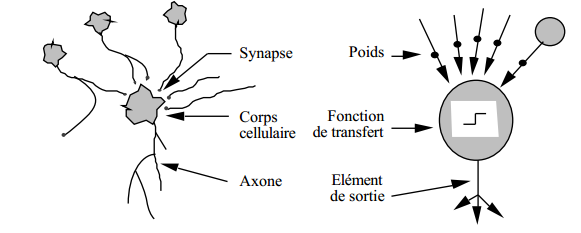
\includegraphics[scale=0.4]{images/chapter1/neurone_bio.png}\label{neurone}}
  \caption{Conception d'un neurone artificiel à partir d'un neurone biologique \\ Source : https://sites.google.com/site/tpeia9/home}
\end{center}
\end{figure}

\section{Un neurone}

\begin{definition}[Neurone]
Un neurone est modélisé par une fonction $f$ de $\mathbb{R}^n$ dans $\mathbb{R}$. Elle est déterminée par trois paramètres : un vecteur de poids $w \in \mathbb{R}^n$, un biais $b \in \mathbb{R}$ et une fonction d'activation $g$. La fonction $f$ se réécrit alors :

\begin{equation}
\forall x \in \mathbb{R}^n, y = f(x) = g(w^Tx+b) = g(\sum_{i=1}^{n}{w_ix_i}+b)
\label{sortie_neurone1}
\end{equation}
\end{definition}

\begin{remark}
Il est usuel de rajouter une composante $x_0$ égale à 1 à chaque entrée afin de pouvoir considérer le biais comme un simple poids. Avec cette convention, la formule \ref{sortie_neurone1} devient :

\begin{equation}
\forall x \in \mathbb{R}^n, y = f(x) = g(w^Tx) = g(\sum_{i=0}^{n}{w_ix_i})
\label{sortie_neurone2}
\end{equation}
\end{remark}

L'analogie avec le neurone biologique est ici claire. La fonction prend plusieurs entrées que l'on peut assimiler aux dendrites, les pondère et renvoie une sortie scalaire qui correspond à l'axone.

La figure \ref{neurone} montre une représentation graphique d'un neurone.

\begin{figure}
\begin{center}
\pagestyle{empty}
\begin{tikzpicture}[scale=0.6][line cap=round,line join=round,>=triangle 45,x=1.0cm,y=1.0cm]
\clip(-7.42,-11.35) rectangle (16.51,6.37);
\draw(0,2) circle (1cm);
\draw(0,-1) circle (1cm);
\draw(0,-4) circle (1cm);
\draw(0,-7) circle (1cm);
\draw(7,-2.5) circle (1cm);
\draw [->] (1,2) -- (6,-2.5);
\draw [->] (1,-1) -- (6,-2.5);
\draw [->] (1,-4) -- (6,-2.5);
\draw [->] (1,-7) -- (6,-2.5);
\draw [->] (8,-2.5) -- (10,-2.5);
\draw (8.5,-1.8) node[anchor=north west] {$ y $};
\draw (-1,2.4) node[anchor=north west] {$ x_0=1 $};
\draw (-0.45,-0.7) node[anchor=north west] {$ x_1 $};
\draw (-0.45,-3.7) node[anchor=north west] {$ x_2 $};
\draw (-0.45,-6.7) node[anchor=north west] {$ x_3 $};
\draw (3.3,0.5) node[anchor=north west] {$ w_0 $};
\draw (2.95,-0.9) node[anchor=north west] {$ w_1 $};
\draw (2.95,-2.3) node[anchor=north west] {$ w_2 $};
\draw (3.3,-3.5) node[anchor=north west] {$ w_3 $};
\draw (5.9,-1.9) node[anchor=north west] {$ g(w^Tx) $};
\end{tikzpicture}
\caption{Représentation graphique d'un neurone. Le biais est ici considéré comme le poids associé à une entrée constante égale à 1.}
\label{neurone}
\end{center}
\end{figure}

Les principales fonctions d'activation sont : 

\begin{itemize}
\item $Id : x \mapsto x$ dite identité;
\item $u : x \mapsto 1_{x \geq 0}$ dite échelon ou fonction de Heavyside ;
\item $\tanh : x \mapsto \tanh(x)$ dite tangente hyperbolique ;
\item $\sigma : x \mapsto \frac{1}{1+\exp(-x)}$ dite sigmoïde de part de sa forme en S;
\item $ReLU : x \mapsto max(0, x)$ dite ReLU (rectified linear unit).
\end{itemize}

La figure \ref{fonctions_activation} montre les graphes de ces différentes fonctions et permet de visualiser les différences entre celles-ci.

\begin{figure}
\begin{center}
\begin{tabular}{cc}
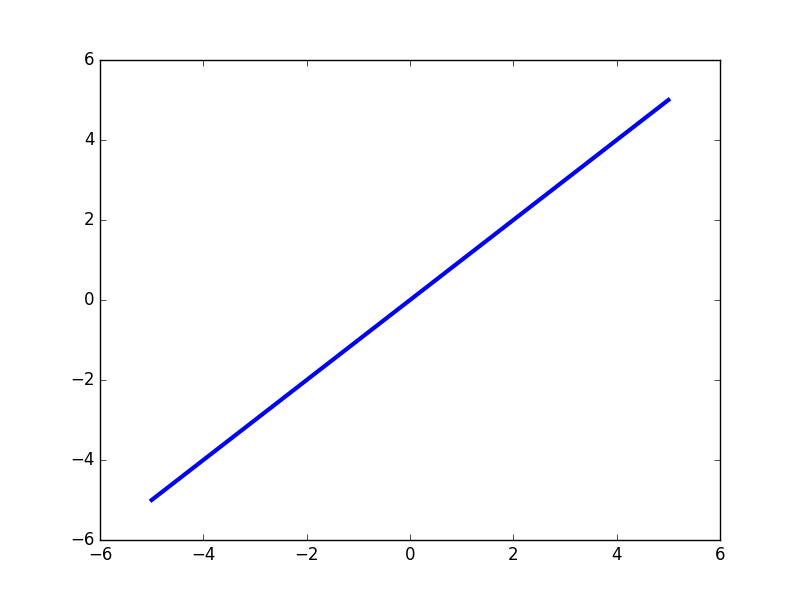
\includegraphics[scale=0.25]{images/chapter1/id.png} & 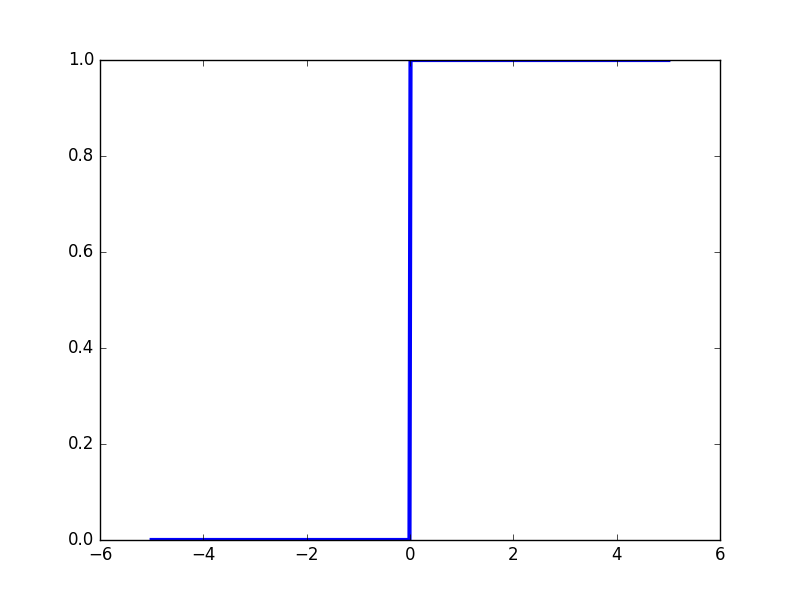
\includegraphics[scale=0.25]{images/chapter1/u.png} \\
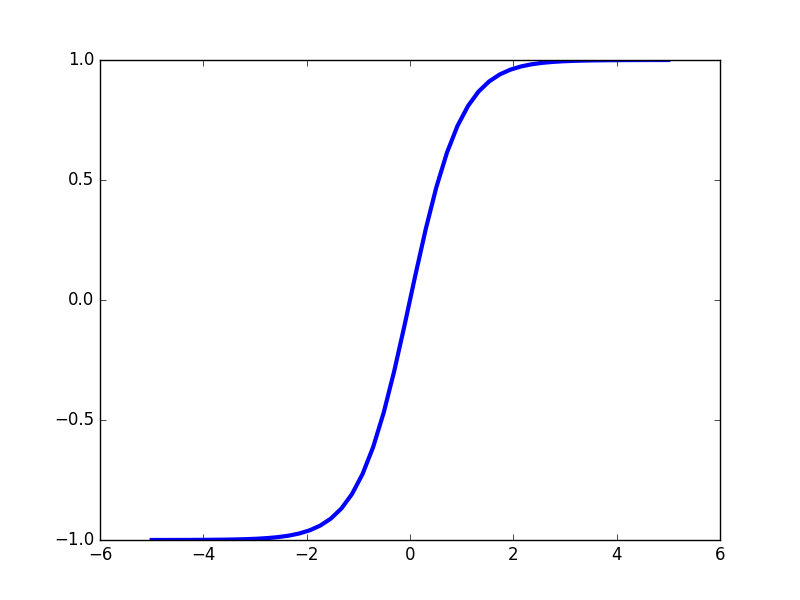
\includegraphics[scale=0.25]{images/chapter1/tanh.png} & 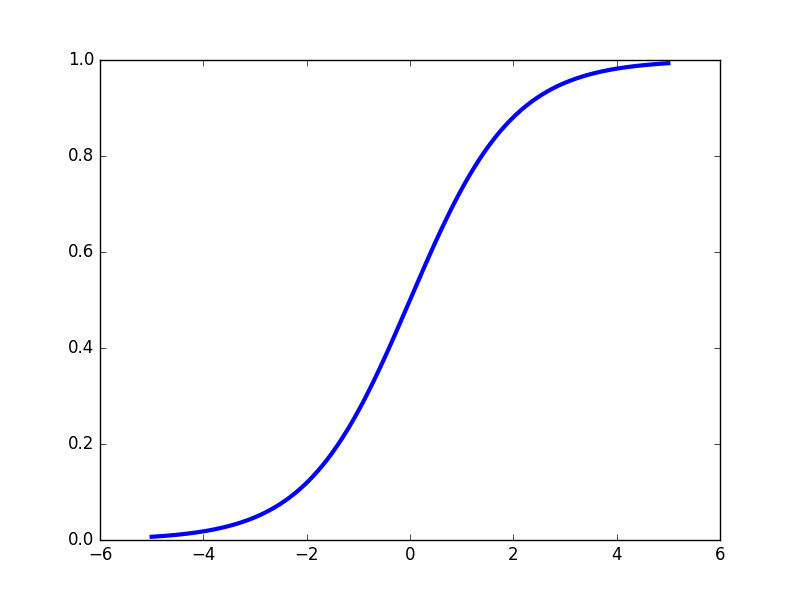
\includegraphics[scale=0.25]{images/chapter1/s.png} \\
\multicolumn{2}{c}{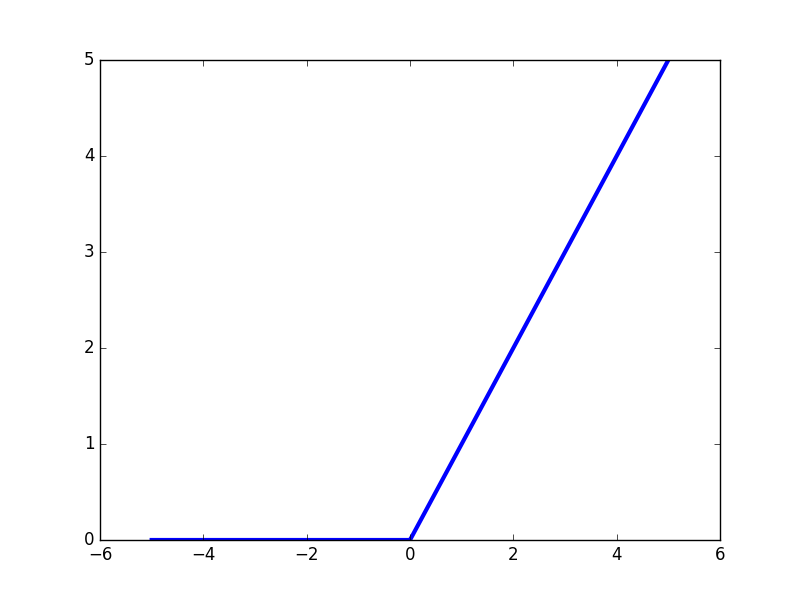
\includegraphics[scale=0.25]{images/chapter1/relu.png}}
\end{tabular}
\caption{Graphe entre -5 et 5 de la fonction identité (en haut à gauche), de l'échelon (en haut à droite), de la tangente hyperbolique (au milieu à gauche), de la sigmoïde (au milieu à droite) et de ReLU (en bas).} 
\label{fonctions_activation}
\end{center}
\end{figure}

Il est possible de se servir d'un neurone seul pour résoudre des problèmes de classification ou de régression. Détaillons quelques exemples importants.

\begin{example}[Perceptron]
Un neurone avec comme fonction d'activation un échelon sépare l'espace en deux demis espaces séparés par un hyperplan de vecteur normal $w$. En effet :

\begin{itemize}
\item $ \forall x \in \mathbb{R}^n, w^Tx < 0 \Rightarrow f(x) = 0$
\item $ \forall x \in \mathbb{R}^n w^Tx \geq 0 \Rightarrow f(x) = 1$
\end{itemize}

La figure \ref{hyperplan} illustre cette séparation. Ce cas particulier de neurone est couramment appelé perceptron.
\end{example}

\begin{figure}
\begin{center}
\pagestyle{empty}
\definecolor{qqqqff}{rgb}{0,0,1}
\definecolor{ffqqqq}{rgb}{1,0,0}
\begin{tikzpicture}[line cap=round,line join=round,>=triangle 45,x=1.0cm,y=1.0cm]
\draw[->,color=black] (-5.42,0) -- (5.45,0);
\foreach \x in {-5,-4,-3,-2,-1,1,2,3,4,5}
\draw[shift={(\x,0)},color=black] (0pt,2pt) -- (0pt,-2pt) node[below] {\footnotesize $\x$};
\draw[->,color=black] (0,-2.99) -- (0,5.07);
\foreach \y in {-2,-1,1,2,3,4,5}
\draw[shift={(0,\y)},color=black] (2pt,0pt) -- (-2pt,0pt) node[left] {\footnotesize $\y$};
\draw[color=black] (0pt,-10pt) node[right] {\footnotesize $0$};
\clip(-5.42,-2.99) rectangle (5.45,5.07);
\fill[line width=0pt,color=ffqqqq,fill=ffqqqq,fill opacity=0.1] (-12.7,-3.03) -- (15.5,5.76) -- (10.12,27.67) -- (-20,20) -- cycle;
\fill[line width=0pt,color=qqqqff,fill=qqqqff,fill opacity=0.1] (-12.7,-3.03) -- (-3.47,-28.78) -- (29.71,-17.95) -- (15.5,5.76) -- cycle;
\draw [domain=-5.42:5.45] plot(\x,{(-1.14-0.38*\x)/-1.22});
\draw [->] (1.12,1.28) -- (0.74,2.5);
\draw (0.74,2.89) node[anchor=north west] {$ w $};
\end{tikzpicture}
\caption{Hyperplan séparateur dans un espace à deux dimensions correspondant à un certain vecteur de poids $w$. La partie rouge correspond aux entrées classifiées 1 et en bleue celles qui sont classifiées 0.}
\label{hyperplan}
\end{center}
\end{figure}

\begin{example}[Régression logistique]
Si la fonction d'activation est une sigmoïde, la sortie du neurone peut être interprétée comme la probabilité $p(y=1|x)$. Par conséquent, le neurone classifie un exemple dans la classe 1 si la sortie est supérieure à $0.5$ et dans la classe 0 sinon. On parle ici de régression logistique. L'espace est toujours séparée en deux parties par un hyperplan, $H = \{x, f(x)=0.5\}$. Cependant maintenant les valeurs associées aux entrées sont continues entre $0$ et $1$. La figure \ref{regression_logistique} permet de visualiser cette différence. Dans la suite de ce document, des graphes de ce type seront utilisés à plusieurs reprises afin de pouvoir visualiser l'action d'un réseau de neurones.
\end{example}

\begin{figure}
\begin{center}
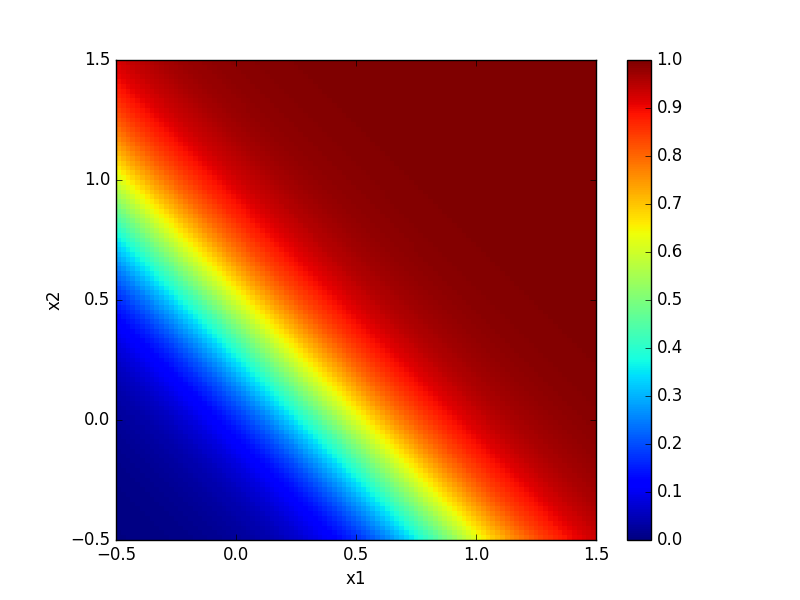
\includegraphics[scale=0.5]{images/chapter1/or.png}
\caption{Sortie d'une régression logistique prenant en entrée un vecteur de $\mathbb{R}^2$ sur $[-0.5, 1.5] \times [-0.5, 1.5]$. L'axe $x_1$ et l'axe $x_2$ correspondent respectivement à la première et à la deuxième coordonnée de l'entrée.}
\label{regression_logistique}
\end{center}
\end{figure}

\begin{example}[Régression linéaire]
Finalement, si la fonction d'activation est la fonction identité, le neurone sera capable d'atteindre toutes les valeurs réelles. Il pourra donc résoudre un problème de régression. Il s'agit de la régression linéaire.
\end{example}

Le point commun entre tous les neurones est qu'ils sont seulement capable de modéliser des interactions linéaires entre les entrées. Cependant, à partir d'un ensemble de données, il est possible d'utiliser des neurones pour modéliser des interactions non linéaires entre les différentes composantes des entrées. Pour cela, il faut transformer les entrées afin de créer de nouvelles composantes. Par exemple, prenons un ensemble de données tel que les points ont le label $1$ s'ils sont dans le disque de rayon 0.5 et de centre $(0;0)$ et $0$ sinon. Un exemple d'un tel ensemble de donnée est visible sur la figure \ref{disque}. En l'état, cet ensemble n'est pas linéairement séparable et donc un neurone simple ne peut pas le classifier correctement. Cependant si une transformation telle que $x \mapsto (x_1, x_2, x_1x_2, x_1^2, x_2^2)$ est appliquée aux exemples. Les points sont maintenant linéairement séparables dans ce nouvel espace. Il est alors possible d'utiliser un neurone afin de classifier correctement l'ensemble. Ces résultats sont présents sur la figure \ref{disque}.

\begin{figure}
\begin{center}
\begin{tabular}{cc}
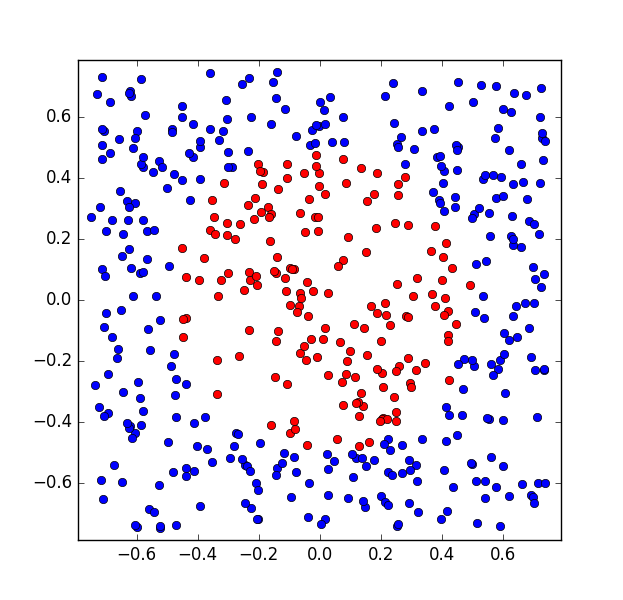
\includegraphics[scale=0.35]{images/chapter1/disk_dataset.png} & 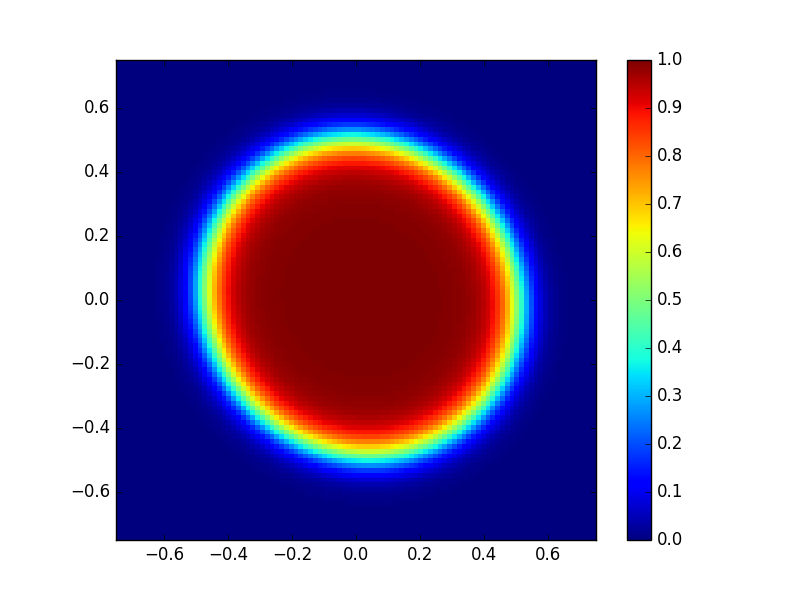
\includegraphics[scale=0.35]{images/chapter1/disk_learned.png} \\
\end{tabular}
\caption{À gauche un ensemble de données de 500 points. Les points à l'intérieur du cercle de rayon 0.5 et de centre $(0; 0)$ sont en rouge, les autres en bleu. À droite, la représentation du disque apprise par le neurone.} 
\label{disque}
\end{center}
\end{figure}

En conclusion, un neurone est une fonction relativement simple permettant de modéliser des interactions linéaires entre ses entrées. Dans la partie suivante, nous verrons comment associer ces neurones afin de créer des modèles plus complexes.

\section{Un réseau de neurones}

\begin{definition}[Réseau de neurones]
Un réseau de neurones est défini par un graphe orienté $\mathcal{G}(V, A)$ où les n\oe{}uds sont des neurones et les arêtes des liens entre les neurones et par un ensemble de neurones d'entrée $V_{in} \subset V$ et de neurones de sorties $V_{out} \subset V$. Une arête partant d'un neurone $i$ vers un neurone $j$ signifie que la sortie du neurone $i$ est une entrée pour le neurone $j$. Notons $f_{j}$ la fonction représentant le neurone $j$. Finalement, nous noterons un réseau $\mathcal{N}(V, A, V_{in}, V_{out}, f)$ où $f$ est l'ensemble des fonctions des neurones.
\end{definition}

Si nous notons $Pa$ l'application qui à un neurone renvoie les indices de ses parents et $Ch$ l'application qui à un neurone renvoie les indices de ses enfants. Alors la sortie du neurone $j$ est :

\begin{equation}
y_{j} = f_{j}((y_{i})_{i \in Pa(j)})
\label{eq_propagation}
\end{equation} 

Il existe certaines classes particulière de réseau de neurones. Tout d'abord, s'il contient des cycles, il sera dit récurrent. Dans le cas contraire, on parlera de réseau \textit{feedforward}. Puis s'il est possible de l'organiser sous forme de couches où les sorties des neurones d'une couche sont les entrées de la couche suivante, on parle de réseau de neurones multicouche dit aussi MLP (multilayer perceptron). Des exemples des différents types de réseaux sont présents sur la figure \ref{reseaux}.

\begin{figure}
\begin{center}
\begin{tabular}{cc}
\begin{tikzpicture}[scale=0.30][line cap=round,line join=round,>=triangle 45,x=1.0cm,y=1.0cm]
\clip(-3.5,-5.5) rectangle (13.5,7);
\draw(-1,4) circle (1cm);
\draw(-1,1) circle (1cm);
\draw(-1,-2) circle (1cm);
\draw(3,3) circle (1cm);
\draw(3,-1) circle (1cm);
\draw(7,3) circle (1cm);
\draw(11,3) circle (1cm);
\draw(11,-1) circle (1cm);
\draw [->] (0,4) -- (2,3);
\draw [->] (0,1) -- (2,3);
\draw [->] (0,-2) -- (2,-1);
\draw [->] (0,1) -- (2,-1);
\draw [->] (3,0) -- (3,2);
\draw(7,-1) circle (1cm);
\draw [->] (7,2) -- (4,-1);
\draw [->] (4,3) -- (6,3);
\draw [->] (4,-1) -- (6,-1);
\draw [->] (7,0) -- (7,2);
\draw [->] (8,3) -- (10,3);
\draw [->] (8,-1) -- (10,-1);
\draw [rotate around={90:(-1,1)},dash pattern=on 3pt off 3pt] (-1,1) ellipse (5.22cm and 1.5cm);
\draw (-3.5,-4.15) node[anchor=north west] {$ Entrées $};
\draw [rotate around={90:(11,1)},dash pattern=on 3pt off 3pt] (11,1) ellipse (4.25cm and 1.45cm);
\draw (8.8,-3.21) node[anchor=north west] {$ Sorties $};
\draw (-1.7,4.6) node[anchor=north west] {$ 1 $};
\draw (-1.95,1.6) node[anchor=north west] {$ x_1 $};
\draw (-1.95,-1.4) node[anchor=north west] {$ x_2 $};
\draw (2.1,3.9) node[anchor=north west] {$ f_1 $};
\draw (2.1,-0.1) node[anchor=north west] {$ f_2 $};
\draw (6,3.9) node[anchor=north west] {$ f_3 $};
\draw (6,-0.1) node[anchor=north west] {$ f_4 $};
\draw (10,3.7) node[anchor=north west] {$ y_1 $};
\draw (10,-0.3) node[anchor=north west] {$ y_2 $};
\end{tikzpicture} & \begin{tikzpicture}[scale=0.3][line cap=round,line join=round,>=triangle 45,x=1.0cm,y=1.0cm]
\clip(-3.94,-7.74) rectangle (13.14,4.91);
\draw(-1,2) circle (1cm);
\draw(-1,-1) circle (1cm);
\draw(-1,-4) circle (1cm);
\draw(3,1) circle (1cm);
\draw(3,-3) circle (1cm);
\draw(7,-1) circle (1cm);
\draw(11,-1) circle (1cm);
\draw [->] (0,2) -- (2,1);
\draw [->] (0,-1) -- (2,1);
\draw [->] (0,-4) -- (2,-3);
\draw [->] (4,1) -- (6,-1);
\draw [->] (3,-2) -- (3,0);
\draw [->] (6,-1) -- (4,-3);
\draw [->] (8,-1) -- (10,-1);
\draw [rotate around={0:(4.5,-1)},dash pattern=on 3pt off 3pt] (4.5,-1) ellipse (3.81cm and 3.5cm);
\draw (2.7,-4.43) node[anchor=north west] {$ Cycle $};
\end{tikzpicture} \\
\begin{tikzpicture}[scale=0.3][line cap=round,line join=round,>=triangle 45,x=1.0cm,y=1.0cm]
\clip(-3.8,-5.74) rectangle (12.92,6.64);
\draw(-1,1) circle (1cm);
\draw(-1,4) circle (1cm);
\draw(-1,-2) circle (1cm);
\draw(3,4) circle (1cm);
\draw(3,-2) circle (1cm);
\draw(3,1) circle (1cm);
\draw(7,1) circle (1cm);
\draw(10,4) circle (1cm);
\draw(10,-2) circle (1cm);
\draw [->] (0,4) -- (2,4);
\draw [->] (0,1) -- (2,4);
\draw [->] (0,1) -- (2,-2);
\draw [->] (0,-2) -- (2,-2);
\draw [->] (3,-1) -- (3,0);
\draw [->] (3,3) -- (3,2);
\draw [->] (4,1) -- (6,1);
\draw [->] (4,-2) -- (6,1);
\draw [->] (4,4) -- (6,1);
\draw [->] (8,1) -- (9,4);
\draw [->] (8,1) -- (9,-2);
\draw [->] (4,-2) -- (9,-2);
\draw [->] (4,4) -- (9,4);
\end{tikzpicture} & \begin{tikzpicture}[scale=0.24][line cap=round,line join=round,>=triangle 45,x=1.0cm,y=1.0cm]
\clip(-8.76,-5.24) rectangle (13.65,11.36);
\draw(-2,6) circle (1cm);
\draw(-2,3) circle (1cm);
\draw(-2,0) circle (1cm);
\draw(2,3) circle (1cm);
\draw(2,6) circle (1cm);
\draw(2,0) circle (1cm);
\draw(2,-3) circle (1cm);
\draw(2,9) circle (1cm);
\draw(6,6) circle (1cm);
\draw(6,3) circle (1cm);
\draw(6,0) circle (1cm);
\draw(10,3) circle (1cm);
\draw [->] (-1,6) -- (1,9);
\draw [->] (-1,6) -- (1,6);
\draw [->] (-1,6) -- (1,3);
\draw [->] (-1,6) -- (1,0);
\draw [->] (-1,3) -- (1,9);
\draw [->] (-1,3) -- (1,6);
\draw [->] (-1,3) -- (1,3);
\draw [->] (-1,3) -- (1,0);
\draw [->] (-1,0) -- (1,0);
\draw [->] (-1,0) -- (1,3);
\draw [->] (-1,0) -- (1,6);
\draw [->] (-1,0) -- (1,9);
\draw [->] (3,9) -- (5,6);
\draw [->] (3,6) -- (5,6);
\draw [->] (3,3) -- (5,6);
\draw [->] (3,0) -- (5,6);
\draw [->] (3,6) -- (5,3);
\draw [->] (3,3) -- (5,3);
\draw [->] (3,3) -- (5,0);
\draw [->] (3,9) -- (5,3);
\draw [->] (3,9) -- (5,0);
\draw [->] (3,6) -- (5,0);
\draw [->] (3,0) -- (5,0);
\draw [->] (3,0) -- (5,3);
\draw [->] (-1,6) -- (1,-3);
\draw [->] (-1,3) -- (1,-3);
\draw [->] (-1,0) -- (1,-3);
\draw [->] (3,-3) -- (5,0);
\draw [->] (3,-3) -- (5,3);
\draw [->] (3,-3) -- (5,6);
\draw [->] (7,6) -- (9,3);
\draw [->] (7,3) -- (9,3);
\draw [->] (7,0) -- (9,3);
\end{tikzpicture} \\
\end{tabular}
\caption{Exemples de réseaux de neurones. Un réseau de neurones quelconque (en haut à gauche),  récurrent (en haut à droite), feedforward (en bas à gauche) et multicouche (en bas à droite).} 
\label{reseaux}
\end{center}
\end{figure}

Dans les sections suivantes, seront étudiés les algorithmes pour évaluer un réseau de neurones puis pour l’entraîner. Cependant, seulement les algorithmes dans le cadre d'un réseau de neurones feedforward seront abordés. Les algorithmes concernant les réseaux de neurones récurrent seront abordés dans la partie \autoref{chap:Réseaux de neurones récurrents}.

\section{Propagation}

L'algorithme de propagation dans le cadre des réseaux feedforward est très simple. Il suffit de mettre à jour les neurones d'entrée puis d'appliquer la formule \ref{eq_propagation} récursivement en partant des neurones dans $V_{out}$.

Ainsi, un premier algorithme naïf est :

\begin{algorithm} 
\begin{algorithmic}
\Procedure{$evaluer\_reseau$}{$\mathcal{N}(V, A, V_{in}, V_{out}, f), x$}
\Function{$evaluer\_neurone$}{$j$}
	\If{$j \in V_{in}$}
    	\State \Return $x_j$
	\Else
		\State $t \leftarrow (evaluer\_neurone(i), i \in Pa(j))$
		\State \Return $f_j(t)$
	\EndIf
\EndFunction

\For{$j \in V_{out}$}
	\State $y_j \leftarrow evaluer\_neurone(j)$ 
\EndFor
\EndProcedure
\end{algorithmic} 
\caption{Algorithme naïf d'évaluation d'un réseau de neurone feedforward. Il prend en entrée un réseau de neurone et un vecteur d'entrée pour le réseau de neurone.}
\end{algorithm}

Cette version n'est pas du tout efficace, elle calcule plusieurs fois la sortie de chaque neurone. Si le graphe est densément connecté, l'algorithme aura un coût temporel extrêmement élevé. Une amélioration simple consiste à rajouter de la mémoïsation afin de garantir que la sortie de chaque neurone sera calculée au plus une fois. Le pseudo-code de cet algorithme correspond à l'algorithme \ref{propagation_memoisation}.

\begin{algorithm} 
\begin{algorithmic}
\Procedure{$evaluer\_reseau$}{$\mathcal{N}(V, A, V_{in}, V_{out}, f), x$}
\Function{$evaluer\_neurone$}{$j$}
	\If{$déjàCalculé[j]$ est $faux$}
		\State $t \leftarrow (evaluer\_neurone(i), i \in Pa(j))$
		\State $y_j \leftarrow f_j(t)$
		\State $déjàCalculé[j] \leftarrow vrai$
	\EndIf
	\State \Return $y_j$
\EndFunction

\State Initialiser un tableau $dejaCalculé$ de longueur $|V|$ à $faux$.
\For{$i \in V_{in}$}
	\State $y_i \leftarrow x_i$
	\State $déjàCalculé[i] \leftarrow vrai$ 
\EndFor
\For{$j \in V_{out}$}
	\State $evaluer\_neurone(j)$ 
\EndFor
\EndProcedure
\end{algorithmic}
\caption{Algorithme d'évaluation d'un réseau de neurone feedforward utilisant la mémoïsation afin de ne pas recalculer plusieurs fois la sortie d'un neurone.}
\label{propagation_memoisation}
\end{algorithm}

Cet algorithme calcule au plus une fois la sortie de chaque neurone et il appelle $evaluer\_neurone$ au plus $|A|$ fois, il a donc un coût temporel en $O(|V|+|A|)$. Ce qui est a priori le coût optimal.

\section{Fonctions de coût}

Avant de parler des algorithmes d'apprentissage et de la manière de modifier les poids avant d'approcher une fonction, nous allons revenir sur les fonctions de coût. Dans la suite, nous justifierons l'utilisation et le bien-fondé des fonctions de coût les plus courantes.

Il sera détaillé trois fonctions de coût : une pour la régression, une pour la classification binaire et une pour la classification à plusieurs classes. La même méthode sera utilisée à chaque fois : un modèle sera proposé puis la fonction de coût sera déduite en utilisant le principe du maximum de vraisemblance.

\begin{definition}[Fonction de vraisemblance]
Si $x_1, ..., x_n$ sont des échantillons générés indépendamment par une probabilité $p_{\theta}$ la vraisemblance de l'échantillon est alors :
$$
L(\theta) = \prod_{i=1}^{N}{p_{\theta}(x^{(i)})}
$$
\end{definition}

\begin{remark}
Dans notre cas, les échantillons $(x_1, y_1), ..., (x_n, y_n)$ sont générés par la loi $p_{\theta}(y|x)$ où $\theta$ sont les paramètres du modèle, la vraisemblance est donc :
$$
L(\theta) = \prod_{i=1}^{N}{p_{\theta}(y^{(i)}|x^{(i)})}
$$
\end{remark}

\begin{definition}[Maximum de vraisemblance]
Le paramètre $\theta$ maximise la vraisemblance si $\theta \in argmax L(\theta')$.
\end{definition}

\begin{remark}
Maximiser la vraisemblance revient donc à rechercher le maximum d'une fonction.
\end{remark}

\begin{remark}
Au lieu de maximiser la vraisemblance, nous allons minimiser l'opposé du logarithme de la vraisemblance (\textit{negative log-likelihood} en anglais). On obtient alors :
\begin{equation}
NLL(\theta) = -\sum_{i=1}^{N}{\log{p_{\theta}(y^{(i)}|x^{(i)})}}
\label{NLL}
\end{equation}
Cette forme est préférée car la somme est plus facile à dériver que le produit. En outre, l'opposé du logarithme de la vraisemblance est pris pour se ramener à un problème de minimisation.
\end{remark}

\subsection{Régression}

Dans un problème de régression, il est courant de choisir comme modèle :

\begin{equation}
p_{\theta}(y|x) \sim \mathcal{N}(\hat{y}(x, \theta), \sigma) \Leftrightarrow p_{\theta}(y|x) = \frac{1}{\sqrt{2\pi}\sigma}\exp{(\frac{-(y - \hat{y})^2}{2\sigma^2})}
\label{modele_normale}
\end{equation}

Où $\theta$ est l'ensemble des poids de notre réseau, $\hat{y}(x, \theta)$ est la sortie de notre réseau quand l'entrée est $x$ et $\sigma$ une constante positive. On se permettra de noter seulement $\hat{y}(x)$ au lieu de $\hat{y}(x, \theta)$ pour plus de légèreté.


En remplaçant $p_{\theta}$ par l'expression \ref{modele_normale} dans l'équation \ref{NLL}, on obtient :

\begin{equation}
NLL(\theta) = \sum_{i=1}^{N}{(y^{(i)} - \hat{y}(x^{(i)}))^2} + C
\end{equation}

où $C$ est une constante.

Dans le problème de minimisation, la constante peut être négligée et il est possible de multiplier par une constante positive sans changer le problème. On déduit que sous cette modélisation, une fonction de coût obtenue par le principe de maximum de vraisemblance est :

\begin{equation}
E = \frac{1}{N}\sum_{i=1}^{N}{(y^{(i)} - \hat{y}(x^{(i)}))^2} = \frac{1}{N}\sum_{i=1}^{N}{e(y^{(i)}, \hat{y}(x^{(i)}))}
\end{equation}

avec $e : (x, y) \mapsto (x - y)^2$. Cette fonction est appelée erreur quadratique moyenne (\textit{mean squared error} en anglais).

\subsection{Classification binaire}

Dans le cas de la classification binaire, à $x$ fixé, $p(y|x)$ suit une loi de Bernoulli. Un modèle possible est donc :

\begin{equation}
p_{\theta}(y|x) \sim \mathcal{B}(\hat{y}(x, \theta)) \Leftrightarrow p_{\theta}(y|x) = 
\left\{
    \begin{array}{ll}
        \hat{y}(x) \text{ si } y = 1 \\
        1 - \hat{y}(x) \text{ sinon}
    \end{array}
\right.
\label{modele_bernoulli}
\end{equation}

La formule \ref{modele_bernoulli} peut se réécrire de manière plus compacte :
\begin{equation}
p_{\theta}(y|x) = \hat{y}(x)^y(1-\hat{y}(x))^{1-y}
\label{modele_bernoulli_compact}
\end{equation}

En utilisant cette dernière forme, on obtient que l'expression de la \textit{negative log-likelihood} est : 

\begin{equation}
NLL(\theta) = -\sum_{i=1}^{N}{y^{(i)}\log\hat{y}(x^{(i)})+(1-y^{(i)})\log(1-\hat{y}(x^{(i)}))}
\end{equation}

On en déduit de même que précédemment que notre fonction de coût est :

\begin{equation}
E = \frac{1}{N}\sum_{i=1}^{N}{-(y^{(i)}\log\hat{y}(x^{(i)})+(1-y^{(i)})\log(1-\hat{y}(x^{(i)})))} = \frac{1}{N}\sum_{i=1}^{N}{e(y^{(i)}, \hat{y}(x^{(i)}))}
\end{equation}

avec $e : (x, y) \mapsto -(x \log y + (1-x)\log(1-y))$.

\subsection{Classification à plusieurs classes}

Finalement, dans le cas d'une classification à plusieurs classes, $p(y|x)$ est une loi Multinoulli à $x$ fixé. Si la sortie $\hat{y}$ du réseau est un vecteur de longueur $M$ avec $M$ le nombre de classes, une sortie possible est :

\begin{equation}
p_{\theta}(y|x) \sim \mathcal{M}(\hat{y}(x, \theta)_0, ..., \hat{y}(x, \theta)_{M-1}) \Leftrightarrow p_{\theta}(y|x) = \hat{y}(x)_y
\label{modele_multinoulli}
\end{equation}

La \textit{negative log-likelihood} associée est donc :

\begin{equation}
NLL(\theta) = -\sum_{i=1}^{N}{\log \hat{y}(x^{(i)})_{y^{(i)}}}
\label{NLL_multinoulli}
\end{equation}

Posons pour tout $i \in \{0, ..., M-1\}$, $\tau^{(i)} \in \mathbb{R}^M$ le vecteur tel que :

$$ \tau^{(i)}_j = 
\left\{
    \begin{array}{ll}
        1 \text{ si } i = j \\
        0 \text{ sinon}
    \end{array}
\right.
$$

Il est alors possible de réécrire la formule \ref{NLL_multinoulli} en utilisant ces vecteurs :

\begin{equation}
NLL(\theta) = \sum_{i=1}^{N}{-\sum_{j=0}^{M-1}{\tau^{(y^{(i)})}_j\log \hat{y}(x^{(i)})_j}}
\end{equation}

Enfin en introduisant l'entropie croisée $H$ définie de manière générale par :

$$
H(p, q) = -\sum_{x}{p(x)\log q(x)}
$$

On obtient que :

\begin{equation}
NLL(\theta) = \sum_{i=1}^{N}{H(\tau^{(y^{(i)})}, \hat{y}(x^{(i)}))}
\end{equation}

On a remplacé $y$ par un vecteur prenant un $1$ à la position $y$, une telle transformation est couramment appelé encodage \textit{one-hot}. 

Notre fonction de coût sera donc :

\begin{equation}
E = \frac{1}{N}\sum_{i=1}^{N}{H(\tau^{(y^{(i)})}, \hat{y}(x^{(i)}))} = \frac{1}{N}\sum_{i=1}^{N}{e(y^{(i)}, \hat{y}(x^{(i)}))}
\end{equation}

Avec $e : (x, y) \mapsto H(\tau^x, y)$. Cette fonction de coût est naturellement appelée entropie croisée (\textit{cross-entropy} en anglais).

\section{Descente du gradient}

Étant donné une fonction de coût $E$, l'objectif de l'apprentissage est de déterminer les poids permettant de minimiser $E$. Dans l'idéal, il faudrait pouvoir exprimer $E$ en fonction des poids, dériver $E$ par rapport à chaque poids puis chercher les valeurs des poids atteignant les minimas. Malheureusement, dans la plupart des cas, il est impossible d'avoir de telles solutions analytiques.

Une réponse à ce problème est la descente du gradient. Le principe est simple, il s'agit d'un procédé itératif consistant à modifier légèrement les valeurs des poids afin qu'à chaque étape $E$ décroisse.  En notant, $\theta$ le vecteur contenant les poids de tous les neurones du réseau. La valeur de ces poids changera à chaque itération, par conséquent, notons $\theta(t)$ la valeur de $\theta$ à l'itération $t$. La direction selon laquelle $E$ augmente le plus est $\frac{\partial E}{\partial \theta}$, la direction selon laquelle $E$ décroît le plus est donc $-\frac{\partial E}{\partial \theta}$. Si les poids sont modifiés en se déplaçant dans cette direction d'un pas $\eta(t)$ assez petit, le coût diminuera. L'équation d'évolution est donnée par \ref{mise_a_jour_poids}.

\begin{equation}
\theta(t+1) = \theta(t) - \eta(t) \frac{\partial E}{\partial \theta}
\label{mise_a_jour_poids}
\end{equation}

Il existe plusieurs stratégies afin de choisir le pas $\eta(t)$. Dans un premier temps et pour plus de simplicité, nous choisirons un pas $\eta(t)=\eta$ constant.

\section{Rétropropagation du gradient}

L'application de l'algorithme précédant nécessite le calcul des dérivées partielles par rapport à chacun des poids du réseau de neurones. Prenons le neurone $j$ du réseau de neurone. Son entrée est notée $x_j$, sa sortie $y_j$, sa fonction d'activation $g_j$ et ses poids $w_j$. De plus, définissons la quantité intermédiaire $s_j = w_j^Tx_j$. La formule \ref{sortie_neurone2} appliquée à ce neurone est donc $y_j = g_j(w_j^Tx_j) = g(s_j)$. En utilisant la règle de la chaîne, on obtient que :

\begin{equation}
\frac{\partial E}{\partial w_j} = \frac{\partial E}{\partial y_j}\frac{\partial y_j}{\partial s_j}\frac{\partial s_j}{\partial w_j}
\label{dEdw_avant}
\end{equation}

On peut remarquer que le terme $\frac{\partial s_j}{\partial w_j}$ est égal à $x_j$ et que $\frac{\partial y_j}{\partial s_j} = g'(s_j)$ d'où l'égalité \ref{dEdw_avant} devient :

\begin{equation}
\frac{\partial E}{\partial w_j} = \frac{\partial E}{\partial y_j} g_j'(s_j) x_j
\label{dEdw}
\end{equation}

Afin de calculer $\frac{\partial E}{\partial y_j}$, utilisons le fait que la sortie du neurone $j$ est une des entrées de ses enfants. En notant $x_{i, j}$ l'entrée du neurone i correspondant à la sortie du neurone $j$, on a :

\begin{equation}
\frac{\partial E}{\partial y_j} = \sum_{i \in Ch(j)}{\frac{\partial E}{\partial x_{i,j}}}
\label{formule_retropropagation}
\end{equation}

La formule \ref{formule_retropropagation} montre que si on calcule $\frac{\partial E}{\partial x_i}$, la dérivée du coût par rapport aux entrées d'un neurone, il est aisé de calculer la dérivée du coût par rapport aux poids pour les parents de ce neurone. Or la dérivée du coût par rapport aux entrées d'un neurone est facilement calculable en utilisant l'égalité suivante :

\begin{equation}
\frac{\partial E}{\partial x_j} = \frac{\partial E}{\partial y_j}\frac{\partial y_j}{\partial s_j}\frac{\partial s_j}{\partial x_j} =  \frac{\partial E}{\partial y_j} g_j'(s_j) w_j
\label{dEdx}
\end{equation}

Finalement, en utilisant les formules \ref{dEdw}, \ref{formule_retropropagation} et \ref{dEdx}, il est possible de rétropropager le gradient et de calculer $\frac{\partial E}{\partial w_j}$ pour tout neurone $j$. On en déduit l'algorithme suivant :

\begin{algorithm} 
\begin{algorithmic}
\Procedure{$retropropager\_gradient$}{$\mathcal{N}(V, A, V_{in}, V_{out}, f), x, y$}
\Function{$calculer\_gradient$}{$j$}
	\If{$déjàCalculé_j$ est $faux$}
		\State $\frac{\partial E}{\partial y_j} \leftarrow \sum_{i \in Ch(j)}{calculer\_gradient(i)_j}$
		\State $\frac{\partial E}{\partial x_j} \leftarrow \frac{\partial E}{\partial y_j} g_j'(s_j) w_j$
		\State $\frac{\partial E}{\partial w_j} \leftarrow \frac{\partial E}{\partial y_j} g_j'(s_j) x_j$
		\State $déjàCalculé_j \leftarrow vrai$
	\EndIf
	\State \Return $\frac{\partial E}{\partial x_j}$
\EndFunction

\State Appeler $evaluer\_reseau(\mathcal{N}(V, A, V_{in}, V_{out}, f), x)$ et récupérer les entrées et sorties de chaque neurone
\State Initialiser un tableau $dejaCalculé$ de longueur $|V|$ à $faux$.
\For{$i \in V_{out}$}
	\State Calculer $\frac{\partial E}{\partial y_i}$
	\State $déjàCalculé_i \leftarrow vrai$ 
\EndFor
\For{$i \in V$}
	\State $calculer\_gradient(i)$ 
\EndFor
\EndProcedure
\end{algorithmic} 
\caption{Algorithme de rétropropagation du gradient dans un réseau de neurone feedforward.}
\label{propagation_memoisation2}
\end{algorithm}

Cet algorithme utilise la mémoïsation afin de ne pas calculer plusieurs fois les dérivées pour un neurone. On peut remarquer que cet algorithme est très similaire à celui de la propagation. Pour des raisons similaires, le coût temporel de la rétropropagation est aussi en $O(|V|+|A|)$.

\chapter{Une première implémentation}

\section{Motivation}

La première implantation a été faite sous Python avec pour but principal de rester le plus proche possible de l'architecture neuronale du réseau afin de pouvoir bien étudier le fonctionnement de l'algorithme d'apprentissage. Quitte à perdre en rapidité de calcul, nous avons ainsi décidé de créer des éléments neurones et un réseau composé de plusieurs de ces neurones. Cette approche permet une bonne compréhension des concepts de base des réseaux de neurones. Nous avons alors pu appliquer cette implémentation sur des cas simples (XOR notamment, cf Résultats), mais aussi obtenir un aperçu des optimisations possibles afin d'accélérer les calculs. Cela s'est effectivement rapidement révélé nécessaire.  

\section{Diagramme UML}

Suivant cette volonté de créer une première implémentation simple et intuitive, le diagramme UML comporte ainsi deux classes principales : une classe Neuron et une classe Network. Ainsi un réseau (network) sera composé de plusieurs neurones (neurons).

Le neurone a été défini comme une entité autonome, qui comporte des entrées et une sortie et est caractérisé par des poids ainsi que ses relations avec d'autres neurones (parents ou enfants). Il peut alors calculer la sortie si les sorties de ses parents ont préalablement été évaluées. Pour déterminer le gradient au niveau de chaque poids, il a tout d'abord besoin de ceux de ses enfants.


\begin{figure}
\begin{center}
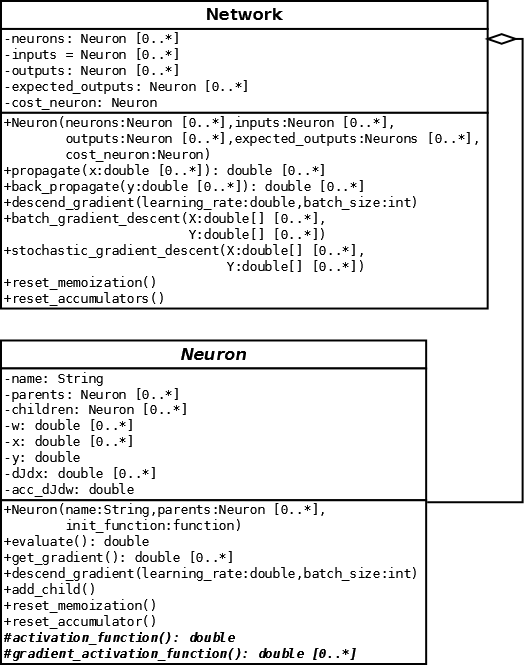
\includegraphics[scale=0.3]{images/uml_simplifie_maispastrop_imp1.png}
\caption{Diagramme UML des clsses Neuron et Network}
\label{Diagramme UML des classes Neuron et Network}
\end{center}
\end{figure}

On répartit les neurones en différentes catégories selon leurs fonctions d'activation (sigmoïde, tangente hyperbolique, Softmax ou ReLu par exemple).

Ainsi la classe Neuron possède de nombreuses sous-classes correspondant à ces fonctions. En outre, il existe plusieurs sous-classes destinées aux neurones ayant un comportement particulier. On distingue ainsi BiasNeuron, qui permet d'ajouter un biais au niveau des entrées d'un autre neurone, InputNeuron correspondant simplement aux neurones d'entrées. L'ajout d'un neurone de coût (cost neuron) à la fin du réseau permet de calculer directement l'erreur lors de la propagation d'une entrée. Il faudra ainsi spécifier pour chaque input d'entrée la sortie attendue pour calculer le coût (avec un InputNeuron).

\begin{figure}
\begin{center}
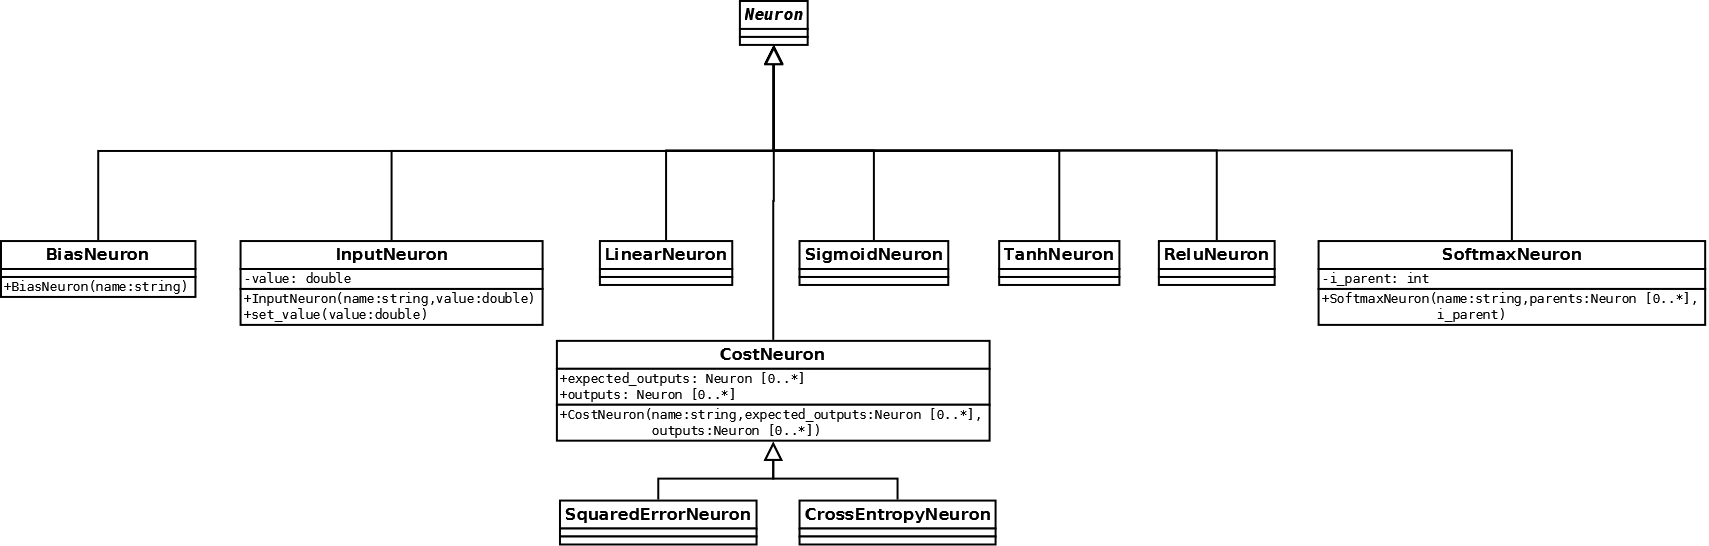
\includegraphics[scale=0.18]{images/uml_neurone_imp1.png}
\caption{Décomposition de la classe neurone}
\label{uml_neurone_imp1}
\end{center}
\end{figure}


Les liens entre neurones ne seront pas mémorisées par le réseau. Cette tâche sera réalisée par les neurones eux-mêmes. Ainsi, chacun possédera en attribut une liste de parents et une liste d'enfants, ce qui lui permettra de se situer dans le réseau. Ces deux listes sont indispensables afin de propager le résultat de sortie du neurone et afin de rétropropager le gradient lors de l'algorithme d'apprentissage.
	
\section{Principe de fonctionnement}
Pour utiliser le programme, il suffit de créer le réseau de neurones voulu. On crée pour cela différents neurones (InputNeuron, SigmoidNeuron, CrossEntropyNeuron, ...) en spécifiant les parents à chaque fois. Le programme mettra lui même à jour les listes de parents et d'enfants de chaque neurone afin de créer les différentes relations entre neurones. On crée finalement le réseau (Network) en spécifiant les entrées, sorties, le neurone de coût et les neurones intermédiaires.
On peut alors appliquer deux fonctions principales sur le réseau. "Propagate" permet de calculer la sortie du réseau pour une entrée fournie en paramètre. "Batch\_propagation\_descent" permet d'appliquer l'algorithme de d'apprentissage basée sur la backpropagation du gradient pour un ensemble d'entrées, de sorties attendues et un learning rate $\eta$ donnés. 
Pour réaliser cet algorithme d'apprentissage, le programme sélectionne une entrée x et une sortie attendue y\_expected. Il applique ensuite un "propagate" afin d'obtenir la sortie y et le coût correspondant. Un backpropagate permet alors de faire remonter le gradient jusqu'à chaque neurone où il sera accumulé dans une variable acc\_dJdw. On réitère ce processus pour tous les couples x et y\_expected. Enfin, on met à jour les poids grâce à un "descent\_gradient" à l'aide de l'équation \ref{mise_a_jour_poids_batch} (valable pour un batch) :

\begin{equation}
w(t+1) = w(t) - \frac{\eta}{batch\_size}acc\_dJdw
\label{mise_a_jour_poids_batch}
\end{equation}

Nous avons utilisé diverses astuces afin d'améliorer l'efficacité de notre programme. Par exemple, la sigmoide est une fonction d'activation souvent utilisée. Elle est définie par $f(x) = \frac{1}{1+\exp(-x)}$. Au lieu d'entrée directement la formule complète de la dérivée, nous la simplifions en l'écrivant sous la forme $f'(x) = f(x) * (1 - f(x))$.
Nous utilisons deux variables acc\_dJdw et dJdx dans chaque neurone. La première permet d'accumuler les corrections à apporter aux poids que l'on applique à la fin du batch. dJdx sert de mémoization afin d'optimiser les calculs et de ne pas en faire d'inutiles. En effet, pour calculer son gradient, chaque neurone a besoin des gradients de ses enfants. Si nous ne mémorisions pas le gradient de chaque neurone dans dJdx, nous devrions le recalculer à chaque fois qu'un des parents le demande. Cela alourdirait énormément les calculs et ferait augmenter significativement le temps d'exécution. Ces deux variables doivent évidemment être réinitialisées à la fin du passage du batch de données.

\section{Résultats}

Afin de tester le fonctionnement de cette première application, nous avons commencé par le faire fonctionner sur un modèle simple: le XOR. Le but était donc de réaliser un réseau neuronal à deux entrées et une sortie qui fonctionne comme un XOR : il renvoie zéros si les entrées sont semblables (égales à un ou à zéro) et il renvoie un si elles sont différentes (l'une égale à un et l'autre à zéro). On entraine alors le réseau par le batch définition du XOR : les quatre couples (0;0), (0;1), (1;0) et (1;1). Le gradient est alors calculé en moyennant les résultats du réseau sur ces quatre entrées.
Cela a permis d'étudier et d'assurer le bon fonctionnement de l'implémentation.

Des premiers tests ont été réalisés avec un réseau avec une couche cachée de deux neurones. Les résultats sont alors plutôt mauvais : alors que théoriquement le XOR est réalisable avec cette architecture, nous avons pu observer que lors de l'exécution de l'algorithme, la descente du gradient a tendance à se bloquer dans un minimum local de la fonction de coût. 

\begin{figure}[!h]
\begin{center}
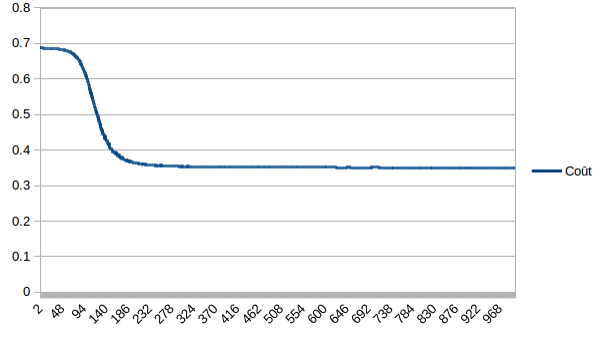
\includegraphics[scale=0.6]{images/xor_cost_function.png}
\caption{fonction de coût bloquée dans un minimum local}
\label{xor_cout_bloque}
\end{center}
\end{figure}

Nous avons alors pu remarquer que même en modifiant différents paramètres, (valeurs initiales des poids, learning rate ou les fonctions d'activation), cela restait inefficace, et les résultats obtenus ne correspondaient pas à la fonction xor que l'on attendait (voir figure \ref{xor_non_fonctionnel}).

\begin{figure}[!h]
\begin{center}
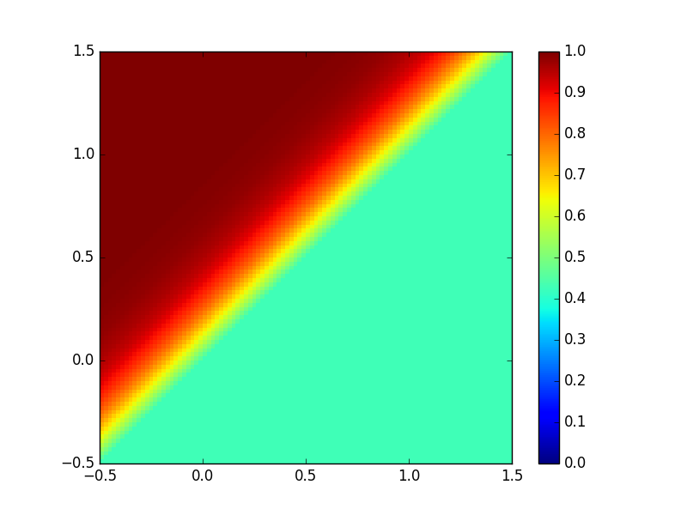
\includegraphics[scale=0.6]{images/xor_non_fonctionnel.png}
\caption{XOR bloqué dans un minimum local}
\label{xor_non_fonctionnel}
\end{center}
\end{figure}

Nous sommes alors passés sur une seconde architecture avec cette fois quatre neurones dans la couche intermédiaire cachée. On obtient cette fois de très bons résultats comme celui de la figure \ref{xor_relu_2_4}.

\begin{figure}[!h]
\begin{center}
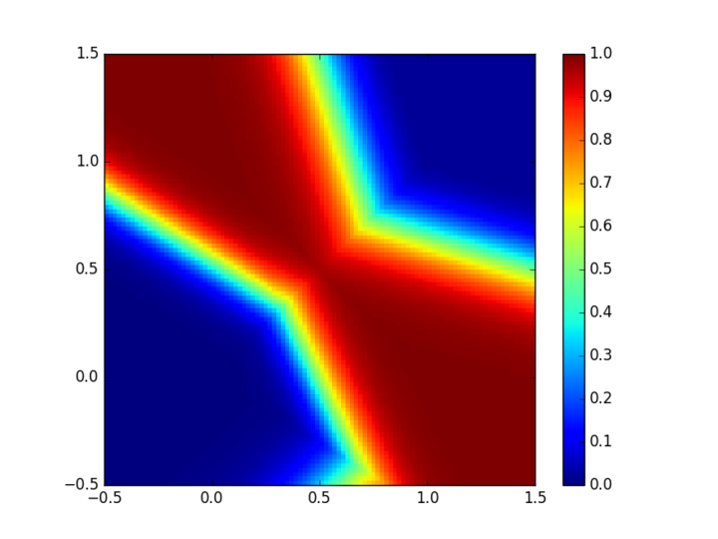
\includegraphics[scale=0.6]{images/xor_relu_2_4.png}
\caption{2 couches cachées de 4 neurones-ReLu}
\label{xor_relu_2_4}
\end{center}
\end{figure}

On peut remarquer avec cette présentation des résultats que le réseau de neurones renvoie les bonnes réponses du XOR pour les entrées définies pour l'entrainement. Pour toutes les autres valeurs,  le réseau "interprète" alors avec son apprentissage. On peut remarquer que cette interprétation varie selon la fonction d'activation. Ainsi pour la tangente hyperbolique les zones définies sont beaucoup plus courbées que pour la ReLu. On peut lier cela avec les représentations graphiques de ces fonctions. En effet la Relu est en fait deux demi-droites alors que la tangente hyperbolique a une courbe représentative beaucoup plus "arrondie".

L'apprentissage s'est donc bien réalisé pour le XOR, les résultats obtenus sont prometteurs pour la suite. Nous avons alors décidé de faire fonctionner l'algorithme sur les données MNIST.

MNIST est une base de données de chiffres écrits à la main réalisée par Yann Lecun. Cette base de donnée est constituée d'un ensemble de données d'apprentissage de 60.000 exemples et un ensemble de test constitué de 10.000 exemple. L'intersection de ces deux ensembles est nulle. Chaque exemple est donc une image d'une taille fixe d'un chiffre écrit à la main, centré. Le but est donc que notre algorithme puisse reconnaître les chiffres écrits.

Nous avons réalisé un premier apprentissage des données MNIST sur un réseau sans couche cachée totalement connecté (fully connected). Ce réseau dispose d'une entrée par pixel des images et de dix sorties, une par chiffre. Chaque entrée associe au pixel une valeur entre 0 et 255 correspond à la nuance de gris du pixel (du blanc au noir). Un premier apprentissage est réalisé sur le réseau avec un calcul du gradient moyenné sur des batchs de 128 exemples. On calcule alors la précision du réseau de neurones sur l'ensemble complet d'apprentissage ainsi que sur l'ensemble de test tous les 2.000 exemples.

\begin{figure}[!h]
\begin{center}
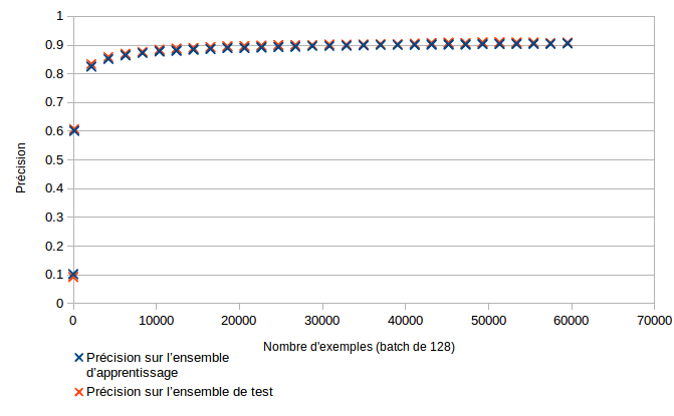
\includegraphics[scale=0.5]{images/mnist_apprentissage_128.png}
\caption{Précision en fonction du nombre d'exemples appris}
\label{mnist_apprentissage_128}
\end{center}
\end{figure}

On peut remarquer sur ces premiers résultats, que la précision progresse très vite avant de plafonner autour des 90\% dès les 10.000 exemples utilisés. Nous avons obtenu une précision maximale de 90.83\% sur cette architecture neuronale, très simpliste. Une précision plus importante pourrait être obtenue en ajoutant au moins une couche cachée au réseau. Cependant, le temps d'exécution avec cette première architecture (21.565 secondes soit plus de 6 heures), nous a montré que cela serait impossible avec de réaliser un apprentissage en un temps raisonnable avec des architectures plus compliquées.
\label{resultat_premiere_implementation}


\section{Conclusion}
Cette première implémentation intuitive permet ainsi d'obtenir des résultats très satisfaisants, allant jusqu'à 90\% de réussite sur le problème de	 MNIST. De plus, elle met en évidence le fonctionnement d'un réseau de neurones. Cependant, on remarque que les calculs ne sont pas du tout optimisés. Cela explique que le temps d'exécution devient rapidement très long. Dans l'exemple de l'application à l'ensemble de données MNIST, entraîner plusieurs fois le réseau sur l'ensemble d'apprentissage permettrait d'obtenir de bien meilleurs résultats, mais cela prendrait alors beaucoup trop de temps pour être véritablement envisageable.
Afin d'améliorer le temps de calcul et d'optimiser l'algorithme, nous nous sommes intéressés à une nouvelle approche des réseaux de neurones basée sur les graphes de calculs.

\chapter{Graphe de calculs}

\section{Motivations}

Nous avons vu précédemment que l'architecture du réseau de neurones peut être lourde autant du point de vue modélisation que du point de vue calcul. Pour motiver l'apparition des graphes de calcul prenons l'exemple d'un réseau de neurones à $m$ entrées, une couche cachée de $n$ neurones et $p$ sorties. Tous les neurones ont pour fonction d'activation une sigmoïde $\sigma$. Un tel réseau est représenté sur la figure \ref{reseau_3_5_3}.

\begin{figure}
\begin{center}
\begin{tabular}{c}
\begin{tikzpicture}[scale=0.5, line cap=round,line join=round,>=triangle 45,x=1.0cm,y=1.0cm]
\clip(-3.05,-9.53) rectangle (18.64,6.43);
\draw(2,2) circle (1cm);
\draw(2,-1) circle (1cm);
\draw(2,-4) circle (1cm);
\draw(10,2) circle (1cm);
\draw(10,-1) circle (1cm);
\draw(10,-4) circle (1cm);
\draw(6,2) circle (1cm);
\draw(6,-1) circle (1cm);
\draw(6,-4) circle (1cm);
\draw(6,5) circle (1cm);
\draw(6,-7) circle (1cm);
\draw [->] (3,2) -- (5,5);
\draw [->] (3,2) -- (5,2);
\draw [->] (3,2) -- (5,-1);
\draw [->] (3,-1) -- (5,5);
\draw [->] (3,-1) -- (5,2);
\draw [->] (3,-1) -- (5,-1);
\draw [->] (7,2) -- (9,2);
\draw [->] (7,2) -- (9,-1);
\draw [->] (7,-1) -- (9,2);
\draw [->] (7,-1) -- (9,-1);
\draw [->] (3,2) -- (5,-4);
\draw [->] (3,-1) -- (5,-4);
\draw [->] (3,-1) -- (5,-7);
\draw [->] (7,-4) -- (9,-4);
\draw [->] (7,-4) -- (9,-1);
\draw [->] (7,-4) -- (9,2);
\draw [->] (7,2) -- (9,-4);
\draw [->] (7,-1) -- (9,-4);
\draw [->] (7,-7) -- (9,-4);
\draw [->] (7,-7) -- (9,-1);
\draw [->] (7,-7) -- (9,2);
\draw [->] (7,5) -- (9,2);
\draw [->] (3,-4) -- (5,-7);
\draw [->] (7,5) -- (9,-1);
\draw [->] (7,5) -- (9,-4);
\draw [->] (3,2) -- (5,-7);
\draw [->] (3,-4) -- (5,-4);
\draw [->] (3,-4) -- (5,-1);
\draw [->] (3,-4) -- (5,2);
\draw [->] (3,-4) -- (5,5);
\draw (1.5,2.5) node[anchor=north west] {$ x_1 $};
\draw (1.5,-0.5) node[anchor=north west] {$ x_2 $};
\draw (1.5,-3.5) node[anchor=north west] {$ x_3 $};
\draw (9.5,2.5) node[anchor=north west] {$ y_1 $};
\draw (9.5,-0.5) node[anchor=north west] {$ y_2 $};
\draw (9.5,-3.5) node[anchor=north west] {$ y_3 $};
\end{tikzpicture} \\
\begin{tikzpicture}[scale=0.5, line cap=round,line join=round,>=triangle 45,x=1.0cm,y=1.0cm]
\draw(1,0) circle (1cm);
\draw(5,0) circle (1cm);
\draw(5,4) circle (1cm);
\draw(9,0) circle (1cm);
\draw(13,0) circle (1cm);
\draw(13,4) circle (1cm);
\draw(17,0) circle (1cm);
\draw [->] (5,3) -- (5,1);
\draw [->] (2,0) -- (4,0);
\draw [->] (6,0) -- (8,0);
\draw [->] (10,0) -- (12,0);
\draw [->] (13,3) -- (13,1);
\draw [->] (14,0) -- (16,0);
\draw [->] (18,0) -- (20,0);
\draw (0.5,0.4) node[anchor=north west] {$ x $};
\draw (4.4,4.7) node[anchor=north west] {$ W_1 $};
\draw (12.4,4.7) node[anchor=north west] {$ W_2 $};
\draw (4.5,0.5) node[anchor=north west] {$ \times $};
\draw (8.6,0.4) node[anchor=north west] {$ \sigma $};
\draw (12.5,0.5) node[anchor=north west] {$ \times $};
\draw (16.6,0.4) node[anchor=north west] {$ \sigma $};
\draw (18.5,1.2) node[anchor=north west] {$ y $};
\end{tikzpicture} \\
\end{tabular}
\end{center}
\caption{Réseau de neurones à 3 entrées, 5 neurones cachés et 3 neurones de sorties (en haut). La représentation équivalente en utilisant un graphe de calculs (en bas).}
\label{reseau_3_5_3}
\end{figure}

Nous pourrions modéliser ce réseau de neurone en définissant $n+p$ neurones ayant chacun son vecteur poids mais une façon équivalente de modéliser ce système est de rassembler les poids des deux couches dans deux matrices $W_1 \in \mathbb{R}^{m \times n}$ et $W_2 \in \mathbb{R}^{n \times p}$. En notant $x \in \mathbb{R}^m$ le vecteur ligne des entrées du réseau, on a alors que la sortie est :
\begin{equation}
y = \sigma(\sigma(xW_1)W_2)
\label{eq_3_5_3}
\end{equation}
où la fonction $\sigma$ s'applique terme à terme. 

Sur la figure \ref{reseau_3_5_3}, en bas, est représentée cette formule de manière graphique. Un tel graphe sera appelé graphe de calculs.

Cette modélisation matricielle a de nombreux avantages. Tout d'abord, elle est plus compacte et simple à manipuler et à visualiser. Puis, elle a un avantage certain pour notre implémentation en Python car elle permet d'utiliser pleinement la librairie d'algèbre linéaire \texttt{numpy} ce qui accélerera grandement les calculs. Enfin, il est facile d'étendre la formule précédente au calcul de la sortie de plusieurs vecteurs d'entrées. En effet si $X \in \mathbb{R}^{N \times m}$ est une matrice contenant $N$ vecteurs d'entrées alors la sortie du réseau s'écrit :
$$Y = \sigma(\sigma(XW_1)W_2)$$

On aurait donc envie de s'affranchir de la structure du neurone pour seulement modéliser les opérations mathématiques effectuées par le réseau.

\section{Définitions}

\begin{definition}[Graphe de calcul]
Un graphe de calcul est un graphe représentant une fonction mathématique. Un n\oe{}ud de ce graphe représente soit une variable, des poids ou une opération mathématique. Formellement, nous noterons $\mathcal{G}(V, A, V_{var}, (V_{op}, f), (V_{poids}, \theta))$ le graphe $\mathcal{G}$ dont les n\oe{}uds sont $V$, les arêtes $A$, $V_{var} \subset V$ les n\oe{}uds réprésentant une variable, $V_{op} \subset V$ ceux représentant une opération et $f$ les opérations en question, et $V_{poids} \subset V$ ceux représentant des poids et $\theta$ les poids associés.
\end{definition}

Dans cette définition, nous considérons les variables comme les arguments du graphe de calculs. En ce qui concerne, les réseaux de neurones, les entrées seront un n\oe{}ud représentant une variable. Les poids sont les paramètres de la fonction. Ce seront les poids des neurones par exemple. Nous n'imposons pour l'instant aucune limite aux opérations mathématiques pouvant être effectuées au sein des graphes de calculs.

Dans le graphe de calculs de la figure \ref{reseau_3_5_3}, le n\oe{}ud $x$ est une variable, les n\oe{}uds $W_1$ et $W_2$ sont des poids et les deux n\oe{}uds $\sigma$ représente l'opération sigmoïde appliquée terme à terme. Nous remarquerons que la sortie $y$ n'est pas explicitée par un n\oe{}ud. 

Les graphes de calculs offrent une très grande liberté. Il est possible de représenter avec ceux-ci une classe de fonctions bien plus grandes qu'avec des réseaux de neurones classiques.

Écrivons dès maintenant, l'algorithme de propagation. Afin de pouvoir être concis, nous devons ajouter des notations. Nous noterons l'arc allant de la sortie $k$ du n\oe{}ud $n_i$ vers l'entrée $l$ du n\oe{}ud $n_j$ comme un quadruplet $(n_i, k, n_j, l)$. De plus, nous noterons $in(n)$ le nombre d'entrées du n\oe{}ud $n$ et $out(n)$ le nombres de sorties du n\oe{}ud $n$.

\begin{algorithm} 
\begin{algorithmic}
\Procedure{$evaluer\_graphe$}{$\mathcal{G}(V, A, V_{var}, (V_{op}, f), (V_{poids}, \theta)), x$}
\Function{$evaluer\_noeud$}{$n_j$}
	\If{$déjàCalculé[j]$ est $faux$}
		\State // 1. On récupère les valeurs des entrées.
		\State $t \leftarrow (evaluer\_noeud(i)_k, (n_i, k, l)\text{ tel que }(n_i, k, n_j, l) \in A)$
		\State // 2. On calcule les valeurs de sortie.
		\State $y_j \leftarrow f_j(t)$
		\State // 3. On mémoïse.
		\State $déjàCalculé[j] \leftarrow vrai$
	\EndIf
	\State \Return $y_j$
\EndFunction

\State Initialiser un tableau $dejaCalculé$ de longueur $|V|$ à $faux$.
\For{$n_i \in V_{var}$}
	\State $y_i \leftarrow x_i$
	\State $déjàCalculé[i] \leftarrow vrai$ 
\EndFor
\For{$n_j \in V$}
	\State $evaluer\_noeud(n_j)$ 
\EndFor
\EndProcedure
\end{algorithmic}
\caption{Algorithme d'évaluation d'un graphe de calculs.}
\label{propagation_memoisation}
\end{algorithm}

Nous remarquons que l'algorithme de propagation est très similaire à celui décrit pour les réseaux de neurones. En effet, les graphes de calculs en sont une généralisation.

Nous avons ainsi modéliser nos réseaux de manière plus efficace. Il reste cependant un problème à résoudre. Notre objectif est d'optimiser les paramètres de notre fonction. Pour cela, nous avons besoin de calculer la dérivée du coût $E$ par rapport aux poids avant de pouvoir utiliser l'algorithme de la descente du gradient.

\section{Dérivation automatique}

Afin de réaliser cela, nos n\oe{}uds représentant des opérations mathématiques ne seront pas seulement responsable de calculer une sortie mais aussi de propager le gradient. En effet prenons un n\oe{}ud représent une opération mathématique $f$ à $m$ entrées $x_1, ..., x_m$ et à $n$ sorties $y_1, ..., y_n$. La règle de la chaine, nous permet d'exprimer la dérivée du coût par rapport aux entrées en fonction du coût par rapport aux sorties du n\oe{}ud. En effet, on a :
\begin{equation}
\forall i \in \{1, ...,  m\}, \frac{\partial E}{\partial x_i} = \sum_{j=1}^{n}{\frac{\partial y_j}{\partial x_i}\frac{\partial E}{\partial y_j}} = \sum_{j=1}^{n}{\frac{\partial f_j}{\partial x_i}(x)\frac{\partial E}{\partial y_j}}
\label{retropropagation_graphe}
\end{equation}

Rappelons que si $x_i \in \mathbb{R}^p$ et $y_j \in \mathbb{R}^q$ alors $\frac{\partial E}{\partial y_j} \in \mathbb{R}^q$ et $\frac{\partial y_j}{\partial x_i} = (\frac{\partial y_{j,l}}{\partial x_{i, k}})_{k, l} \in \mathbb{R}^{p \times q}$.

La formule \ref{retropropagation_graphe} nous permet de décrire un algorithme de rétropropagation du gradient très similaire à celui des réseaux de neurones :

\begin{algorithm} 
\begin{algorithmic}
\Procedure{$retropropager\_gradient$}{$\mathcal{G}(V, A, V_{var}, (V_{op}, f), (V_{poids}, \theta)), x, y$}
\Function{$calculer\_gradient$}{$n_i$}
	\If{$déjàCalculé[i]$ est $faux$}
		\State // 1. Pour chaque sortie, on récupère la dérivée du coût par rapport à celle-ci.
		\For{k dans $\{1, ..., out(n_i)\}$}
			\State $\frac{\partial E}{\partial y_{i, k}} \leftarrow \sum\limits_{(n_j, l)\text{ tel que }(n_i, k, n_j, l) \in A}{calculer\_gradient(n_j)_l}$
		\EndFor
		\State // 2. Pour chaque entrée, on calcule la dérivée du coût par rapport à celle-ci.
		\For{l dans $\{1, ..., in(n_i)\}$}
			\State $\frac{\partial E}{\partial x_{i, l}} \leftarrow \sum\limits_{k \in \{1, ..., out(n_i) \}}{\frac{\partial f_{i, k}}{\partial x_{i, l}}(x)\frac{\partial E}{\partial y_{i, k}}}$
		\EndFor
		\State // 3. On mémoïse.
		\State $déjàCalculé[i] \leftarrow vrai$
	\EndIf
	\State \Return $\frac{\partial E}{\partial x_j}$
\EndFunction

\State Appeler $evaluer\_graphe(\mathcal{N}(V, A, V_{in}, V_{out}, f), x)$ et récupérer les entrées et sorties de chaque noeud
\State Initialiser un tableau $dejaCalculé$ de longueur $|V|$ à $faux$.
\For{$n_i \in V_{out}$}
	\State Calculer $\frac{\partial E}{\partial y_i}$
	\State $déjàCalculé_i \leftarrow vrai$ 
\EndFor
\For{$n_i \in V$}
	\State $calculer\_gradient(n_i)$ 
\EndFor
\EndProcedure
\end{algorithmic} 
\caption{Algorithme de rétropropagation du gradient dans un graphe de calculs.}
\label{propagation_memoisation2}
\end{algorithm}

\section{N\oe{}uds}

Maintenant que les graphes de calculs ont été présentés de manière théorique, nous allons dans la suite présenter de manière plus pratique comment nous les avons implémentés.

\subsection{La classe Node}

Un n\oe{}ud aura deux missions : calculer sa sortie et rétropropager le gradient. Nous représentions ces deux opérations sur la figure \ref{node}.

\begin{figure}
\begin{center}
\begin{tabular}{cc}
\begin{tikzpicture}[line cap=round,line join=round,>=triangle 45,x=1.0cm,y=1.0cm]
\draw(1,2) circle (1cm);
\draw [->] (-1.5,2) -- (0,2);
\draw [->] (-1.5,3) -- (0.13,2.5);
\draw [->] (-1.5,1) -- (0.13,1.51);
\draw [->] (1.86,2.51) -- (3.5,3);
\draw [->] (2,2) -- (3.5,2);
\draw [->] (1.87,1.5) -- (3.5,1);
\draw [->] (3,2.85) -- (3.4,3.35);
\draw [->] (3,2.85) -- (3.49,2.68);
\draw [->] (3,2) -- (3.58,2.3);
\draw [->] (3,2) -- (3.53,1.74);
\draw [->] (3.01,1.15) -- (3.33,0.7);
\draw [->] (3.01,1.15) -- (3.55,1.34);
\draw (-0.85,3.1) node[anchor=north west] {$ x_1 $};
\draw (-0.85,2.4) node[anchor=north west] {$ x_2 $};
\draw (-0.85,1.7) node[anchor=north west] {$ x_3 $};
\draw (2.2,3.1) node[anchor=north west] {$ y_1 $};
\draw (2.2,2.4) node[anchor=north west] {$ y_2 $};
\draw (2.2,1.7) node[anchor=north west] {$ y_3 $};
\end{tikzpicture} & \begin{tikzpicture}[line cap=round,line join=round,>=triangle 45,x=1.0cm,y=1.0cm]
\draw(1,2) circle (1cm);
\draw [->] (3.5,3) -- (1.86,2.51);
\draw [->] (3.5,2) -- (2,2);
\draw [->] (3.5,1) -- (1.87,1.5);
\draw (-0.9,3.4) node[anchor=north west] {$ \frac{\partial E}{\partial x_1} $};
\draw (-0.9,2.6) node[anchor=north west] {$ \frac{\partial E}{\partial x_2} $};
\draw (-0.9,1.9) node[anchor=north west] {$ \frac{\partial E}{\partial x_3} $};
\draw (2.3,3.4) node[anchor=north west] {$ \frac{\partial E}{\partial y_1} $};
\draw (2.3,2.6) node[anchor=north west] {$ \frac{\partial E}{\partial y_2} $};
\draw (2.3,1.9) node[anchor=north west] {$ \frac{\partial E}{\partial y_3} $};
\draw [->] (0.13,2.5) -- (-1.5,3);
\draw [->] (0,2) -- (-1.5,2);
\draw [->] (0.13,1.51) -- (-1.5,1);
\draw [->] (3.4,3.35) -- (3,2.85);
\draw [->] (3.49,2.68) -- (3,2.85);
\draw [->] (3.58,2.3) -- (3,2);
\draw [->] (3.53,1.74) -- (3,2);
\draw [->] (3.55,1.34) -- (3.01,1.15);
\draw [->] (3.33,0.7) -- (3.01,1.15);
\draw [->] (3.5,3) -- (3,2.85);
\draw [->] (3.5,2) -- (3,2);
\draw [->] (3.5,1) -- (3.01,1.15);
\end{tikzpicture} \\
\end{tabular}
\end{center}
\caption{Représentation de la propagation (à gauche) et de la rétropropagation (à droite) au sein d'un n\oe{}ud.}
\label{node}
\end{figure}

Lors de la propagation, un n\oe{}ud demande ses entrées à ses parents puis calcule sa sortie et la mémoïse. De façon analogue, lors de la rétropropagation, un n\oe{}ud demande à chacun de ses enfants le gradient par rapport à la sortie qu'ils utilisent puis s'en sert pour calculer le gradient par rapport à ses entrées et mémoïse
.

\subsection{Les opérations mathématiques}

Dans cette sous-section, nous allons décrire les symboles ainsi que les formules des n\oe{}uds que nous avons implémentés. \label{nodes}

Nous commençons d'abord par décrire les n\oe{}uds à une entrée et une sortie :

\begin{center}
\begin{tabular}{|m{3.5cm}|m{2.7cm}|m{4.5cm}|}
\hline
\begin{center}Symbole\end{center} & \begin{center}Formule de propagation\end{center} & \begin{center}Formule de rétropropagation\end{center} \\
\hline
\begin{center}\begin{tikzpicture}[line cap=round,line join=round,>=triangle 45,x=1.0cm,y=1.0cm, scale=0.6]
\draw(3,0) circle (1cm);
\draw [->] (0,0) -- (2,0);
\draw [->] (4,0) -- (6,0);
\draw (0.86,0.64) node[anchor=north west] {$ x $};
\draw (4.86,0.66) node[anchor=north west] {$ y $};
\draw (2.6,0.4) node[anchor=north west] {$ \sigma $};
\end{tikzpicture}\end{center} & \begin{center}$\sigma(x) = \frac{1}{1 + \exp(-x)}$\end{center} & \begin{center}$\frac{\partial E}{\partial y} \odot y \odot (1 - y)$\end{center} \\
\hline
\begin{center}\begin{tikzpicture}[line cap=round,line join=round,>=triangle 45,x=1.0cm,y=1.0cm, scale=0.6]
\draw(3,0) circle (1cm);
\draw [->] (0,0) -- (2,0);
\draw [->] (4,0) -- (6,0);
\draw (0.86,0.64) node[anchor=north west] {$ x $};
\draw (4.86,0.66) node[anchor=north west] {$ y $};
\draw (2.3,0.4) node[anchor=north west] {$ \tanh $};
\end{tikzpicture}\end{center} & \begin{center}$\tanh(x)$\end{center} & \begin{center}$\frac{\partial E}{\partial y} \odot (1 - y \odot y)$\end{center} \\ 
\hline
\begin{center}\begin{tikzpicture}[line cap=round,line join=round,>=triangle 45,x=1.0cm,y=1.0cm, scale=0.6]
\draw(3,0) circle (1cm);
\draw [->] (0,0) -- (2,0);
\draw [->] (4,0) -- (6,0);
\draw (0.86,0.64) node[anchor=north west] {$ x $};
\draw (4.86,0.66) node[anchor=north west] {$ y $};
\draw (2.05,0.4) node[anchor=north west] {$ ReLU $};
\end{tikzpicture}\end{center} & \begin{center}$ReLU(x)$\end{center} & \begin{center}$\frac{\partial E}{\partial y} \odot (\mathds{1}_{x_{i,j} \geq 0})_{i,j}$\end{center} \\ 
\hline
\begin{center}\begin{tikzpicture}[line cap=round,line join=round,>=triangle 45,x=1.0cm,y=1.0cm, scale=0.6]
\draw(3,0) circle (1cm);
\draw [->] (0,0) -- (2,0);
\draw [->] (4,0) -- (6,0);
\draw (0.86,0.64) node[anchor=north west] {$ x $};
\draw (4.86,0.66) node[anchor=north west] {$ y $};
\draw (1.75,0.4) node[anchor=north west] {\begin{small}$ softmax $\end{small}};
\end{tikzpicture}\end{center} & \begin{center}$softmax(x)$\end{center} & \begin{center}$\left(\sum_{k = 1}^{n}{y_{i,j}(\delta_{j,k} - y_{i,k})\frac{\partial E}{\partial y_{i, k}}}\right)_{i,j}$\end{center} \\ 
\hline
\begin{center}\begin{tikzpicture}[line cap=round,line join=round,>=triangle 45,x=1.0cm,y=1.0cm, scale=0.6]
\draw(3,0) circle (1cm);
\draw [->] (0,0) -- (2,0);
\draw [->] (4,0) -- (6,0);
\draw (0.86,0.64) node[anchor=north west] {$ x $};
\draw (4.86,0.66) node[anchor=north west] {$ y $};
\draw (2.4,0.5) node[anchor=north west] {$ ||.||_2^2 $};
\end{tikzpicture}\end{center} & \begin{center}$||x||_2^2$\end{center} & \begin{center}$2\frac{\partial E}{\partial y}x$\end{center} \\ 
\hline
\begin{center}\begin{tikzpicture}[line cap=round,line join=round,>=triangle 45,x=1.0cm,y=1.0cm, scale=0.6]
\draw(3,0) circle (1cm);
\draw [->] (0,0) -- (2,0);
\draw [->] (4,0) -- (6,0);
\draw (0.86,0.64) node[anchor=north west] {$ x $};
\draw (4.86,0.66) node[anchor=north west] {$ y $};
\draw (2.4,0.5) node[anchor=north west] {$ 1|. $};
\end{tikzpicture}\end{center} & \begin{center}$1|x = \begin{pmatrix}1 & x\end{pmatrix}$\end{center} & \begin{center}$(\frac{\partial E}{\partial y}_{i, j})_{i \in \{2, ..., m+1\}, j \in \{1, ..., n\}}$\end{center} \\ 
\hline
\end{tabular}
\end{center}

Puis ceux à deux entrées et une sortie :

\begin{center}
\begin{tabular}{|m{4cm}|m{3.cm}|m{3.cm}|}
\hline
\begin{center}Symbole\end{center} & \begin{center}Formule de propagation\end{center} & \begin{center}Formule de rétropropagation\end{center} \\
\hline
\begin{center}\begin{tikzpicture}[line cap=round,line join=round,>=triangle 45,x=1.0cm,y=1.0cm, scale=0.6]
\draw(3,0) circle (1cm);
\draw [->] (0,0.6) -- (2.02,0.2);
\draw [->] (4,0) -- (6,0);
\draw (4.86,0.65) node[anchor=north west] {$ y $};
\draw (2.6,0.4) node[anchor=north west] {$ + $};
\draw [->] (0,-0.6) -- (2.02,-0.2);
\draw (0.85,1.06) node[anchor=north west] {$ x_1 $};
\draw (0.87,-0.39) node[anchor=north west] {$ x_2 $};
\end{tikzpicture}\end{center} & \begin{center}$x_1 + x_2$\end{center} & \begin{center}$(\frac{\partial E}{\partial y}, \frac{\partial E}{\partial y})$\end{center} \\
\hline
\begin{center}\begin{tikzpicture}[line cap=round,line join=round,>=triangle 45,x=1.0cm,y=1.0cm, scale=0.6]
\draw(3,0) circle (1cm);
\draw [->] (0,0.6) -- (2.02,0.2);
\draw [->] (4,0) -- (6,0);
\draw (4.86,0.65) node[anchor=north west] {$ y $};
\draw (2.6,0.4) node[anchor=north west] {$ - $};
\draw [->] (0,-0.6) -- (2.02,-0.2);
\draw (0.85,1.06) node[anchor=north west] {$ x_1 $};
\draw (0.87,-0.39) node[anchor=north west] {$ x_2 $};
\end{tikzpicture}\end{center} & \begin{center}$x_1 - x_2$\end{center} & \begin{center}$(\frac{\partial E}{\partial y}, -\frac{\partial E}{\partial y})$\end{center} \\
\hline
\begin{center}\begin{tikzpicture}[line cap=round,line join=round,>=triangle 45,x=1.0cm,y=1.0cm, scale=0.6]
\draw(3,0) circle (1cm);
\draw [->] (0,0.6) -- (2.02,0.2);
\draw [->] (4,0) -- (6,0);
\draw (4.86,0.65) node[anchor=north west] {$ y $};
\draw (2.6,0.4) node[anchor=north west] {$ \times $};
\draw [->] (0,-0.6) -- (2.02,-0.2);
\draw (0.85,1.06) node[anchor=north west] {$ x_1 $};
\draw (0.87,-0.39) node[anchor=north west] {$ x_2 $};
\end{tikzpicture}\end{center} & \begin{center}$x_1 \times x_2$\end{center} & \begin{center}$(\frac{\partial E}{\partial y}x_2^T, x_1^T\frac{\partial E}{\partial y})$\end{center} \\
\hline
\begin{center}\begin{tikzpicture}[line cap=round,line join=round,>=triangle 45,x=1.0cm,y=1.0cm, scale=0.6]
\draw(3,0) circle (1cm);
\draw [->] (0,0.6) -- (2.02,0.2);
\draw [->] (4,0) -- (6,0);
\draw (4.86,0.65) node[anchor=north west] {$ y $};
\draw (2.6,0.4) node[anchor=north west] {$ \odot $};
\draw [->] (0,-0.6) -- (2.02,-0.2);
\draw (0.85,1.06) node[anchor=north west] {$ x_1 $};
\draw (0.87,-0.39) node[anchor=north west] {$ x_2 $};
\end{tikzpicture}\end{center} & \begin{center}$x_1 \odot x_2$\end{center} & \begin{center}$(\frac{\partial E}{\partial y} \odot x_2, \frac{\partial E}{\partial y} \odot x_1)$\end{center} \\
\hline
\begin{center}\begin{tikzpicture}[line cap=round,line join=round,>=triangle 45,x=1.0cm,y=1.0cm, scale=0.6]
\draw(3,0) circle (1cm);
\draw [->] (0,0.6) -- (2.02,0.2);
\draw [->] (4,0) -- (6,0);
\draw (4.86,0.65) node[anchor=north west] {$ y $};
\draw (2.7,0.4) node[anchor=north west] {$ | $};
\draw [->] (0,-0.6) -- (2.02,-0.2);
\draw (0.85,1.06) node[anchor=north west] {$ x_1 $};
\draw (0.87,-0.39) node[anchor=north west] {$ x_2 $};
\end{tikzpicture}\end{center} & \begin{center}$x_1|x_2 = \begin{pmatrix}x_1 & x_2\end{pmatrix}$\end{center} & \begin{center}$ $\end{center} \\
\hline
\begin{center}\begin{tikzpicture}[line cap=round,line join=round,>=triangle 45,x=1.0cm,y=1.0cm, scale=0.6]
\draw(3,0) circle (1cm);
\draw [->] (0,0.6) -- (2.02,0.2);
\draw [->] (4,0) -- (6,0);
\draw (4.86,0.65) node[anchor=north west] {$ y $};
\draw (1.8,0.6) node[anchor=north west] {\begin{small}$ sigmoid $\end{small}};
\draw (2.3,0.05) node[anchor=north west] {\begin{small}$ CE $\end{small}};
\draw [->] (0,-0.6) -- (2.02,-0.2);
\draw (0.85,1.06) node[anchor=north west] {$ x_1 $};
\draw (0.87,-0.39) node[anchor=north west] {$ x_2 $};
\end{tikzpicture}\end{center} & \begin{center}$sigmoidCE(x_1, x_2)$\end{center} & \begin{center}$ $\end{center} \\
\hline
\begin{center}\begin{tikzpicture}[line cap=round,line join=round,>=triangle 45,x=1.0cm,y=1.0cm, scale=0.6]
\draw(3,0) circle (1cm);
\draw [->] (0,0.6) -- (2.02,0.2);
\draw [->] (4,0) -- (6,0);
\draw (4.86,0.65) node[anchor=north west] {$ y $};
\draw (1.75,0.6) node[anchor=north west] {\begin{small}$ softmax $\end{small}};
\draw (2.3,0.05) node[anchor=north west] {\begin{small}$ CE $\end{small}};
\draw [->] (0,-0.6) -- (2.02,-0.2);
\draw (0.85,1.06) node[anchor=north west] {$ x_1 $};
\draw (0.87,-0.39) node[anchor=north west] {$ x_2 $};
\end{tikzpicture}\end{center} & \begin{center}$softmaxCE(x_1, x_2)$\end{center} & \begin{center}$ $\end{center} \\
\hline
\end{tabular}
\end{center}

\subsection{Dérivation matricielle}

Afin d'avoir des performances correctes en utilistant Python, nous avions comme contrainte d'optimiser notre utilisation de la bibliothèque \texttt{numpy}. Pour cela, il faut privilégier les appels à cette librairie qui exécute du code compilé plutôt que d'écrire nous-même les calculs en Python qui seraient interprétés et donc exécutés bien plus lentement.

Or afin d'utiliser la descente du gradient, il faut calculer la dérivée du coût qui est scalaire par rapport aux poids qui sont stockés dans une matrice. Le moyen le plus efficace  de calculer cette quantité est d'obtenir une formule faisant intervenir directement des matrices.

Au début du projet, nous n'étions pas très à l'aise avec les dérivées matricielles. De plus, nous n'avons pas trouvé dans la littérature de document expliquant clairement le concept et donnant un formulaire utile pour les réseaux de neurones. Dans cette sous-section nous allons donc rappeler le concept et les notations. Puis nous démontrerons les formules énoncées ci-dessus pour expliciter la méthode permettant de d'obtenir de telles formules.

\begin{definition}[Dérivée tensorielle]
Soit une fonction $f : \mathbb{R}^{m_1 \times ... \times m_p} \rightarrow \mathbb{R}^{n_1 \times ... \times n_q}$. Nous appelerons dérivée tensorielle de f en $x$ notée $\frac{\partial f}{\partial x}(x)$, le tenseur $(\frac{\partial f_{j_1, ..., j_q}}{\partial x_{i_1, ..., i_p}}(x))_{i_1, ..., i_p, j_1, ..., j_q} \in  \mathbb{R}^{m_1 \times ... \times m_p \times n_1 \times ... \times n_q}$ 
\end{definition}

Dans notre cas, nous calculerons toujours les dérivées d'une fonction à valeur dans $\mathbb{R}$, le coût et à arguments matriciels, les poids. Nous utiliserons donc le cas particulier suivant.

\begin{definition}[Dérivée matricielle]
Soit une fonction $f : \mathbb{R}^{m \times n} \rightarrow \mathbb{R}$. Nous appelerons dérivée matricielle de f en $x$ notée $\frac{\partial f}{\partial x}(x)$, la matrice $(\frac{\partial f}{\partial x_{i, j}}(x))_{i, j} \in  \mathbb{R}^{m \times n}$ 
\end{definition}

\begin{remark}
Dans la suite du document, si $y = f(x)$, nous noterons $\frac{\partial f}{\partial x}(x)$, la dérivée de $f$ par rapport à $x$ évaluée en $x$, $\frac{\partial y}{\partial x}$.
\end{remark}

\begin{remark}
Nous avons choisi la convention $\frac{\partial f}{\partial x}(x) = (\frac{\partial f}{\partial x_{i, j}}(x))_{i, j}$ cependant il est possible que d'autres auteurs utilisent la convention $\frac{\partial f}{\partial x}(x) = (\frac{\partial f}{\partial x_{i, j}}(x))_{j, i}$. Les deux conventions ont des avantages et des inconvénients, aucune ne fait a priori consensus. Nous avons choisi la première car la dérivée a la même taille que l'argument. Par conséquent pour la descente du gradient, nous pouvons simplement écrire :
$$
w(t+1) = w(t) - \eta \frac{\partial E}{\partial w} 
$$
ce qui est fort élégant.

Nous donnerons tous les résultats en suivant notre convention. Cependant, ce n'est pas une fatalité puisqu'il suffit de transposer les résultats pour les obtenir selon l'autre convention.
\end{remark}

Donnons dès à présent, le résultat qui va nous être le plus utile, la règle de la chaine en version matricielle.

\begin{proposition}[Règle de la chaine]
Soit $f : \mathbb{R}^{m \times n} \rightarrow \mathbb{R}^{p \times q}$, $g : \mathbb{R}^{p \times q} \rightarrow \mathbb{R}$, et $x \in \mathbb{R}^{m \times n}$. Notons $y = f(x)$ et $z = g(y)$ pour simplifier, on a alors :
$$
\forall i \in \{1, ..., m\}, j \in \{1, ..., n\}, (\frac{\partial z}{\partial x})_{i, j} = \sum_{k \in \{1, ..., p\}, l \in \{1, ..., q\}}{\frac{\partial z}{\partial y_{k, l}}\frac{\partial y_{k, l}}{\partial x_{i, j}}}
$$
\end{proposition}

Nous remarquons donc que dans le cas général, il n'y a pas de formule simple permettant de calculer la dérivée. Cependant pour les opérations que nous utilisons, cette formule se simplifie.

Nous allons dans la suite démontrer toutes les formules énoncées dans la sous-section \ref{nodes}. Cette partie pourra servir d'exercices pour le lecteur voulant s'initier à la dérivation matricielle ou de mémo pour ses rédacteurs.

Afin de rester dans le cadre de l'apprentissage automatique, nous appelerons comme dans les sections précédentes $E$ notre fonction à valeurs dans $\mathbb{R}$.

La démarche pour dériver chaque formule sera toujours la même :
\begin{enumerate}
\item On exprime $\frac{\partial E}{\partial x_{i, j}}$ en fonction des $(\frac{\partial E}{\partial y_{k, l}})_{k, l}$ en utilisant la règle de la chaine énoncée ci-dessus. On ne manipule ici que des dérivées scalaires, on peut donc utiliser toutes les opérations habituelles sans prendre de précautions.
\item On reconnait dans l'expression obtenue de $\frac{\partial E}{\partial x_{i, j}}$ une opération connue qu'il est possible d'exprimer en notation matricielle.
\end{enumerate}

\begin{proposition}
Si $y = \sigma(x)$ alors $\frac{\partial E}{\partial x} = \frac{\partial E}{\partial y} \odot y \odot (1 - y)$.
\label{derivative_sigmoid}
\end{proposition}

Afin de démontrer ce résultat, nous utiliserons le lemme suivant donnant le résultat dans le cas scalaire.

\begin{lemma}
Soit $\sigma : x \in \mathbb{R} \mapsto \frac{1}{1 + \exp(-x)}$, on a :
$$ 
\forall x \in \mathbb{R}, \sigma'(x) = \sigma(x)(1 - \sigma(x))
$$
\label{sigmoid_scalar}
\end{lemma}

\begin{proof}
Soit $x \in \mathbb{R}$, en utilisant les règles de dérivation, on a :
$$
\sigma'(x) = \frac{\exp(-x)}{(1 + \exp(-x))^2} = \frac{1}{1 + \exp(-x)}\frac{\exp(-x)}{1 + \exp(-x)}
$$
d'où :
$$
\sigma'(x) = \sigma(x)\frac{(1 + \exp(x)) - 1}{1 + \exp(-x)} =  \sigma(x)(1 - \sigma(x))
$$
\end{proof}

Nous pouvons alors démontrer la proposition \ref{derivative_sigmoid}.

\begin{proof}
L'opération $\sigma$ étant appliquée terme à terme, on a que :
$$
\forall i \in \{1, ..., m\}, j \in \{1, ..., n\}, \frac{\partial E}{\partial x_{i, j}} = \frac{\partial E}{\partial y_{i, j}}\frac{\partial y_{i, j}}{\partial x_{i, j}}
$$
Or d'après le lemme \ref{sigmoid_scalar}, $\frac{\partial y_{i, j}}{\partial x_{i, j}} = y_{i, j}(1 - y_{i, j})$. Donc :
$$
\forall i \in \{1, ..., m\}, j \in \{1, ..., n\}, \frac{\partial E}{\partial x_{i, j}} = \frac{\partial E}{\partial y_{i, j}}y_{i, j}(1 - y_{i, j})
$$
On reconnait alors des produits terme à terme et on en conclut que :
$$
\frac{\partial E}{\partial x} = \frac{\partial E}{\partial y} \odot y \odot (1 - y)
$$
\end{proof}

\begin{proposition}
Si $y = \tanh(x)$ alors $\frac{\partial E}{\partial x} = \frac{\partial E}{\partial y} \odot (1 - y \odot y)$.
\label{derivative_tanh}
\end{proposition}

Rappelons sans démonstration, le résultat bien connu sur la dérivée de $\tanh$.

\begin{lemma}
$$ 
\forall x \in \mathbb{R}, \tanh'(x) = 1 - \tanh(x)^2
$$
\label{tanh_scalar}
\end{lemma}

À l'aide de ce résultat, prouvons la proposition \ref{derivative_tanh}.

\begin{proof}
De même que pour $\sigma$, l'opération $\tanh$ étant appliquée terme à terme, on a que :
$$
\forall i \in \{1, ..., m\}, j \in \{1, ..., n\}, \frac{\partial E}{\partial x_{i, j}} = \frac{\partial E}{\partial y_{i, j}}\frac{\partial y_{i, j}}{\partial x_{i, j}}
$$
Or d'après le lemme \ref{tanh_scalar}, $\frac{\partial y_{i, j}}{\partial x_{i, j}} = 1 - y_{i, j}^2$. Donc :
$$
\forall i \in \{1, ..., m\}, j \in \{1, ..., n\}, \frac{\partial E}{\partial x_{i, j}} = \frac{\partial E}{\partial y_{i, j}}(1 - y_{i, j}^2)
$$
On reconnait alors, ici encore, des produits terme à terme et on en conclut que :
$$
\frac{\partial E}{\partial x} = \frac{\partial E}{\partial y} \odot (1 - y \odot y)
$$
\end{proof}

\begin{proposition}
Si $y = ReLU(x)$ alors $\frac{\partial E}{\partial x} = \frac{\partial E}{\partial y} \odot (\mathds{1}_{x_{i,j} \geq 0})_{i,j}$.
\end{proposition}

\begin{proposition}
Si $y = softmax(x)$ alors $\frac{\partial E}{\partial x} = \left(\sum_{k = 1}^{n}{y_{i,j}(\delta_{j,k} - y_{i,k})\frac{\partial E}{\partial y_{i, k}}}\right)_{i,j}$.
\end{proposition}

\begin{proposition}
Si $y = ||x||_2^2$ alors $\frac{\partial E}{\partial x} = 2\frac{\partial E}{\partial y}x$.
\end{proposition}

\begin{proposition}
Si $y = 1|x = \begin{pmatrix}1 & x\end{pmatrix}$ alors $\frac{\partial E}{\partial x} = (\frac{\partial E}{\partial y}_{i, j})_{i \in \{2, ..., m+1\}, j \in \{1, ..., n\}}$.
\end{proposition}

\begin{proposition}
Si $y = x_1 + x_2$ alors $\frac{\partial E}{\partial x_1} = \frac{\partial E}{\partial x_2} = \frac{\partial E}{\partial y}$.
\end{proposition}

\begin{proof}
Comme l'addition est faite terme à terme, pour tout $i \in \{1, ..., m\}, j \in \{1, ..., n\}$, $y_{i, j} = x_{1_{i, j}} + x_{2_{i, j}}$ ne dépend que de $x_{1_{i, j}}$ et de $x_{2_{i, j}}$ et donc :
$$
\frac{\partial E}{\partial x_{1_{i, j}}} = \frac{\partial E}{\partial y_{i, j}}\frac{\partial y_{i, j}}{\partial x_{1_{i, j}}} = \frac{\partial E}{\partial y_{i, j}}
$$ 

On procède de même pour $\frac{\partial E}{\partial x_2}$.
\end{proof}

\begin{proposition}
Si $y = x_1 - x_2$ alors $\frac{\partial E}{\partial x_1} = \frac{\partial E}{\partial y}$ et $\frac{\partial E}{\partial x_2} = -\frac{\partial E}{\partial y}$.
\end{proposition}

\begin{proof}
Même preuve que pour l'addition. La seule différence est que pour tout $i \in \{1, ..., m\}, j \in \{1, ..., n\}, \frac{\partial y_{i, j}}{\partial x_{2_{i, j}}} = -1$.
\end{proof}

\begin{proposition}
Si $y = x_1 \times x_2$ alors $\frac{\partial E}{\partial x_1} = \frac{\partial E}{\partial y} x_2^T$ et $\frac{\partial E}{\partial x_2} = x_1^T \frac{\partial E}{\partial y}$.
\end{proposition}

\begin{proof}
On a pour tout $i \in \{1, ..., m\}, k \in \{1, ..., p\}, y_{i, k} = \sum_{j = 1}^{n}{x_{1_{i, j}}x_{2_{j, k}}}$.

Donc si $i \in \{1, ..., m\}, j \in \{1, ..., n\}, x_{1_{i, j}}$ intervient seulement dans le calcul de $y_{i, k}$ pour $k \in \{1, ..., p\}$. On en déduit que :
$$
\frac{\partial E}{\partial x_{1_{i, j}}} = \sum_{k = 1}^{p}{\frac{\partial E}{\partial y_{i, k}}\frac{\partial y_{i, k}}{\partial x_{1_{i, j}}}} = \sum_{k = 1}^{p}{\frac{\partial E}{\partial y_{i, k}}x_{2_{j, k}}} 
$$ 
On reconnait la l'expression du produit matriciel entre $\frac{\partial E}{\partial y}$ et $x_2^T$, d'où :
$$
\frac{\partial E}{\partial x_1} = \frac{\partial E}{\partial y} x_2^T
$$

Procédons de même pour $\frac{\partial E}{\partial x_2}$. Soit $j \in \{1, ..., n\}, k \in \{1, ..., p\}, x_{2_{j, k}}$ intervient seulement dans le calcul de $y_{i, k}$ pour $i \in \{1, ..., m\}$. On en déduit que :
$$
\frac{\partial E}{\partial x_{2_{j, k}}} = \sum_{i = 1}^{m}{\frac{\partial E}{\partial y_{i, k}}\frac{\partial y_{i, k}}{\partial x_{2_{j, k}}}} = \sum_{i = 1}^{m}{\frac{\partial E}{\partial y_{i, k}}x_{1_{i, j}}} 
$$ 
On reconnait la l'expression du produit matriciel entre $x_1^T$ et $\frac{\partial E}{\partial y}$, d'où :
$$
\frac{\partial E}{\partial x_2} = x_1^T \frac{\partial E}{\partial y}
$$
\end{proof}

\begin{proposition}
Si $y = x_1 \odot x_2$ alors $\frac{\partial E}{\partial x_1} = \frac{\partial E}{\partial y} \odot x_2$ et $\frac{\partial E}{\partial x_2} = \frac{\partial E}{\partial y} \odot x_1$.
\end{proposition}

\begin{proof}
Comme la multiplication est faite terme à terme, pour tout $i \in \{1, ..., m\}, j \in \{1, ..., n\}$, $y_{i, j} = x_{1_{i, j}}x_{2_{i, j}}$ ne dépend que de $x_{1_{i, j}}$ et de $x_{2_{i, j}}$ et donc :
$$
\frac{\partial E}{\partial x_{1_{i, j}}} = \frac{\partial E}{\partial y_{i, j}}\frac{\partial y_{i, j}}{\partial x_{1_{i, j}}} = \frac{\partial E}{\partial y_{i, j}}x_{2_{i, j}}
$$
On reconnait la formule du produit terme à terme entre $\frac{\partial E}{\partial y}$ et $x_2$.

On procède de même pour $\frac{\partial E}{\partial x_2}$.
\end{proof}

\section{La classe Graph}


\section{Diagramme UML}

Afin de résumer, les propos de cette partie, nous présentons le diagramme de classe de notre implémentation en Python.


\section{Conclusion}

Nous avons décrit les graphes de calculs, donnés les algorithmes permenttant de calculer efficacement la sortie de celui-ci et de calculer la dérivée du coût par rapport aux paramètres. Ensuite, nous sommes rentrés davantage dans les détails en donnant les formules de propagation et de rétropropagation pour les n\oe{}uds les plus utiles dans le cadre de l'apprentissage automatique. Finalement nous avons décrit notre implémentation en donnant le diagramme de classes.

Dans cette partie, nous avons développé un outil bien plus puissant que les réseaux de neurones. En effet, nous avons donné un cadre et une méthode permettant d'optimiser théoriquement n'importe quelle fonction pour peu que nous puissions la décomposer en opérations dont nous sachons calculer la dérivée. Cette grande puissance théorique vient de plus avec une grande facilité d'implémentation et d'utilisation.

Finalement, nous verrons dans la partie suivante que notre implémentation graphes de calculs est bien plus performante que notre précédente modélisation en neurones. En outre, la modularité des graphes de calculs, nous permettra d'exécuter de nombreux tests sur l'architecture et les paramètres des réseaux de neurones, ce que nous détaillerons dans la partie suivante.

\chapter{Études des paramètres}

\section{Approche du problème}

L'implémentation basée sur les graphes de calcul nous a permis de réaliser des tests sur les deux exemples introduits précédemment : XOR et MNIST. \`A travers de nombreux tests, nous avons souhaité étudier l'influence des paramètres de l'algorithme sur ses performances, c'est-à-dire sur sa précision et sa rapidité.
\medbreak
Il existe sept paramètres que l'on peut définir pour un réseau de neurones :
\begin{itemize}
\item l'architecture du réseau
\item le prétraitement des données
\item l'initialisation des poids
\item le choix des fonctions d'activations
\item le choix de la fonction de coût
\item la taille des batchs et le nombre de passage
\item le taux d'apprentissage
\end{itemize}
\medbreak
L'influence d'un paramètre n'étant bien évidemment pas indépendante ni des autres paramètres ni du problème considéré, il devient rapidement délicat d'obtenir des résultats robustes. En effet, il est impossible de réaliser des mesures en faisant varier sept variables en même temps, tout en effectuant des répétitions à chaque fois pour s'assurer de la précision des relevés. Pour s'affranchir de cette difficulté, nous avons choisi de ne faire varier qu'un seul paramètre à la fois en l'intégrant dans une configuration apportant des résultats acceptables. L'influence du paramètre étudié sur plusieurs configurations permet alors d'interpoler une estimation de son comportement général.
C'est donc ainsi que nous avons pu déterminer des éléments permettant de comprendre les rôles de ces paramètres et de les choisir pour optimiser l'efficacité d'un réseau de neurones. Ce sont ces éléments qui vont être présentés dans la suite de cette partie.

\section{\'Etude du XOR}

Dans un premier temps, nous avons effectués plusieurs tests sur un exemple très simple : XOR.
Quelques résultats ont déjà été présentés en partie \ref{resultat_premiere_implementation}. Ils vont être rappelés et détaillés ici.\\

Nous avons principalement étudié l'influence de l'architecture du réseau sur la rapidité de l'apprentissage. \\

La figure \ref{xor_architecture_tanh} présente la précision obtenue pour des structures d'une seule couche cachée avec un nombre variable de neurones de fonction d'activation tanh. Moins le réseau possède de neurones sur sa couche cachée, plus il a besoin d'apprendre sur un nombre important d'itérations. Cependant, avec seulement deux neurones sur la couche cachée, l'apprentissage se fait déjà relativement rapidement et le gain obtenu en ajoutant des états cachés n'est pas vraiment significatif puisqu'il ajoute un coût temporel de calcul.\\

Cette même étude réalisée dans les mêmes conditions en remplaçant simplement la fonction d'activation tangente hyperbolique par une ReLu donne des résultats complètement différents visible en figure \ref{xor_architecture_relu}. Ici, la taille de la couche cachée prend beaucoup plus d'importance puisqu'elle devient le paramètre principal pour obtenir une précision parfaite rapidement. En effet, même si augmenter le nombre d'itérations permet à des architectures avec peu d'états cachés permet d'améliorer la précision du réseau, cette amélioration est très lente. \`A l'inverse le réseau apprend presque instantanément lorsque l'on augmente le nombre d'états cachés.\\

\begin{figure}[!h]
\begin{center}
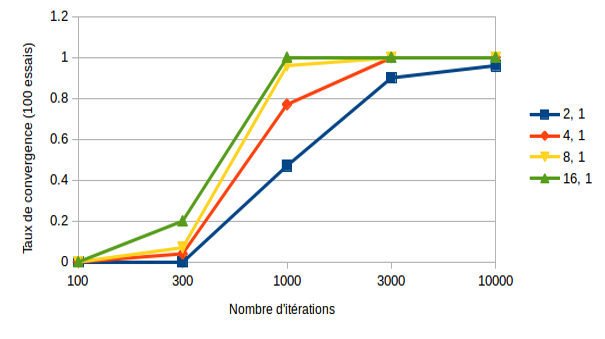
\includegraphics[scale=0.6]{images/xor_architecture_tanh.png}
\caption{Convergence en fonction de l'architecture avec tanh}
\label{xor_architecture_tanh}
\end{center}
\end{figure}

\begin{figure}[!h]
\begin{center}
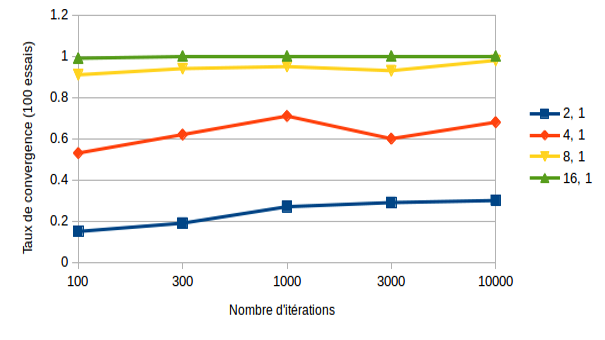
\includegraphics[scale=0.6]{images/xor_architecture_relu.png}
\caption{Convergence en fonction de l'architecture avec relu}
\label{xor_architecture_relu}
\end{center}
\end{figure}

L'exemple de ces deux situations représente clairement les problèmes rencontrés pour étudier les influences des paramètres d'un réseau de neurone. En effet, l'influence de la taille de la couche cachée sur notre réseau n'est plus du tout la même selon le choix de la fonction d'activation appliquée à chaque neurone. Ainsi, il n'est souvent pas possible de définir une règle générale à appliquer concernant un paramètre pris indépendamment des autres.

\section{\'Etude de MNIST}

\subsection{Introduction}
Dans cette partie, mis à part les paramètres explicitement précisés pour un exemple, toutes les mesures qui vont être présentées furent réalisées en utilisant les paramètres suivants :
\begin{itemize}
\item Pas de couche cachée, les neurones d'entrée sont directement reliés aux sorties
\item Les entrées sont centrées et normalisées : chaque pixel est alors représenté par une valeur de [-1;1]
\item Les poids sont initialisés aléatoirement avec une fonction Gaussienne centrée de variance 0,1
\item On utilise une sigmoïde en sortie
\item On utilise l'erreur quadratique pour la fonction de coût
\item Les exemples sont traités pas batch de 128
\item On fixe un learning rate de 0,1
\end{itemize}

\subsection{Architecture du réseau}

Le nombre de couches cachées d'un réseau de neurones ainsi que leur composition constitue l'architecture de ce réseau.

De façon intuitive, il parait évident qu'une plus grande architecture de réseau, possédant plus de neurones par couches cachées ou plus de couches cachées apprendra avec plus de précision l'ensemble de données. Cependant cela a un coût en temps et rendra l'apprentissage beaucoup plus lent.
Ainsi, alors qu'un apprentissage effectué sans couche cachée sur 30 passages du set de données mnist aura une précision d'environ 93\%, un réseau composé d'une couche cachée de 400 neurones ayant pour fonction d'activation tangente hyperbolique pourra avoir sur ce même ensemble presque 98\% de précision. Le résultat de cette seconde situation est visible en figure \ref{mnist100}. On y remarque que l'ensemble de données est très rapidement complètement appris.
\begin{figure}[!h]
\begin{center}
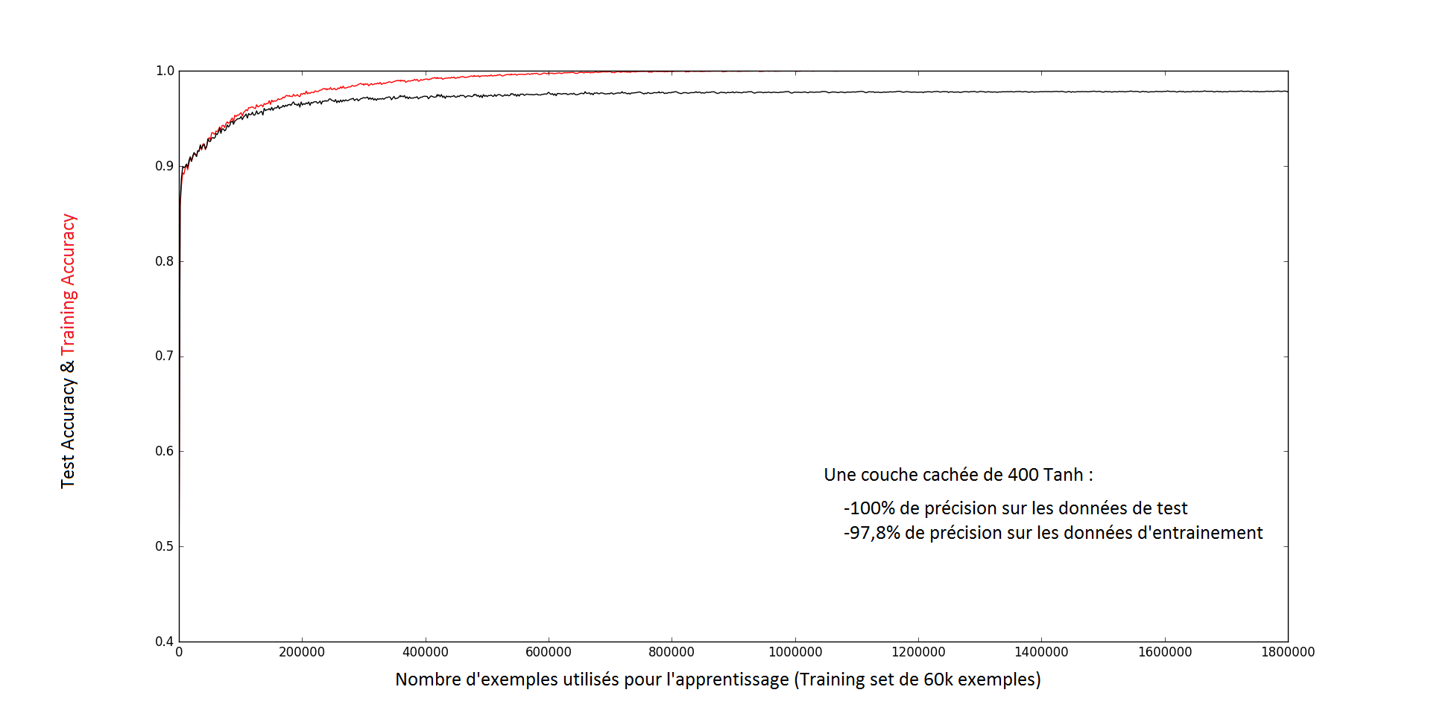
\includegraphics[scale=0.5]{images/mnist100.png}
\caption{Précision pour un réseau avec une couche cachée de 400 neurones}
\label{mnist100}
\end{center}
\end{figure}

\subsection{Initialisation des poids}
Avant le lancement de l'algorithme sur un réseau de neurone, il est nécessaire d'initialiser les poids. L'usage le plus courant est de les initialiser aléatoirement. Cependant, le choix de la distribution aléatoire n'est pas forcément évident. En effet, on peut choisir d'utiliser une distribution uniforme, une distribution gaussienne ou tout autre type de distribution aléatoire avec des paramètres variables.

Nous avons donc testé trois types de fonction d'initialisation des poids : une répartition uniforme, une répartition uniforme centrée en 0  et une répartition gaussienne centrée en 0.
Si les initialisations centrées en 0 permettent une convergence un petit peu plus rapide, ces trois initialisations produisent des résultats similaires. Cependant, l'amplitude des poids change beaucoup les résultats quelle que soit la fonction d'initialisation. En effet, les poids convergeant lors de l'apprentissage vers de petites valeurs, une initialisation avec de petites amplitudes va permettre une convergence plus rapide.

\begin{figure}[!h]
\begin{center}
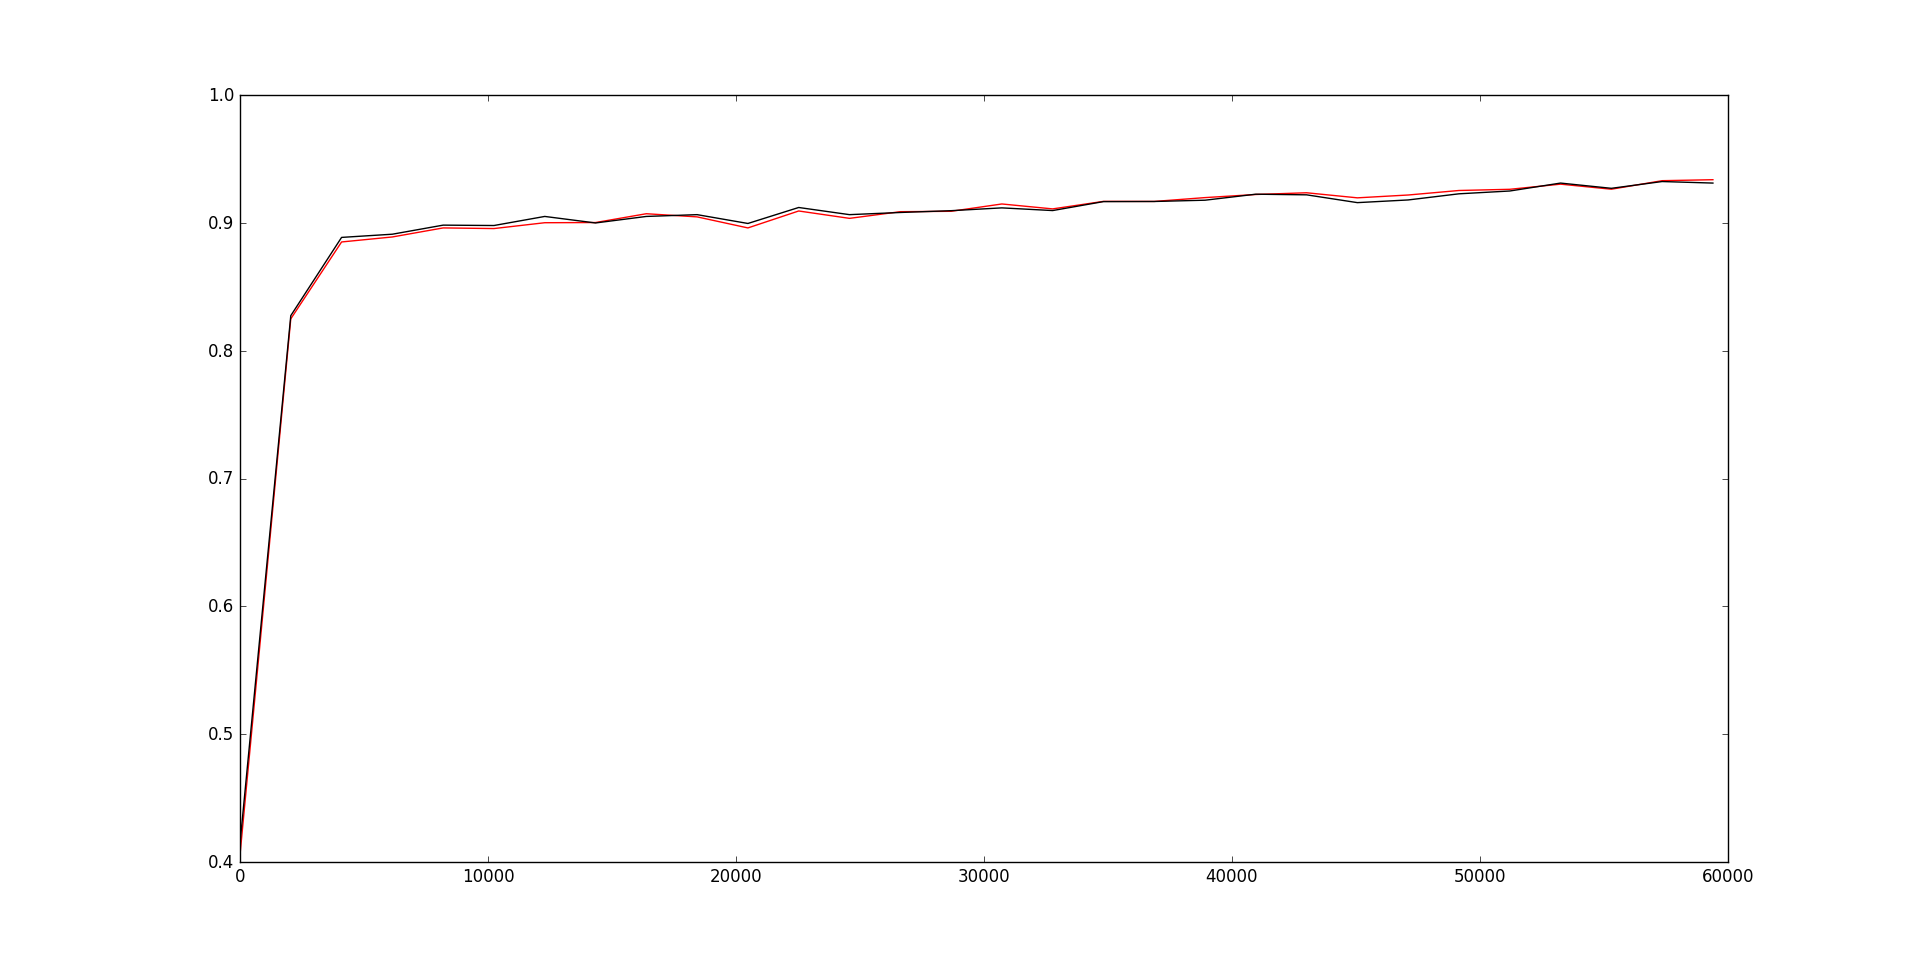
\includegraphics[scale=0.2]{images/initialisationpoids_amplitude01.png}
\caption{Précision sur les ensembles de test (en noir) et d'apprentissage (en rouge) en fonction du nombre d'exemples utilisés pour l'apprentissage pour une initialisation des poids d'amplitude 0.1 }
\label{initialisationpoids_amplitude0.1}
\end{center}
\end{figure}

\begin{figure}[!h]
\begin{center}
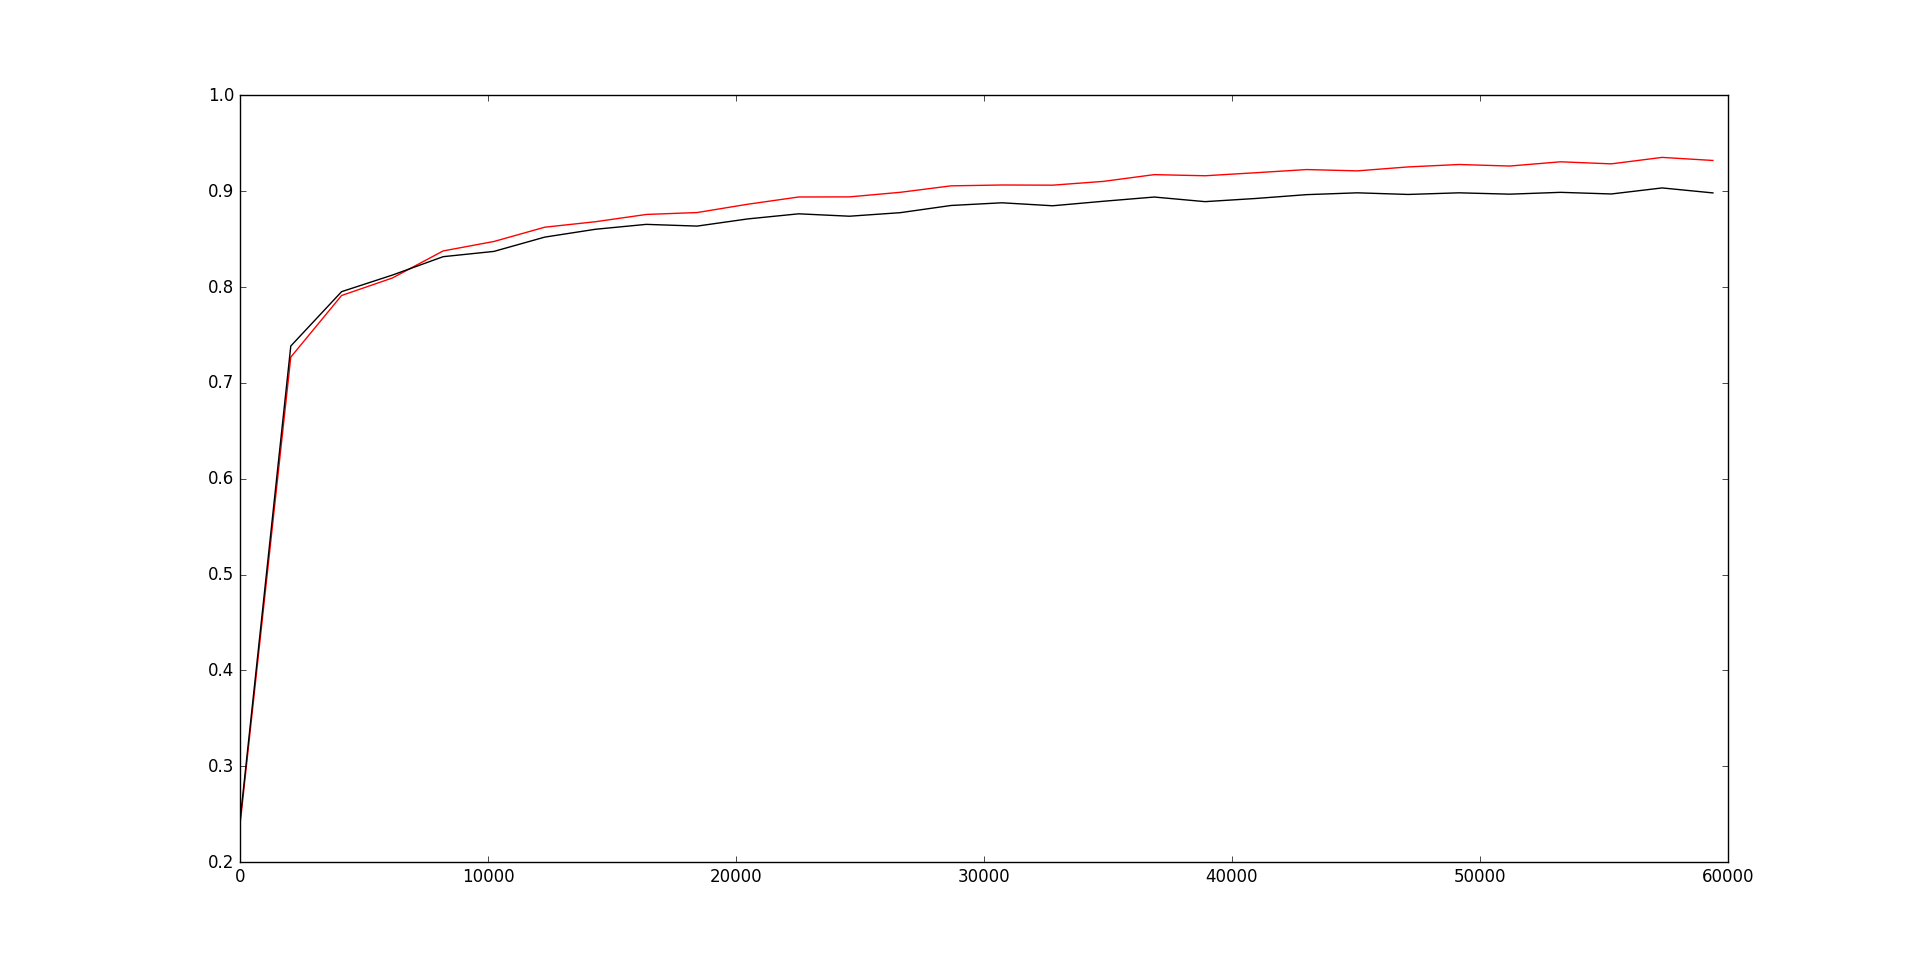
\includegraphics[scale=0.2]{images/initialisationpoids_amplitude10.png}
\caption{Précision sur les ensembles de test (en noir) et d'apprentissage (en rouge) en fonction du nombre d'exemples utilisés pour l'apprentissage pour une initialisation des poids d'amplitude 0.1}
\label{initialisationpoids_amplitude10}
\end{center}
\end{figure}

C'est ce que l'on peut voir sur les deux figures \ref{initialisationpoids_amplitude0.1} et \ref{initialisationpoids_amplitude10}. Dans les deux cas, les poids sont initialisés selon une loi normale centrée de variance 0,1. Cependant, sur la première, un coefficient multiplicatif de 0,1 leur est affecté alors que celui-ci est de 10 sur la deuxième.
On peut ainsi bien observer que dans le cas du facteur multiplicatif de 10, la convergence est plus lente au début de l'apprentissage, même si l'on atteint sensiblement les mêmes valeurs finales de précision.



\subsection{Choix des fonctions d'activations et de coût}

Le tableau \ref{influence_fonction_cout} présente quelques résultats sur la précision obtenu par le réseau selon les fonctions de coût et les fonctions en sortie utilisées.
\begin{figure}[!h]
\begin{center}
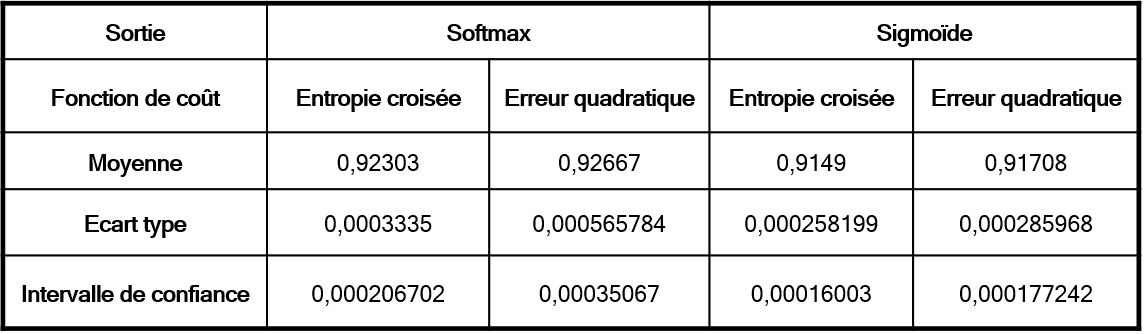
\includegraphics[scale=0.6]{images/influence_fonction_cout.png}
\caption{Influence de la fonction de coût sur la précision obtenue par le réseau}
\label{influence_fonction_cout}
\end{center}
\end{figure}
Le choix de la fonction de coût ne semble avoir qu'un impact très mineur sur les résultats obtenus par le réseau. L'erreur quadratique présente des performances légèrement supérieures à l'entropie croisée pour ce problème mais cette différence est très faible.

En revanche il apparait que l'utilisation de la fonction Softmax en sortie donne de meilleurs résultats que celle d'une sigmoïde. L'emploi de Softmax entrainant un cout en temps plus important que celui de Sigmoïde, cet avantage est à relativiser.


\subsection{Taille des batchs et nombre de passages}

La taille d'un batch est le nombre d'exemples que l'on insère dans le réseau entre chaque rétropropagation du gradient.

\begin{figure}[!h]
\begin{center}
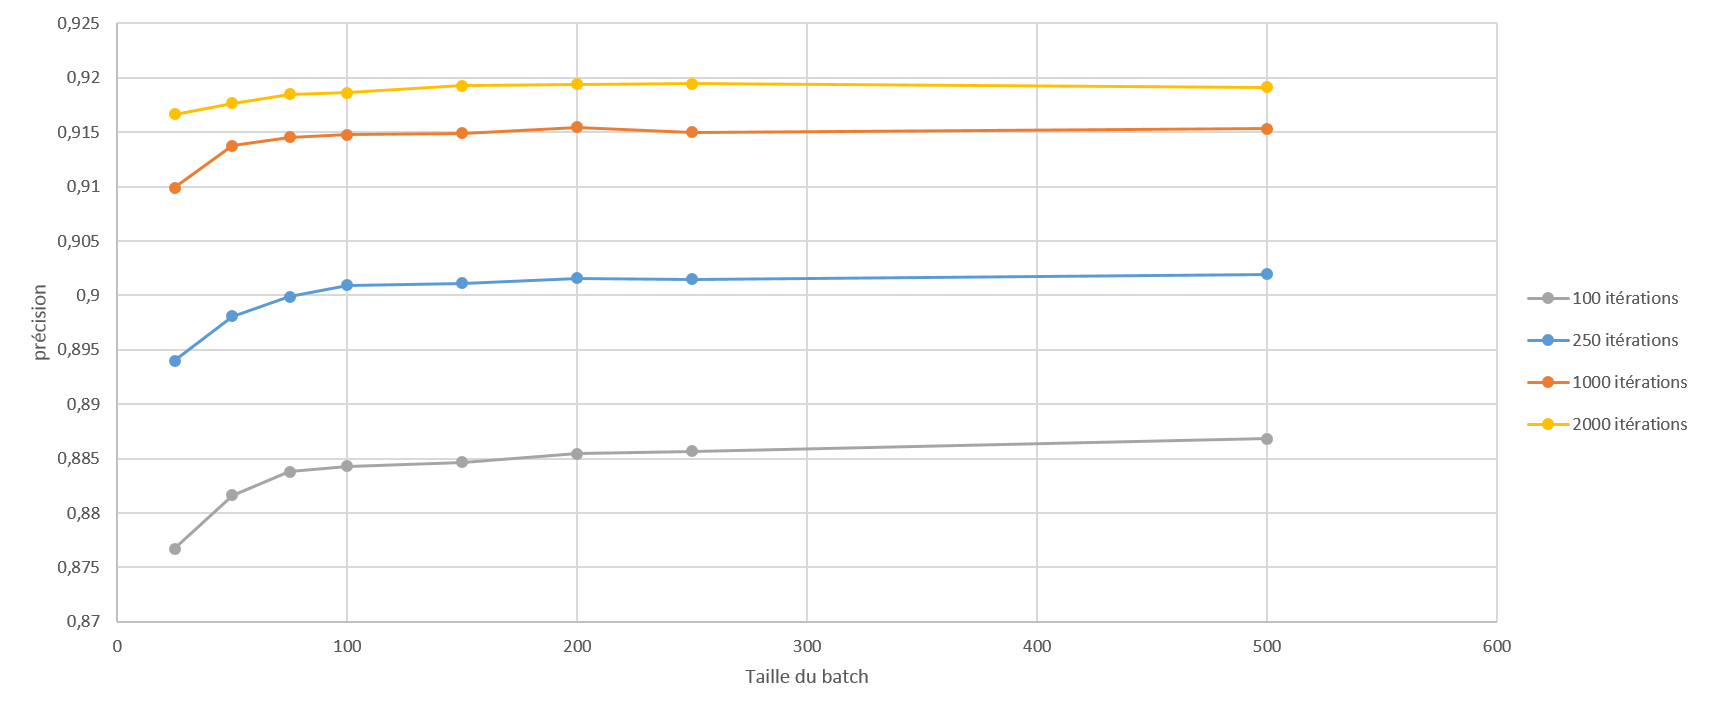
\includegraphics[scale=0.5]{images/precision_taille_batch.png}
\caption{Influence de la taille du batch}
\label{precision_taille_batch}
\end{center}
\end{figure}

La figure \ref{precision_taille_batch} présente la précision obtenue pour différentes tailles de batch. On remarque qu'au delà de 150,augmenter la taille du batch n'améliore presque plus les performances du réseau.
La figure \ref{precision_batch_temps} présente les mêmes données que la figure \ref{precision_taille_batch} mais répartis en fonction du temps de calcul. Utiliser des batchs plus petits semble être plus efficace pour l'apprentissage des données mnist.

\begin{figure}[!h]
\begin{center}
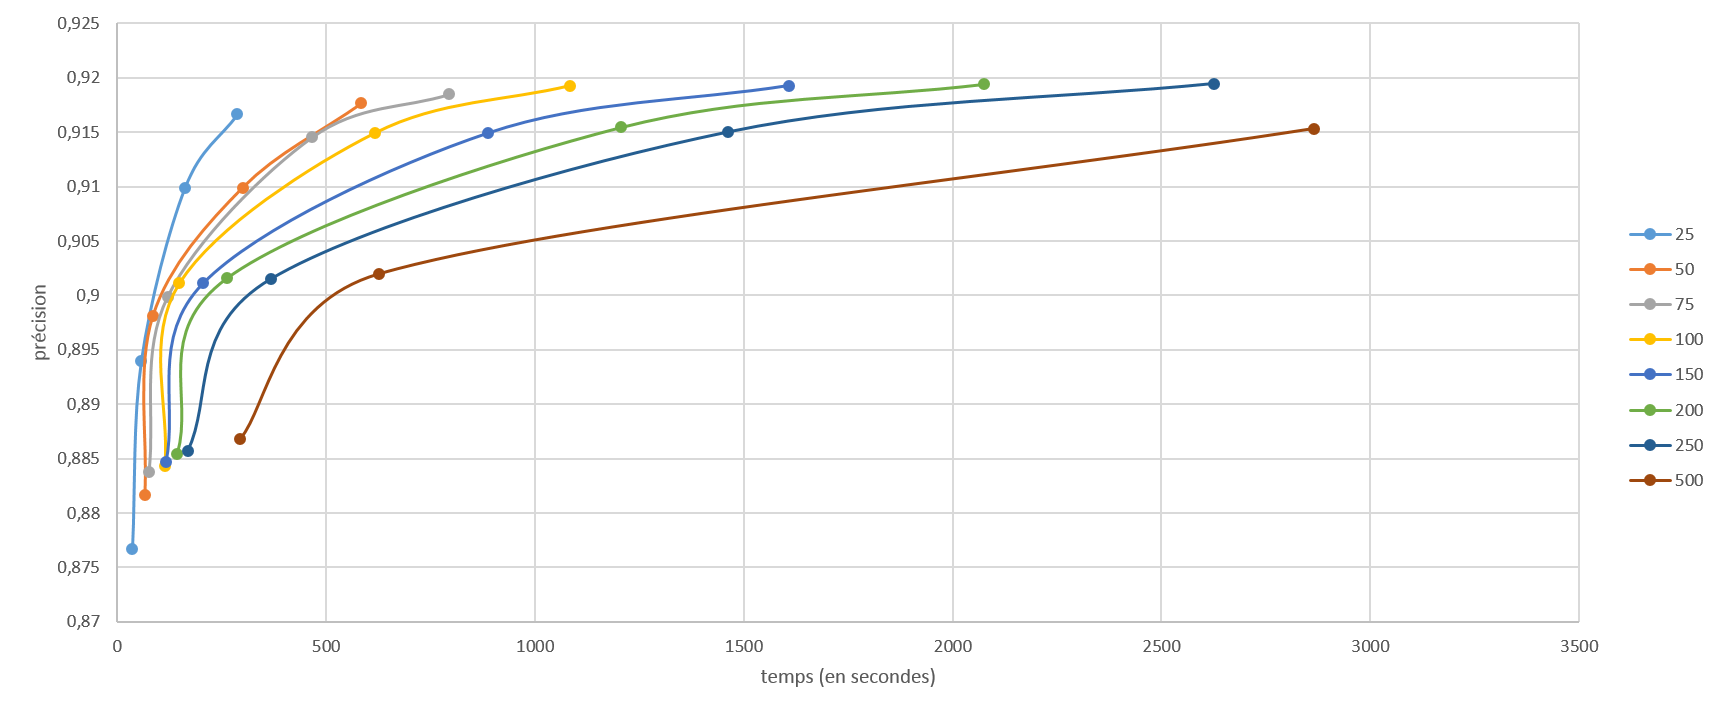
\includegraphics[scale=0.5]{images/precision_batch_temps.png}
\caption{Influence de la taille du batch sur le temps de calcul}
\label{precision_batch_temps}
\end{center}
\end{figure}


\subsection{Taux d'apprentissage}
Nous avons aussi étudié l'influence du taux d'apprentissage ou learning rate. En effet celui-ci influe sur la mise à jour des poids : plus il est grand et plus chaque l'importance donnée au calcul de la dérivée est important. Avoir un taux d'apprentissage grand permet d’obtenir rapidement des performances satisfaisantes en termes de précision. Au contraire, des phénomènes d'oscillations sont observés pour un apprentissage conséquent, et cela fournit en retour de moins bons résultats, par rapport à des taux d'apprentissage plus faibles. Cela a été illustré sur la figure \ref{influence_learningrate}.

\begin{figure}[!h]
\begin{center}
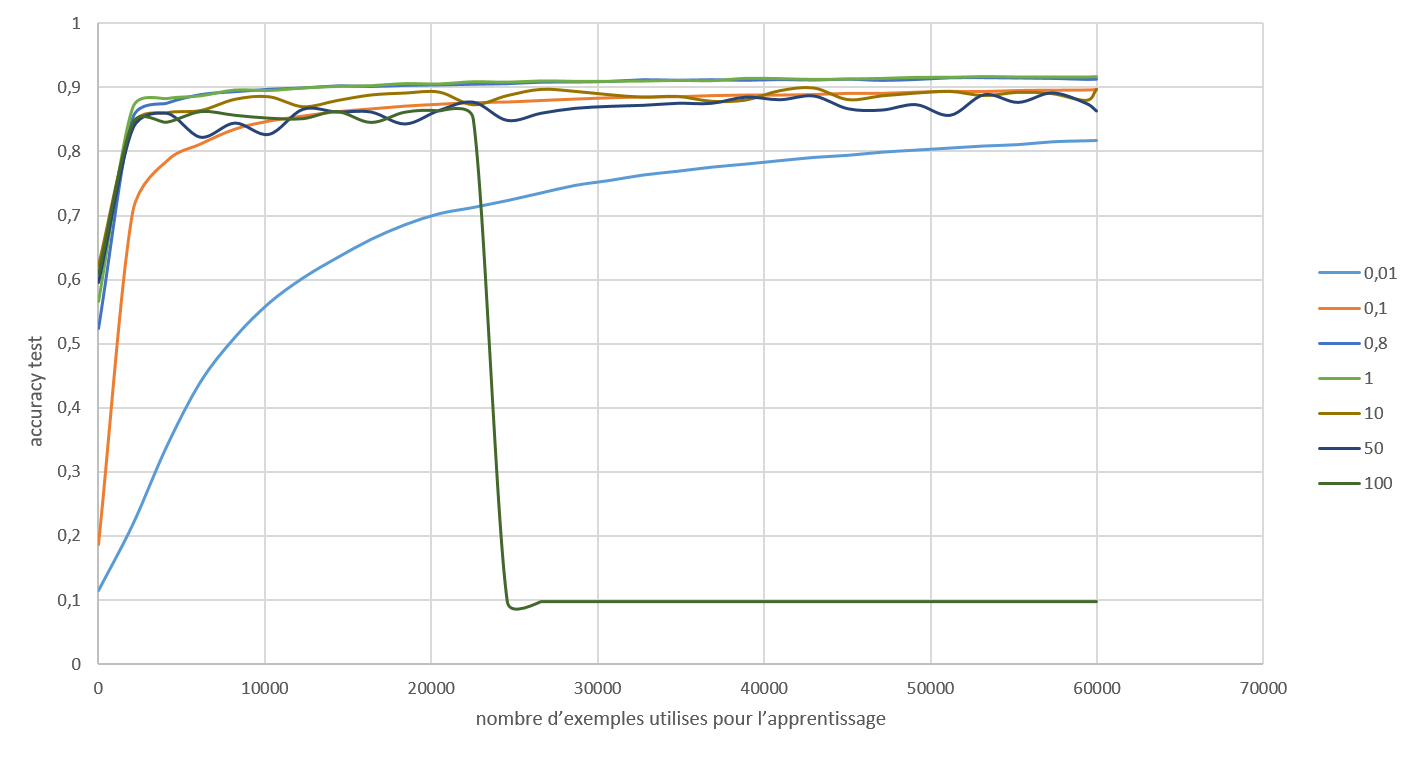
\includegraphics[scale=0.6]{images/influence_learningrate.png}
\caption{Influence du learning rate sur la précision sur l'ensemble de test en fonction du nombre d'exemple utilisés}
\label{influence_learningrate}
\end{center}
\end{figure}

Nous avons alors étudié l'apprentissage du réseau pour des taux d'apprentissage allant de 0.01 à 100.
Nous pouvons alors distinguer trois cas reflétant les principaux comportements :

\begin{itemize}
\item Pour un taux d'apprentissage de 0.01, la convergence est très lente mais sans oscillations. Si la précision obtenue peut-être à hauteur des autres taux d'apprentissage en utilisant plus d'exemples, on peut considérer celui-ci trop petit.
\item Pour un taux d'apprentissage de 100, la convergence est très rapide au début, mais oscille beaucoup et va finalement bloquer l'apprentissage vers un autre minimum local de coût non désiré. On peut donc considérer ce taux d'apprentissage comme trop grand.
\item Pour un taux d'apprentissage de 0.1, il semble apparaître un bon compromis entre stabilité et vitesse de la convergence. C'est cette valeur qui en général sera choisie pour les tests, bien que d'autres soient satisfaisants (0.8 ou 1 par exemple).
\end{itemize}

\chapter{Réseaux de neurones récurrents}

\section{Motivation}

Nous avons pu voir que les réseaux feedforward peuvent être utilisés afin d'appendre à prédire la sortie voulue en fonction de l'entrée du réseau. 

Néanmoins, ces réseaux sont limités à des entrées et des sorties de tailles fixes. De plus il ne peuvent gérer des réseaux présentant des cycles. On utilise alors des réseaux récurrents qui permettent un traitement plus efficace des séquences de données. On pourra ainsi faire de la prédiction et de la génération de séquence.

Dans un premier, nous verrons comment modéliser ces réseaux récurrents. Puis nous nous intéresserons à deux algorithmes d'optimisation permettant l'apprentissage des réseaux récurrents : real time recurrent learning (RTRL) et backpropagation through time (BPTT).

\section{Dépliage}

Nous avons dit précédemment qu'un réseau de neurones récurrent est un réseau possédant des cycles. Néanmoins, il est difficile d'imaginer que la valeur de sortie d'un neurone au temps $t$ dépende de la sortie de ce même neurone au temps $t$. Pour résoudre ce problème, nous allons ajouter une dimension temporelle à nos réseaux et permettre aux neurones au temps $t$ de dépendre des valeurs d'autres neurones au temps $t-1$.

Afin de mettre en évidence cette dépendance temporelle sur nos graphes, les arêtes reliant la sortie d'un neurone au temps $t-1$ à un neurone au temps $t$ vont être annotées par un carré comme sur la figure \ref{arete_retard}. On les appelera arête "retard".

\begin{figure}
\begin{center}
% Graphic for TeX using PGF
% Title: /home/pierre/Programming/pl-lstm/images/illustrations_cr/recurrent_edge.dia
% Creator: Dia v0.97.3
% CreationDate: Sun Jun 11 14:25:19 2017
% For: pierre
% \usepackage{tikz}
% The following commands are not supported in PSTricks at present
% We define them conditionally, so when they are implemented,
% this pgf file will use them.
\ifx\du\undefined
  \newlength{\du}
\fi
\setlength{\du}{15\unitlength}
\begin{tikzpicture}
\pgftransformxscale{1.000000}
\pgftransformyscale{-1.000000}
\definecolor{dialinecolor}{rgb}{0.000000, 0.000000, 0.000000}
\pgfsetstrokecolor{dialinecolor}
\definecolor{dialinecolor}{rgb}{1.000000, 1.000000, 1.000000}
\pgfsetfillcolor{dialinecolor}
\definecolor{dialinecolor}{rgb}{1.000000, 1.000000, 1.000000}
\pgfsetfillcolor{dialinecolor}
\pgfpathellipse{\pgfpoint{20.500000\du}{11.500000\du}}{\pgfpoint{1.500000\du}{0\du}}{\pgfpoint{0\du}{1.500000\du}}
\pgfusepath{fill}
\pgfsetlinewidth{0.100000\du}
\pgfsetdash{}{0pt}
\pgfsetdash{}{0pt}
\definecolor{dialinecolor}{rgb}{0.000000, 0.000000, 0.000000}
\pgfsetstrokecolor{dialinecolor}
\pgfpathellipse{\pgfpoint{20.500000\du}{11.500000\du}}{\pgfpoint{1.500000\du}{0\du}}{\pgfpoint{0\du}{1.500000\du}}
\pgfusepath{stroke}
\pgfsetlinewidth{0.100000\du}
\pgfsetdash{}{0pt}
\pgfsetdash{}{0pt}
\pgfsetmiterjoin
\pgfsetbuttcap
{
\definecolor{dialinecolor}{rgb}{0.000000, 0.000000, 0.000000}
\pgfsetfillcolor{dialinecolor}
% was here!!!
\pgfsetarrowsend{latex}
\definecolor{dialinecolor}{rgb}{0.000000, 0.000000, 0.000000}
\pgfsetstrokecolor{dialinecolor}
\pgfpathmoveto{\pgfpoint{21.560660\du}{10.439340\du}}
\pgfpathcurveto{\pgfpoint{24.000000\du}{9.500000\du}}{\pgfpoint{24.000000\du}{13.500000\du}}{\pgfpoint{21.560660\du}{12.560660\du}}
\pgfusepath{stroke}
}
\definecolor{dialinecolor}{rgb}{1.000000, 1.000000, 1.000000}
\pgfsetfillcolor{dialinecolor}
\pgfpathellipse{\pgfpoint{20.500000\du}{16.500000\du}}{\pgfpoint{1.500000\du}{0\du}}{\pgfpoint{0\du}{1.500000\du}}
\pgfusepath{fill}
\pgfsetlinewidth{0.100000\du}
\pgfsetdash{}{0pt}
\pgfsetdash{}{0pt}
\definecolor{dialinecolor}{rgb}{0.000000, 0.000000, 0.000000}
\pgfsetstrokecolor{dialinecolor}
\pgfpathellipse{\pgfpoint{20.500000\du}{16.500000\du}}{\pgfpoint{1.500000\du}{0\du}}{\pgfpoint{0\du}{1.500000\du}}
\pgfusepath{stroke}
\pgfsetlinewidth{0.100000\du}
\pgfsetdash{}{0pt}
\pgfsetdash{}{0pt}
\pgfsetbuttcap
{
\definecolor{dialinecolor}{rgb}{0.000000, 0.000000, 0.000000}
\pgfsetfillcolor{dialinecolor}
% was here!!!
\pgfsetarrowsend{latex}
\definecolor{dialinecolor}{rgb}{0.000000, 0.000000, 0.000000}
\pgfsetstrokecolor{dialinecolor}
\draw (20.500000\du,15.000000\du)--(20.500000\du,13.000000\du);
}
\pgfsetlinewidth{0.100000\du}
\pgfsetdash{}{0pt}
\pgfsetdash{}{0pt}
\pgfsetmiterjoin
\definecolor{dialinecolor}{rgb}{0.000000, 0.000000, 0.000000}
\pgfsetfillcolor{dialinecolor}
\fill (23.200000\du,11.200000\du)--(23.200000\du,11.700000\du)--(23.700000\du,11.700000\du)--(23.700000\du,11.200000\du)--cycle;
\definecolor{dialinecolor}{rgb}{0.000000, 0.000000, 0.000000}
\pgfsetstrokecolor{dialinecolor}
\draw (23.200000\du,11.200000\du)--(23.200000\du,11.700000\du)--(23.700000\du,11.700000\du)--(23.700000\du,11.200000\du)--cycle;
% setfont left to latex
\definecolor{dialinecolor}{rgb}{0.000000, 0.000000, 0.000000}
\pgfsetstrokecolor{dialinecolor}
\node at (20.500000\du,11.722500\du){$h$};
% setfont left to latex
\definecolor{dialinecolor}{rgb}{0.000000, 0.000000, 0.000000}
\pgfsetstrokecolor{dialinecolor}
\node at (20.500000\du,16.722500\du){$x$};
\end{tikzpicture}

\caption{Réseau de neurones récurrent où l'arête avec un carré signifie que le n\oe{}ud $h$ prend sa valeur au temps $t-1$ comme entrée au temps $t$.}
\label{arete_retard}
\end{center}
\end{figure}

On peut maintenant remarquer que pour une séquence $x_1, ..., x_n$ le réseau récurrent de la figure \ref{arete_retard} est équivalent au réseau feedforward de la figure \ref{reseau_deplie}.

\begin{figure}
\begin{center}
% Graphic for TeX using PGF
% Title: /home/pierre/Programming/pl-lstm/images/illustrations_cr/unfolded_graph.dia
% Creator: Dia v0.97.3
% CreationDate: Sun Jun 11 14:43:00 2017
% For: pierre
% \usepackage{tikz}
% The following commands are not supported in PSTricks at present
% We define them conditionally, so when they are implemented,
% this pgf file will use them.
\ifx\du\undefined
  \newlength{\du}
\fi
\setlength{\du}{15\unitlength}
\begin{tikzpicture}
\pgftransformxscale{1.000000}
\pgftransformyscale{-1.000000}
\definecolor{dialinecolor}{rgb}{0.000000, 0.000000, 0.000000}
\pgfsetstrokecolor{dialinecolor}
\definecolor{dialinecolor}{rgb}{1.000000, 1.000000, 1.000000}
\pgfsetfillcolor{dialinecolor}
\definecolor{dialinecolor}{rgb}{1.000000, 1.000000, 1.000000}
\pgfsetfillcolor{dialinecolor}
\pgfpathellipse{\pgfpoint{20.500000\du}{11.500000\du}}{\pgfpoint{1.500000\du}{0\du}}{\pgfpoint{0\du}{1.500000\du}}
\pgfusepath{fill}
\pgfsetlinewidth{0.100000\du}
\pgfsetdash{}{0pt}
\pgfsetdash{}{0pt}
\definecolor{dialinecolor}{rgb}{0.000000, 0.000000, 0.000000}
\pgfsetstrokecolor{dialinecolor}
\pgfpathellipse{\pgfpoint{20.500000\du}{11.500000\du}}{\pgfpoint{1.500000\du}{0\du}}{\pgfpoint{0\du}{1.500000\du}}
\pgfusepath{stroke}
\definecolor{dialinecolor}{rgb}{1.000000, 1.000000, 1.000000}
\pgfsetfillcolor{dialinecolor}
\pgfpathellipse{\pgfpoint{20.500000\du}{16.500000\du}}{\pgfpoint{1.500000\du}{0\du}}{\pgfpoint{0\du}{1.500000\du}}
\pgfusepath{fill}
\pgfsetlinewidth{0.100000\du}
\pgfsetdash{}{0pt}
\pgfsetdash{}{0pt}
\definecolor{dialinecolor}{rgb}{0.000000, 0.000000, 0.000000}
\pgfsetstrokecolor{dialinecolor}
\pgfpathellipse{\pgfpoint{20.500000\du}{16.500000\du}}{\pgfpoint{1.500000\du}{0\du}}{\pgfpoint{0\du}{1.500000\du}}
\pgfusepath{stroke}
\pgfsetlinewidth{0.100000\du}
\pgfsetdash{}{0pt}
\pgfsetdash{}{0pt}
\pgfsetbuttcap
{
\definecolor{dialinecolor}{rgb}{0.000000, 0.000000, 0.000000}
\pgfsetfillcolor{dialinecolor}
% was here!!!
\pgfsetarrowsend{latex}
\definecolor{dialinecolor}{rgb}{0.000000, 0.000000, 0.000000}
\pgfsetstrokecolor{dialinecolor}
\draw (20.500000\du,15.000000\du)--(20.500000\du,13.000000\du);
}
% setfont left to latex
\definecolor{dialinecolor}{rgb}{0.000000, 0.000000, 0.000000}
\pgfsetstrokecolor{dialinecolor}
\node at (20.500000\du,11.722500\du){$h(1)$};
% setfont left to latex
\definecolor{dialinecolor}{rgb}{0.000000, 0.000000, 0.000000}
\pgfsetstrokecolor{dialinecolor}
\node at (20.500000\du,16.722500\du){$x_1$};
\definecolor{dialinecolor}{rgb}{1.000000, 1.000000, 1.000000}
\pgfsetfillcolor{dialinecolor}
\pgfpathellipse{\pgfpoint{25.500000\du}{11.500000\du}}{\pgfpoint{1.500000\du}{0\du}}{\pgfpoint{0\du}{1.500000\du}}
\pgfusepath{fill}
\pgfsetlinewidth{0.100000\du}
\pgfsetdash{}{0pt}
\pgfsetdash{}{0pt}
\definecolor{dialinecolor}{rgb}{0.000000, 0.000000, 0.000000}
\pgfsetstrokecolor{dialinecolor}
\pgfpathellipse{\pgfpoint{25.500000\du}{11.500000\du}}{\pgfpoint{1.500000\du}{0\du}}{\pgfpoint{0\du}{1.500000\du}}
\pgfusepath{stroke}
\definecolor{dialinecolor}{rgb}{1.000000, 1.000000, 1.000000}
\pgfsetfillcolor{dialinecolor}
\pgfpathellipse{\pgfpoint{25.500000\du}{16.500000\du}}{\pgfpoint{1.500000\du}{0\du}}{\pgfpoint{0\du}{1.500000\du}}
\pgfusepath{fill}
\pgfsetlinewidth{0.100000\du}
\pgfsetdash{}{0pt}
\pgfsetdash{}{0pt}
\definecolor{dialinecolor}{rgb}{0.000000, 0.000000, 0.000000}
\pgfsetstrokecolor{dialinecolor}
\pgfpathellipse{\pgfpoint{25.500000\du}{16.500000\du}}{\pgfpoint{1.500000\du}{0\du}}{\pgfpoint{0\du}{1.500000\du}}
\pgfusepath{stroke}
\pgfsetlinewidth{0.100000\du}
\pgfsetdash{}{0pt}
\pgfsetdash{}{0pt}
\pgfsetbuttcap
{
\definecolor{dialinecolor}{rgb}{0.000000, 0.000000, 0.000000}
\pgfsetfillcolor{dialinecolor}
% was here!!!
\pgfsetarrowsend{latex}
\definecolor{dialinecolor}{rgb}{0.000000, 0.000000, 0.000000}
\pgfsetstrokecolor{dialinecolor}
\draw (25.500000\du,15.000000\du)--(25.500000\du,13.000000\du);
}
\definecolor{dialinecolor}{rgb}{1.000000, 1.000000, 1.000000}
\pgfsetfillcolor{dialinecolor}
\pgfpathellipse{\pgfpoint{34.500000\du}{11.500000\du}}{\pgfpoint{1.500000\du}{0\du}}{\pgfpoint{0\du}{1.500000\du}}
\pgfusepath{fill}
\pgfsetlinewidth{0.100000\du}
\pgfsetdash{}{0pt}
\pgfsetdash{}{0pt}
\definecolor{dialinecolor}{rgb}{0.000000, 0.000000, 0.000000}
\pgfsetstrokecolor{dialinecolor}
\pgfpathellipse{\pgfpoint{34.500000\du}{11.500000\du}}{\pgfpoint{1.500000\du}{0\du}}{\pgfpoint{0\du}{1.500000\du}}
\pgfusepath{stroke}
\definecolor{dialinecolor}{rgb}{1.000000, 1.000000, 1.000000}
\pgfsetfillcolor{dialinecolor}
\pgfpathellipse{\pgfpoint{34.500000\du}{16.500000\du}}{\pgfpoint{1.500000\du}{0\du}}{\pgfpoint{0\du}{1.500000\du}}
\pgfusepath{fill}
\pgfsetlinewidth{0.100000\du}
\pgfsetdash{}{0pt}
\pgfsetdash{}{0pt}
\definecolor{dialinecolor}{rgb}{0.000000, 0.000000, 0.000000}
\pgfsetstrokecolor{dialinecolor}
\pgfpathellipse{\pgfpoint{34.500000\du}{16.500000\du}}{\pgfpoint{1.500000\du}{0\du}}{\pgfpoint{0\du}{1.500000\du}}
\pgfusepath{stroke}
\pgfsetlinewidth{0.100000\du}
\pgfsetdash{}{0pt}
\pgfsetdash{}{0pt}
\pgfsetbuttcap
{
\definecolor{dialinecolor}{rgb}{0.000000, 0.000000, 0.000000}
\pgfsetfillcolor{dialinecolor}
% was here!!!
\pgfsetarrowsend{latex}
\definecolor{dialinecolor}{rgb}{0.000000, 0.000000, 0.000000}
\pgfsetstrokecolor{dialinecolor}
\draw (34.500000\du,15.000000\du)--(34.500000\du,13.000000\du);
}
\pgfsetlinewidth{0.100000\du}
\pgfsetdash{}{0pt}
\pgfsetdash{}{0pt}
\pgfsetbuttcap
{
\definecolor{dialinecolor}{rgb}{0.000000, 0.000000, 0.000000}
\pgfsetfillcolor{dialinecolor}
% was here!!!
\pgfsetarrowsend{latex}
\definecolor{dialinecolor}{rgb}{0.000000, 0.000000, 0.000000}
\pgfsetstrokecolor{dialinecolor}
\draw (22.000000\du,11.500000\du)--(23.950806\du,11.500000\du);
}
\definecolor{dialinecolor}{rgb}{1.000000, 1.000000, 1.000000}
\pgfsetfillcolor{dialinecolor}
\pgfpathellipse{\pgfpoint{39.500000\du}{11.500000\du}}{\pgfpoint{1.500000\du}{0\du}}{\pgfpoint{0\du}{1.500000\du}}
\pgfusepath{fill}
\pgfsetlinewidth{0.100000\du}
\pgfsetdash{}{0pt}
\pgfsetdash{}{0pt}
\definecolor{dialinecolor}{rgb}{0.000000, 0.000000, 0.000000}
\pgfsetstrokecolor{dialinecolor}
\pgfpathellipse{\pgfpoint{39.500000\du}{11.500000\du}}{\pgfpoint{1.500000\du}{0\du}}{\pgfpoint{0\du}{1.500000\du}}
\pgfusepath{stroke}
\definecolor{dialinecolor}{rgb}{1.000000, 1.000000, 1.000000}
\pgfsetfillcolor{dialinecolor}
\pgfpathellipse{\pgfpoint{39.500000\du}{16.500000\du}}{\pgfpoint{1.500000\du}{0\du}}{\pgfpoint{0\du}{1.500000\du}}
\pgfusepath{fill}
\pgfsetlinewidth{0.100000\du}
\pgfsetdash{}{0pt}
\pgfsetdash{}{0pt}
\definecolor{dialinecolor}{rgb}{0.000000, 0.000000, 0.000000}
\pgfsetstrokecolor{dialinecolor}
\pgfpathellipse{\pgfpoint{39.500000\du}{16.500000\du}}{\pgfpoint{1.500000\du}{0\du}}{\pgfpoint{0\du}{1.500000\du}}
\pgfusepath{stroke}
\pgfsetlinewidth{0.100000\du}
\pgfsetdash{}{0pt}
\pgfsetdash{}{0pt}
\pgfsetbuttcap
{
\definecolor{dialinecolor}{rgb}{0.000000, 0.000000, 0.000000}
\pgfsetfillcolor{dialinecolor}
% was here!!!
\pgfsetarrowsend{latex}
\definecolor{dialinecolor}{rgb}{0.000000, 0.000000, 0.000000}
\pgfsetstrokecolor{dialinecolor}
\draw (39.500000\du,15.000000\du)--(39.500000\du,13.000000\du);
}
\pgfsetlinewidth{0.100000\du}
\pgfsetdash{}{0pt}
\pgfsetdash{}{0pt}
\pgfsetbuttcap
{
\definecolor{dialinecolor}{rgb}{0.000000, 0.000000, 0.000000}
\pgfsetfillcolor{dialinecolor}
% was here!!!
\pgfsetarrowsend{latex}
\definecolor{dialinecolor}{rgb}{0.000000, 0.000000, 0.000000}
\pgfsetstrokecolor{dialinecolor}
\draw (36.000000\du,11.500000\du)--(37.950806\du,11.500000\du);
}
% setfont left to latex
\definecolor{dialinecolor}{rgb}{0.000000, 0.000000, 0.000000}
\pgfsetstrokecolor{dialinecolor}
\node at (25.500000\du,16.722500\du){$x_2$};
% setfont left to latex
\definecolor{dialinecolor}{rgb}{0.000000, 0.000000, 0.000000}
\pgfsetstrokecolor{dialinecolor}
\node at (34.500000\du,16.722500\du){$x_{n-1}$};
% setfont left to latex
\definecolor{dialinecolor}{rgb}{0.000000, 0.000000, 0.000000}
\pgfsetstrokecolor{dialinecolor}
\node at (39.500000\du,16.722500\du){$x_n$};
% setfont left to latex
\definecolor{dialinecolor}{rgb}{0.000000, 0.000000, 0.000000}
\pgfsetstrokecolor{dialinecolor}
\node at (25.500000\du,11.722500\du){$h(2)$};
% setfont left to latex
\definecolor{dialinecolor}{rgb}{0.000000, 0.000000, 0.000000}
\pgfsetstrokecolor{dialinecolor}
\node at (34.500000\du,11.722500\du){$h(n-1)$};
% setfont left to latex
\definecolor{dialinecolor}{rgb}{0.000000, 0.000000, 0.000000}
\pgfsetstrokecolor{dialinecolor}
\node at (39.500000\du,11.722500\du){$h(n)$};
\pgfsetlinewidth{0.100000\du}
\pgfsetdash{}{0pt}
\pgfsetdash{}{0pt}
\pgfsetbuttcap
{
\definecolor{dialinecolor}{rgb}{0.000000, 0.000000, 0.000000}
\pgfsetfillcolor{dialinecolor}
% was here!!!
\pgfsetarrowsend{latex}
\definecolor{dialinecolor}{rgb}{0.000000, 0.000000, 0.000000}
\pgfsetstrokecolor{dialinecolor}
\draw (27.000000\du,11.500000\du)--(29.000000\du,11.500000\du);
}
\pgfsetlinewidth{0.100000\du}
\pgfsetdash{}{0pt}
\pgfsetdash{}{0pt}
\pgfsetbuttcap
{
\definecolor{dialinecolor}{rgb}{0.000000, 0.000000, 0.000000}
\pgfsetfillcolor{dialinecolor}
% was here!!!
\pgfsetarrowsend{latex}
\definecolor{dialinecolor}{rgb}{0.000000, 0.000000, 0.000000}
\pgfsetstrokecolor{dialinecolor}
\draw (31.000000\du,11.500000\du)--(33.000000\du,11.500000\du);
}
% setfont left to latex
\definecolor{dialinecolor}{rgb}{0.000000, 0.000000, 0.000000}
\pgfsetstrokecolor{dialinecolor}
\node at (30.000000\du,11.722500\du){$...$};
% setfont left to latex
\definecolor{dialinecolor}{rgb}{0.000000, 0.000000, 0.000000}
\pgfsetstrokecolor{dialinecolor}
\node at (20.500000\du,8.722500\du){$t=1$};
% setfont left to latex
\definecolor{dialinecolor}{rgb}{0.000000, 0.000000, 0.000000}
\pgfsetstrokecolor{dialinecolor}
\node at (25.500000\du,8.722500\du){$t=2$};
% setfont left to latex
\definecolor{dialinecolor}{rgb}{0.000000, 0.000000, 0.000000}
\pgfsetstrokecolor{dialinecolor}
\node at (34.500000\du,8.722500\du){$t=n-1$};
% setfont left to latex
\definecolor{dialinecolor}{rgb}{0.000000, 0.000000, 0.000000}
\pgfsetstrokecolor{dialinecolor}
\node at (39.500000\du,8.722500\du){$t=n$};
\end{tikzpicture}

\caption{Réseau de neurones feedforward équivalent au réseau récurrent de la figure \ref{arete_retard} pour la séquence d'entrée $x_1, ..., x_n$.}
\label{reseau_deplie}
\end{center}
\end{figure}

Le processus de passage d'un réseau récurrent à un réseau feedforward s'appelle dépliage.

Une fois le réseau déplié obtenu, on peut utiliser l'algorithme de propagation classique pour les graphes de calculs afin de calculer la sortie du réseau récurrent.

Nous avons utilisé trois méthodes pour générer des réseaux dépliés. La première prend en entrée un réseau récurrent avec des arêtes retards et obtient le dépliage à partir de celui-ci.

La seconde prend en entrée un \textit{layer}, représenté figure \ref{layer}, c'est-à-dire le sous-graphe qui va être copié à chaque pas de temps et le clone autant de fois qu'il le faut.

\begin{figure}
\begin{center}
% Graphic for TeX using PGF
% Title: /home/pierre/Programming/pl-lstm/images/illustrations_cr/layer.dia
% Creator: Dia v0.97.3
% CreationDate: Wed Mar  8 22:39:59 2017
% For: pierre
% \usepackage{tikz}
% The following commands are not supported in PSTricks at present
% We define them conditionally, so when they are implemented,
% this pgf file will use them.
\ifx\du\undefined
  \newlength{\du}
\fi
\setlength{\du}{15\unitlength}
\begin{tikzpicture}[scale=0.5]
\pgftransformxscale{1.000000}
\pgftransformyscale{-1.000000}
\definecolor{dialinecolor}{rgb}{0.000000, 0.000000, 0.000000}
\pgfsetstrokecolor{dialinecolor}
\definecolor{dialinecolor}{rgb}{1.000000, 1.000000, 1.000000}
\pgfsetfillcolor{dialinecolor}
\pgfsetlinewidth{0.100000\du}
\pgfsetdash{}{0pt}
\pgfsetdash{}{0pt}
\pgfsetmiterjoin
\definecolor{dialinecolor}{rgb}{1.000000, 1.000000, 1.000000}
\pgfsetfillcolor{dialinecolor}
\fill (12.105000\du,6.867500\du)--(12.105000\du,21.867500\du)--(22.105000\du,21.867500\du)--(22.105000\du,6.867500\du)--cycle;
\definecolor{dialinecolor}{rgb}{0.000000, 0.000000, 0.000000}
\pgfsetstrokecolor{dialinecolor}
\draw (12.105000\du,6.867500\du)--(12.105000\du,21.867500\du)--(22.105000\du,21.867500\du)--(22.105000\du,6.867500\du)--cycle;
\pgfsetlinewidth{0.100000\du}
\pgfsetdash{}{0pt}
\pgfsetdash{}{0pt}
\pgfsetbuttcap
{
\definecolor{dialinecolor}{rgb}{0.000000, 0.000000, 0.000000}
\pgfsetfillcolor{dialinecolor}
% was here!!!
\pgfsetarrowsend{latex}
\definecolor{dialinecolor}{rgb}{0.000000, 0.000000, 0.000000}
\pgfsetstrokecolor{dialinecolor}
\draw (17.105000\du,24.867500\du)--(17.105000\du,21.867500\du);
}
\pgfsetlinewidth{0.100000\du}
\pgfsetdash{}{0pt}
\pgfsetdash{}{0pt}
\pgfsetbuttcap
{
\definecolor{dialinecolor}{rgb}{0.000000, 0.000000, 0.000000}
\pgfsetfillcolor{dialinecolor}
% was here!!!
\pgfsetarrowsend{latex}
\definecolor{dialinecolor}{rgb}{0.000000, 0.000000, 0.000000}
\pgfsetstrokecolor{dialinecolor}
\draw (17.105000\du,3.867500\du)--(17.105000\du,6.867500\du);
}
\pgfsetlinewidth{0.100000\du}
\pgfsetdash{}{0pt}
\pgfsetdash{}{0pt}
\pgfsetbuttcap
{
\definecolor{dialinecolor}{rgb}{0.301961, 0.301961, 0.301961}
\pgfsetfillcolor{dialinecolor}
% was here!!!
\pgfsetarrowsend{latex}
\definecolor{dialinecolor}{rgb}{0.301961, 0.301961, 0.301961}
\pgfsetstrokecolor{dialinecolor}
\draw (12.105000\du,13.867500\du)--(8.105000\du,13.867500\du);
}
% setfont left to latex
\definecolor{dialinecolor}{rgb}{0.000000, 0.000000, 0.000000}
\pgfsetstrokecolor{dialinecolor}
\node[anchor=west] at (6.000000\du,13.000000\du){$h_{in}$};
% setfont left to latex
\definecolor{dialinecolor}{rgb}{0.000000, 0.000000, 0.000000}
\pgfsetstrokecolor{dialinecolor}
\node[anchor=west] at (26.305000\du,13.067500\du){$h_{out}$};
% setfont left to latex
\definecolor{dialinecolor}{rgb}{0.301961, 0.301961, 0.301961}
\pgfsetstrokecolor{dialinecolor}
\node[anchor=west] at (5.000000\du,15.000000\du){$\frac{\partial E}{\partial h_{in}}$};
% setfont left to latex
\definecolor{dialinecolor}{rgb}{0.301961, 0.301961, 0.301961}
\pgfsetstrokecolor{dialinecolor}
\node[anchor=west] at (26.305000\du,15.067500\du){$\frac{\partial E}{\partial h_{out}}$};
\pgfsetlinewidth{0.100000\du}
\pgfsetdash{}{0pt}
\pgfsetdash{}{0pt}
\pgfsetbuttcap
{
\definecolor{dialinecolor}{rgb}{0.000000, 0.000000, 0.000000}
\pgfsetfillcolor{dialinecolor}
% was here!!!
\pgfsetarrowsend{latex}
\definecolor{dialinecolor}{rgb}{0.000000, 0.000000, 0.000000}
\pgfsetstrokecolor{dialinecolor}
\draw (8.105000\du,12.867500\du)--(12.105000\du,12.867500\du);
}
\pgfsetlinewidth{0.100000\du}
\pgfsetdash{}{0pt}
\pgfsetdash{}{0pt}
\pgfsetbuttcap
{
\definecolor{dialinecolor}{rgb}{0.301961, 0.301961, 0.301961}
\pgfsetfillcolor{dialinecolor}
% was here!!!
\pgfsetarrowsend{latex}
\definecolor{dialinecolor}{rgb}{0.301961, 0.301961, 0.301961}
\pgfsetstrokecolor{dialinecolor}
\draw (26.105000\du,13.867500\du)--(22.105000\du,13.867500\du);
}
\pgfsetlinewidth{0.100000\du}
\pgfsetdash{}{0pt}
\pgfsetdash{}{0pt}
\pgfsetbuttcap
{
\definecolor{dialinecolor}{rgb}{0.000000, 0.000000, 0.000000}
\pgfsetfillcolor{dialinecolor}
% was here!!!
\pgfsetarrowsend{latex}
\definecolor{dialinecolor}{rgb}{0.000000, 0.000000, 0.000000}
\pgfsetstrokecolor{dialinecolor}
\draw (22.105000\du,12.867500\du)--(26.105000\du,12.867500\du);
}
% setfont left to latex
\definecolor{dialinecolor}{rgb}{0.000000, 0.000000, 0.000000}
\pgfsetstrokecolor{dialinecolor}
\node at (17.105000\du,25.590000\du){$x_t$};
% setfont left to latex
\definecolor{dialinecolor}{rgb}{0.000000, 0.000000, 0.000000}
\pgfsetstrokecolor{dialinecolor}
\node at (17.000000\du,3.222500\du){$y_t$};
\end{tikzpicture}

\caption{Représentation d'un layer. Il contient les n\oe{}uds du graphe à un temps $t$. Il prend en entrée la sortie de l'état caché du temps $t-1$ appelée $h_{in}$ et l'entrée $x_t$. Il a comme sortie l'état caché $h_{out}$ ainsi que $\hat{y}_t$ qui sera comparé avec $y_t$ la sortie attendue au temps $t$. Le $layer$ sert aussi lors de la phase de rétropropagation.}
\label{layer}
\end{center}
\end{figure}

Enfin la dernière méthode est de ne pas utiliser d'algorithme "général" permettant de passer d'un graphe récurrent à un graphe acyclique. Mais plutôt d'écrire pour chaque architecture de réseau une fonction dépliant ce réseau. Une telle fonction contiendra principalement une boucle créant les n\oe{}uds nécessaires pour chaque temps.

Devant la diversité des architectures des réseaux récurrents, la dernière méthode est la plus sensée et la plus pratique. Elle offre une liberté totale quant à l'architecture du graphe tout en étant relativement simple.

\section{BPTT}

Contrairement, à ce que nous avons fait lors du projet, nous allons d'abord présenter l'algorithme \textit{backpropagation through time} (BPTT) car il s'agit d'une simple généralisation de la rétropropagation déjà présentée pour les réseaux feedforward.

L'algorithme consiste en deux étapes :
\begin{enumerate}
\item Déplier le réseau récurrent pour avoir un réseau feedforward.
\item Appliquer l'algorithme de rétropropagation à ce réseau feedforward.
\end{enumerate}

La seule difficulté conceptuelle réside donc dans le dépliage.

En pratique, le dépliage est un processus coûteux en temps. Lors de l'apprentissage, on évite donc de déplier un graphe pour chaque exemple d'apprentissage. Pour cela, si cela est possible, on fixe la taille des séquences d'entrée lors de l'apprentissage. Nous pourrons ainsi utiliser le même réseau pour tous les exemples. En outre, comme tous les exemples auront la même taille, nous pourrons les placer dans une matrice comme pour les réseaux feedforward et passer un batch d'exemples en même temps ce qui permet d'accélérer encore les calculs en utilisant pleinement la puissance de \texttt{numpy}.

\section{RTRL}

Détaillons maintenant l'algorithme RTRL qui a une philosophique complètement différente. Au lieu de rétropropager le gradient, nous allons le propager.

Nous nous plaçons dans le cas particulier où le réseau est fully connected comme sur la figure \ref{fully_connected_recurrent_network}. 

\begin{figure}
\begin{center}
% Graphic for TeX using PGF
% Title: /home/pierre/Programming/pl-lstm/images/illustrations_cr/fully_connected_recurrent_network.dia
% Creator: Dia v0.97.3
% CreationDate: Sun Jun 11 17:28:43 2017
% For: pierre
% \usepackage{tikz}
% The following commands are not supported in PSTricks at present
% We define them conditionally, so when they are implemented,
% this pgf file will use them.
\ifx\du\undefined
  \newlength{\du}
\fi
\setlength{\du}{15\unitlength}
\begin{tikzpicture}
\pgftransformxscale{1.000000}
\pgftransformyscale{-1.000000}
\definecolor{dialinecolor}{rgb}{0.000000, 0.000000, 0.000000}
\pgfsetstrokecolor{dialinecolor}
\definecolor{dialinecolor}{rgb}{1.000000, 1.000000, 1.000000}
\pgfsetfillcolor{dialinecolor}
\definecolor{dialinecolor}{rgb}{1.000000, 1.000000, 1.000000}
\pgfsetfillcolor{dialinecolor}
\pgfpathellipse{\pgfpoint{20.500000\du}{17.500000\du}}{\pgfpoint{1.500000\du}{0\du}}{\pgfpoint{0\du}{1.500000\du}}
\pgfusepath{fill}
\pgfsetlinewidth{0.100000\du}
\pgfsetdash{}{0pt}
\pgfsetdash{}{0pt}
\definecolor{dialinecolor}{rgb}{0.000000, 0.000000, 0.000000}
\pgfsetstrokecolor{dialinecolor}
\pgfpathellipse{\pgfpoint{20.500000\du}{17.500000\du}}{\pgfpoint{1.500000\du}{0\du}}{\pgfpoint{0\du}{1.500000\du}}
\pgfusepath{stroke}
\definecolor{dialinecolor}{rgb}{1.000000, 1.000000, 1.000000}
\pgfsetfillcolor{dialinecolor}
\pgfpathellipse{\pgfpoint{23.500000\du}{5.500000\du}}{\pgfpoint{1.500000\du}{0\du}}{\pgfpoint{0\du}{1.500000\du}}
\pgfusepath{fill}
\pgfsetlinewidth{0.100000\du}
\pgfsetdash{}{0pt}
\pgfsetdash{}{0pt}
\definecolor{dialinecolor}{rgb}{0.000000, 0.000000, 0.000000}
\pgfsetstrokecolor{dialinecolor}
\pgfpathellipse{\pgfpoint{23.500000\du}{5.500000\du}}{\pgfpoint{1.500000\du}{0\du}}{\pgfpoint{0\du}{1.500000\du}}
\pgfusepath{stroke}
\definecolor{dialinecolor}{rgb}{1.000000, 1.000000, 1.000000}
\pgfsetfillcolor{dialinecolor}
\pgfpathellipse{\pgfpoint{29.500000\du}{11.500000\du}}{\pgfpoint{1.500000\du}{0\du}}{\pgfpoint{0\du}{1.500000\du}}
\pgfusepath{fill}
\pgfsetlinewidth{0.100000\du}
\pgfsetdash{}{0pt}
\pgfsetdash{}{0pt}
\definecolor{dialinecolor}{rgb}{0.000000, 0.000000, 0.000000}
\pgfsetstrokecolor{dialinecolor}
\pgfpathellipse{\pgfpoint{29.500000\du}{11.500000\du}}{\pgfpoint{1.500000\du}{0\du}}{\pgfpoint{0\du}{1.500000\du}}
\pgfusepath{stroke}
\definecolor{dialinecolor}{rgb}{1.000000, 1.000000, 1.000000}
\pgfsetfillcolor{dialinecolor}
\pgfpathellipse{\pgfpoint{26.500000\du}{17.500000\du}}{\pgfpoint{1.500000\du}{0\du}}{\pgfpoint{0\du}{1.500000\du}}
\pgfusepath{fill}
\pgfsetlinewidth{0.100000\du}
\pgfsetdash{}{0pt}
\pgfsetdash{}{0pt}
\definecolor{dialinecolor}{rgb}{0.000000, 0.000000, 0.000000}
\pgfsetstrokecolor{dialinecolor}
\pgfpathellipse{\pgfpoint{26.500000\du}{17.500000\du}}{\pgfpoint{1.500000\du}{0\du}}{\pgfpoint{0\du}{1.500000\du}}
\pgfusepath{stroke}
\definecolor{dialinecolor}{rgb}{1.000000, 1.000000, 1.000000}
\pgfsetfillcolor{dialinecolor}
\pgfpathellipse{\pgfpoint{17.500000\du}{11.500000\du}}{\pgfpoint{1.500000\du}{0\du}}{\pgfpoint{0\du}{1.500000\du}}
\pgfusepath{fill}
\pgfsetlinewidth{0.100000\du}
\pgfsetdash{}{0pt}
\pgfsetdash{}{0pt}
\definecolor{dialinecolor}{rgb}{0.000000, 0.000000, 0.000000}
\pgfsetstrokecolor{dialinecolor}
\pgfpathellipse{\pgfpoint{17.500000\du}{11.500000\du}}{\pgfpoint{1.500000\du}{0\du}}{\pgfpoint{0\du}{1.500000\du}}
\pgfusepath{stroke}
\pgfsetlinewidth{0.100000\du}
\pgfsetdash{}{0pt}
\pgfsetdash{}{0pt}
\pgfsetbuttcap
{
\definecolor{dialinecolor}{rgb}{0.000000, 0.000000, 0.000000}
\pgfsetfillcolor{dialinecolor}
% was here!!!
\pgfsetarrowsend{latex}
\definecolor{dialinecolor}{rgb}{0.000000, 0.000000, 0.000000}
\pgfsetstrokecolor{dialinecolor}
\draw (19.806763\du,16.113525\du)--(18.193237\du,12.886475\du);
}
\pgfsetlinewidth{0.100000\du}
\pgfsetdash{}{0pt}
\pgfsetdash{}{0pt}
\pgfsetbuttcap
{
\definecolor{dialinecolor}{rgb}{0.000000, 0.000000, 0.000000}
\pgfsetfillcolor{dialinecolor}
% was here!!!
\pgfsetarrowsend{latex}
\definecolor{dialinecolor}{rgb}{0.000000, 0.000000, 0.000000}
\pgfsetstrokecolor{dialinecolor}
\draw (20.875916\du,15.996338\du)--(23.124084\du,7.003662\du);
}
\pgfsetlinewidth{0.100000\du}
\pgfsetdash{}{0pt}
\pgfsetdash{}{0pt}
\pgfsetbuttcap
{
\definecolor{dialinecolor}{rgb}{0.000000, 0.000000, 0.000000}
\pgfsetfillcolor{dialinecolor}
% was here!!!
\pgfsetarrowsend{latex}
\definecolor{dialinecolor}{rgb}{0.000000, 0.000000, 0.000000}
\pgfsetstrokecolor{dialinecolor}
\draw (21.788696\du,16.640869\du)--(28.211304\du,12.359131\du);
}
\pgfsetlinewidth{0.100000\du}
\pgfsetdash{}{0pt}
\pgfsetdash{}{0pt}
\pgfsetbuttcap
{
\definecolor{dialinecolor}{rgb}{0.000000, 0.000000, 0.000000}
\pgfsetfillcolor{dialinecolor}
% was here!!!
\pgfsetarrowsend{latex}
\definecolor{dialinecolor}{rgb}{0.000000, 0.000000, 0.000000}
\pgfsetstrokecolor{dialinecolor}
\draw (25.211304\du,16.640869\du)--(18.788696\du,12.359131\du);
}
\pgfsetlinewidth{0.100000\du}
\pgfsetdash{}{0pt}
\pgfsetdash{}{0pt}
\pgfsetbuttcap
{
\definecolor{dialinecolor}{rgb}{0.000000, 0.000000, 0.000000}
\pgfsetfillcolor{dialinecolor}
% was here!!!
\pgfsetarrowsend{latex}
\definecolor{dialinecolor}{rgb}{0.000000, 0.000000, 0.000000}
\pgfsetstrokecolor{dialinecolor}
\draw (26.124084\du,15.996338\du)--(23.875916\du,7.003662\du);
}
\pgfsetlinewidth{0.100000\du}
\pgfsetdash{}{0pt}
\pgfsetdash{}{0pt}
\pgfsetbuttcap
{
\definecolor{dialinecolor}{rgb}{0.000000, 0.000000, 0.000000}
\pgfsetfillcolor{dialinecolor}
% was here!!!
\pgfsetarrowsend{latex}
\definecolor{dialinecolor}{rgb}{0.000000, 0.000000, 0.000000}
\pgfsetstrokecolor{dialinecolor}
\draw (27.193237\du,16.113525\du)--(28.806763\du,12.886475\du);
}
\pgfsetlinewidth{0.100000\du}
\pgfsetdash{}{0pt}
\pgfsetdash{}{0pt}
\pgfsetbuttcap
{
\definecolor{dialinecolor}{rgb}{0.000000, 0.000000, 0.000000}
\pgfsetfillcolor{dialinecolor}
% was here!!!
\pgfsetarrowsend{latex}
\definecolor{dialinecolor}{rgb}{0.000000, 0.000000, 0.000000}
\pgfsetstrokecolor{dialinecolor}
\draw (18.596069\du,10.403931\du)--(22.403931\du,6.596069\du);
}
\pgfsetlinewidth{0.100000\du}
\pgfsetdash{}{0pt}
\pgfsetdash{}{0pt}
\pgfsetbuttcap
{
\definecolor{dialinecolor}{rgb}{0.000000, 0.000000, 0.000000}
\pgfsetfillcolor{dialinecolor}
% was here!!!
\pgfsetarrowsend{latex}
\definecolor{dialinecolor}{rgb}{0.000000, 0.000000, 0.000000}
\pgfsetstrokecolor{dialinecolor}
\draw (28.403931\du,10.403931\du)--(24.596069\du,6.596069\du);
}
\pgfsetlinewidth{0.100000\du}
\pgfsetdash{}{0pt}
\pgfsetdash{}{0pt}
\pgfsetbuttcap
{
\definecolor{dialinecolor}{rgb}{0.000000, 0.000000, 0.000000}
\pgfsetfillcolor{dialinecolor}
% was here!!!
\pgfsetarrowsend{latex}
\definecolor{dialinecolor}{rgb}{0.000000, 0.000000, 0.000000}
\pgfsetstrokecolor{dialinecolor}
\pgfpathmoveto{\pgfpoint{22.075281\du}{6.109238\du}}
\pgfpatharc{243}{208}{9.500000\du and 9.500000\du}
\pgfusepath{stroke}
}
\pgfsetlinewidth{0.100000\du}
\pgfsetdash{}{0pt}
\pgfsetdash{}{0pt}
\pgfsetbuttcap
{
\definecolor{dialinecolor}{rgb}{0.000000, 0.000000, 0.000000}
\pgfsetfillcolor{dialinecolor}
% was here!!!
\pgfsetarrowsstart{latex}
\definecolor{dialinecolor}{rgb}{0.000000, 0.000000, 0.000000}
\pgfsetstrokecolor{dialinecolor}
\pgfpathmoveto{\pgfpoint{28.890645\du}{10.075059\du}}
\pgfpatharc{333}{298}{9.500000\du and 9.500000\du}
\pgfusepath{stroke}
}
\pgfsetlinewidth{0.100000\du}
\pgfsetdash{}{0pt}
\pgfsetdash{}{0pt}
\pgfsetbuttcap
{
\definecolor{dialinecolor}{rgb}{0.000000, 0.000000, 0.000000}
\pgfsetfillcolor{dialinecolor}
% was here!!!
\pgfsetarrowsend{latex}
\definecolor{dialinecolor}{rgb}{0.000000, 0.000000, 0.000000}
\pgfsetstrokecolor{dialinecolor}
\draw (19.050171\du,11.500000\du)--(27.949829\du,11.500000\du);
}
\pgfsetlinewidth{0.100000\du}
\pgfsetdash{}{0pt}
\pgfsetdash{}{0pt}
\pgfsetbuttcap
{
\definecolor{dialinecolor}{rgb}{0.000000, 0.000000, 0.000000}
\pgfsetfillcolor{dialinecolor}
% was here!!!
\pgfsetarrowsend{latex}
\definecolor{dialinecolor}{rgb}{0.000000, 0.000000, 0.000000}
\pgfsetstrokecolor{dialinecolor}
\pgfpathmoveto{\pgfpoint{28.014486\du}{11.059280\du}}
\pgfpatharc{285}{256}{18.500000\du and 18.500000\du}
\pgfusepath{stroke}
}
\pgfsetlinewidth{0.100000\du}
\pgfsetdash{}{0pt}
\pgfsetdash{}{0pt}
\pgfsetbuttcap
{
\definecolor{dialinecolor}{rgb}{0.000000, 0.000000, 0.000000}
\pgfsetfillcolor{dialinecolor}
% was here!!!
\pgfsetarrowsend{latex}
\definecolor{dialinecolor}{rgb}{0.000000, 0.000000, 0.000000}
\pgfsetstrokecolor{dialinecolor}
\pgfpathmoveto{\pgfpoint{17.000008\du}{10.000011\du}}
\pgfpatharc{322}{92}{1.237437\du and 1.237437\du}
\pgfusepath{stroke}
}
\pgfsetlinewidth{0.100000\du}
\pgfsetdash{}{0pt}
\pgfsetdash{}{0pt}
\pgfsetbuttcap
{
\definecolor{dialinecolor}{rgb}{0.000000, 0.000000, 0.000000}
\pgfsetfillcolor{dialinecolor}
% was here!!!
\pgfsetarrowsend{latex}
\definecolor{dialinecolor}{rgb}{0.000000, 0.000000, 0.000000}
\pgfsetstrokecolor{dialinecolor}
\pgfpathmoveto{\pgfpoint{23.000008\du}{4.000011\du}}
\pgfpatharc{322}{92}{1.237437\du and 1.237437\du}
\pgfusepath{stroke}
}
\pgfsetlinewidth{0.100000\du}
\pgfsetdash{}{0pt}
\pgfsetdash{}{0pt}
\pgfsetbuttcap
{
\definecolor{dialinecolor}{rgb}{0.000000, 0.000000, 0.000000}
\pgfsetfillcolor{dialinecolor}
% was here!!!
\pgfsetarrowsend{latex}
\definecolor{dialinecolor}{rgb}{0.000000, 0.000000, 0.000000}
\pgfsetstrokecolor{dialinecolor}
\pgfpathmoveto{\pgfpoint{30.999902\du}{12.000001\du}}
\pgfpatharc{90}{-142}{1.243813\du and 1.243813\du}
\pgfusepath{stroke}
}
\pgfsetlinewidth{0.100000\du}
\pgfsetdash{}{0pt}
\pgfsetdash{}{0pt}
\pgfsetmiterjoin
\definecolor{dialinecolor}{rgb}{0.000000, 0.000000, 0.000000}
\pgfsetfillcolor{dialinecolor}
\fill (14.500000\du,10.000000\du)--(14.500000\du,10.500000\du)--(15.000000\du,10.500000\du)--(15.000000\du,10.000000\du)--cycle;
\definecolor{dialinecolor}{rgb}{0.000000, 0.000000, 0.000000}
\pgfsetstrokecolor{dialinecolor}
\draw (14.500000\du,10.000000\du)--(14.500000\du,10.500000\du)--(15.000000\du,10.500000\du)--(15.000000\du,10.000000\du)--cycle;
\pgfsetlinewidth{0.100000\du}
\pgfsetdash{}{0pt}
\pgfsetdash{}{0pt}
\pgfsetmiterjoin
\definecolor{dialinecolor}{rgb}{0.000000, 0.000000, 0.000000}
\pgfsetfillcolor{dialinecolor}
\fill (20.500000\du,4.000000\du)--(20.500000\du,4.500000\du)--(21.000000\du,4.500000\du)--(21.000000\du,4.000000\du)--cycle;
\definecolor{dialinecolor}{rgb}{0.000000, 0.000000, 0.000000}
\pgfsetstrokecolor{dialinecolor}
\draw (20.500000\du,4.000000\du)--(20.500000\du,4.500000\du)--(21.000000\du,4.500000\du)--(21.000000\du,4.000000\du)--cycle;
\pgfsetlinewidth{0.100000\du}
\pgfsetdash{}{0pt}
\pgfsetdash{}{0pt}
\pgfsetmiterjoin
\definecolor{dialinecolor}{rgb}{0.000000, 0.000000, 0.000000}
\pgfsetfillcolor{dialinecolor}
\fill (19.500000\du,7.500000\du)--(19.500000\du,8.000000\du)--(20.000000\du,8.000000\du)--(20.000000\du,7.500000\du)--cycle;
\definecolor{dialinecolor}{rgb}{0.000000, 0.000000, 0.000000}
\pgfsetstrokecolor{dialinecolor}
\draw (19.500000\du,7.500000\du)--(19.500000\du,8.000000\du)--(20.000000\du,8.000000\du)--(20.000000\du,7.500000\du)--cycle;
\pgfsetlinewidth{0.100000\du}
\pgfsetdash{}{0pt}
\pgfsetdash{}{0pt}
\pgfsetmiterjoin
\definecolor{dialinecolor}{rgb}{0.000000, 0.000000, 0.000000}
\pgfsetfillcolor{dialinecolor}
\fill (27.000000\du,7.500000\du)--(27.000000\du,8.000000\du)--(27.500000\du,8.000000\du)--(27.500000\du,7.500000\du)--cycle;
\definecolor{dialinecolor}{rgb}{0.000000, 0.000000, 0.000000}
\pgfsetstrokecolor{dialinecolor}
\draw (27.000000\du,7.500000\du)--(27.000000\du,8.000000\du)--(27.500000\du,8.000000\du)--(27.500000\du,7.500000\du)--cycle;
\pgfsetlinewidth{0.100000\du}
\pgfsetdash{}{0pt}
\pgfsetdash{}{0pt}
\pgfsetmiterjoin
\definecolor{dialinecolor}{rgb}{0.000000, 0.000000, 0.000000}
\pgfsetfillcolor{dialinecolor}
\fill (32.000000\du,10.000000\du)--(32.000000\du,10.500000\du)--(32.500000\du,10.500000\du)--(32.500000\du,10.000000\du)--cycle;
\definecolor{dialinecolor}{rgb}{0.000000, 0.000000, 0.000000}
\pgfsetstrokecolor{dialinecolor}
\draw (32.000000\du,10.000000\du)--(32.000000\du,10.500000\du)--(32.500000\du,10.500000\du)--(32.500000\du,10.000000\du)--cycle;
\pgfsetlinewidth{0.100000\du}
\pgfsetdash{}{0pt}
\pgfsetdash{}{0pt}
\pgfsetmiterjoin
\definecolor{dialinecolor}{rgb}{0.000000, 0.000000, 0.000000}
\pgfsetfillcolor{dialinecolor}
\fill (23.200000\du,10.200000\du)--(23.200000\du,10.700000\du)--(23.700000\du,10.700000\du)--(23.700000\du,10.200000\du)--cycle;
\definecolor{dialinecolor}{rgb}{0.000000, 0.000000, 0.000000}
\pgfsetstrokecolor{dialinecolor}
\draw (23.200000\du,10.200000\du)--(23.200000\du,10.700000\du)--(23.700000\du,10.700000\du)--(23.700000\du,10.200000\du)--cycle;
\pgfsetlinewidth{0.100000\du}
\pgfsetdash{}{0pt}
\pgfsetdash{}{0pt}
\pgfsetmiterjoin
\definecolor{dialinecolor}{rgb}{0.000000, 0.000000, 0.000000}
\pgfsetfillcolor{dialinecolor}
\fill (23.200000\du,11.200000\du)--(23.200000\du,11.700000\du)--(23.700000\du,11.700000\du)--(23.700000\du,11.200000\du)--cycle;
\definecolor{dialinecolor}{rgb}{0.000000, 0.000000, 0.000000}
\pgfsetstrokecolor{dialinecolor}
\draw (23.200000\du,11.200000\du)--(23.200000\du,11.700000\du)--(23.700000\du,11.700000\du)--(23.700000\du,11.200000\du)--cycle;
\pgfsetlinewidth{0.100000\du}
\pgfsetdash{}{0pt}
\pgfsetdash{}{0pt}
\pgfsetmiterjoin
\definecolor{dialinecolor}{rgb}{0.000000, 0.000000, 0.000000}
\pgfsetfillcolor{dialinecolor}
\fill (26.400000\du,8.400000\du)--(26.400000\du,8.900000\du)--(26.900000\du,8.900000\du)--(26.900000\du,8.400000\du)--cycle;
\definecolor{dialinecolor}{rgb}{0.000000, 0.000000, 0.000000}
\pgfsetstrokecolor{dialinecolor}
\draw (26.400000\du,8.400000\du)--(26.400000\du,8.900000\du)--(26.900000\du,8.900000\du)--(26.900000\du,8.400000\du)--cycle;
\pgfsetlinewidth{0.100000\du}
\pgfsetdash{}{0pt}
\pgfsetdash{}{0pt}
\pgfsetmiterjoin
\definecolor{dialinecolor}{rgb}{0.000000, 0.000000, 0.000000}
\pgfsetfillcolor{dialinecolor}
\fill (20.200000\du,8.400000\du)--(20.200000\du,8.900000\du)--(20.700000\du,8.900000\du)--(20.700000\du,8.400000\du)--cycle;
\definecolor{dialinecolor}{rgb}{0.000000, 0.000000, 0.000000}
\pgfsetstrokecolor{dialinecolor}
\draw (20.200000\du,8.400000\du)--(20.200000\du,8.900000\du)--(20.700000\du,8.900000\du)--(20.700000\du,8.400000\du)--cycle;
% setfont left to latex
\definecolor{dialinecolor}{rgb}{0.000000, 0.000000, 0.000000}
\pgfsetstrokecolor{dialinecolor}
\node at (23.500000\du,5.722500\du){$y_4$};
% setfont left to latex
\definecolor{dialinecolor}{rgb}{0.000000, 0.000000, 0.000000}
\pgfsetstrokecolor{dialinecolor}
\node at (17.500000\du,11.722500\du){$y_3$};
% setfont left to latex
\definecolor{dialinecolor}{rgb}{0.000000, 0.000000, 0.000000}
\pgfsetstrokecolor{dialinecolor}
\node at (20.500000\du,17.722500\du){$x_1$};
% setfont left to latex
\definecolor{dialinecolor}{rgb}{0.000000, 0.000000, 0.000000}
\pgfsetstrokecolor{dialinecolor}
\node at (26.500000\du,17.722500\du){$x_2$};
% setfont left to latex
\definecolor{dialinecolor}{rgb}{0.000000, 0.000000, 0.000000}
\pgfsetstrokecolor{dialinecolor}
\node[anchor=west] at (18.000000\du,11.000000\du){};
% setfont left to latex
\definecolor{dialinecolor}{rgb}{0.000000, 0.000000, 0.000000}
\pgfsetstrokecolor{dialinecolor}
\node at (29.500000\du,11.722500\du){$y_5$};
\end{tikzpicture}

\caption{Réseau de neurones récurrent fully connected avec 2 entrées et 3 autres neurones.}
\label{fully_connected_recurrent_network}
\end{center}
\end{figure}

Nous notons $I$ l'ensemble des neurones d'entrée et $U$ l'ensemble des autres neurones. Posons alors une notation unifiant ces deux ensembles : 
\begin{equation}
z_k(t) = \left\{
    \begin{array}{ll}
        x_k(t) \text{ si } k \in I \\
        y_k(t-1) \text{ si } k \in U
    \end{array}
\right.
\label{z_k}
\end{equation}
avec $y_k(0) = 0$ pour tout $k \in U$.

Posons aussi, $s_k(t)$ la somme pondérée des entrées du neurone $k$ au temps $t$ :
\begin{equation}
s_k(t) = \sum_{l \in U \cup I}{w_{k,l}z_l(t)}
\label{s_k}
\end{equation}

On a alors :
$$
\forall k \in U, y_k(t) = f_k(s_k(t))
$$

La fonction de coût total est la somme des coûts partiels que l'on calcule à chaque temps $t$ :
$$
E = \sum_{t=1}^{n}{E(t)}
$$

Nous pouvons alors calculer la dérivée du coût partiel au temps $t$, $E(t)$, par rapport à un poids $w_{i,j}$ :
\begin{equation}
\frac{\partial E(t)}{\partial w_{i,j}} = \sum_{k \in U}{\frac{\partial E(t)}{\partial y_k(t)}\frac{\partial y_k(t)}{\partial w_{i,j}}}
\label{E_t}
\end{equation}
Le terme $\frac{\partial E(t)}{\partial y_k(t)}$ est connu, il dépend de la fonction de coût utilisé. Pour une fonction de coût quadratique $E(t) = \sum_{k \in U}{(y_k(t) - d_k(t))^2}$ avec $d_k(t)$ la valeur attendue pour $y_k(t)$, on a $\frac{\partial E(t)}{\partial y_k(t)} = 2(y_k(t) - d_k(t))$. 

Il nous reste donc le terme $\frac{\partial y_k(t)}{\partial w_{i,j}}$ à calculer. Déterminons une relation de récurrence entre $\frac{\partial y_k(t+1)}{\partial w_{i,j}}$ et les $(\frac{\partial y_l(t)}{\partial w_{i,j}})_{l\in U}$ :
$$
\frac{\partial y_k(t+1)}{\partial w_{i,j}} 
= \frac{\partial y_k(t+1)}{\partial s_k(t+1)}\frac{\partial s_k(t+1)}{\partial w_{i,j}}
= f_k'(s_k(t+1))\frac{\partial s_k(t+1)}{\partial w_{i,j}}
$$
En utilisant la formule \ref{s_k}, on a alors :
$$
\begin{array}{rcl}
\frac{\partial y_k(t+1)}{\partial w_{i,j}} & 
= & f_k'(s_k(t+1))\sum_{l \in I \cup U}{\frac{\partial s_k(t+1)}{\partial z_l(t+1)}\frac{\partial z_l(t+1)}{\partial w_{i,j}}+\frac{\partial s_k(t+1)}{\partial w_{k,l}}\frac{\partial w_{k,l}}{\partial w_{i,j}}} \\
& = & f_k'(s_k(t+1))\left(\sum_{l \in I \cup U}{w_{k,l}\frac{\partial z_l(t+1)}{\partial w_{i,j}}}+\delta_{i,k}z_j(t+1)\right)
\end{array}
$$
Puis en utilisant la formule \ref{z_k}, on a finalement :
\begin{equation}
\frac{\partial y_k(t+1)}{\partial w_{i,j}} = f_k'(s_k(t+1))\left(\sum_{l \in U}{w_{k,l}\frac{\partial y_l(t)}{\partial w_{i,j}}}+\delta_{i,k}z_j(t+1)\right)
\label{y_k_recurrence}
\end{equation}

Utilisons les formules \ref{E_t} et \ref{y_k_recurrence} pour écrire l'algorithme de propagation du gradient. Dans l'algorithme \ref{RTRL}, $p$ représente les $(\frac{\partial y_k(t)}{\partial w_{i,j}})_{k,i,j}$ et $\epsilon$ les $(\frac{\partial E}{\partial w_{i,j}})_{i,j}$. On effectue la propagation des entrées en même temps que la propagation du gradient.

\begin{algorithm} 
\begin{algorithmic}
\Procedure{$propager\_gradient$}{$I, U, w, f, x, d$}
\State Initialiser un tableau $z$ à 2 dimensions de taille $(n+1, |I \cup U|)$ à $0$.
\State Initialiser un tableau $s$ de taille $|U|$ à $0$.
\State Initialiser un tableau $p$ à 3 dimensions de taille $(|U|, |U|, |I \cup U|)$ à $0$.
\State Initialiser un tableau $\epsilon$ à 2 dimensions de taille $(|U|, |I \cup U|)$ à $0$.
\For{$t \in \{1, ..., n\}$}
	\State // Propagation
	\For{$k \in I$}
		\State $z[t-1][k] \leftarrow x[t][k]$
	\EndFor
	\For{$k \in U$}
		\State $s[k] \leftarrow \sum_{l \in U \cup I}{w_{k,l}z[t-1][l]}$
		\State $z[t][k] \leftarrow f_k(s[k])$
	\EndFor
	\State // Propagation de l'erreur
	\For{$k \in U$}
		\For{$i \in U$}
			\For{$j \in I \cup U$}
				\State $p[k][i][j] \leftarrow f_k'(s[k])\left(\sum_{l \in U}{w_{k,l}p[l-1][i][j]+\delta_{i,k}z[t][j]}\right)$
			\EndFor
		\EndFor
	\EndFor
	\For{$i \in U$}
		\For{$j \in I \cup U$}
			\State $\epsilon[i][j] \leftarrow \epsilon[i][j] + \sum_{k \in U}{2(z[t][k]-d[t][k])p[k][i][l]}$
		\EndFor
	\EndFor
\EndFor
\EndProcedure
\end{algorithmic} 
\caption{Algorithme RTRL.}
\label{RTRL}
\end{algorithm}

On parle d'apprentissage en temps réel car il est possible d'apprendre après élément de la séquence $x_1, ..., x_n$. Ou bien d'accumuler le gradient sur toute la séquence $x_1, ..., x_n$ comme présenté dans l'algorithme \ref{RTRL}. Notre expérience a montré qu'il était mieux d'accumuler le gradient sur une séquence en entière voire sur des batches de plusieurs séquences.

\section{Évaluation}

\subsection{Grammaire de Reber}

Dans un premier temps, nous comparerons ces algorithmes sur l'apprentissage de la grammaire de Reber, qui est régulière. Nous utiliserons la grammaire simple présentée sur la figure \ref{Grammaire de Reber simple}.

\begin{figure}[h!]
\begin{center}
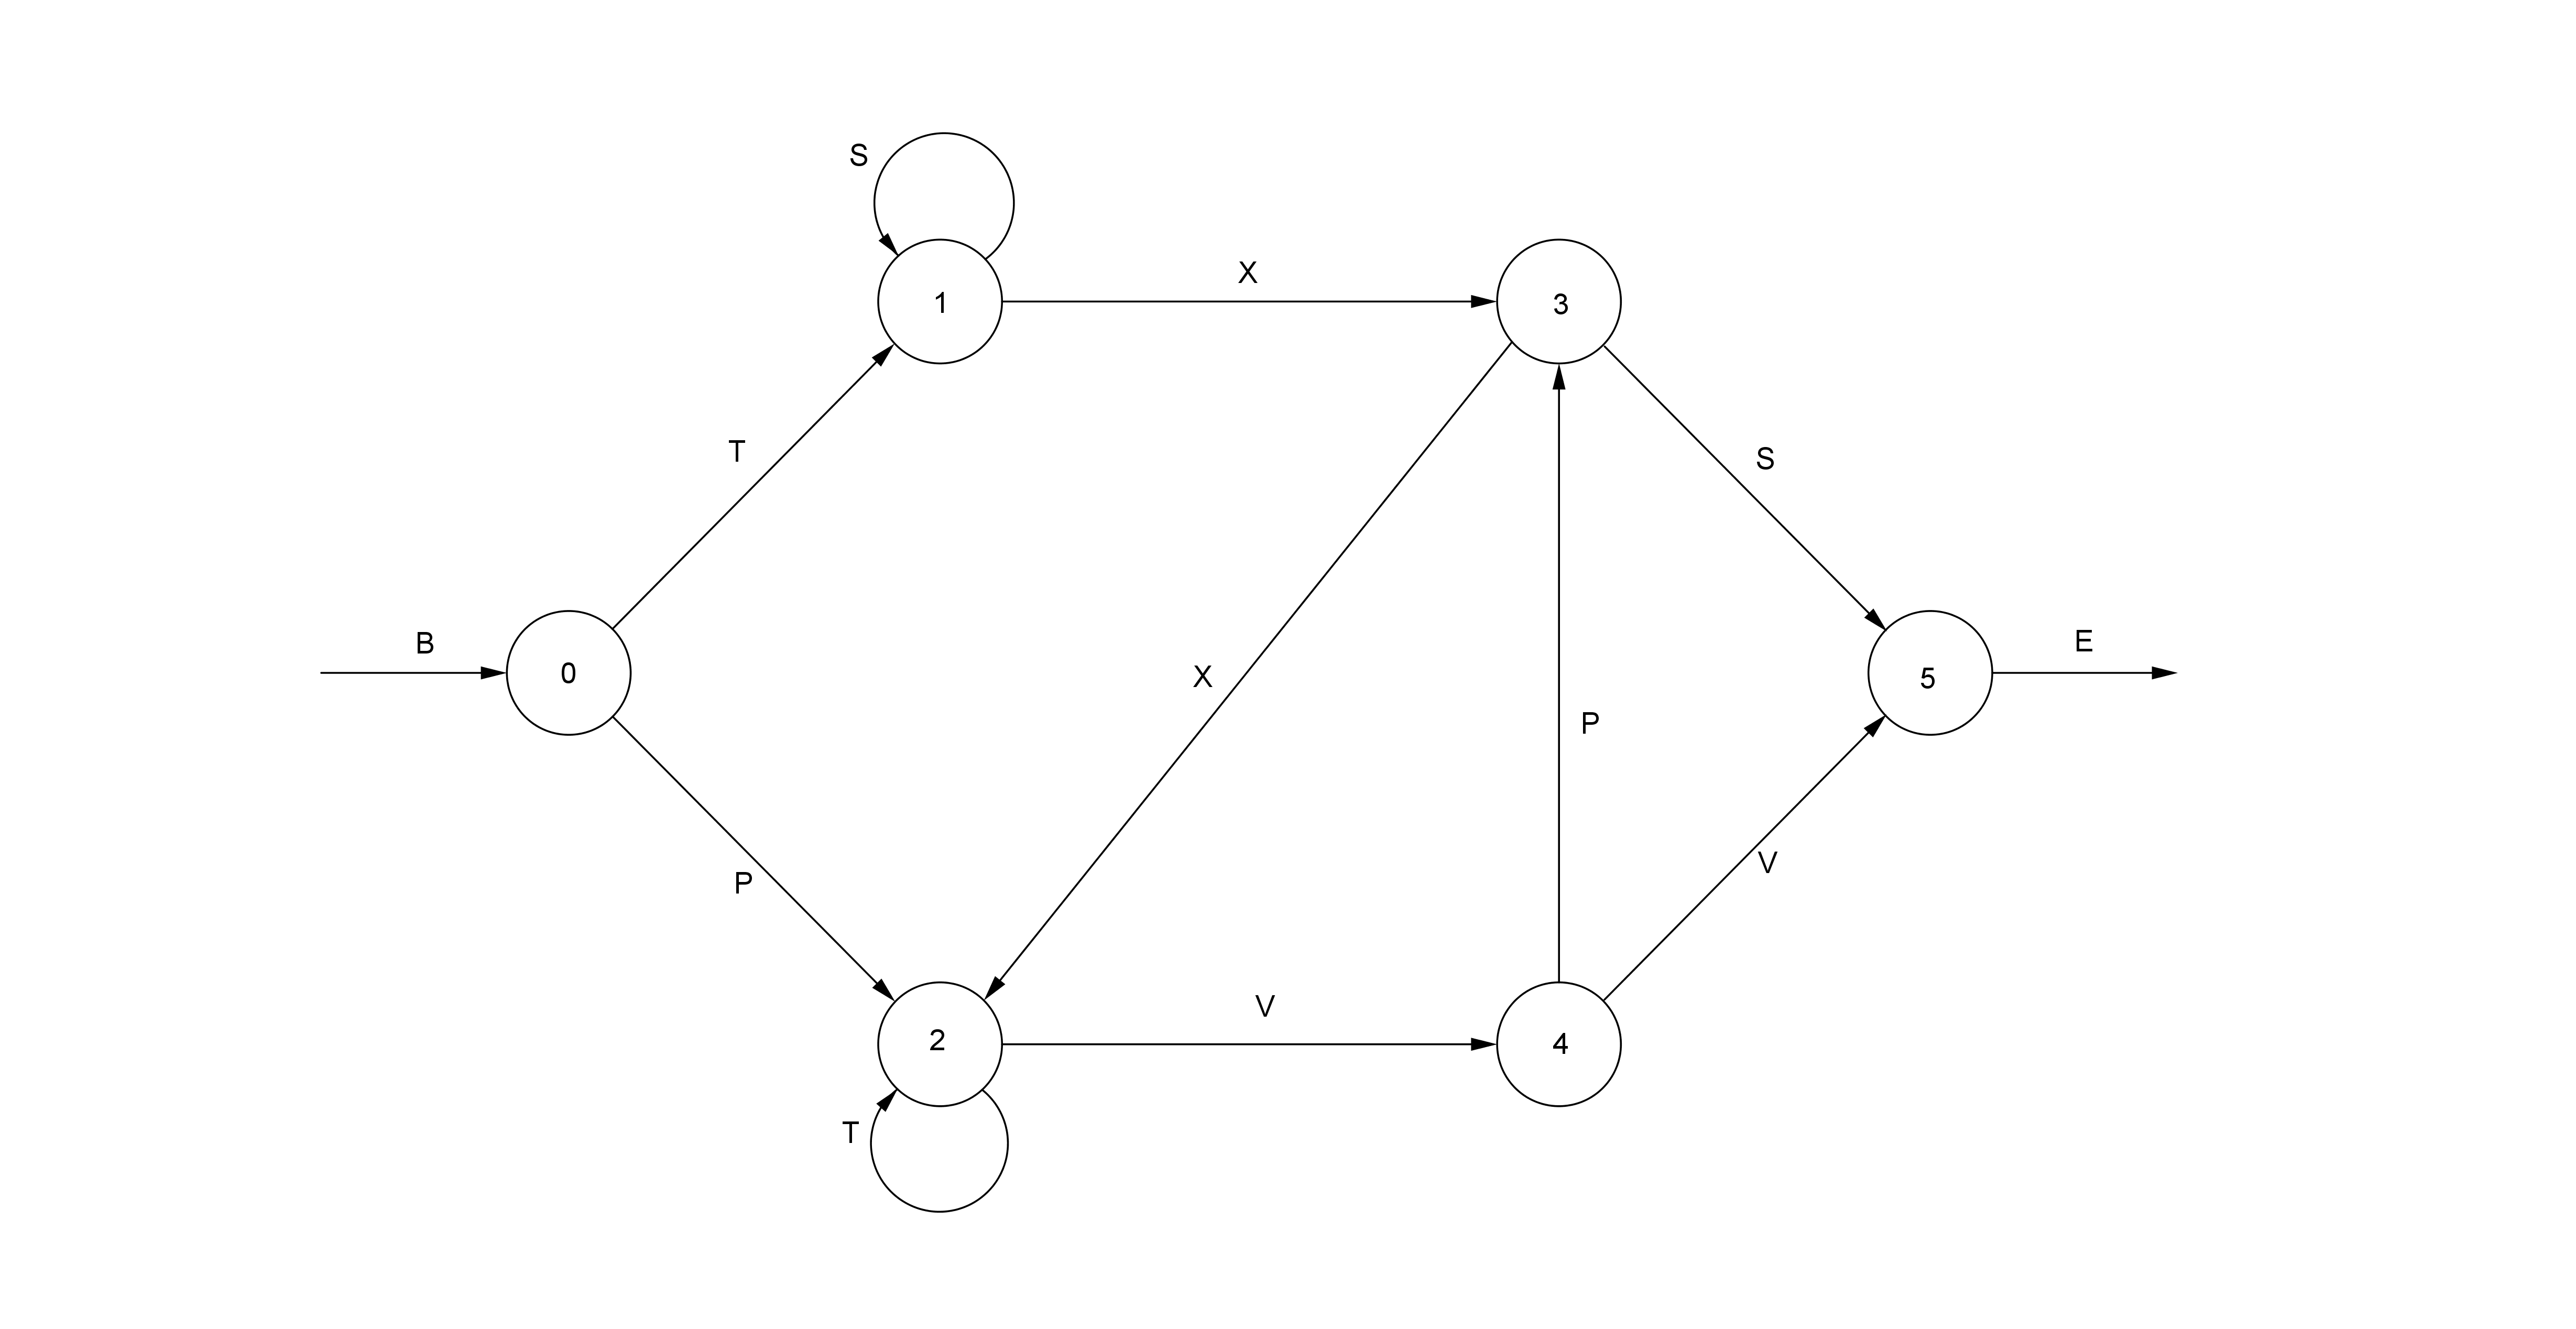
\includegraphics[scale=0.3]{images/reber_simple.png}
\caption{Automate reconnaissant la grammaire de Reber simple}
\label{Grammaire de Reber simple}
\end{center}
\end{figure}

A l'aide de cette automate, nous générerons deux ensembles de mots respectivement afin d'entraîner et de tester notre futur réseau. L'objectif du réseau sera alors d'apprendre cette grammaire afin de prédire les caractères possibles après un caractère donné.

L'étape suivante consistera à tester les algorithmes sur l'apprentissage de la grammaire de Reber symmétrique présentée sur la figure \ref{Grammaire de Reber symétrique}.  
\begin{figure}[h!]
\begin{center}
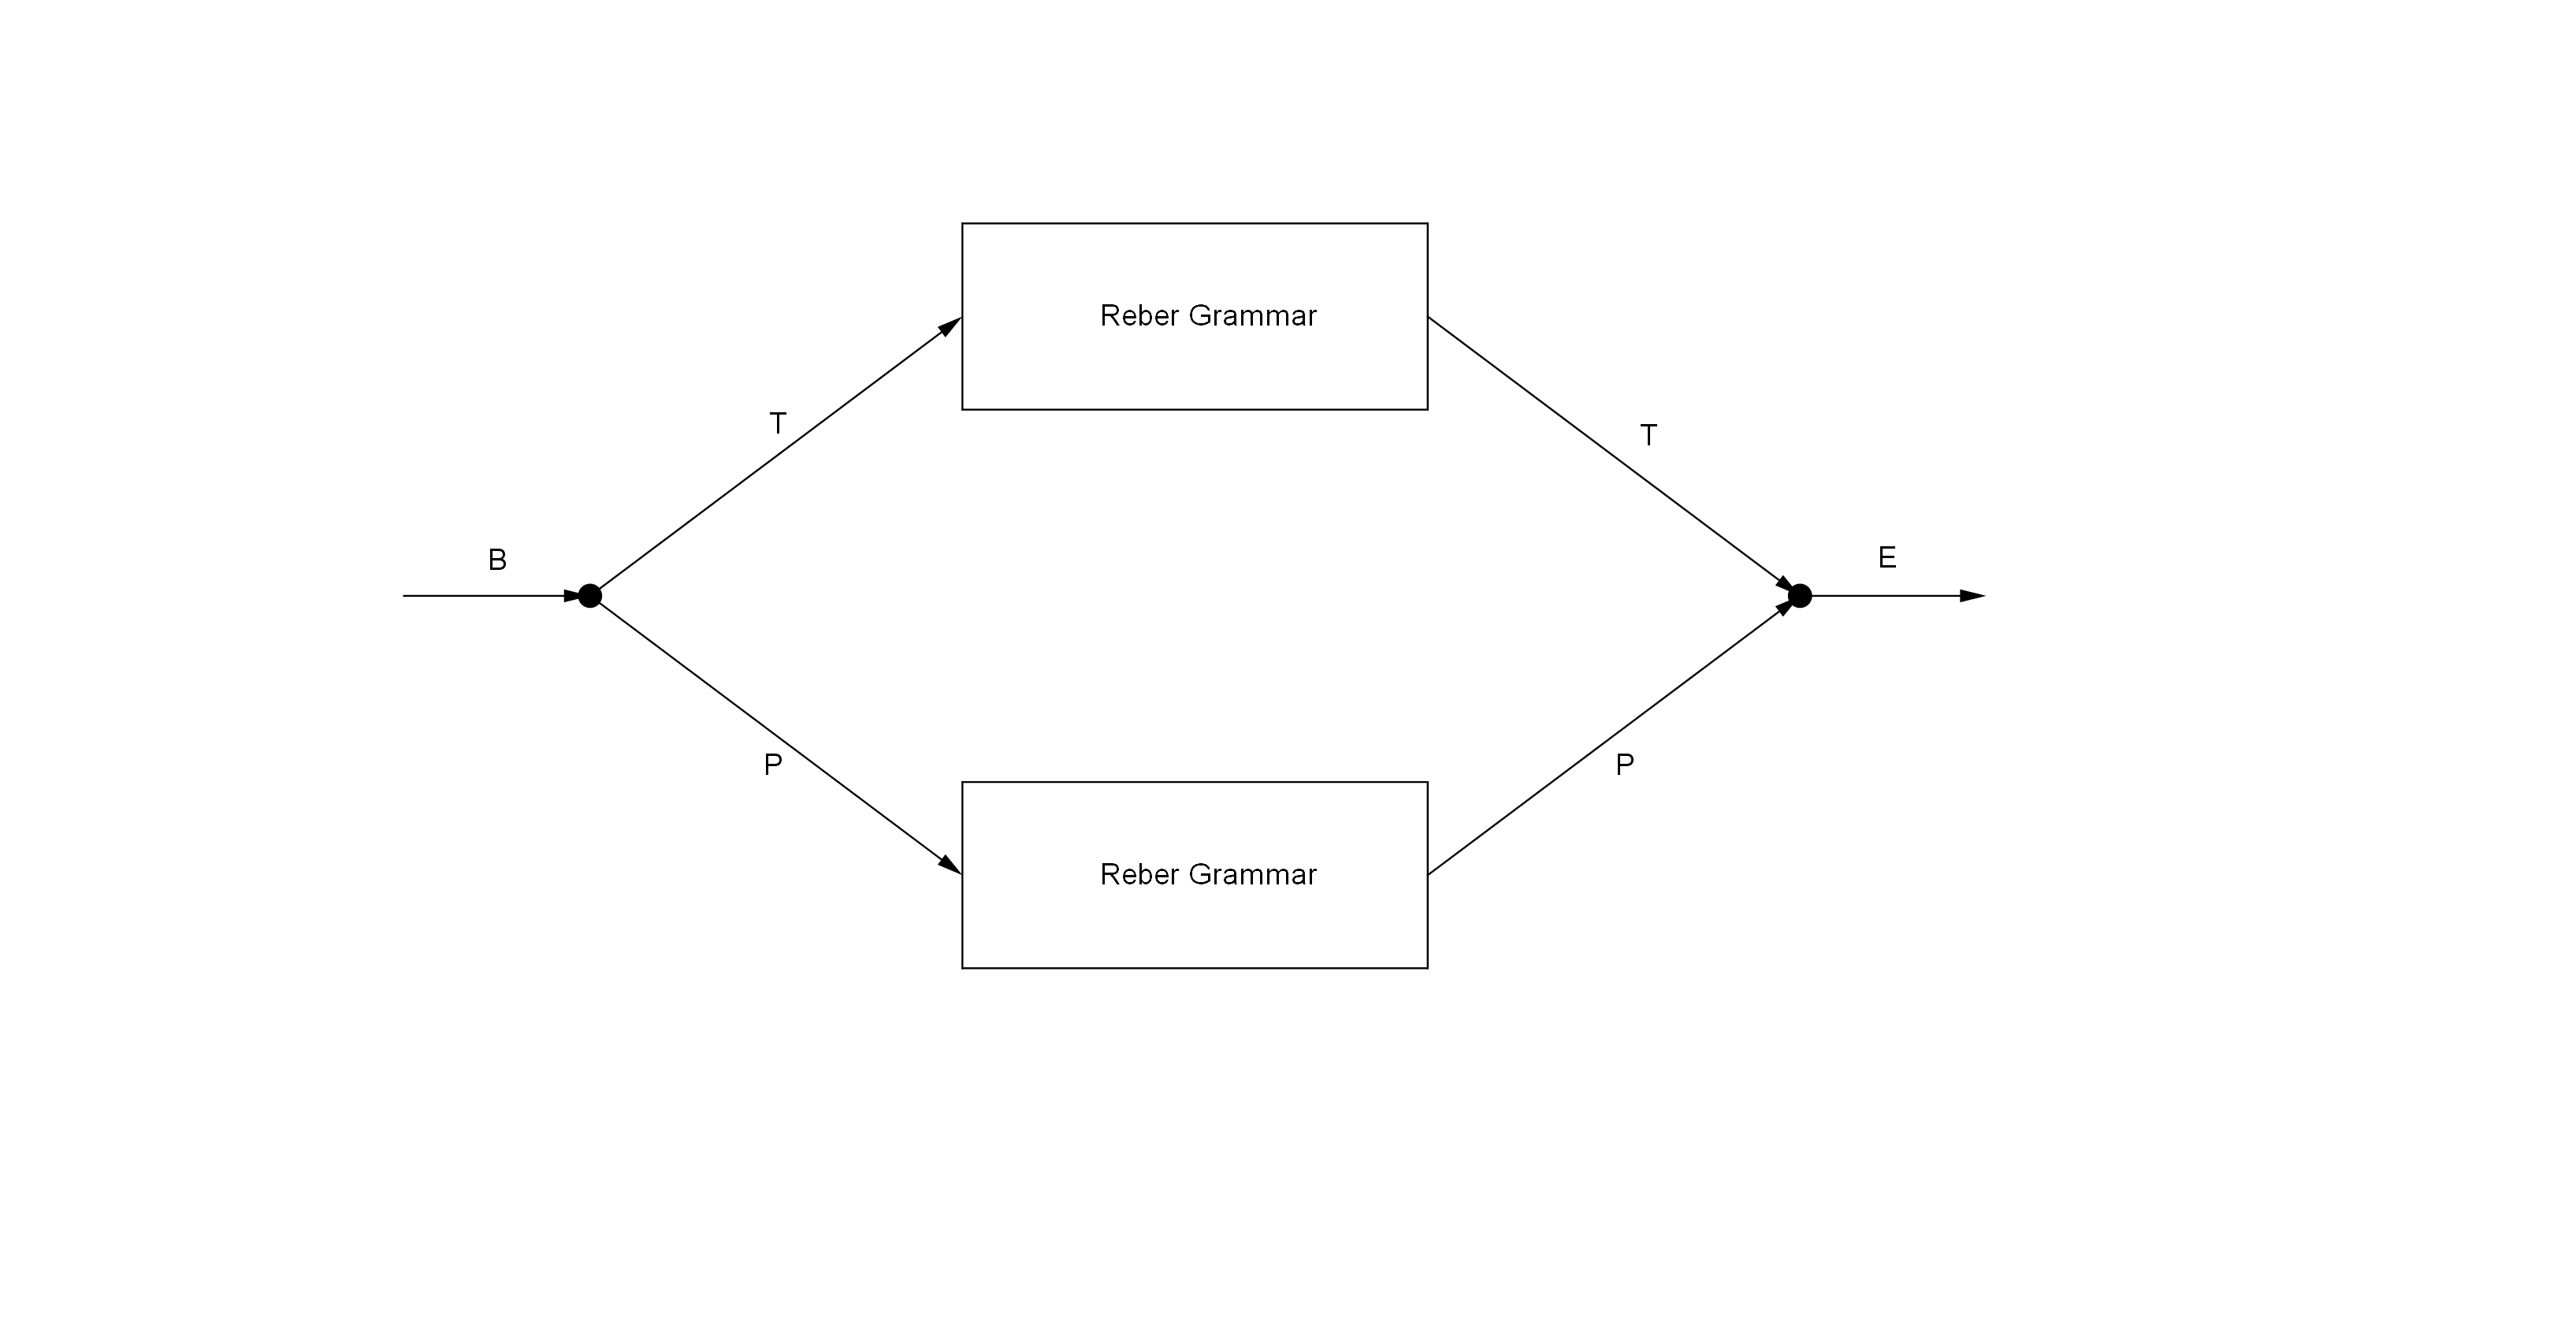
\includegraphics[scale=0.5]{images/reber_symmetrique.png}
\caption{Automate reconnaissant la grammaire de Reber symmétrique}
\label{Grammaire de Reber symmétrique}
\end{center}
\end{figure}

Dans cette situation, le réseau devra être capable de se souvenir d'un état passé (T ou P) afin de prédire le nouvel état (T ou P). Cet état passé pourra être plus ou moins lointain en fonction de la taille de la grammaire de Reber insérée au milieu. 

\section{Comparaison des deux algorithmes}

\section{Problème des dépendances temporelles}
\chapter{Long Short-Term Memory (LSTM)}
\section{Motivation}
Les réseaux de neurones récurrents étudiés jusqu'alors permettent effectivement d'apprendre des suites de séquences. Néanmoins, on observe un phénomène d'oubli se caractérisant par une faible influence des plus vieilles informations sur la sortie actuelle.

Cela est dû à la rétropropagation du gradient. En effet, celle-ci est basée sur la règle de la chaîne qui fait donc apparaître un produit de dérivées de fonctions d'activation. Or si ces dérivées sont supérieures à 1, cette partie du gradient rétropropagé risque d'exploser. A l'inverse, si elles sont inférieures à 1, comme c'est le cas pour la sigmoide dont la dérivée a une valeur maximale de 0
25, cette partie du gradient tend à disparaître lorsque l'on remonte loin dans le temps. Ainsi, on perd la dépendance à long terme.

Nous travaillions jusque là avec des réseaux récurrents comme celui présenté sur la figure \ref{RNN classique} composé d'une simple couche de tangentes hyperboliques.

\begin{figure}[h!]
\begin{center}
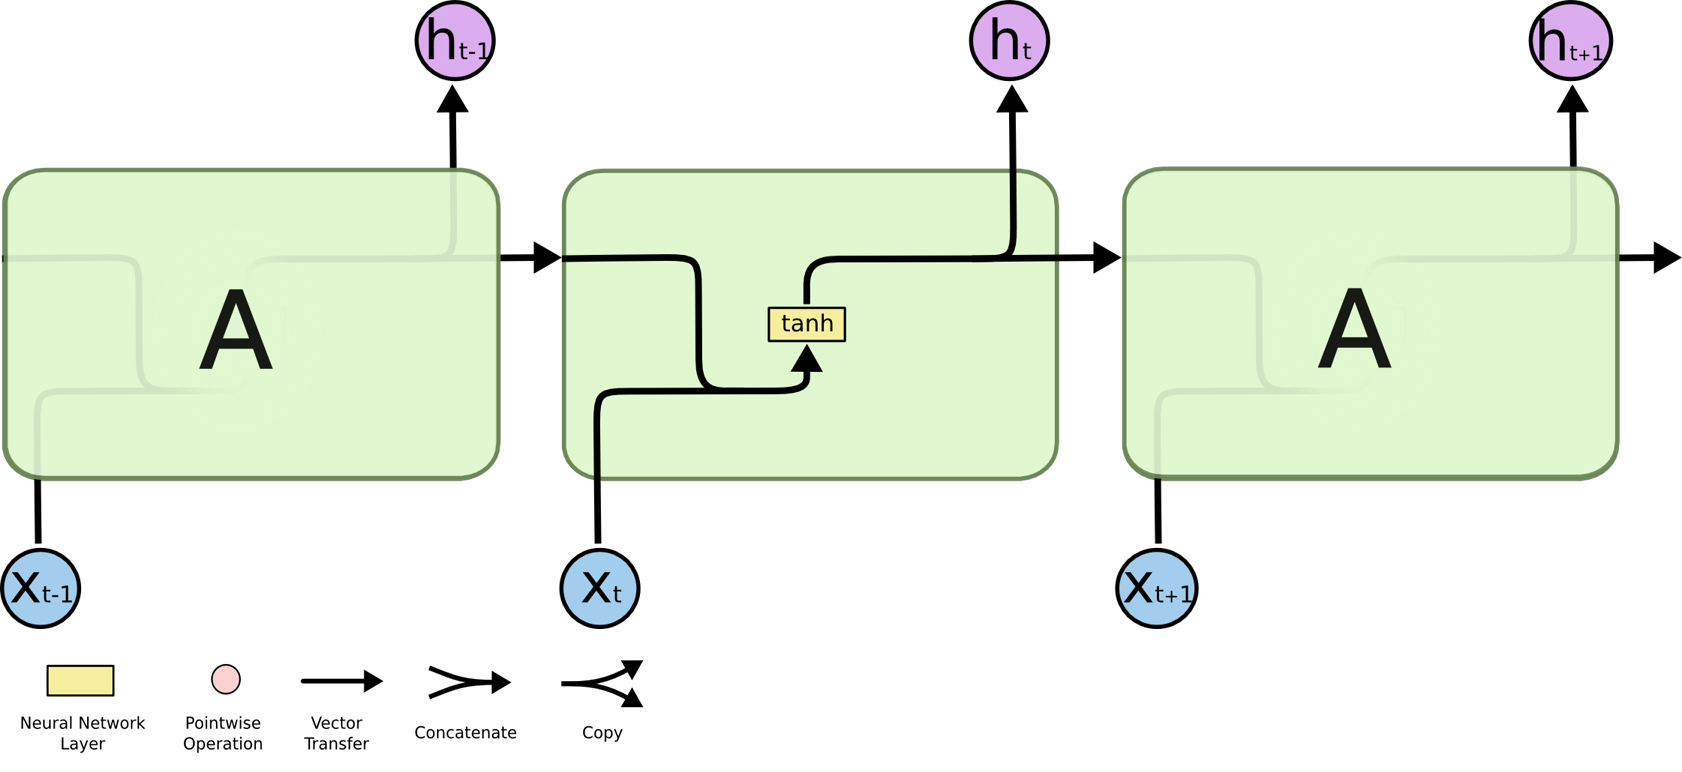
\includegraphics[scale=0.25]{images/chapter6/RNN_classique.png}
\caption{Dépliage d'un RNN classique}
\label{RNN classique}
\end{center}
\end{figure}

Dans le cadre des LSTM, nous utilisons une nouvelle cellule de base afin d'éviter cette disparition du gradient lors de la rétropropagation.

\newpage

\section{Principe de fonctionnement}
Comme pour les réseaux récurrents, on peut déplier les LSTM afin de se ramener à une cellule de base qui se répète. Le principe des LSTM repose sur l'existence d'un état qui apparaît tout en haut de la cellule et qui subit seulement quelques modifications linéaires. Cela permettra ainsi, lors de la rétropropagation du gradient, de ne pas perdre la dépendance avec les informations lointaines.

La cellule de base des LSTM peut donc être représentée par la figure suivante.

\begin{figure}[h!]
\begin{center}
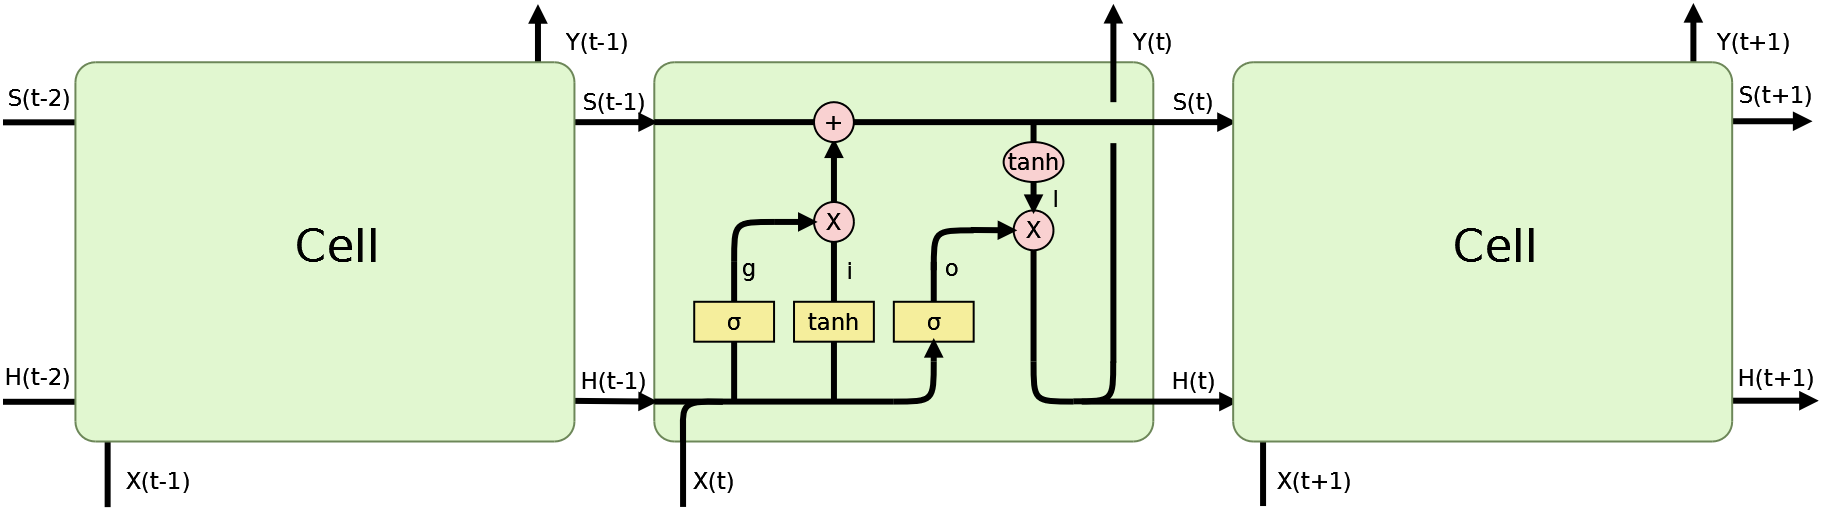
\includegraphics[scale=0.12]{images/chapter6/LSTM_article_plusieurscell.png}
\caption{Cellule élémentaire des LSTM}
\label{cellule LSTM}
\end{center}
\end{figure}

Cette figure permet de représenter facilement le réseau en utilisant la structure d'un graphe de calcul. Il faut cependant bien distinguer les fonctions tanh et sigmoide qui symbolisent une couche entière de neurones (dans les rectangles jaunes) et la fonction tanh (dans le cercle rose) qui s'applique à chaque élément du vecteur en entrée. De même, les multiplications dans les cercles roses se font terme à terme.

Les poids à régler lors de l'apprentissage se situent au niveau de chaque couche de neurones sigmoide et tanh. Il est à noter que lorsque l'on déplie la cellule LSTM dans le temps, les poids sont les mêmes d'une cellule à l'autre. Le fait qu'ils soient ainsi partagés sera important pour l'implémentation.

On peut distinguer plusieurs parties dans la cellule LSTM qui possèdent chacune une fonction particulière.

\begin{figure}[h!]
\begin{center}
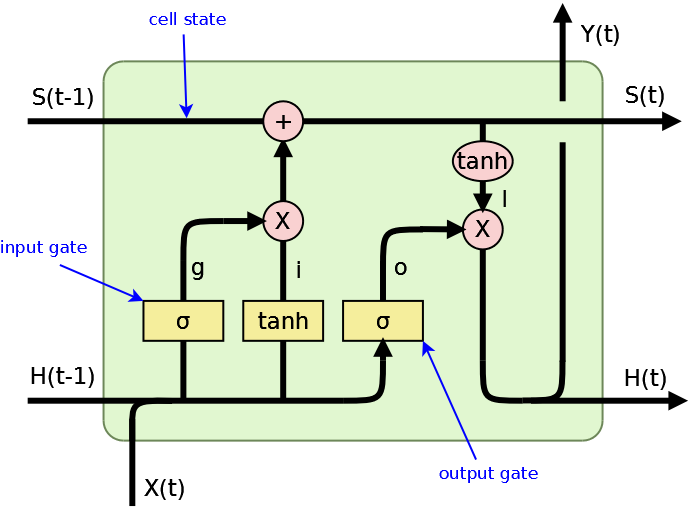
\includegraphics[scale=0.2]{images/chapter6/LSTM_article_gates.png}
\caption{Différentes parties d'une cellule LSTM}
\label{cellule LSTM gates}
\end{center}
\end{figure}

Le cell state S correspond à la mémoire de la cellule. Celle-ci subit peu de modification au cours du temps, correspondant à l'ajout d'information dans la mémoire.

Les sigmoides permettent d'obtenir des sorties comprises entre 0 et 1. On peut donc pondérer l'importance d'une valeur en la multipliant par la sortie d'une sigmoïde. Si la sortie de la sigmoide est proche de 1, cela signifie que l'on garde la valeur, en revanche, si celle-ci est proche de 0, on oublie la valeur calculée.

Ainsi on calcule un vecteur i à partir de l'entrée et de la sortie précédente à l'aide d'une couche de tanh. Puis, on le multiplie terme à terme par le vecteur de sortie g d'une couche de sigmoides appelée input gate afin de sélectionner les informations que l'on souhaite conserver. Enfin, on ajoute ces informations sélectionnées dans le cell state. 

La sortie de la cellule est obtenue à partir du cell state auquel on applique une tanh. Enfin, on sélectionne les informations que l'on veut garder en sortie à l'aide d'une couche de sigmoides appelée output gate appliquée à l'entrée.


En pratique, on n'est pas sûr qu'une cellule LSTM suive effectivement le principe décrit précédemment. Celui-ci est plutôt une illustration afin de comprendre de manière générale le fonctionnement des LSTM.

La structure d'une cellule LSTM n'est pas non figée. En effet, il est possible de l'adapter en ajoutant, enlevant certains éléments, gates. Par exemple, on peut ajouter une forget gate composée d'une couche de sigmoides au début de la cellule. On multiplie la sortie de cette forget gate afin de garder, supprimer, réduire certaines composantes du cell state. 

\break

Dans le cas d'une cellule LSTM, les équations de propagation sont simples à calculer. En effet, comme pour le graphe de calcul, les équations sont directement données par le schéma.

Pour la bakcpropagation du gradient, il est toutefois nécessaire de calculer les formules à utiliser dans l'algorithme. La figure \ref{cellule LSTM gradient} fait apparaître le gradient à chaque endroit de la cellule.

\begin{figure}[h!]
\begin{center}
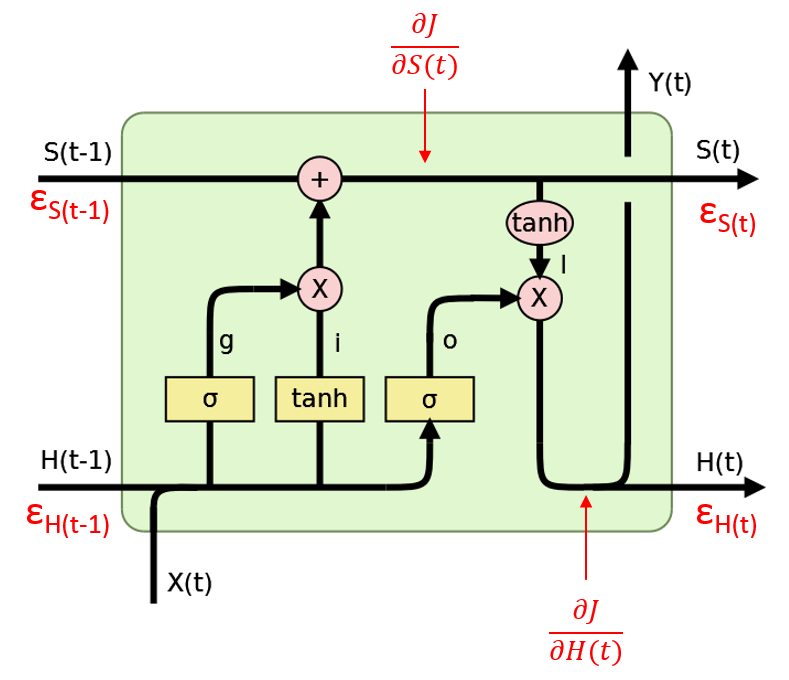
\includegraphics[scale=0.3]{images/chapter6/LSTM_gradient.png}
\caption{Cellule LSTM}
\label{cellule LSTM gradient}
\end{center}
\end{figure}


En utilisant, BPTT pour rétropropager le gradient sur le graphe du LSTM déplié, on obtient les formules suivantes :

\begin{equation}
\varepsilon_{S(t-1)} = \frac{\partial J}{\partial S(t)} = \varepsilon_{S(t)} + F_{l}^{\prime}\text{diag}(o)\frac{\partial J}{\partial H(t)}
\end{equation}

\begin{equation}
\varepsilon_{H(t-1)} = \left((W_{g}^{T}F_{g}^{\prime}\text{diag}(i) + W_{i}^{T}F_{i}^{\prime}\text{diag}(g))\frac{\partial J}{\partial S(t)} + W_{o}^{T}F_{o}^{\prime}\text{diag}(l)\frac{\partial J}{\partial H(t)}\right)_{1,...,n}
\end{equation}

avec :

\[
F_{l}^{\prime} = \text{diag}((1 - l_{i}^{2})_{i=1,...,n})
\]

\[
F_{i}^{\prime} = \text{diag}((1 - i_{i}^{2})_{i=1,...,n})
\]

\[
F_{g}^{\prime} = \text{diag}((g_{i}(1 - g_{i}))_{i=1,...,n})
\]

\[
F_{o}^{\prime} = \text{diag}((o_{i}(1 - o_{i}))_{i=1,...,n})
\]


Il est alors possible de calculer le gradient relatif à chaque matrice de poids.

\begin{equation}
\frac{\partial J}{\partial W_{o}}=
\begin{pmatrix}
H(t-1) \\
x(t)
\end{pmatrix}
\left(F_{o}^{\prime}\text{diag}(l)\frac{\partial J}{\partial H(t)}\right)^{T}
\end{equation}

\begin{equation}
\frac{\partial J}{\partial W_{i}}=
\begin{pmatrix}
H(t-1) \\
x(t)
\end{pmatrix}
\left(F_{i}^{\prime}\text{diag}(g)\frac{\partial J}{\partial S(t)}\right)^{T}
\end{equation}

\begin{equation}
\frac{\partial J}{\partial W_{g}}=
\begin{pmatrix}
H(t-1) \\
x(t)
\end{pmatrix}
\left(F_{g}^{\prime}\text{diag}(i)\frac{\partial J}{\partial S(t)}\right)^{T}
\end{equation}

On rétropropage le gradient dans tout le graphe déplié avec les formules précédentes. Celui-ci est à chaque fois accumulé au niveau des poids. Les poids $W_{o}$, $W_{i}$ et $W_{g}$ sont alors mis à jour avec la formule :

\begin{equation}
W = W - \eta \sum{\frac{\partial J}{\partial W}}
\end{equation} 

\section{Première Implémentation}

Une première implémentation des LSTM a été réalisé en conservant le plus possible le concept de cellule indépendante. Ainsi une classe Weights contient tous les poids de la cellule et la classe Lstmcell se contentera elle de calculer la propagation et la rétropropagation (Voir Figure 4.4 de la cellule LSTM pour situer les poids).

Si cette implémentation intuitive fonctionne et donne des résultats satisfaisants, elle n'est cependant pas très adapté à la création de réseaux de cellules LSTM. C'est pour cela que nous nous sommes lancés dans une seconde implémentation, plus pratique et flexible.

\begin{figure}[h!]
\begin{center}
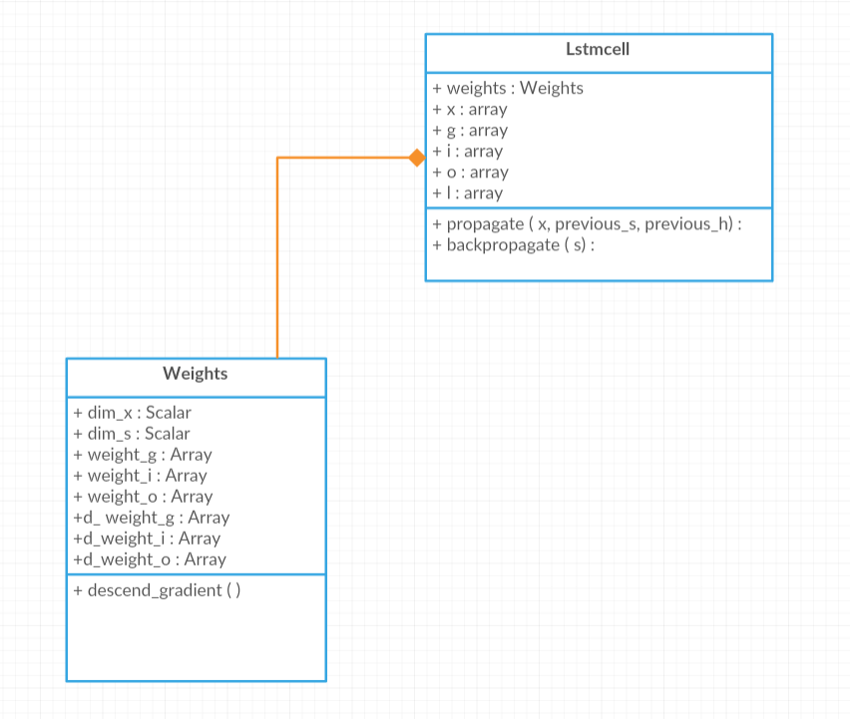
\includegraphics[scale=0.8]{images/chapter6/UML_LSTM_Implementation_1.png}
\caption{Diagramme UML de la cellule LSTM}
\label{cellule LSTM UML 1}
\end{center}
\end{figure}

\section{Implémentation avec des nœuds}

Cette seconde implémentation a pour but de réutiliser \texttt{pychain}, la librairie de graphes de calculs que nous avons développée et déjà appliquée aux réseaux feedforward et aux réseaux récurrents. L'utilisation des graphes de calculs nous permettra d'optimiser les calculs mais surtout de gagner en flexibilité. En effet, on pourra alors facilement changer l'architecture de la cellule LSTM mais aussi très simplement combiner plusieurs cellules entre elles. Ou même combiner des cellules LSTM avec des réseaux feedforward.

L'objectif est de créer un n\oe{}ud à trois entrées et à deux sorties comme décrit sur la figure \ref{lstm_node_macro}.

\begin{figure}[h!]
\begin{center}
% Graphic for TeX using PGF
% Title: /home/pierre/Programming/pl-lstm/slides/images/node_lstm.dia
% Creator: Dia v0.97.3
% CreationDate: Wed Mar  8 21:09:21 2017
% For: pierre
% \usepackage{tikz}
% The following commands are not supported in PSTricks at present
% We define them conditionally, so when they are implemented,
% this pgf file will use them.
\ifx\du\undefined
  \newlength{\du}
\fi
\setlength{\du}{15\unitlength}
\begin{tikzpicture}
\pgftransformxscale{1.000000}
\pgftransformyscale{-1.000000}
\definecolor{dialinecolor}{rgb}{0.000000, 0.000000, 0.000000}
\pgfsetstrokecolor{dialinecolor}
\definecolor{dialinecolor}{rgb}{1.000000, 1.000000, 1.000000}
\pgfsetfillcolor{dialinecolor}
\definecolor{dialinecolor}{rgb}{1.000000, 1.000000, 1.000000}
\pgfsetfillcolor{dialinecolor}
\pgfpathellipse{\pgfpoint{11.500000\du}{4.000000\du}}{\pgfpoint{1.500000\du}{0\du}}{\pgfpoint{0\du}{1.500000\du}}
\pgfusepath{fill}
\pgfsetlinewidth{0.100000\du}
\pgfsetdash{}{0pt}
\pgfsetdash{}{0pt}
\definecolor{dialinecolor}{rgb}{0.000000, 0.000000, 0.000000}
\pgfsetstrokecolor{dialinecolor}
\pgfpathellipse{\pgfpoint{11.500000\du}{4.000000\du}}{\pgfpoint{1.500000\du}{0\du}}{\pgfpoint{0\du}{1.500000\du}}
\pgfusepath{stroke}
\pgfsetlinewidth{0.100000\du}
\pgfsetdash{}{0pt}
\pgfsetdash{}{0pt}
\pgfsetbuttcap
{
\definecolor{dialinecolor}{rgb}{0.000000, 0.000000, 0.000000}
\pgfsetfillcolor{dialinecolor}
% was here!!!
\pgfsetarrowsend{latex}
\definecolor{dialinecolor}{rgb}{0.000000, 0.000000, 0.000000}
\pgfsetstrokecolor{dialinecolor}
\draw (7.500000\du,5.500000\du)--(10.048340\du,4.544373\du);
}
\pgfsetlinewidth{0.100000\du}
\pgfsetdash{}{0pt}
\pgfsetdash{}{0pt}
\pgfsetbuttcap
{
\definecolor{dialinecolor}{rgb}{0.000000, 0.000000, 0.000000}
\pgfsetfillcolor{dialinecolor}
% was here!!!
\pgfsetarrowsend{latex}
\definecolor{dialinecolor}{rgb}{0.000000, 0.000000, 0.000000}
\pgfsetstrokecolor{dialinecolor}
\draw (7.500000\du,4.000000\du)--(9.951172\du,4.000000\du);
}
\pgfsetlinewidth{0.100000\du}
\pgfsetdash{}{0pt}
\pgfsetdash{}{0pt}
\pgfsetbuttcap
{
\definecolor{dialinecolor}{rgb}{0.000000, 0.000000, 0.000000}
\pgfsetfillcolor{dialinecolor}
% was here!!!
\pgfsetarrowsend{latex}
\definecolor{dialinecolor}{rgb}{0.000000, 0.000000, 0.000000}
\pgfsetstrokecolor{dialinecolor}
\draw (13.000000\du,4.000000\du)--(15.500000\du,3.000000\du);
}
% setfont left to latex
\definecolor{dialinecolor}{rgb}{0.000000, 0.000000, 0.000000}
\pgfsetstrokecolor{dialinecolor}
\node[anchor=west] at (6.500000\du,2.500000\du){$x$};
% setfont left to latex
\definecolor{dialinecolor}{rgb}{0.000000, 0.000000, 0.000000}
\pgfsetstrokecolor{dialinecolor}
\node[anchor=west] at (6.500000\du,4.000000\du){$h_{in}$};
% setfont left to latex
\definecolor{dialinecolor}{rgb}{0.000000, 0.000000, 0.000000}
\pgfsetstrokecolor{dialinecolor}
\node[anchor=west] at (6.500000\du,5.500000\du){$s_{in}$};
% setfont left to latex
\definecolor{dialinecolor}{rgb}{0.000000, 0.000000, 0.000000}
\pgfsetstrokecolor{dialinecolor}
\node at (11.500000\du,4.222500\du){LSTM};
\pgfsetlinewidth{0.100000\du}
\pgfsetdash{}{0pt}
\pgfsetdash{}{0pt}
\pgfsetbuttcap
{
\definecolor{dialinecolor}{rgb}{0.000000, 0.000000, 0.000000}
\pgfsetfillcolor{dialinecolor}
% was here!!!
\pgfsetarrowsend{latex}
\definecolor{dialinecolor}{rgb}{0.000000, 0.000000, 0.000000}
\pgfsetstrokecolor{dialinecolor}
\draw (7.500000\du,2.500000\du)--(10.048340\du,3.455627\du);
}
% setfont left to latex
\definecolor{dialinecolor}{rgb}{0.000000, 0.000000, 0.000000}
\pgfsetstrokecolor{dialinecolor}
\node[anchor=west] at (7.000000\du,2.500000\du){};
% setfont left to latex
\definecolor{dialinecolor}{rgb}{0.000000, 0.000000, 0.000000}
\pgfsetstrokecolor{dialinecolor}
\node[anchor=west] at (15.500000\du,3.000000\du){$h_{out}$};
\pgfsetlinewidth{0.100000\du}
\pgfsetdash{}{0pt}
\pgfsetdash{}{0pt}
\pgfsetbuttcap
{
\definecolor{dialinecolor}{rgb}{0.000000, 0.000000, 0.000000}
\pgfsetfillcolor{dialinecolor}
% was here!!!
\pgfsetarrowsend{latex}
\definecolor{dialinecolor}{rgb}{0.000000, 0.000000, 0.000000}
\pgfsetstrokecolor{dialinecolor}
\draw (13.000000\du,4.000000\du)--(15.500000\du,5.000000\du);
}
% setfont left to latex
\definecolor{dialinecolor}{rgb}{0.000000, 0.000000, 0.000000}
\pgfsetstrokecolor{dialinecolor}
\node[anchor=west] at (15.500000\du,5.000000\du){$s_{out}$};
\end{tikzpicture}

\caption{Architecture macroscopique de la cellule LSTM.}
\label{lstm_node_macro}
\end{center}
\end{figure}

Deux solutions s'offraient à nous. On pouvait réutiliser les équations de propagation et de rétropropagation décrite dans la section précédente. Cette solution a l'inconvénient qu'il est nécessaire de dériver à la main les formules de propagation et de rétropropagation à chaque fois que l'on veut changer l'architecture de la cellule LSTM. On n'atteint donc pas l'objectif de flexibilité.

L'autre solution consiste à exprimer le n\oe{}ud LSTM en fonction d'autres n\oe{}uds élémentaires que nous avons définis dans la partie \ref{comp_graph_part}. Comme cela, le gradient sera calculé automatiquement par les n\oe{}uds. Afin de créer un tel n\oe{}uds, nous avons défini une classe \textit{CompositeNode} qui est basée sur le design pattern Composite. Il s'agit d'une classe fille de la classe \textit{Node} qui a comme attributs d'autres n\oe{}uds. La classe \textit{LSTMNode} est alors une classe fille de la classe \textit{CompositeNode}.

La figure \ref{lstm_node_micro} présente les n\oe{}uds qui composent la cellule LSTM ainsi définie.

\begin{figure}[h!]
\begin{center}
% Graphic for TeX using PGF
% Title: /home/pierre/Programming/pl-lstm/images/illustrations_cr/lstm_node.dia
% Creator: Dia v0.97.3
% CreationDate: Wed Mar  8 22:05:31 2017
% For: pierre
% \usepackage{tikz}
% The following commands are not supported in PSTricks at present
% We define them conditionally, so when they are implemented,
% this pgf file will use them.
\ifx\du\undefined
  \newlength{\du}
\fi
\setlength{\du}{15\unitlength}
\begin{tikzpicture}[scale=0.4]
\pgftransformxscale{1.000000}
\pgftransformyscale{-1.000000}
\definecolor{dialinecolor}{rgb}{0.000000, 0.000000, 0.000000}
\pgfsetstrokecolor{dialinecolor}
\definecolor{dialinecolor}{rgb}{1.000000, 1.000000, 1.000000}
\pgfsetfillcolor{dialinecolor}
\pgfsetlinewidth{0.100000\du}
\pgfsetdash{}{0pt}
\pgfsetdash{}{0pt}
\pgfsetmiterjoin
\definecolor{dialinecolor}{rgb}{1.000000, 1.000000, 1.000000}
\pgfsetfillcolor{dialinecolor}
\fill (5.000000\du,-11.000000\du)--(5.000000\du,20.000000\du)--(53.000000\du,20.000000\du)--(53.000000\du,-11.000000\du)--cycle;
\definecolor{dialinecolor}{rgb}{0.000000, 0.000000, 0.000000}
\pgfsetstrokecolor{dialinecolor}
\draw (5.000000\du,-11.000000\du)--(5.000000\du,20.000000\du)--(53.000000\du,20.000000\du)--(53.000000\du,-11.000000\du)--cycle;
\pgfsetlinewidth{0.100000\du}
\pgfsetdash{}{0pt}
\pgfsetdash{}{0pt}
\pgfsetbuttcap
{
\definecolor{dialinecolor}{rgb}{0.000000, 0.000000, 0.000000}
\pgfsetfillcolor{dialinecolor}
% was here!!!
\pgfsetarrowsend{latex}
\definecolor{dialinecolor}{rgb}{0.000000, 0.000000, 0.000000}
\pgfsetstrokecolor{dialinecolor}
\draw (0.000000\du,-8.500000\du)--(5.000000\du,-8.500000\du);
}
\pgfsetlinewidth{0.100000\du}
\pgfsetdash{}{0pt}
\pgfsetdash{}{0pt}
\pgfsetbuttcap
{
\definecolor{dialinecolor}{rgb}{0.000000, 0.000000, 0.000000}
\pgfsetfillcolor{dialinecolor}
% was here!!!
\pgfsetarrowsend{latex}
\definecolor{dialinecolor}{rgb}{0.000000, 0.000000, 0.000000}
\pgfsetstrokecolor{dialinecolor}
\draw (0.000000\du,11.500000\du)--(5.000000\du,11.500000\du);
}
\pgfsetlinewidth{0.100000\du}
\pgfsetdash{}{0pt}
\pgfsetdash{}{0pt}
\pgfsetbuttcap
{
\definecolor{dialinecolor}{rgb}{0.000000, 0.000000, 0.000000}
\pgfsetfillcolor{dialinecolor}
% was here!!!
\pgfsetarrowsend{latex}
\definecolor{dialinecolor}{rgb}{0.000000, 0.000000, 0.000000}
\pgfsetstrokecolor{dialinecolor}
\draw (53.000000\du,-8.500000\du)--(58.000000\du,-8.500000\du);
}
\pgfsetlinewidth{0.100000\du}
\pgfsetdash{}{0pt}
\pgfsetdash{}{0pt}
\pgfsetbuttcap
{
\definecolor{dialinecolor}{rgb}{0.000000, 0.000000, 0.000000}
\pgfsetfillcolor{dialinecolor}
% was here!!!
\pgfsetarrowsend{latex}
\definecolor{dialinecolor}{rgb}{0.000000, 0.000000, 0.000000}
\pgfsetstrokecolor{dialinecolor}
\draw (53.000000\du,11.500000\du)--(58.000000\du,11.500000\du);
}
\pgfsetlinewidth{0.100000\du}
\pgfsetdash{}{0pt}
\pgfsetdash{}{0pt}
\pgfsetbuttcap
{
\definecolor{dialinecolor}{rgb}{0.000000, 0.000000, 0.000000}
\pgfsetfillcolor{dialinecolor}
% was here!!!
\pgfsetarrowsend{latex}
\definecolor{dialinecolor}{rgb}{0.000000, 0.000000, 0.000000}
\pgfsetstrokecolor{dialinecolor}
\draw (13.500000\du,25.000000\du)--(13.500000\du,20.000000\du);
}
\definecolor{dialinecolor}{rgb}{1.000000, 1.000000, 1.000000}
\pgfsetfillcolor{dialinecolor}
\pgfpathellipse{\pgfpoint{19.500000\du}{5.500000\du}}{\pgfpoint{1.500000\du}{0\du}}{\pgfpoint{0\du}{1.500000\du}}
\pgfusepath{fill}
\pgfsetlinewidth{0.100000\du}
\pgfsetdash{}{0pt}
\pgfsetdash{}{0pt}
\definecolor{dialinecolor}{rgb}{0.000000, 0.000000, 0.000000}
\pgfsetstrokecolor{dialinecolor}
\pgfpathellipse{\pgfpoint{19.500000\du}{5.500000\du}}{\pgfpoint{1.500000\du}{0\du}}{\pgfpoint{0\du}{1.500000\du}}
\pgfusepath{stroke}
\definecolor{dialinecolor}{rgb}{1.000000, 1.000000, 1.000000}
\pgfsetfillcolor{dialinecolor}
\pgfpathellipse{\pgfpoint{13.500000\du}{5.500000\du}}{\pgfpoint{1.500000\du}{0\du}}{\pgfpoint{0\du}{1.500000\du}}
\pgfusepath{fill}
\pgfsetlinewidth{0.100000\du}
\pgfsetdash{}{0pt}
\pgfsetdash{}{0pt}
\definecolor{dialinecolor}{rgb}{0.000000, 0.000000, 0.000000}
\pgfsetstrokecolor{dialinecolor}
\pgfpathellipse{\pgfpoint{13.500000\du}{5.500000\du}}{\pgfpoint{1.500000\du}{0\du}}{\pgfpoint{0\du}{1.500000\du}}
\pgfusepath{stroke}
\definecolor{dialinecolor}{rgb}{1.000000, 1.000000, 1.000000}
\pgfsetfillcolor{dialinecolor}
\pgfpathellipse{\pgfpoint{13.500000\du}{17.500000\du}}{\pgfpoint{1.500000\du}{0\du}}{\pgfpoint{0\du}{1.500000\du}}
\pgfusepath{fill}
\pgfsetlinewidth{0.100000\du}
\pgfsetdash{}{0pt}
\pgfsetdash{}{0pt}
\definecolor{dialinecolor}{rgb}{0.000000, 0.000000, 0.000000}
\pgfsetstrokecolor{dialinecolor}
\pgfpathellipse{\pgfpoint{13.500000\du}{17.500000\du}}{\pgfpoint{1.500000\du}{0\du}}{\pgfpoint{0\du}{1.500000\du}}
\pgfusepath{stroke}
\definecolor{dialinecolor}{rgb}{1.000000, 1.000000, 1.000000}
\pgfsetfillcolor{dialinecolor}
\pgfpathellipse{\pgfpoint{13.500000\du}{11.500000\du}}{\pgfpoint{1.500000\du}{0\du}}{\pgfpoint{0\du}{1.500000\du}}
\pgfusepath{fill}
\pgfsetlinewidth{0.100000\du}
\pgfsetdash{}{0pt}
\pgfsetdash{}{0pt}
\definecolor{dialinecolor}{rgb}{0.000000, 0.000000, 0.000000}
\pgfsetstrokecolor{dialinecolor}
\pgfpathellipse{\pgfpoint{13.500000\du}{11.500000\du}}{\pgfpoint{1.500000\du}{0\du}}{\pgfpoint{0\du}{1.500000\du}}
\pgfusepath{stroke}
\definecolor{dialinecolor}{rgb}{1.000000, 1.000000, 1.000000}
\pgfsetfillcolor{dialinecolor}
\pgfpathellipse{\pgfpoint{7.500000\du}{11.500000\du}}{\pgfpoint{1.500000\du}{0\du}}{\pgfpoint{0\du}{1.500000\du}}
\pgfusepath{fill}
\pgfsetlinewidth{0.100000\du}
\pgfsetdash{}{0pt}
\pgfsetdash{}{0pt}
\definecolor{dialinecolor}{rgb}{0.000000, 0.000000, 0.000000}
\pgfsetstrokecolor{dialinecolor}
\pgfpathellipse{\pgfpoint{7.500000\du}{11.500000\du}}{\pgfpoint{1.500000\du}{0\du}}{\pgfpoint{0\du}{1.500000\du}}
\pgfusepath{stroke}
\pgfsetlinewidth{0.100000\du}
\pgfsetdash{}{0pt}
\pgfsetdash{}{0pt}
\pgfsetbuttcap
{
\definecolor{dialinecolor}{rgb}{0.000000, 0.000000, 0.000000}
\pgfsetfillcolor{dialinecolor}
% was here!!!
\pgfsetarrowsend{latex}
\definecolor{dialinecolor}{rgb}{0.000000, 0.000000, 0.000000}
\pgfsetstrokecolor{dialinecolor}
\draw (13.500000\du,15.949829\du)--(13.500000\du,13.050171\du);
}
\pgfsetlinewidth{0.100000\du}
\pgfsetdash{}{0pt}
\pgfsetdash{}{0pt}
\pgfsetbuttcap
{
\definecolor{dialinecolor}{rgb}{0.000000, 0.000000, 0.000000}
\pgfsetfillcolor{dialinecolor}
% was here!!!
\pgfsetarrowsend{latex}
\definecolor{dialinecolor}{rgb}{0.000000, 0.000000, 0.000000}
\pgfsetstrokecolor{dialinecolor}
\draw (9.050171\du,11.500000\du)--(11.949829\du,11.500000\du);
}
\pgfsetlinewidth{0.100000\du}
\pgfsetdash{}{0pt}
\pgfsetdash{}{0pt}
\pgfsetmiterjoin
\pgfsetbuttcap
{
\definecolor{dialinecolor}{rgb}{0.000000, 0.000000, 0.000000}
\pgfsetfillcolor{dialinecolor}
% was here!!!
\pgfsetarrowsend{latex}
{\pgfsetcornersarced{\pgfpoint{0.000000\du}{0.000000\du}}\definecolor{dialinecolor}{rgb}{0.000000, 0.000000, 0.000000}
\pgfsetstrokecolor{dialinecolor}
\draw (15.000000\du,11.500000\du)--(15.000000\du,11.500000\du)--(19.500000\du,11.500000\du)--(19.500000\du,7.050171\du);
}}
\pgfsetlinewidth{0.100000\du}
\pgfsetdash{}{0pt}
\pgfsetdash{}{0pt}
\pgfsetbuttcap
{
\definecolor{dialinecolor}{rgb}{0.000000, 0.000000, 0.000000}
\pgfsetfillcolor{dialinecolor}
% was here!!!
\pgfsetarrowsend{latex}
\definecolor{dialinecolor}{rgb}{0.000000, 0.000000, 0.000000}
\pgfsetstrokecolor{dialinecolor}
\draw (15.050171\du,5.500000\du)--(17.949829\du,5.500000\du);
}
\definecolor{dialinecolor}{rgb}{1.000000, 1.000000, 1.000000}
\pgfsetfillcolor{dialinecolor}
\pgfpathellipse{\pgfpoint{29.500000\du}{5.500000\du}}{\pgfpoint{1.500000\du}{0\du}}{\pgfpoint{0\du}{1.500000\du}}
\pgfusepath{fill}
\pgfsetlinewidth{0.100000\du}
\pgfsetdash{}{0pt}
\pgfsetdash{}{0pt}
\definecolor{dialinecolor}{rgb}{0.000000, 0.000000, 0.000000}
\pgfsetstrokecolor{dialinecolor}
\pgfpathellipse{\pgfpoint{29.500000\du}{5.500000\du}}{\pgfpoint{1.500000\du}{0\du}}{\pgfpoint{0\du}{1.500000\du}}
\pgfusepath{stroke}
\definecolor{dialinecolor}{rgb}{1.000000, 1.000000, 1.000000}
\pgfsetfillcolor{dialinecolor}
\pgfpathellipse{\pgfpoint{23.500000\du}{5.500000\du}}{\pgfpoint{1.500000\du}{0\du}}{\pgfpoint{0\du}{1.500000\du}}
\pgfusepath{fill}
\pgfsetlinewidth{0.100000\du}
\pgfsetdash{}{0pt}
\pgfsetdash{}{0pt}
\definecolor{dialinecolor}{rgb}{0.000000, 0.000000, 0.000000}
\pgfsetstrokecolor{dialinecolor}
\pgfpathellipse{\pgfpoint{23.500000\du}{5.500000\du}}{\pgfpoint{1.500000\du}{0\du}}{\pgfpoint{0\du}{1.500000\du}}
\pgfusepath{stroke}
\pgfsetlinewidth{0.100000\du}
\pgfsetdash{}{0pt}
\pgfsetdash{}{0pt}
\pgfsetbuttcap
{
\definecolor{dialinecolor}{rgb}{0.000000, 0.000000, 0.000000}
\pgfsetfillcolor{dialinecolor}
% was here!!!
\pgfsetarrowsstart{latex}
\definecolor{dialinecolor}{rgb}{0.000000, 0.000000, 0.000000}
\pgfsetstrokecolor{dialinecolor}
\draw (25.050171\du,5.500000\du)--(27.949829\du,5.500000\du);
}
\definecolor{dialinecolor}{rgb}{1.000000, 1.000000, 1.000000}
\pgfsetfillcolor{dialinecolor}
\pgfpathellipse{\pgfpoint{19.500000\du}{1.500000\du}}{\pgfpoint{1.500000\du}{0\du}}{\pgfpoint{0\du}{1.500000\du}}
\pgfusepath{fill}
\pgfsetlinewidth{0.100000\du}
\pgfsetdash{}{0pt}
\pgfsetdash{}{0pt}
\definecolor{dialinecolor}{rgb}{0.000000, 0.000000, 0.000000}
\pgfsetstrokecolor{dialinecolor}
\pgfpathellipse{\pgfpoint{19.500000\du}{1.500000\du}}{\pgfpoint{1.500000\du}{0\du}}{\pgfpoint{0\du}{1.500000\du}}
\pgfusepath{stroke}
\pgfsetlinewidth{0.100000\du}
\pgfsetdash{}{0pt}
\pgfsetdash{}{0pt}
\pgfsetbuttcap
{
\definecolor{dialinecolor}{rgb}{0.000000, 0.000000, 0.000000}
\pgfsetfillcolor{dialinecolor}
% was here!!!
\pgfsetarrowsend{latex}
\definecolor{dialinecolor}{rgb}{0.000000, 0.000000, 0.000000}
\pgfsetstrokecolor{dialinecolor}
\draw (19.500000\du,3.951172\du)--(19.500000\du,3.048828\du);
}
\definecolor{dialinecolor}{rgb}{1.000000, 1.000000, 1.000000}
\pgfsetfillcolor{dialinecolor}
\pgfpathellipse{\pgfpoint{21.500000\du}{-8.500000\du}}{\pgfpoint{1.500000\du}{0\du}}{\pgfpoint{0\du}{1.500000\du}}
\pgfusepath{fill}
\pgfsetlinewidth{0.100000\du}
\pgfsetdash{}{0pt}
\pgfsetdash{}{0pt}
\definecolor{dialinecolor}{rgb}{0.000000, 0.000000, 0.000000}
\pgfsetstrokecolor{dialinecolor}
\pgfpathellipse{\pgfpoint{21.500000\du}{-8.500000\du}}{\pgfpoint{1.500000\du}{0\du}}{\pgfpoint{0\du}{1.500000\du}}
\pgfusepath{stroke}
\definecolor{dialinecolor}{rgb}{1.000000, 1.000000, 1.000000}
\pgfsetfillcolor{dialinecolor}
\pgfpathellipse{\pgfpoint{7.500000\du}{-8.500000\du}}{\pgfpoint{1.500000\du}{0\du}}{\pgfpoint{0\du}{1.500000\du}}
\pgfusepath{fill}
\pgfsetlinewidth{0.100000\du}
\pgfsetdash{}{0pt}
\pgfsetdash{}{0pt}
\definecolor{dialinecolor}{rgb}{0.000000, 0.000000, 0.000000}
\pgfsetstrokecolor{dialinecolor}
\pgfpathellipse{\pgfpoint{7.500000\du}{-8.500000\du}}{\pgfpoint{1.500000\du}{0\du}}{\pgfpoint{0\du}{1.500000\du}}
\pgfusepath{stroke}
\pgfsetlinewidth{0.100000\du}
\pgfsetdash{}{0pt}
\pgfsetdash{}{0pt}
\pgfsetbuttcap
{
\definecolor{dialinecolor}{rgb}{0.000000, 0.000000, 0.000000}
\pgfsetfillcolor{dialinecolor}
% was here!!!
\pgfsetarrowsend{latex}
\definecolor{dialinecolor}{rgb}{0.000000, 0.000000, 0.000000}
\pgfsetstrokecolor{dialinecolor}
\draw (9.049194\du,-8.500000\du)--(19.950806\du,-8.500000\du);
}
\definecolor{dialinecolor}{rgb}{1.000000, 1.000000, 1.000000}
\pgfsetfillcolor{dialinecolor}
\pgfpathellipse{\pgfpoint{34.500000\du}{5.500000\du}}{\pgfpoint{1.500000\du}{0\du}}{\pgfpoint{0\du}{1.500000\du}}
\pgfusepath{fill}
\pgfsetlinewidth{0.100000\du}
\pgfsetdash{}{0pt}
\pgfsetdash{}{0pt}
\definecolor{dialinecolor}{rgb}{0.000000, 0.000000, 0.000000}
\pgfsetstrokecolor{dialinecolor}
\pgfpathellipse{\pgfpoint{34.500000\du}{5.500000\du}}{\pgfpoint{1.500000\du}{0\du}}{\pgfpoint{0\du}{1.500000\du}}
\pgfusepath{stroke}
\definecolor{dialinecolor}{rgb}{1.000000, 1.000000, 1.000000}
\pgfsetfillcolor{dialinecolor}
\pgfpathellipse{\pgfpoint{40.500000\du}{5.500000\du}}{\pgfpoint{1.500000\du}{0\du}}{\pgfpoint{0\du}{1.500000\du}}
\pgfusepath{fill}
\pgfsetlinewidth{0.100000\du}
\pgfsetdash{}{0pt}
\pgfsetdash{}{0pt}
\definecolor{dialinecolor}{rgb}{0.000000, 0.000000, 0.000000}
\pgfsetstrokecolor{dialinecolor}
\pgfpathellipse{\pgfpoint{40.500000\du}{5.500000\du}}{\pgfpoint{1.500000\du}{0\du}}{\pgfpoint{0\du}{1.500000\du}}
\pgfusepath{stroke}
\pgfsetlinewidth{0.100000\du}
\pgfsetdash{}{0pt}
\pgfsetdash{}{0pt}
\pgfsetmiterjoin
\pgfsetbuttcap
{
\definecolor{dialinecolor}{rgb}{0.000000, 0.000000, 0.000000}
\pgfsetfillcolor{dialinecolor}
% was here!!!
\pgfsetarrowsend{latex}
{\pgfsetcornersarced{\pgfpoint{0.000000\du}{0.000000\du}}\definecolor{dialinecolor}{rgb}{0.000000, 0.000000, 0.000000}
\pgfsetstrokecolor{dialinecolor}
\draw (15.000000\du,11.500000\du)--(15.000000\du,11.500000\du)--(23.500000\du,11.500000\du)--(23.500000\du,7.000000\du);
}}
\pgfsetlinewidth{0.100000\du}
\pgfsetdash{}{0pt}
\pgfsetdash{}{0pt}
\pgfsetmiterjoin
\pgfsetbuttcap
{
\definecolor{dialinecolor}{rgb}{0.000000, 0.000000, 0.000000}
\pgfsetfillcolor{dialinecolor}
% was here!!!
\pgfsetarrowsend{latex}
{\pgfsetcornersarced{\pgfpoint{0.000000\du}{0.000000\du}}\definecolor{dialinecolor}{rgb}{0.000000, 0.000000, 0.000000}
\pgfsetstrokecolor{dialinecolor}
\draw (15.000000\du,12.000000\du)--(15.000000\du,11.500000\du)--(40.500000\du,11.500000\du)--(40.500000\du,7.050171\du);
}}
\pgfsetlinewidth{0.100000\du}
\pgfsetdash{}{0pt}
\pgfsetdash{}{0pt}
\pgfsetbuttcap
{
\definecolor{dialinecolor}{rgb}{0.000000, 0.000000, 0.000000}
\pgfsetfillcolor{dialinecolor}
% was here!!!
\pgfsetarrowsend{latex}
\definecolor{dialinecolor}{rgb}{0.000000, 0.000000, 0.000000}
\pgfsetstrokecolor{dialinecolor}
\draw (36.050171\du,5.500000\du)--(38.949829\du,5.500000\du);
}
\definecolor{dialinecolor}{rgb}{1.000000, 1.000000, 1.000000}
\pgfsetfillcolor{dialinecolor}
\pgfpathellipse{\pgfpoint{44.500000\du}{-5.500000\du}}{\pgfpoint{1.500000\du}{0\du}}{\pgfpoint{0\du}{1.500000\du}}
\pgfusepath{fill}
\pgfsetlinewidth{0.100000\du}
\pgfsetdash{}{0pt}
\pgfsetdash{}{0pt}
\definecolor{dialinecolor}{rgb}{0.000000, 0.000000, 0.000000}
\pgfsetstrokecolor{dialinecolor}
\pgfpathellipse{\pgfpoint{44.500000\du}{-5.500000\du}}{\pgfpoint{1.500000\du}{0\du}}{\pgfpoint{0\du}{1.500000\du}}
\pgfusepath{stroke}
\pgfsetlinewidth{0.100000\du}
\pgfsetdash{}{0pt}
\pgfsetdash{}{0pt}
\pgfsetmiterjoin
\pgfsetbuttcap
{
\definecolor{dialinecolor}{rgb}{0.000000, 0.000000, 0.000000}
\pgfsetfillcolor{dialinecolor}
% was here!!!
\pgfsetarrowsend{latex}
{\pgfsetcornersarced{\pgfpoint{0.000000\du}{0.000000\du}}\definecolor{dialinecolor}{rgb}{0.000000, 0.000000, 0.000000}
\pgfsetstrokecolor{dialinecolor}
\draw (23.000000\du,-8.500000\du)--(23.000000\du,-8.500000\du)--(44.500000\du,-8.500000\du)--(44.500000\du,-7.000000\du);
}}
\definecolor{dialinecolor}{rgb}{1.000000, 1.000000, 1.000000}
\pgfsetfillcolor{dialinecolor}
\pgfpathellipse{\pgfpoint{21.500000\du}{-2.500000\du}}{\pgfpoint{1.500000\du}{0\du}}{\pgfpoint{0\du}{1.500000\du}}
\pgfusepath{fill}
\pgfsetlinewidth{0.100000\du}
\pgfsetdash{}{0pt}
\pgfsetdash{}{0pt}
\definecolor{dialinecolor}{rgb}{0.000000, 0.000000, 0.000000}
\pgfsetstrokecolor{dialinecolor}
\pgfpathellipse{\pgfpoint{21.500000\du}{-2.500000\du}}{\pgfpoint{1.500000\du}{0\du}}{\pgfpoint{0\du}{1.500000\du}}
\pgfusepath{stroke}
\definecolor{dialinecolor}{rgb}{1.000000, 1.000000, 1.000000}
\pgfsetfillcolor{dialinecolor}
\pgfpathellipse{\pgfpoint{40.500000\du}{1.500000\du}}{\pgfpoint{1.500000\du}{0\du}}{\pgfpoint{0\du}{1.500000\du}}
\pgfusepath{fill}
\pgfsetlinewidth{0.100000\du}
\pgfsetdash{}{0pt}
\pgfsetdash{}{0pt}
\definecolor{dialinecolor}{rgb}{0.000000, 0.000000, 0.000000}
\pgfsetstrokecolor{dialinecolor}
\pgfpathellipse{\pgfpoint{40.500000\du}{1.500000\du}}{\pgfpoint{1.500000\du}{0\du}}{\pgfpoint{0\du}{1.500000\du}}
\pgfusepath{stroke}
\definecolor{dialinecolor}{rgb}{1.000000, 1.000000, 1.000000}
\pgfsetfillcolor{dialinecolor}
\pgfpathellipse{\pgfpoint{23.500000\du}{1.500000\du}}{\pgfpoint{1.500000\du}{0\du}}{\pgfpoint{0\du}{1.500000\du}}
\pgfusepath{fill}
\pgfsetlinewidth{0.100000\du}
\pgfsetdash{}{0pt}
\pgfsetdash{}{0pt}
\definecolor{dialinecolor}{rgb}{0.000000, 0.000000, 0.000000}
\pgfsetstrokecolor{dialinecolor}
\pgfpathellipse{\pgfpoint{23.500000\du}{1.500000\du}}{\pgfpoint{1.500000\du}{0\du}}{\pgfpoint{0\du}{1.500000\du}}
\pgfusepath{stroke}
\pgfsetlinewidth{0.100000\du}
\pgfsetdash{}{0pt}
\pgfsetdash{}{0pt}
\pgfsetbuttcap
{
\definecolor{dialinecolor}{rgb}{0.000000, 0.000000, 0.000000}
\pgfsetfillcolor{dialinecolor}
% was here!!!
\pgfsetarrowsend{latex}
\definecolor{dialinecolor}{rgb}{0.000000, 0.000000, 0.000000}
\pgfsetstrokecolor{dialinecolor}
\draw (23.500000\du,3.950928\du)--(23.500000\du,3.000000\du);
}
\pgfsetlinewidth{0.100000\du}
\pgfsetdash{}{0pt}
\pgfsetdash{}{0pt}
\pgfsetbuttcap
{
\definecolor{dialinecolor}{rgb}{0.000000, 0.000000, 0.000000}
\pgfsetfillcolor{dialinecolor}
% was here!!!
\pgfsetarrowsend{latex}
\definecolor{dialinecolor}{rgb}{0.000000, 0.000000, 0.000000}
\pgfsetstrokecolor{dialinecolor}
\draw (22.807617\du,0.115234\du)--(22.192383\du,-1.115234\du);
}
\pgfsetlinewidth{0.100000\du}
\pgfsetdash{}{0pt}
\pgfsetdash{}{0pt}
\pgfsetbuttcap
{
\definecolor{dialinecolor}{rgb}{0.000000, 0.000000, 0.000000}
\pgfsetfillcolor{dialinecolor}
% was here!!!
\pgfsetarrowsend{latex}
\definecolor{dialinecolor}{rgb}{0.000000, 0.000000, 0.000000}
\pgfsetstrokecolor{dialinecolor}
\draw (20.297241\du,0.171265\du)--(21.000000\du,-1.000000\du);
}
\pgfsetlinewidth{0.100000\du}
\pgfsetdash{}{0pt}
\pgfsetdash{}{0pt}
\pgfsetbuttcap
{
\definecolor{dialinecolor}{rgb}{0.000000, 0.000000, 0.000000}
\pgfsetfillcolor{dialinecolor}
% was here!!!
\pgfsetarrowsend{latex}
\definecolor{dialinecolor}{rgb}{0.000000, 0.000000, 0.000000}
\pgfsetstrokecolor{dialinecolor}
\draw (40.500000\du,3.951172\du)--(40.500000\du,3.048828\du);
}
\definecolor{dialinecolor}{rgb}{1.000000, 1.000000, 1.000000}
\pgfsetfillcolor{dialinecolor}
\pgfpathellipse{\pgfpoint{44.500000\du}{-1.500000\du}}{\pgfpoint{1.500000\du}{0\du}}{\pgfpoint{0\du}{1.500000\du}}
\pgfusepath{fill}
\pgfsetlinewidth{0.100000\du}
\pgfsetdash{}{0pt}
\pgfsetdash{}{0pt}
\definecolor{dialinecolor}{rgb}{0.000000, 0.000000, 0.000000}
\pgfsetstrokecolor{dialinecolor}
\pgfpathellipse{\pgfpoint{44.500000\du}{-1.500000\du}}{\pgfpoint{1.500000\du}{0\du}}{\pgfpoint{0\du}{1.500000\du}}
\pgfusepath{stroke}
\pgfsetlinewidth{0.100000\du}
\pgfsetdash{}{0pt}
\pgfsetdash{}{0pt}
\pgfsetbuttcap
{
\definecolor{dialinecolor}{rgb}{0.000000, 0.000000, 0.000000}
\pgfsetfillcolor{dialinecolor}
% was here!!!
\pgfsetarrowsend{latex}
\definecolor{dialinecolor}{rgb}{0.000000, 0.000000, 0.000000}
\pgfsetstrokecolor{dialinecolor}
\draw (41.793137\du,0.646804\du)--(43.439340\du,-0.439340\du);
}
\pgfsetlinewidth{0.100000\du}
\pgfsetdash{}{0pt}
\pgfsetdash{}{0pt}
\pgfsetbuttcap
{
\definecolor{dialinecolor}{rgb}{0.000000, 0.000000, 0.000000}
\pgfsetfillcolor{dialinecolor}
% was here!!!
\pgfsetarrowsend{latex}
\definecolor{dialinecolor}{rgb}{0.000000, 0.000000, 0.000000}
\pgfsetstrokecolor{dialinecolor}
\draw (44.500000\du,-3.951172\du)--(44.500000\du,-3.048828\du);
}
\pgfsetlinewidth{0.100000\du}
\pgfsetdash{}{0pt}
\pgfsetdash{}{0pt}
\pgfsetbuttcap
{
\definecolor{dialinecolor}{rgb}{0.000000, 0.000000, 0.000000}
\pgfsetfillcolor{dialinecolor}
% was here!!!
\pgfsetarrowsend{latex}
\definecolor{dialinecolor}{rgb}{0.000000, 0.000000, 0.000000}
\pgfsetstrokecolor{dialinecolor}
\draw (21.500000\du,-4.050171\du)--(21.500000\du,-6.949829\du);
}
\pgfsetlinewidth{0.100000\du}
\pgfsetdash{}{0pt}
\pgfsetdash{}{0pt}
\pgfsetbuttcap
{
\definecolor{dialinecolor}{rgb}{0.000000, 0.000000, 0.000000}
\pgfsetfillcolor{dialinecolor}
% was here!!!
\pgfsetarrowsend{latex}
\definecolor{dialinecolor}{rgb}{0.000000, 0.000000, 0.000000}
\pgfsetstrokecolor{dialinecolor}
\draw (23.047546\du,-8.500000\du)--(49.000000\du,-8.500000\du);
}
\definecolor{dialinecolor}{rgb}{1.000000, 1.000000, 1.000000}
\pgfsetfillcolor{dialinecolor}
\pgfpathellipse{\pgfpoint{50.500000\du}{-8.500000\du}}{\pgfpoint{1.500000\du}{0\du}}{\pgfpoint{0\du}{1.500000\du}}
\pgfusepath{fill}
\pgfsetlinewidth{0.100000\du}
\pgfsetdash{}{0pt}
\pgfsetdash{}{0pt}
\definecolor{dialinecolor}{rgb}{0.000000, 0.000000, 0.000000}
\pgfsetstrokecolor{dialinecolor}
\pgfpathellipse{\pgfpoint{50.500000\du}{-8.500000\du}}{\pgfpoint{1.500000\du}{0\du}}{\pgfpoint{0\du}{1.500000\du}}
\pgfusepath{stroke}
\definecolor{dialinecolor}{rgb}{1.000000, 1.000000, 1.000000}
\pgfsetfillcolor{dialinecolor}
\pgfpathellipse{\pgfpoint{50.500000\du}{11.500000\du}}{\pgfpoint{1.500000\du}{0\du}}{\pgfpoint{0\du}{1.500000\du}}
\pgfusepath{fill}
\pgfsetlinewidth{0.100000\du}
\pgfsetdash{}{0pt}
\pgfsetdash{}{0pt}
\definecolor{dialinecolor}{rgb}{0.000000, 0.000000, 0.000000}
\pgfsetstrokecolor{dialinecolor}
\pgfpathellipse{\pgfpoint{50.500000\du}{11.500000\du}}{\pgfpoint{1.500000\du}{0\du}}{\pgfpoint{0\du}{1.500000\du}}
\pgfusepath{stroke}
\pgfsetlinewidth{0.100000\du}
\pgfsetdash{}{0pt}
\pgfsetdash{}{0pt}
\pgfsetmiterjoin
\pgfsetbuttcap
{
\definecolor{dialinecolor}{rgb}{0.000000, 0.000000, 0.000000}
\pgfsetfillcolor{dialinecolor}
% was here!!!
\pgfsetarrowsend{latex}
{\pgfsetcornersarced{\pgfpoint{0.000000\du}{0.000000\du}}\definecolor{dialinecolor}{rgb}{0.000000, 0.000000, 0.000000}
\pgfsetstrokecolor{dialinecolor}
\draw (44.400000\du,0.000000\du)--(44.500000\du,0.000000\du)--(44.500000\du,11.500000\du)--(49.000000\du,11.500000\du);
}}
% setfont left to latex
\definecolor{dialinecolor}{rgb}{0.000000, 0.000000, 0.000000}
\pgfsetstrokecolor{dialinecolor}
\node at (7.500000\du,11.722500\du){$in$};
% setfont left to latex
\definecolor{dialinecolor}{rgb}{0.000000, 0.000000, 0.000000}
\pgfsetstrokecolor{dialinecolor}
\node at (13.500000\du,17.722500\du){$\times$};
% setfont left to latex
\definecolor{dialinecolor}{rgb}{0.000000, 0.000000, 0.000000}
\pgfsetstrokecolor{dialinecolor}
\node at (7.500000\du,-8.277500\du){$in$};
% setfont left to latex
\definecolor{dialinecolor}{rgb}{0.000000, 0.000000, 0.000000}
\pgfsetstrokecolor{dialinecolor}
\node at (21.500000\du,-8.277500\du){$.$};
% setfont left to latex
\definecolor{dialinecolor}{rgb}{0.000000, 0.000000, 0.000000}
\pgfsetstrokecolor{dialinecolor}
\node at (21.500000\du,-2.277500\du){$\odot$};
% setfont left to latex
\definecolor{dialinecolor}{rgb}{0.000000, 0.000000, 0.000000}
\pgfsetstrokecolor{dialinecolor}
\node at (21.500000\du,-8.277500\du){$+$};
% setfont left to latex
\definecolor{dialinecolor}{rgb}{0.000000, 0.000000, 0.000000}
\pgfsetstrokecolor{dialinecolor}
\node at (19.500000\du,1.722500\du){$\sigma$};
% setfont left to latex
\definecolor{dialinecolor}{rgb}{0.000000, 0.000000, 0.000000}
\pgfsetstrokecolor{dialinecolor}
\node at (23.500000\du,1.722500\du){\begin{scriptsize}tanh\end{scriptsize}};
% setfont left to latex
\definecolor{dialinecolor}{rgb}{0.000000, 0.000000, 0.000000}
\pgfsetstrokecolor{dialinecolor}
\node at (40.500000\du,1.722500\du){$\sigma$};
% setfont left to latex
\definecolor{dialinecolor}{rgb}{0.000000, 0.000000, 0.000000}
\pgfsetstrokecolor{dialinecolor}
\node at (44.500000\du,-1.277500\du){$\odot$};
% setfont left to latex
\definecolor{dialinecolor}{rgb}{0.000000, 0.000000, 0.000000}
\pgfsetstrokecolor{dialinecolor}
\node at (13.500000\du,5.722500\du){$W$};
% setfont left to latex
\definecolor{dialinecolor}{rgb}{0.000000, 0.000000, 0.000000}
\pgfsetstrokecolor{dialinecolor}
\node at (29.500000\du,5.722500\du){$W$};
% setfont left to latex
\definecolor{dialinecolor}{rgb}{0.000000, 0.000000, 0.000000}
\pgfsetstrokecolor{dialinecolor}
\node at (34.500000\du,5.722500\du){$W$};
% setfont left to latex
\definecolor{dialinecolor}{rgb}{0.000000, 0.000000, 0.000000}
\pgfsetstrokecolor{dialinecolor}
\node at (19.500000\du,5.722500\du){$\times$};
% setfont left to latex
\definecolor{dialinecolor}{rgb}{0.000000, 0.000000, 0.000000}
\pgfsetstrokecolor{dialinecolor}
\node at (23.500000\du,5.722500\du){$\times$};
% setfont left to latex
\definecolor{dialinecolor}{rgb}{0.000000, 0.000000, 0.000000}
\pgfsetstrokecolor{dialinecolor}
\node at (13.500000\du,11.722500\du){$|$};
% setfont left to latex
\definecolor{dialinecolor}{rgb}{0.000000, 0.000000, 0.000000}
\pgfsetstrokecolor{dialinecolor}
\node at (40.500000\du,5.722500\du){$\times$};
% setfont left to latex
\definecolor{dialinecolor}{rgb}{0.000000, 0.000000, 0.000000}
\pgfsetstrokecolor{dialinecolor}
\node at (44.500000\du,-5.277500\du){\begin{scriptsize}tanh\end{scriptsize}};
% setfont left to latex
\definecolor{dialinecolor}{rgb}{0.000000, 0.000000, 0.000000}
\pgfsetstrokecolor{dialinecolor}
\node at (50.500000\du,-8.277500\du){$out$};
% setfont left to latex
\definecolor{dialinecolor}{rgb}{0.000000, 0.000000, 0.000000}
\pgfsetstrokecolor{dialinecolor}
\node at (50.500000\du,11.722500\du){$out$};
\end{tikzpicture}

\caption{Cellule LSTM comme n\oe{}ud composite. Elle est composée d'autres n\oe{}uds que nous avons définis auparavant dans la partie \ref{comp_graph_part}}
\label{lstm_node_micro}
\end{center}
\end{figure}

Grâce à cette architecture nous avons pu tester différentes variantes de la cellule LSTM : avec ou sans forget gate. Mais surtout, nous avons considérablement augmenté la puissance de notre librairie en permettant de créer des n\oe{}uds à partir d'autres n\oe{}uds ce qui permet de créer des modèles beaucoup plus complexes.

\section{Résultats}

Nous avons donc pu soumettre des cellules LSTM à l'apprentissage de la grammaire symétrique de Reber. 

\begin{figure}[h!]
\begin{center}
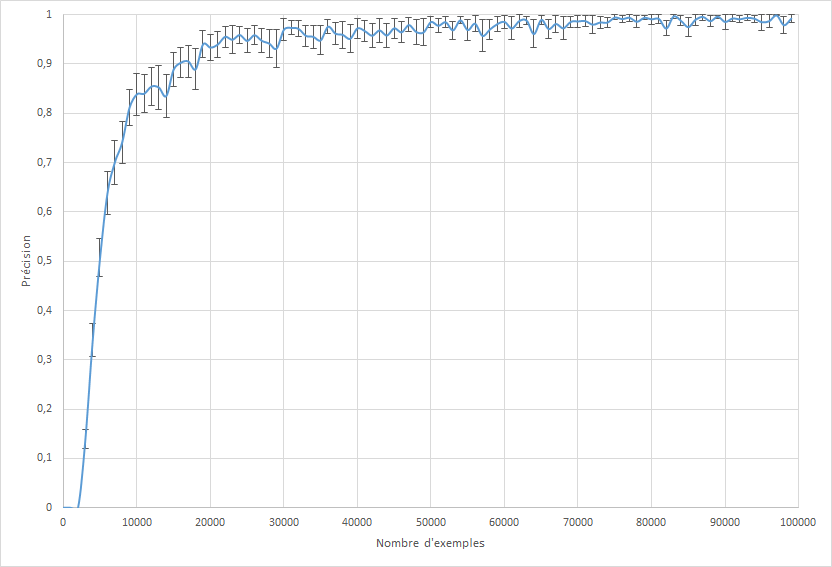
\includegraphics[scale=0.5]{images/chapter6/LSTM_Reber_Sym.png}
\caption{Résultats de l'apprentissage de la grammaire de Reber symétrique pour une cellule LSTM, moyenné sur 100 essais
\ref{lsmt_reber_sym}}
\label{Reber_Sym_LSTM}
\end{center}
\end{figure}

Sur la courbe de la figure \ref{Reber_Sym_LSTM} , il évident qu'une cellule LSTM seule peut apprendre parfaitement une grammaire de Reber symétrique, ce qui n'était pas le cas des réseaux de neurones simples utilisant les algorithmes RTRL et BPTT. En effet ces réseaux ne pouvaient que prédire la moitié des transitions (voir la courbe \ref{Reber_Sym_RTRL_BPTT} ).

Les LSTM peuvent donc apprendre parfaitement une grammaire de Reber au contraire des deux algorithmes appliqués à des réseaux récurrents simples. On peut aussi noter que que l'apprentissage se fait très rapidement et de manière efficace. Les oscillations sont moins conséquentes et surtout il n'y a pas de palier, ce qui montre l'efficacité de l'apprentissage.


Cela montre bien la force des LSTM qui peuvent donc prendre en compte de manière efficace le contexte afin de prédire une suite à ce contexte. C'est dans ce cadre là que nous nous sommes penchés vers la génération de séquence afin de pouvoir vraiment tester les possibilités offertes par celles-ci.
\chapter{Application : génération de texte}

\section{Introduction}

La première application des LSTM à laquelle nous nous sommes intéressés est la génération de texte. Le principe est assez explicite: après apprentissage sur un ensemble de textes, on veut générer un nouvel extrait qui devra répondre aux règles du langage des textes de l'ensemble d'apprentissage.
 

\section{Principe}
On entraine un réseau à prédire la prochaine lettre d'une séquence, puis on lui fait générer des lettres selon cet apprentissage.

\subsection{Architecture du réseau}

Le réseau retenu comporte 2 cellules LSTM dont les états cachés sont de taille 128.
\\ Les caractères du texte sont convertis au format "One Hot Encoded": un caractère est représenté par un vecteur ne contenant que des 0 sauf un 1 à la ligne correspondant à sa nature dans un dictionnaire prédéfinis. La sortie du réseau est un softmax donnant une distribution de probabilité pour la lettre suivante.
\\ Afin de pouvoir fixer le nombre d'état caché indépendamment du format des entrées, il est nécessaire d'ajouter un étage feed forward d'adaptation en sortie du réseau. Ce réseau permettra de passer d'un vecteur de la taille de l'état caché à un vecteur de la taille de la sortie (qui sera aussi la taille de l'entrée dans notre cas).

\subsection{Entrainement}

Les lettres sont présentées en entrée par séquence de longueur fixée. La taille de la séquence correspond à la taille du dépliage que l'on décide de réaliser lors de l'application de l'algorithme BPTT. Cette longueur est donc choisie afin de ne pas produire un dépliage trop volumineux qui demanderait plus de mémoire que ne peut en fournir l'ordinateur.
\\ La figure \ref{LSTM_unfold} montre un tel dépliage sur un exemple simpliste.

\begin{figure}
\begin{center}
% Graphic for TeX using PGF
% Title: C:\Users\marc\Desktop\temp\Diagram1.dia
% Creator: Dia v0.97.2
% CreationDate: Mon Jun 12 22:01:45 2017
% For: marc
% \usepackage{tikz}
% The following commands are not supported in PSTricks at present
% We define them conditionally, so when they are implemented,
% this pgf file will use them.
\ifx\du\undefined
  \newlength{\du}
\fi
\setlength{\du}{15\unitlength}
\begin{tikzpicture}
\pgftransformxscale{1.000000}
\pgftransformyscale{-1.000000}
\definecolor{dialinecolor}{rgb}{0.000000, 0.000000, 0.000000}
\pgfsetstrokecolor{dialinecolor}
\definecolor{dialinecolor}{rgb}{1.000000, 1.000000, 1.000000}
\pgfsetfillcolor{dialinecolor}
\pgfsetlinewidth{0.100000\du}
\pgfsetdash{}{0pt}
\pgfsetdash{}{0pt}
\pgfsetmiterjoin
\definecolor{dialinecolor}{rgb}{1.000000, 1.000000, 1.000000}
\pgfsetfillcolor{dialinecolor}
\fill (16.000000\du,13.000000\du)--(16.000000\du,16.900000\du)--(22.950000\du,16.900000\du)--(22.950000\du,13.000000\du)--cycle;
\definecolor{dialinecolor}{rgb}{0.000000, 0.000000, 0.000000}
\pgfsetstrokecolor{dialinecolor}
\draw (16.000000\du,13.000000\du)--(16.000000\du,16.900000\du)--(22.950000\du,16.900000\du)--(22.950000\du,13.000000\du)--cycle;
\pgfsetlinewidth{0.100000\du}
\pgfsetdash{}{0pt}
\pgfsetdash{}{0pt}
\pgfsetmiterjoin
\definecolor{dialinecolor}{rgb}{1.000000, 1.000000, 1.000000}
\pgfsetfillcolor{dialinecolor}
\fill (15.000000\du,18.000000\du)--(15.000000\du,20.500000\du)--(24.000000\du,20.500000\du)--(24.000000\du,18.000000\du)--cycle;
\definecolor{dialinecolor}{rgb}{0.000000, 0.000000, 0.000000}
\pgfsetstrokecolor{dialinecolor}
\draw (15.000000\du,18.000000\du)--(15.000000\du,20.500000\du)--(24.000000\du,20.500000\du)--(24.000000\du,18.000000\du)--cycle;
\pgfsetlinewidth{0.100000\du}
\pgfsetdash{}{0pt}
\pgfsetdash{}{0pt}
\pgfsetmiterjoin
\definecolor{dialinecolor}{rgb}{1.000000, 1.000000, 1.000000}
\pgfsetfillcolor{dialinecolor}
\fill (15.000000\du,-1.000000\du)--(15.000000\du,1.500000\du)--(24.000000\du,1.500000\du)--(24.000000\du,-1.000000\du)--cycle;
\definecolor{dialinecolor}{rgb}{0.000000, 0.000000, 0.000000}
\pgfsetstrokecolor{dialinecolor}
\draw (15.000000\du,-1.000000\du)--(15.000000\du,1.500000\du)--(24.000000\du,1.500000\du)--(24.000000\du,-1.000000\du)--cycle;
\pgfsetlinewidth{0.100000\du}
\pgfsetdash{}{0pt}
\pgfsetdash{}{0pt}
\pgfsetmiterjoin
\definecolor{dialinecolor}{rgb}{1.000000, 1.000000, 1.000000}
\pgfsetfillcolor{dialinecolor}
\fill (26.000000\du,13.000000\du)--(26.000000\du,16.900000\du)--(32.950000\du,16.900000\du)--(32.950000\du,13.000000\du)--cycle;
\definecolor{dialinecolor}{rgb}{0.000000, 0.000000, 0.000000}
\pgfsetstrokecolor{dialinecolor}
\draw (26.000000\du,13.000000\du)--(26.000000\du,16.900000\du)--(32.950000\du,16.900000\du)--(32.950000\du,13.000000\du)--cycle;
\pgfsetlinewidth{0.100000\du}
\pgfsetdash{}{0pt}
\pgfsetdash{}{0pt}
\pgfsetmiterjoin
\definecolor{dialinecolor}{rgb}{1.000000, 1.000000, 1.000000}
\pgfsetfillcolor{dialinecolor}
\fill (25.000000\du,18.000000\du)--(25.000000\du,20.500000\du)--(34.000000\du,20.500000\du)--(34.000000\du,18.000000\du)--cycle;
\definecolor{dialinecolor}{rgb}{0.000000, 0.000000, 0.000000}
\pgfsetstrokecolor{dialinecolor}
\draw (25.000000\du,18.000000\du)--(25.000000\du,20.500000\du)--(34.000000\du,20.500000\du)--(34.000000\du,18.000000\du)--cycle;
\pgfsetlinewidth{0.100000\du}
\pgfsetdash{}{0pt}
\pgfsetdash{}{0pt}
\pgfsetmiterjoin
\definecolor{dialinecolor}{rgb}{1.000000, 1.000000, 1.000000}
\pgfsetfillcolor{dialinecolor}
\fill (25.000000\du,-1.000000\du)--(25.000000\du,1.500000\du)--(34.000000\du,1.500000\du)--(34.000000\du,-1.000000\du)--cycle;
\definecolor{dialinecolor}{rgb}{0.000000, 0.000000, 0.000000}
\pgfsetstrokecolor{dialinecolor}
\draw (25.000000\du,-1.000000\du)--(25.000000\du,1.500000\du)--(34.000000\du,1.500000\du)--(34.000000\du,-1.000000\du)--cycle;
\pgfsetlinewidth{0.100000\du}
\pgfsetdash{}{0pt}
\pgfsetdash{}{0pt}
\pgfsetmiterjoin
\definecolor{dialinecolor}{rgb}{1.000000, 1.000000, 1.000000}
\pgfsetfillcolor{dialinecolor}
\fill (36.000000\du,13.000000\du)--(36.000000\du,16.900000\du)--(42.950000\du,16.900000\du)--(42.950000\du,13.000000\du)--cycle;
\definecolor{dialinecolor}{rgb}{0.000000, 0.000000, 0.000000}
\pgfsetstrokecolor{dialinecolor}
\draw (36.000000\du,13.000000\du)--(36.000000\du,16.900000\du)--(42.950000\du,16.900000\du)--(42.950000\du,13.000000\du)--cycle;
\pgfsetlinewidth{0.100000\du}
\pgfsetdash{}{0pt}
\pgfsetdash{}{0pt}
\pgfsetmiterjoin
\definecolor{dialinecolor}{rgb}{1.000000, 1.000000, 1.000000}
\pgfsetfillcolor{dialinecolor}
\fill (35.000000\du,18.000000\du)--(35.000000\du,20.500000\du)--(44.000000\du,20.500000\du)--(44.000000\du,18.000000\du)--cycle;
\definecolor{dialinecolor}{rgb}{0.000000, 0.000000, 0.000000}
\pgfsetstrokecolor{dialinecolor}
\draw (35.000000\du,18.000000\du)--(35.000000\du,20.500000\du)--(44.000000\du,20.500000\du)--(44.000000\du,18.000000\du)--cycle;
\pgfsetlinewidth{0.100000\du}
\pgfsetdash{}{0pt}
\pgfsetdash{}{0pt}
\pgfsetmiterjoin
\definecolor{dialinecolor}{rgb}{1.000000, 1.000000, 1.000000}
\pgfsetfillcolor{dialinecolor}
\fill (35.000000\du,-1.000000\du)--(35.000000\du,1.500000\du)--(44.000000\du,1.500000\du)--(44.000000\du,-1.000000\du)--cycle;
\definecolor{dialinecolor}{rgb}{0.000000, 0.000000, 0.000000}
\pgfsetstrokecolor{dialinecolor}
\draw (35.000000\du,-1.000000\du)--(35.000000\du,1.500000\du)--(44.000000\du,1.500000\du)--(44.000000\du,-1.000000\du)--cycle;
\pgfsetlinewidth{0.100000\du}
\pgfsetdash{}{0pt}
\pgfsetdash{}{0pt}
\pgfsetmiterjoin
\definecolor{dialinecolor}{rgb}{1.000000, 1.000000, 1.000000}
\pgfsetfillcolor{dialinecolor}
\fill (46.000000\du,13.000000\du)--(46.000000\du,16.900000\du)--(52.950000\du,16.900000\du)--(52.950000\du,13.000000\du)--cycle;
\definecolor{dialinecolor}{rgb}{0.000000, 0.000000, 0.000000}
\pgfsetstrokecolor{dialinecolor}
\draw (46.000000\du,13.000000\du)--(46.000000\du,16.900000\du)--(52.950000\du,16.900000\du)--(52.950000\du,13.000000\du)--cycle;
\pgfsetlinewidth{0.100000\du}
\pgfsetdash{}{0pt}
\pgfsetdash{}{0pt}
\pgfsetmiterjoin
\definecolor{dialinecolor}{rgb}{1.000000, 1.000000, 1.000000}
\pgfsetfillcolor{dialinecolor}
\fill (45.000000\du,18.000000\du)--(45.000000\du,20.500000\du)--(53.950000\du,20.500000\du)--(53.950000\du,18.000000\du)--cycle;
\definecolor{dialinecolor}{rgb}{0.000000, 0.000000, 0.000000}
\pgfsetstrokecolor{dialinecolor}
\draw (45.000000\du,18.000000\du)--(45.000000\du,20.500000\du)--(53.950000\du,20.500000\du)--(53.950000\du,18.000000\du)--cycle;
\pgfsetlinewidth{0.100000\du}
\pgfsetdash{}{0pt}
\pgfsetdash{}{0pt}
\pgfsetmiterjoin
\definecolor{dialinecolor}{rgb}{1.000000, 1.000000, 1.000000}
\pgfsetfillcolor{dialinecolor}
\fill (45.000000\du,-1.000000\du)--(45.000000\du,1.500000\du)--(54.000000\du,1.500000\du)--(54.000000\du,-1.000000\du)--cycle;
\definecolor{dialinecolor}{rgb}{0.000000, 0.000000, 0.000000}
\pgfsetstrokecolor{dialinecolor}
\draw (45.000000\du,-1.000000\du)--(45.000000\du,1.500000\du)--(54.000000\du,1.500000\du)--(54.000000\du,-1.000000\du)--cycle;
% setfont left to latex
\definecolor{dialinecolor}{rgb}{0.000000, 0.000000, 1.000000}
\pgfsetstrokecolor{dialinecolor}
\node at (19.500000\du,0.890000\du){prédiction : \ensuremath{[} 0 0.5 0.5 \ensuremath{]}};
\pgfsetlinewidth{0.100000\du}
\pgfsetdash{}{0pt}
\pgfsetdash{}{0pt}
\pgfsetbuttcap
{
\definecolor{dialinecolor}{rgb}{0.000000, 0.000000, 0.000000}
\pgfsetfillcolor{dialinecolor}
% was here!!!
\pgfsetarrowsend{stealth}
\definecolor{dialinecolor}{rgb}{0.000000, 0.000000, 0.000000}
\pgfsetstrokecolor{dialinecolor}
\draw (22.950000\du,14.950000\du)--(26.000000\du,14.950000\du);
}
\pgfsetlinewidth{0.100000\du}
\pgfsetdash{}{0pt}
\pgfsetdash{}{0pt}
\pgfsetbuttcap
{
\definecolor{dialinecolor}{rgb}{0.000000, 0.000000, 0.000000}
\pgfsetfillcolor{dialinecolor}
% was here!!!
\pgfsetarrowsend{stealth}
\definecolor{dialinecolor}{rgb}{0.000000, 0.000000, 0.000000}
\pgfsetstrokecolor{dialinecolor}
\draw (32.950000\du,14.950000\du)--(36.000000\du,14.950000\du);
}
\pgfsetlinewidth{0.100000\du}
\pgfsetdash{}{0pt}
\pgfsetdash{}{0pt}
\pgfsetbuttcap
{
\definecolor{dialinecolor}{rgb}{0.000000, 0.000000, 0.000000}
\pgfsetfillcolor{dialinecolor}
% was here!!!
\pgfsetarrowsend{stealth}
\definecolor{dialinecolor}{rgb}{0.000000, 0.000000, 0.000000}
\pgfsetstrokecolor{dialinecolor}
\draw (42.950000\du,14.950000\du)--(46.000000\du,14.950000\du);
}
% setfont left to latex
\definecolor{dialinecolor}{rgb}{0.000000, 0.000000, 0.000000}
\pgfsetstrokecolor{dialinecolor}
\node at (19.475000\du,15.194094\du){LSTM1 (t)};
\pgfsetlinewidth{0.100000\du}
\pgfsetdash{}{0pt}
\pgfsetdash{}{0pt}
\pgfsetbuttcap
{
\definecolor{dialinecolor}{rgb}{0.000000, 0.000000, 0.000000}
\pgfsetfillcolor{dialinecolor}
% was here!!!
\pgfsetarrowsend{stealth}
\definecolor{dialinecolor}{rgb}{0.000000, 0.000000, 0.000000}
\pgfsetstrokecolor{dialinecolor}
\draw (19.500000\du,18.000000\du)--(19.475000\du,16.900000\du);
}
\pgfsetlinewidth{0.100000\du}
\pgfsetdash{}{0pt}
\pgfsetdash{}{0pt}
\pgfsetbuttcap
{
\definecolor{dialinecolor}{rgb}{0.000000, 0.000000, 0.000000}
\pgfsetfillcolor{dialinecolor}
% was here!!!
\pgfsetarrowsend{stealth}
\definecolor{dialinecolor}{rgb}{0.000000, 0.000000, 0.000000}
\pgfsetstrokecolor{dialinecolor}
\draw (49.475000\du,18.000000\du)--(49.475000\du,16.900000\du);
}
\pgfsetlinewidth{0.100000\du}
\pgfsetdash{}{0pt}
\pgfsetdash{}{0pt}
\pgfsetbuttcap
{
\definecolor{dialinecolor}{rgb}{0.000000, 0.000000, 0.000000}
\pgfsetfillcolor{dialinecolor}
% was here!!!
\pgfsetarrowsend{stealth}
\definecolor{dialinecolor}{rgb}{0.000000, 0.000000, 0.000000}
\pgfsetstrokecolor{dialinecolor}
\draw (39.500000\du,18.000000\du)--(39.475000\du,16.900000\du);
}
\pgfsetlinewidth{0.100000\du}
\pgfsetdash{}{0pt}
\pgfsetdash{}{0pt}
\pgfsetbuttcap
{
\definecolor{dialinecolor}{rgb}{0.000000, 0.000000, 0.000000}
\pgfsetfillcolor{dialinecolor}
% was here!!!
\pgfsetarrowsend{stealth}
\definecolor{dialinecolor}{rgb}{0.000000, 0.000000, 0.000000}
\pgfsetstrokecolor{dialinecolor}
\draw (29.500000\du,18.000000\du)--(29.475000\du,16.900000\du);
}
% setfont left to latex
\definecolor{dialinecolor}{rgb}{0.000000, 0.000000, 0.000000}
\pgfsetstrokecolor{dialinecolor}
\node at (19.500000\du,0.117500\du){séquence (t+1) : \ensuremath{[} 1 0 0 \ensuremath{]}};
% setfont left to latex
\definecolor{dialinecolor}{rgb}{0.000000, 0.000000, 0.000000}
\pgfsetstrokecolor{dialinecolor}
\node at (19.500000\du,19.494094\du){séquence (t) : \ensuremath{[} 0 1 0 \ensuremath{]}};
% setfont left to latex
\definecolor{dialinecolor}{rgb}{0.000000, 0.000000, 0.000000}
\pgfsetstrokecolor{dialinecolor}
\node at (29.475000\du,15.194094\du){LSTM1 (t+1)};
% setfont left to latex
\definecolor{dialinecolor}{rgb}{0.000000, 0.000000, 0.000000}
\pgfsetstrokecolor{dialinecolor}
\node[anchor=west] at (29.500000\du,0.250000\du){};
% setfont left to latex
\definecolor{dialinecolor}{rgb}{0.000000, 0.000000, 0.000000}
\pgfsetstrokecolor{dialinecolor}
\node at (29.500000\du,0.117500\du){séquence (t+2) : \ensuremath{[} 0 0 1 \ensuremath{]}};
% setfont left to latex
\definecolor{dialinecolor}{rgb}{0.000000, 0.000000, 1.000000}
\pgfsetstrokecolor{dialinecolor}
\node at (29.500000\du,0.890000\du){prédiction : \ensuremath{[} 0.3 0.7 0 \ensuremath{]}};
% setfont left to latex
\definecolor{dialinecolor}{rgb}{0.000000, 0.000000, 0.000000}
\pgfsetstrokecolor{dialinecolor}
\node at (29.500000\du,19.494094\du){séquence (t+1) : \ensuremath{[} 1 0 0 \ensuremath{]}};
% setfont left to latex
\definecolor{dialinecolor}{rgb}{0.000000, 0.000000, 0.000000}
\pgfsetstrokecolor{dialinecolor}
\node at (39.500000\du,19.494094\du){séquence (t+2) : \ensuremath{[} 0 0 1 \ensuremath{]}};
% setfont left to latex
\definecolor{dialinecolor}{rgb}{0.000000, 0.000000, 0.000000}
\pgfsetstrokecolor{dialinecolor}
\node at (39.475000\du,15.194094\du){LSTM1 (t+2)};
% setfont left to latex
\definecolor{dialinecolor}{rgb}{0.000000, 0.000000, 0.000000}
\pgfsetstrokecolor{dialinecolor}
\node at (49.475000\du,15.194094\du){LSTM1 (t+3)};
% setfont left to latex
\definecolor{dialinecolor}{rgb}{0.000000, 0.000000, 1.000000}
\pgfsetstrokecolor{dialinecolor}
\node at (39.500000\du,0.890000\du){prédiction : \ensuremath{[} 0.3 0.2 0.5 \ensuremath{]}};
% setfont left to latex
\definecolor{dialinecolor}{rgb}{0.000000, 0.000000, 1.000000}
\pgfsetstrokecolor{dialinecolor}
\node at (49.500000\du,0.890000\du){prédiction : \ensuremath{[} 0.1 0.2 0.7 \ensuremath{]}};
% setfont left to latex
\definecolor{dialinecolor}{rgb}{0.000000, 0.000000, 0.000000}
\pgfsetstrokecolor{dialinecolor}
\node at (49.475000\du,19.494094\du){séquence (t+3) : \ensuremath{[} 1 0 0 \ensuremath{]}};
% setfont left to latex
\definecolor{dialinecolor}{rgb}{0.000000, 0.000000, 0.000000}
\pgfsetstrokecolor{dialinecolor}
\node at (39.500000\du,0.117500\du){séquence (t+3) : \ensuremath{[} 0 0 1 \ensuremath{]}};
% setfont left to latex
\definecolor{dialinecolor}{rgb}{0.000000, 0.000000, 0.000000}
\pgfsetstrokecolor{dialinecolor}
\node at (49.500000\du,0.117500\du){séquence (t+4) : \ensuremath{[} 0 0 1 \ensuremath{]}};
\pgfsetlinewidth{0.100000\du}
\pgfsetdash{}{0pt}
\pgfsetdash{}{0pt}
\pgfsetmiterjoin
\definecolor{dialinecolor}{rgb}{1.000000, 1.000000, 1.000000}
\pgfsetfillcolor{dialinecolor}
\fill (16.000000\du,8.000000\du)--(16.000000\du,11.900000\du)--(22.950000\du,11.900000\du)--(22.950000\du,8.000000\du)--cycle;
\definecolor{dialinecolor}{rgb}{0.000000, 0.000000, 0.000000}
\pgfsetstrokecolor{dialinecolor}
\draw (16.000000\du,8.000000\du)--(16.000000\du,11.900000\du)--(22.950000\du,11.900000\du)--(22.950000\du,8.000000\du)--cycle;
\pgfsetlinewidth{0.100000\du}
\pgfsetdash{}{0pt}
\pgfsetdash{}{0pt}
\pgfsetmiterjoin
\definecolor{dialinecolor}{rgb}{1.000000, 1.000000, 1.000000}
\pgfsetfillcolor{dialinecolor}
\fill (26.000000\du,8.000000\du)--(26.000000\du,11.900000\du)--(32.950000\du,11.900000\du)--(32.950000\du,8.000000\du)--cycle;
\definecolor{dialinecolor}{rgb}{0.000000, 0.000000, 0.000000}
\pgfsetstrokecolor{dialinecolor}
\draw (26.000000\du,8.000000\du)--(26.000000\du,11.900000\du)--(32.950000\du,11.900000\du)--(32.950000\du,8.000000\du)--cycle;
\pgfsetlinewidth{0.100000\du}
\pgfsetdash{}{0pt}
\pgfsetdash{}{0pt}
\pgfsetmiterjoin
\definecolor{dialinecolor}{rgb}{1.000000, 1.000000, 1.000000}
\pgfsetfillcolor{dialinecolor}
\fill (36.000000\du,8.000000\du)--(36.000000\du,11.900000\du)--(42.950000\du,11.900000\du)--(42.950000\du,8.000000\du)--cycle;
\definecolor{dialinecolor}{rgb}{0.000000, 0.000000, 0.000000}
\pgfsetstrokecolor{dialinecolor}
\draw (36.000000\du,8.000000\du)--(36.000000\du,11.900000\du)--(42.950000\du,11.900000\du)--(42.950000\du,8.000000\du)--cycle;
\pgfsetlinewidth{0.100000\du}
\pgfsetdash{}{0pt}
\pgfsetdash{}{0pt}
\pgfsetmiterjoin
\definecolor{dialinecolor}{rgb}{1.000000, 1.000000, 1.000000}
\pgfsetfillcolor{dialinecolor}
\fill (46.000000\du,8.000000\du)--(46.000000\du,11.900000\du)--(52.950000\du,11.900000\du)--(52.950000\du,8.000000\du)--cycle;
\definecolor{dialinecolor}{rgb}{0.000000, 0.000000, 0.000000}
\pgfsetstrokecolor{dialinecolor}
\draw (46.000000\du,8.000000\du)--(46.000000\du,11.900000\du)--(52.950000\du,11.900000\du)--(52.950000\du,8.000000\du)--cycle;
\pgfsetlinewidth{0.100000\du}
\pgfsetdash{}{0pt}
\pgfsetdash{}{0pt}
\pgfsetbuttcap
{
\definecolor{dialinecolor}{rgb}{0.000000, 0.000000, 0.000000}
\pgfsetfillcolor{dialinecolor}
% was here!!!
\pgfsetarrowsend{stealth}
\definecolor{dialinecolor}{rgb}{0.000000, 0.000000, 0.000000}
\pgfsetstrokecolor{dialinecolor}
\draw (22.950000\du,9.950000\du)--(26.000000\du,9.950000\du);
}
\pgfsetlinewidth{0.100000\du}
\pgfsetdash{}{0pt}
\pgfsetdash{}{0pt}
\pgfsetbuttcap
{
\definecolor{dialinecolor}{rgb}{0.000000, 0.000000, 0.000000}
\pgfsetfillcolor{dialinecolor}
% was here!!!
\pgfsetarrowsend{stealth}
\definecolor{dialinecolor}{rgb}{0.000000, 0.000000, 0.000000}
\pgfsetstrokecolor{dialinecolor}
\draw (32.950000\du,9.950000\du)--(36.000000\du,9.950000\du);
}
\pgfsetlinewidth{0.100000\du}
\pgfsetdash{}{0pt}
\pgfsetdash{}{0pt}
\pgfsetbuttcap
{
\definecolor{dialinecolor}{rgb}{0.000000, 0.000000, 0.000000}
\pgfsetfillcolor{dialinecolor}
% was here!!!
\pgfsetarrowsend{stealth}
\definecolor{dialinecolor}{rgb}{0.000000, 0.000000, 0.000000}
\pgfsetstrokecolor{dialinecolor}
\draw (42.950000\du,9.950000\du)--(46.000000\du,9.950000\du);
}
% setfont left to latex
\definecolor{dialinecolor}{rgb}{0.000000, 0.000000, 0.000000}
\pgfsetstrokecolor{dialinecolor}
\node at (19.475000\du,10.194094\du){LSTM2 (t)};
\pgfsetlinewidth{0.100000\du}
\pgfsetdash{}{0pt}
\pgfsetdash{}{0pt}
\pgfsetbuttcap
{
\definecolor{dialinecolor}{rgb}{0.000000, 0.000000, 0.000000}
\pgfsetfillcolor{dialinecolor}
% was here!!!
\pgfsetarrowsend{stealth}
\definecolor{dialinecolor}{rgb}{0.000000, 0.000000, 0.000000}
\pgfsetstrokecolor{dialinecolor}
\draw (19.475000\du,13.000000\du)--(19.475000\du,11.900000\du);
}
\pgfsetlinewidth{0.100000\du}
\pgfsetdash{}{0pt}
\pgfsetdash{}{0pt}
\pgfsetbuttcap
{
\definecolor{dialinecolor}{rgb}{0.000000, 0.000000, 0.000000}
\pgfsetfillcolor{dialinecolor}
% was here!!!
\pgfsetarrowsend{stealth}
\definecolor{dialinecolor}{rgb}{0.000000, 0.000000, 0.000000}
\pgfsetstrokecolor{dialinecolor}
\draw (49.475000\du,13.000000\du)--(49.475000\du,11.900000\du);
}
\pgfsetlinewidth{0.100000\du}
\pgfsetdash{}{0pt}
\pgfsetdash{}{0pt}
\pgfsetbuttcap
{
\definecolor{dialinecolor}{rgb}{0.000000, 0.000000, 0.000000}
\pgfsetfillcolor{dialinecolor}
% was here!!!
\pgfsetarrowsend{stealth}
\definecolor{dialinecolor}{rgb}{0.000000, 0.000000, 0.000000}
\pgfsetstrokecolor{dialinecolor}
\draw (39.475000\du,13.000000\du)--(39.475000\du,11.900000\du);
}
\pgfsetlinewidth{0.100000\du}
\pgfsetdash{}{0pt}
\pgfsetdash{}{0pt}
\pgfsetbuttcap
{
\definecolor{dialinecolor}{rgb}{0.000000, 0.000000, 0.000000}
\pgfsetfillcolor{dialinecolor}
% was here!!!
\pgfsetarrowsend{stealth}
\definecolor{dialinecolor}{rgb}{0.000000, 0.000000, 0.000000}
\pgfsetstrokecolor{dialinecolor}
\draw (29.475000\du,13.000000\du)--(29.475000\du,11.900000\du);
}
% setfont left to latex
\definecolor{dialinecolor}{rgb}{0.000000, 0.000000, 0.000000}
\pgfsetstrokecolor{dialinecolor}
\node at (29.475000\du,10.194094\du){LSTM2 (t+1)};
% setfont left to latex
\definecolor{dialinecolor}{rgb}{0.000000, 0.000000, 0.000000}
\pgfsetstrokecolor{dialinecolor}
\node at (39.475000\du,10.194094\du){LSTM2 (t+2)};
% setfont left to latex
\definecolor{dialinecolor}{rgb}{0.000000, 0.000000, 0.000000}
\pgfsetstrokecolor{dialinecolor}
\node at (49.475000\du,10.194094\du){LSTM2 (t+3)};
\pgfsetlinewidth{0.100000\du}
\pgfsetdash{}{0pt}
\pgfsetdash{}{0pt}
\pgfsetmiterjoin
\definecolor{dialinecolor}{rgb}{1.000000, 1.000000, 1.000000}
\pgfsetfillcolor{dialinecolor}
\fill (16.000000\du,3.000000\du)--(16.000000\du,6.900000\du)--(22.950000\du,6.900000\du)--(22.950000\du,3.000000\du)--cycle;
\definecolor{dialinecolor}{rgb}{0.000000, 0.000000, 0.000000}
\pgfsetstrokecolor{dialinecolor}
\draw (16.000000\du,3.000000\du)--(16.000000\du,6.900000\du)--(22.950000\du,6.900000\du)--(22.950000\du,3.000000\du)--cycle;
\pgfsetlinewidth{0.100000\du}
\pgfsetdash{}{0pt}
\pgfsetdash{}{0pt}
\pgfsetmiterjoin
\definecolor{dialinecolor}{rgb}{1.000000, 1.000000, 1.000000}
\pgfsetfillcolor{dialinecolor}
\fill (26.000000\du,3.000000\du)--(26.000000\du,6.900000\du)--(32.950000\du,6.900000\du)--(32.950000\du,3.000000\du)--cycle;
\definecolor{dialinecolor}{rgb}{0.000000, 0.000000, 0.000000}
\pgfsetstrokecolor{dialinecolor}
\draw (26.000000\du,3.000000\du)--(26.000000\du,6.900000\du)--(32.950000\du,6.900000\du)--(32.950000\du,3.000000\du)--cycle;
\pgfsetlinewidth{0.100000\du}
\pgfsetdash{}{0pt}
\pgfsetdash{}{0pt}
\pgfsetmiterjoin
\definecolor{dialinecolor}{rgb}{1.000000, 1.000000, 1.000000}
\pgfsetfillcolor{dialinecolor}
\fill (36.000000\du,3.000000\du)--(36.000000\du,6.900000\du)--(42.950000\du,6.900000\du)--(42.950000\du,3.000000\du)--cycle;
\definecolor{dialinecolor}{rgb}{0.000000, 0.000000, 0.000000}
\pgfsetstrokecolor{dialinecolor}
\draw (36.000000\du,3.000000\du)--(36.000000\du,6.900000\du)--(42.950000\du,6.900000\du)--(42.950000\du,3.000000\du)--cycle;
\pgfsetlinewidth{0.100000\du}
\pgfsetdash{}{0pt}
\pgfsetdash{}{0pt}
\pgfsetmiterjoin
\definecolor{dialinecolor}{rgb}{1.000000, 1.000000, 1.000000}
\pgfsetfillcolor{dialinecolor}
\fill (46.000000\du,3.000000\du)--(46.000000\du,6.900000\du)--(52.950000\du,6.900000\du)--(52.950000\du,3.000000\du)--cycle;
\definecolor{dialinecolor}{rgb}{0.000000, 0.000000, 0.000000}
\pgfsetstrokecolor{dialinecolor}
\draw (46.000000\du,3.000000\du)--(46.000000\du,6.900000\du)--(52.950000\du,6.900000\du)--(52.950000\du,3.000000\du)--cycle;
% setfont left to latex
\definecolor{dialinecolor}{rgb}{0.000000, 0.000000, 0.000000}
\pgfsetstrokecolor{dialinecolor}
\node at (19.475000\du,5.194094\du){réseau d'adaptation};
\pgfsetlinewidth{0.100000\du}
\pgfsetdash{}{0pt}
\pgfsetdash{}{0pt}
\pgfsetbuttcap
{
\definecolor{dialinecolor}{rgb}{0.000000, 0.000000, 0.000000}
\pgfsetfillcolor{dialinecolor}
% was here!!!
\pgfsetarrowsend{stealth}
\definecolor{dialinecolor}{rgb}{0.000000, 0.000000, 0.000000}
\pgfsetstrokecolor{dialinecolor}
\draw (19.475000\du,8.000000\du)--(19.475000\du,6.900000\du);
}
\pgfsetlinewidth{0.100000\du}
\pgfsetdash{}{0pt}
\pgfsetdash{}{0pt}
\pgfsetbuttcap
{
\definecolor{dialinecolor}{rgb}{0.000000, 0.000000, 0.000000}
\pgfsetfillcolor{dialinecolor}
% was here!!!
\pgfsetarrowsend{stealth}
\definecolor{dialinecolor}{rgb}{0.000000, 0.000000, 0.000000}
\pgfsetstrokecolor{dialinecolor}
\draw (49.475000\du,8.000000\du)--(49.475000\du,6.900000\du);
}
\pgfsetlinewidth{0.100000\du}
\pgfsetdash{}{0pt}
\pgfsetdash{}{0pt}
\pgfsetbuttcap
{
\definecolor{dialinecolor}{rgb}{0.000000, 0.000000, 0.000000}
\pgfsetfillcolor{dialinecolor}
% was here!!!
\pgfsetarrowsend{stealth}
\definecolor{dialinecolor}{rgb}{0.000000, 0.000000, 0.000000}
\pgfsetstrokecolor{dialinecolor}
\draw (39.475000\du,8.000000\du)--(39.475000\du,6.900000\du);
}
\pgfsetlinewidth{0.100000\du}
\pgfsetdash{}{0pt}
\pgfsetdash{}{0pt}
\pgfsetbuttcap
{
\definecolor{dialinecolor}{rgb}{0.000000, 0.000000, 0.000000}
\pgfsetfillcolor{dialinecolor}
% was here!!!
\pgfsetarrowsend{stealth}
\definecolor{dialinecolor}{rgb}{0.000000, 0.000000, 0.000000}
\pgfsetstrokecolor{dialinecolor}
\draw (29.475000\du,8.000000\du)--(29.475000\du,6.900000\du);
}
% setfont left to latex
\definecolor{dialinecolor}{rgb}{0.000000, 0.000000, 0.000000}
\pgfsetstrokecolor{dialinecolor}
\node at (29.475000\du,5.194094\du){réseau d'adaptation};
% setfont left to latex
\definecolor{dialinecolor}{rgb}{0.000000, 0.000000, 0.000000}
\pgfsetstrokecolor{dialinecolor}
\node at (39.475000\du,5.194094\du){réseau d'adaptation};
% setfont left to latex
\definecolor{dialinecolor}{rgb}{0.000000, 0.000000, 0.000000}
\pgfsetstrokecolor{dialinecolor}
\node at (49.475000\du,5.194094\du){réseau d'adaptation};
\pgfsetlinewidth{0.100000\du}
\pgfsetdash{}{0pt}
\pgfsetdash{}{0pt}
\pgfsetbuttcap
{
\definecolor{dialinecolor}{rgb}{0.000000, 0.000000, 0.000000}
\pgfsetfillcolor{dialinecolor}
% was here!!!
\pgfsetarrowsend{stealth}
\definecolor{dialinecolor}{rgb}{0.000000, 0.000000, 0.000000}
\pgfsetstrokecolor{dialinecolor}
\draw (19.475000\du,3.000000\du)--(19.500000\du,1.500000\du);
}
\pgfsetlinewidth{0.100000\du}
\pgfsetdash{}{0pt}
\pgfsetdash{}{0pt}
\pgfsetbuttcap
{
\definecolor{dialinecolor}{rgb}{0.000000, 0.000000, 0.000000}
\pgfsetfillcolor{dialinecolor}
% was here!!!
\pgfsetarrowsend{stealth}
\definecolor{dialinecolor}{rgb}{0.000000, 0.000000, 0.000000}
\pgfsetstrokecolor{dialinecolor}
\draw (29.475000\du,3.000000\du)--(29.500000\du,1.500000\du);
}
\pgfsetlinewidth{0.100000\du}
\pgfsetdash{}{0pt}
\pgfsetdash{}{0pt}
\pgfsetbuttcap
{
\definecolor{dialinecolor}{rgb}{0.000000, 0.000000, 0.000000}
\pgfsetfillcolor{dialinecolor}
% was here!!!
\pgfsetarrowsend{stealth}
\definecolor{dialinecolor}{rgb}{0.000000, 0.000000, 0.000000}
\pgfsetstrokecolor{dialinecolor}
\draw (39.475000\du,3.000000\du)--(39.500000\du,1.500000\du);
}
\pgfsetlinewidth{0.100000\du}
\pgfsetdash{}{0pt}
\pgfsetdash{}{0pt}
\pgfsetbuttcap
{
\definecolor{dialinecolor}{rgb}{0.000000, 0.000000, 0.000000}
\pgfsetfillcolor{dialinecolor}
% was here!!!
\pgfsetarrowsend{stealth}
\definecolor{dialinecolor}{rgb}{0.000000, 0.000000, 0.000000}
\pgfsetstrokecolor{dialinecolor}
\draw (49.475000\du,3.000000\du)--(49.488181\du,1.550140\du);
}
\end{tikzpicture}

\caption{Exemple de dépliage de longueur 4 pour l'apprentissage de séquence}
\label{LSTM_unfold}
\end{center}
\end{figure}

Dans notre implémentation l'apprentissage est accéléré en traitant plusieurs séquences en parallèle. On met alors non plus un vecteur représentant un caractère en entrée mais une matrice représentant les caractères au temps $t$ de chacune des séquences dont on parallélise l'apprentissage. La diminution du temps de calcul provient de l'optimisation des calculs matriciels de Numpy.

\subsection{Génération}


Pour générer un extrait de texte, on donne en entrée du réseau au temps $t+1$ une lettre obtenue par tirage sur la distribution probabiliste obtenue en sortie du dernier étage au temps $t$.
La première est choisie arbitrairement.
\\La figure \ref{LSTM_generate} développe un exemple simpliste de génération.

\begin{figure}
\begin{center}
% Graphic for TeX using PGF
% Title: C:\Users\marc\Desktop\temp\Diagram1.dia
% Creator: Dia v0.97.2
% CreationDate: Mon Jun 12 22:22:20 2017
% For: marc
% \usepackage{tikz}
% The following commands are not supported in PSTricks at present
% We define them conditionally, so when they are implemented,
% this pgf file will use them.
\ifx\du\undefined
  \newlength{\du}
\fi
\setlength{\du}{15\unitlength}
\begin{tikzpicture}
\pgftransformxscale{1.000000}
\pgftransformyscale{-1.000000}
\definecolor{dialinecolor}{rgb}{0.000000, 0.000000, 0.000000}
\pgfsetstrokecolor{dialinecolor}
\definecolor{dialinecolor}{rgb}{1.000000, 1.000000, 1.000000}
\pgfsetfillcolor{dialinecolor}
\pgfsetlinewidth{0.100000\du}
\pgfsetdash{}{0pt}
\pgfsetdash{}{0pt}
\pgfsetmiterjoin
\definecolor{dialinecolor}{rgb}{1.000000, 1.000000, 1.000000}
\pgfsetfillcolor{dialinecolor}
\fill (4.000000\du,13.000000\du)--(4.000000\du,16.900000\du)--(10.950000\du,16.900000\du)--(10.950000\du,13.000000\du)--cycle;
\definecolor{dialinecolor}{rgb}{0.000000, 0.000000, 0.000000}
\pgfsetstrokecolor{dialinecolor}
\draw (4.000000\du,13.000000\du)--(4.000000\du,16.900000\du)--(10.950000\du,16.900000\du)--(10.950000\du,13.000000\du)--cycle;
\pgfsetlinewidth{0.100000\du}
\pgfsetdash{}{0pt}
\pgfsetdash{}{0pt}
\pgfsetmiterjoin
\definecolor{dialinecolor}{rgb}{1.000000, 1.000000, 1.000000}
\pgfsetfillcolor{dialinecolor}
\fill (3.000000\du,18.000000\du)--(3.000000\du,20.000000\du)--(12.000000\du,20.000000\du)--(12.000000\du,18.000000\du)--cycle;
\definecolor{dialinecolor}{rgb}{0.000000, 0.000000, 0.000000}
\pgfsetstrokecolor{dialinecolor}
\draw (3.000000\du,18.000000\du)--(3.000000\du,20.000000\du)--(12.000000\du,20.000000\du)--(12.000000\du,18.000000\du)--cycle;
\pgfsetlinewidth{0.100000\du}
\pgfsetdash{}{0pt}
\pgfsetdash{}{0pt}
\pgfsetmiterjoin
\definecolor{dialinecolor}{rgb}{1.000000, 1.000000, 1.000000}
\pgfsetfillcolor{dialinecolor}
\fill (3.000000\du,-1.000000\du)--(3.000000\du,1.500000\du)--(12.000000\du,1.500000\du)--(12.000000\du,-1.000000\du)--cycle;
\definecolor{dialinecolor}{rgb}{0.000000, 0.000000, 0.000000}
\pgfsetstrokecolor{dialinecolor}
\draw (3.000000\du,-1.000000\du)--(3.000000\du,1.500000\du)--(12.000000\du,1.500000\du)--(12.000000\du,-1.000000\du)--cycle;
\pgfsetlinewidth{0.100000\du}
\pgfsetdash{}{0pt}
\pgfsetdash{}{0pt}
\pgfsetmiterjoin
\definecolor{dialinecolor}{rgb}{1.000000, 1.000000, 1.000000}
\pgfsetfillcolor{dialinecolor}
\fill (23.000000\du,13.000000\du)--(23.000000\du,16.900000\du)--(29.950000\du,16.900000\du)--(29.950000\du,13.000000\du)--cycle;
\definecolor{dialinecolor}{rgb}{0.000000, 0.000000, 0.000000}
\pgfsetstrokecolor{dialinecolor}
\draw (23.000000\du,13.000000\du)--(23.000000\du,16.900000\du)--(29.950000\du,16.900000\du)--(29.950000\du,13.000000\du)--cycle;
\pgfsetlinewidth{0.100000\du}
\pgfsetdash{}{0pt}
\pgfsetdash{}{0pt}
\pgfsetmiterjoin
\definecolor{dialinecolor}{rgb}{1.000000, 1.000000, 1.000000}
\pgfsetfillcolor{dialinecolor}
\fill (22.000000\du,18.000000\du)--(22.000000\du,20.000000\du)--(31.000000\du,20.000000\du)--(31.000000\du,18.000000\du)--cycle;
\definecolor{dialinecolor}{rgb}{0.000000, 0.000000, 0.000000}
\pgfsetstrokecolor{dialinecolor}
\draw (22.000000\du,18.000000\du)--(22.000000\du,20.000000\du)--(31.000000\du,20.000000\du)--(31.000000\du,18.000000\du)--cycle;
\pgfsetlinewidth{0.100000\du}
\pgfsetdash{}{0pt}
\pgfsetdash{}{0pt}
\pgfsetmiterjoin
\definecolor{dialinecolor}{rgb}{1.000000, 1.000000, 1.000000}
\pgfsetfillcolor{dialinecolor}
\fill (22.000000\du,-1.000000\du)--(22.000000\du,1.500000\du)--(31.000000\du,1.500000\du)--(31.000000\du,-1.000000\du)--cycle;
\definecolor{dialinecolor}{rgb}{0.000000, 0.000000, 0.000000}
\pgfsetstrokecolor{dialinecolor}
\draw (22.000000\du,-1.000000\du)--(22.000000\du,1.500000\du)--(31.000000\du,1.500000\du)--(31.000000\du,-1.000000\du)--cycle;
\pgfsetlinewidth{0.100000\du}
\pgfsetdash{}{0pt}
\pgfsetdash{}{0pt}
\pgfsetmiterjoin
\definecolor{dialinecolor}{rgb}{1.000000, 1.000000, 1.000000}
\pgfsetfillcolor{dialinecolor}
\fill (42.000000\du,13.000000\du)--(42.000000\du,16.900000\du)--(48.950000\du,16.900000\du)--(48.950000\du,13.000000\du)--cycle;
\definecolor{dialinecolor}{rgb}{0.000000, 0.000000, 0.000000}
\pgfsetstrokecolor{dialinecolor}
\draw (42.000000\du,13.000000\du)--(42.000000\du,16.900000\du)--(48.950000\du,16.900000\du)--(48.950000\du,13.000000\du)--cycle;
\pgfsetlinewidth{0.100000\du}
\pgfsetdash{}{0pt}
\pgfsetdash{}{0pt}
\pgfsetmiterjoin
\definecolor{dialinecolor}{rgb}{1.000000, 1.000000, 1.000000}
\pgfsetfillcolor{dialinecolor}
\fill (41.000000\du,18.000000\du)--(41.000000\du,20.000000\du)--(50.000000\du,20.000000\du)--(50.000000\du,18.000000\du)--cycle;
\definecolor{dialinecolor}{rgb}{0.000000, 0.000000, 0.000000}
\pgfsetstrokecolor{dialinecolor}
\draw (41.000000\du,18.000000\du)--(41.000000\du,20.000000\du)--(50.000000\du,20.000000\du)--(50.000000\du,18.000000\du)--cycle;
\pgfsetlinewidth{0.100000\du}
\pgfsetdash{}{0pt}
\pgfsetdash{}{0pt}
\pgfsetmiterjoin
\definecolor{dialinecolor}{rgb}{1.000000, 1.000000, 1.000000}
\pgfsetfillcolor{dialinecolor}
\fill (41.000000\du,-1.000000\du)--(41.000000\du,1.500000\du)--(50.000000\du,1.500000\du)--(50.000000\du,-1.000000\du)--cycle;
\definecolor{dialinecolor}{rgb}{0.000000, 0.000000, 0.000000}
\pgfsetstrokecolor{dialinecolor}
\draw (41.000000\du,-1.000000\du)--(41.000000\du,1.500000\du)--(50.000000\du,1.500000\du)--(50.000000\du,-1.000000\du)--cycle;
% setfont left to latex
\definecolor{dialinecolor}{rgb}{0.000000, 0.000000, 1.000000}
\pgfsetstrokecolor{dialinecolor}
\node at (7.500000\du,0.494094\du){prédiction : \ensuremath{[} 0 0.1 0.9 \ensuremath{]}};
\pgfsetlinewidth{0.100000\du}
\pgfsetdash{}{0pt}
\pgfsetdash{}{0pt}
\pgfsetbuttcap
{
\definecolor{dialinecolor}{rgb}{0.000000, 0.000000, 0.000000}
\pgfsetfillcolor{dialinecolor}
% was here!!!
\pgfsetarrowsend{stealth}
\definecolor{dialinecolor}{rgb}{0.000000, 0.000000, 0.000000}
\pgfsetstrokecolor{dialinecolor}
\draw (10.950000\du,14.950000\du)--(23.000000\du,14.950000\du);
}
\pgfsetlinewidth{0.100000\du}
\pgfsetdash{}{0pt}
\pgfsetdash{}{0pt}
\pgfsetbuttcap
{
\definecolor{dialinecolor}{rgb}{0.000000, 0.000000, 0.000000}
\pgfsetfillcolor{dialinecolor}
% was here!!!
\pgfsetarrowsend{stealth}
\definecolor{dialinecolor}{rgb}{0.000000, 0.000000, 0.000000}
\pgfsetstrokecolor{dialinecolor}
\draw (29.950000\du,14.950000\du)--(42.000000\du,14.950000\du);
}
% setfont left to latex
\definecolor{dialinecolor}{rgb}{0.000000, 0.000000, 0.000000}
\pgfsetstrokecolor{dialinecolor}
\node at (7.475000\du,15.194094\du){LSTM1 (0)};
\pgfsetlinewidth{0.100000\du}
\pgfsetdash{}{0pt}
\pgfsetdash{}{0pt}
\pgfsetbuttcap
{
\definecolor{dialinecolor}{rgb}{0.000000, 0.000000, 0.000000}
\pgfsetfillcolor{dialinecolor}
% was here!!!
\pgfsetarrowsend{stealth}
\definecolor{dialinecolor}{rgb}{0.000000, 0.000000, 0.000000}
\pgfsetstrokecolor{dialinecolor}
\draw (7.500000\du,18.000000\du)--(7.475000\du,16.900000\du);
}
\pgfsetlinewidth{0.100000\du}
\pgfsetdash{}{0pt}
\pgfsetdash{}{0pt}
\pgfsetbuttcap
{
\definecolor{dialinecolor}{rgb}{0.000000, 0.000000, 0.000000}
\pgfsetfillcolor{dialinecolor}
% was here!!!
\pgfsetarrowsend{stealth}
\definecolor{dialinecolor}{rgb}{0.000000, 0.000000, 0.000000}
\pgfsetstrokecolor{dialinecolor}
\draw (45.500000\du,18.000000\du)--(45.475000\du,16.900000\du);
}
\pgfsetlinewidth{0.100000\du}
\pgfsetdash{}{0pt}
\pgfsetdash{}{0pt}
\pgfsetbuttcap
{
\definecolor{dialinecolor}{rgb}{0.000000, 0.000000, 0.000000}
\pgfsetfillcolor{dialinecolor}
% was here!!!
\pgfsetarrowsend{stealth}
\definecolor{dialinecolor}{rgb}{0.000000, 0.000000, 0.000000}
\pgfsetstrokecolor{dialinecolor}
\draw (26.500000\du,18.000000\du)--(26.475000\du,16.900000\du);
}
% setfont left to latex
\definecolor{dialinecolor}{rgb}{0.000000, 0.000000, 0.000000}
\pgfsetstrokecolor{dialinecolor}
\node at (7.500000\du,19.244094\du){séquence (0) : \ensuremath{[} 0 0 1 \ensuremath{]}};
% setfont left to latex
\definecolor{dialinecolor}{rgb}{0.000000, 0.000000, 0.000000}
\pgfsetstrokecolor{dialinecolor}
\node at (26.475000\du,15.194094\du){LSTM1 (1)};
% setfont left to latex
\definecolor{dialinecolor}{rgb}{0.000000, 0.000000, 0.000000}
\pgfsetstrokecolor{dialinecolor}
\node[anchor=west] at (26.500000\du,0.250000\du){};
% setfont left to latex
\definecolor{dialinecolor}{rgb}{0.000000, 0.000000, 1.000000}
\pgfsetstrokecolor{dialinecolor}
\node at (26.500000\du,0.494094\du){prédiction : \ensuremath{[} 0.1 0.8 0.1 \ensuremath{]}};
% setfont left to latex
\definecolor{dialinecolor}{rgb}{0.000000, 0.000000, 0.000000}
\pgfsetstrokecolor{dialinecolor}
\node at (26.500000\du,19.244094\du){séquence (1) : \ensuremath{[} 0 0 1 \ensuremath{]}};
% setfont left to latex
\definecolor{dialinecolor}{rgb}{0.000000, 0.000000, 0.000000}
\pgfsetstrokecolor{dialinecolor}
\node at (45.500000\du,19.244094\du){séquence (2) : \ensuremath{[} 0 1 0 \ensuremath{]}};
% setfont left to latex
\definecolor{dialinecolor}{rgb}{0.000000, 0.000000, 0.000000}
\pgfsetstrokecolor{dialinecolor}
\node at (45.475000\du,15.194094\du){LSTM1 (2)};
% setfont left to latex
\definecolor{dialinecolor}{rgb}{0.000000, 0.000000, 1.000000}
\pgfsetstrokecolor{dialinecolor}
\node at (45.500000\du,0.494094\du){prédiction : \ensuremath{[} 0.7 0.2 0.1 \ensuremath{]}};
\pgfsetlinewidth{0.100000\du}
\pgfsetdash{}{0pt}
\pgfsetdash{}{0pt}
\pgfsetmiterjoin
\definecolor{dialinecolor}{rgb}{1.000000, 1.000000, 1.000000}
\pgfsetfillcolor{dialinecolor}
\fill (4.000000\du,8.000000\du)--(4.000000\du,11.900000\du)--(10.950000\du,11.900000\du)--(10.950000\du,8.000000\du)--cycle;
\definecolor{dialinecolor}{rgb}{0.000000, 0.000000, 0.000000}
\pgfsetstrokecolor{dialinecolor}
\draw (4.000000\du,8.000000\du)--(4.000000\du,11.900000\du)--(10.950000\du,11.900000\du)--(10.950000\du,8.000000\du)--cycle;
\pgfsetlinewidth{0.100000\du}
\pgfsetdash{}{0pt}
\pgfsetdash{}{0pt}
\pgfsetmiterjoin
\definecolor{dialinecolor}{rgb}{1.000000, 1.000000, 1.000000}
\pgfsetfillcolor{dialinecolor}
\fill (23.000000\du,8.000000\du)--(23.000000\du,11.900000\du)--(29.950000\du,11.900000\du)--(29.950000\du,8.000000\du)--cycle;
\definecolor{dialinecolor}{rgb}{0.000000, 0.000000, 0.000000}
\pgfsetstrokecolor{dialinecolor}
\draw (23.000000\du,8.000000\du)--(23.000000\du,11.900000\du)--(29.950000\du,11.900000\du)--(29.950000\du,8.000000\du)--cycle;
\pgfsetlinewidth{0.100000\du}
\pgfsetdash{}{0pt}
\pgfsetdash{}{0pt}
\pgfsetmiterjoin
\definecolor{dialinecolor}{rgb}{1.000000, 1.000000, 1.000000}
\pgfsetfillcolor{dialinecolor}
\fill (42.000000\du,8.000000\du)--(42.000000\du,11.900000\du)--(48.950000\du,11.900000\du)--(48.950000\du,8.000000\du)--cycle;
\definecolor{dialinecolor}{rgb}{0.000000, 0.000000, 0.000000}
\pgfsetstrokecolor{dialinecolor}
\draw (42.000000\du,8.000000\du)--(42.000000\du,11.900000\du)--(48.950000\du,11.900000\du)--(48.950000\du,8.000000\du)--cycle;
\pgfsetlinewidth{0.100000\du}
\pgfsetdash{}{0pt}
\pgfsetdash{}{0pt}
\pgfsetbuttcap
{
\definecolor{dialinecolor}{rgb}{0.000000, 0.000000, 0.000000}
\pgfsetfillcolor{dialinecolor}
% was here!!!
\pgfsetarrowsend{stealth}
\definecolor{dialinecolor}{rgb}{0.000000, 0.000000, 0.000000}
\pgfsetstrokecolor{dialinecolor}
\draw (10.950000\du,9.950000\du)--(23.000000\du,9.950000\du);
}
\pgfsetlinewidth{0.100000\du}
\pgfsetdash{}{0pt}
\pgfsetdash{}{0pt}
\pgfsetbuttcap
{
\definecolor{dialinecolor}{rgb}{0.000000, 0.000000, 0.000000}
\pgfsetfillcolor{dialinecolor}
% was here!!!
\pgfsetarrowsend{stealth}
\definecolor{dialinecolor}{rgb}{0.000000, 0.000000, 0.000000}
\pgfsetstrokecolor{dialinecolor}
\draw (29.950000\du,9.950000\du)--(42.000000\du,9.950000\du);
}
% setfont left to latex
\definecolor{dialinecolor}{rgb}{0.000000, 0.000000, 0.000000}
\pgfsetstrokecolor{dialinecolor}
\node at (7.475000\du,10.194094\du){LSTM2 (0)};
\pgfsetlinewidth{0.100000\du}
\pgfsetdash{}{0pt}
\pgfsetdash{}{0pt}
\pgfsetbuttcap
{
\definecolor{dialinecolor}{rgb}{0.000000, 0.000000, 0.000000}
\pgfsetfillcolor{dialinecolor}
% was here!!!
\pgfsetarrowsend{stealth}
\definecolor{dialinecolor}{rgb}{0.000000, 0.000000, 0.000000}
\pgfsetstrokecolor{dialinecolor}
\draw (7.475000\du,13.000000\du)--(7.475000\du,11.900000\du);
}
\pgfsetlinewidth{0.100000\du}
\pgfsetdash{}{0pt}
\pgfsetdash{}{0pt}
\pgfsetbuttcap
{
\definecolor{dialinecolor}{rgb}{0.000000, 0.000000, 0.000000}
\pgfsetfillcolor{dialinecolor}
% was here!!!
\pgfsetarrowsend{stealth}
\definecolor{dialinecolor}{rgb}{0.000000, 0.000000, 0.000000}
\pgfsetstrokecolor{dialinecolor}
\draw (45.475000\du,13.000000\du)--(45.475000\du,11.900000\du);
}
\pgfsetlinewidth{0.100000\du}
\pgfsetdash{}{0pt}
\pgfsetdash{}{0pt}
\pgfsetbuttcap
{
\definecolor{dialinecolor}{rgb}{0.000000, 0.000000, 0.000000}
\pgfsetfillcolor{dialinecolor}
% was here!!!
\pgfsetarrowsend{stealth}
\definecolor{dialinecolor}{rgb}{0.000000, 0.000000, 0.000000}
\pgfsetstrokecolor{dialinecolor}
\draw (26.475000\du,13.000000\du)--(26.475000\du,11.900000\du);
}
% setfont left to latex
\definecolor{dialinecolor}{rgb}{0.000000, 0.000000, 0.000000}
\pgfsetstrokecolor{dialinecolor}
\node at (26.475000\du,10.194094\du){LSTM2 (1)};
% setfont left to latex
\definecolor{dialinecolor}{rgb}{0.000000, 0.000000, 0.000000}
\pgfsetstrokecolor{dialinecolor}
\node at (45.475000\du,10.194094\du){LSTM2 (2)};
\pgfsetlinewidth{0.100000\du}
\pgfsetdash{}{0pt}
\pgfsetdash{}{0pt}
\pgfsetmiterjoin
\definecolor{dialinecolor}{rgb}{1.000000, 1.000000, 1.000000}
\pgfsetfillcolor{dialinecolor}
\fill (4.000000\du,3.000000\du)--(4.000000\du,6.900000\du)--(10.950000\du,6.900000\du)--(10.950000\du,3.000000\du)--cycle;
\definecolor{dialinecolor}{rgb}{0.000000, 0.000000, 0.000000}
\pgfsetstrokecolor{dialinecolor}
\draw (4.000000\du,3.000000\du)--(4.000000\du,6.900000\du)--(10.950000\du,6.900000\du)--(10.950000\du,3.000000\du)--cycle;
\pgfsetlinewidth{0.100000\du}
\pgfsetdash{}{0pt}
\pgfsetdash{}{0pt}
\pgfsetmiterjoin
\definecolor{dialinecolor}{rgb}{1.000000, 1.000000, 1.000000}
\pgfsetfillcolor{dialinecolor}
\fill (23.000000\du,3.000000\du)--(23.000000\du,6.900000\du)--(29.950000\du,6.900000\du)--(29.950000\du,3.000000\du)--cycle;
\definecolor{dialinecolor}{rgb}{0.000000, 0.000000, 0.000000}
\pgfsetstrokecolor{dialinecolor}
\draw (23.000000\du,3.000000\du)--(23.000000\du,6.900000\du)--(29.950000\du,6.900000\du)--(29.950000\du,3.000000\du)--cycle;
\pgfsetlinewidth{0.100000\du}
\pgfsetdash{}{0pt}
\pgfsetdash{}{0pt}
\pgfsetmiterjoin
\definecolor{dialinecolor}{rgb}{1.000000, 1.000000, 1.000000}
\pgfsetfillcolor{dialinecolor}
\fill (42.000000\du,3.000000\du)--(42.000000\du,6.900000\du)--(48.950000\du,6.900000\du)--(48.950000\du,3.000000\du)--cycle;
\definecolor{dialinecolor}{rgb}{0.000000, 0.000000, 0.000000}
\pgfsetstrokecolor{dialinecolor}
\draw (42.000000\du,3.000000\du)--(42.000000\du,6.900000\du)--(48.950000\du,6.900000\du)--(48.950000\du,3.000000\du)--cycle;
% setfont left to latex
\definecolor{dialinecolor}{rgb}{0.000000, 0.000000, 0.000000}
\pgfsetstrokecolor{dialinecolor}
\node at (7.475000\du,5.203750\du){réseau d'adaptation};
\pgfsetlinewidth{0.100000\du}
\pgfsetdash{}{0pt}
\pgfsetdash{}{0pt}
\pgfsetbuttcap
{
\definecolor{dialinecolor}{rgb}{0.000000, 0.000000, 0.000000}
\pgfsetfillcolor{dialinecolor}
% was here!!!
\pgfsetarrowsend{stealth}
\definecolor{dialinecolor}{rgb}{0.000000, 0.000000, 0.000000}
\pgfsetstrokecolor{dialinecolor}
\draw (7.475000\du,8.000000\du)--(7.475000\du,6.900000\du);
}
\pgfsetlinewidth{0.100000\du}
\pgfsetdash{}{0pt}
\pgfsetdash{}{0pt}
\pgfsetbuttcap
{
\definecolor{dialinecolor}{rgb}{0.000000, 0.000000, 0.000000}
\pgfsetfillcolor{dialinecolor}
% was here!!!
\pgfsetarrowsend{stealth}
\definecolor{dialinecolor}{rgb}{0.000000, 0.000000, 0.000000}
\pgfsetstrokecolor{dialinecolor}
\draw (45.475000\du,8.000000\du)--(45.475000\du,6.900000\du);
}
\pgfsetlinewidth{0.100000\du}
\pgfsetdash{}{0pt}
\pgfsetdash{}{0pt}
\pgfsetbuttcap
{
\definecolor{dialinecolor}{rgb}{0.000000, 0.000000, 0.000000}
\pgfsetfillcolor{dialinecolor}
% was here!!!
\pgfsetarrowsend{stealth}
\definecolor{dialinecolor}{rgb}{0.000000, 0.000000, 0.000000}
\pgfsetstrokecolor{dialinecolor}
\draw (26.475000\du,8.000000\du)--(26.475000\du,6.900000\du);
}
% setfont left to latex
\definecolor{dialinecolor}{rgb}{0.000000, 0.000000, 0.000000}
\pgfsetstrokecolor{dialinecolor}
\node at (26.475000\du,5.203750\du){réseau d'adaptation};
% setfont left to latex
\definecolor{dialinecolor}{rgb}{0.000000, 0.000000, 0.000000}
\pgfsetstrokecolor{dialinecolor}
\node at (45.475000\du,5.203750\du){réseau d'adaptation};
\pgfsetlinewidth{0.100000\du}
\pgfsetdash{}{0pt}
\pgfsetdash{}{0pt}
\pgfsetbuttcap
{
\definecolor{dialinecolor}{rgb}{0.000000, 0.000000, 0.000000}
\pgfsetfillcolor{dialinecolor}
% was here!!!
\pgfsetarrowsend{stealth}
\definecolor{dialinecolor}{rgb}{0.000000, 0.000000, 0.000000}
\pgfsetstrokecolor{dialinecolor}
\draw (7.475000\du,3.000000\du)--(7.500000\du,1.500000\du);
}
\pgfsetlinewidth{0.100000\du}
\pgfsetdash{}{0pt}
\pgfsetdash{}{0pt}
\pgfsetbuttcap
{
\definecolor{dialinecolor}{rgb}{0.000000, 0.000000, 0.000000}
\pgfsetfillcolor{dialinecolor}
% was here!!!
\pgfsetarrowsend{stealth}
\definecolor{dialinecolor}{rgb}{0.000000, 0.000000, 0.000000}
\pgfsetstrokecolor{dialinecolor}
\draw (26.475000\du,3.000000\du)--(26.500000\du,1.500000\du);
}
\pgfsetlinewidth{0.100000\du}
\pgfsetdash{}{0pt}
\pgfsetdash{}{0pt}
\pgfsetbuttcap
{
\definecolor{dialinecolor}{rgb}{0.000000, 0.000000, 0.000000}
\pgfsetfillcolor{dialinecolor}
% was here!!!
\pgfsetarrowsend{stealth}
\definecolor{dialinecolor}{rgb}{0.000000, 0.000000, 0.000000}
\pgfsetstrokecolor{dialinecolor}
\draw (45.475000\du,3.000000\du)--(45.500000\du,1.500000\du);
}
\pgfsetlinewidth{0.100000\du}
\pgfsetdash{}{0pt}
\pgfsetdash{}{0pt}
\pgfsetmiterjoin
\definecolor{dialinecolor}{rgb}{1.000000, 1.000000, 1.000000}
\pgfsetfillcolor{dialinecolor}
\fill (13.000000\du,-1.000000\du)--(13.000000\du,1.500000\du)--(21.000000\du,1.500000\du)--(21.000000\du,-1.000000\du)--cycle;
\definecolor{dialinecolor}{rgb}{0.000000, 0.000000, 0.000000}
\pgfsetstrokecolor{dialinecolor}
\draw (13.000000\du,-1.000000\du)--(13.000000\du,1.500000\du)--(21.000000\du,1.500000\du)--(21.000000\du,-1.000000\du)--cycle;
% setfont left to latex
\definecolor{dialinecolor}{rgb}{0.000000, 0.000000, 1.000000}
\pgfsetstrokecolor{dialinecolor}
\node at (17.000000\du,0.503750\du){tirage : \ensuremath{[} 0 0 1 \ensuremath{]}};
\pgfsetlinewidth{0.100000\du}
\pgfsetdash{}{0pt}
\pgfsetdash{}{0pt}
\pgfsetbuttcap
{
\definecolor{dialinecolor}{rgb}{0.000000, 0.000000, 0.000000}
\pgfsetfillcolor{dialinecolor}
% was here!!!
\pgfsetarrowsend{stealth}
\definecolor{dialinecolor}{rgb}{0.000000, 0.000000, 0.000000}
\pgfsetstrokecolor{dialinecolor}
\draw (12.000000\du,0.250000\du)--(13.000000\du,0.250000\du);
}
\pgfsetlinewidth{0.100000\du}
\pgfsetdash{}{0pt}
\pgfsetdash{}{0pt}
\pgfsetbuttcap
{
\definecolor{dialinecolor}{rgb}{0.000000, 0.000000, 0.000000}
\pgfsetfillcolor{dialinecolor}
% was here!!!
\definecolor{dialinecolor}{rgb}{0.000000, 0.000000, 0.000000}
\pgfsetstrokecolor{dialinecolor}
\draw (17.000000\du,1.500000\du)--(17.000000\du,19.000000\du);
}
\pgfsetlinewidth{0.100000\du}
\pgfsetdash{}{0pt}
\pgfsetdash{}{0pt}
\pgfsetbuttcap
{
\definecolor{dialinecolor}{rgb}{0.000000, 0.000000, 0.000000}
\pgfsetfillcolor{dialinecolor}
% was here!!!
\pgfsetarrowsend{stealth}
\definecolor{dialinecolor}{rgb}{0.000000, 0.000000, 0.000000}
\pgfsetstrokecolor{dialinecolor}
\draw (17.000000\du,19.000000\du)--(22.000000\du,19.000000\du);
}
\pgfsetlinewidth{0.100000\du}
\pgfsetdash{}{0pt}
\pgfsetdash{}{0pt}
\pgfsetmiterjoin
\definecolor{dialinecolor}{rgb}{1.000000, 1.000000, 1.000000}
\pgfsetfillcolor{dialinecolor}
\fill (32.000000\du,-1.000000\du)--(32.000000\du,1.500000\du)--(40.000000\du,1.500000\du)--(40.000000\du,-1.000000\du)--cycle;
\definecolor{dialinecolor}{rgb}{0.000000, 0.000000, 0.000000}
\pgfsetstrokecolor{dialinecolor}
\draw (32.000000\du,-1.000000\du)--(32.000000\du,1.500000\du)--(40.000000\du,1.500000\du)--(40.000000\du,-1.000000\du)--cycle;
% setfont left to latex
\definecolor{dialinecolor}{rgb}{0.000000, 0.000000, 1.000000}
\pgfsetstrokecolor{dialinecolor}
\node at (36.000000\du,0.494094\du){tirage : \ensuremath{[} 0 1 0 \ensuremath{]}};
\pgfsetlinewidth{0.100000\du}
\pgfsetdash{}{0pt}
\pgfsetdash{}{0pt}
\pgfsetbuttcap
{
\definecolor{dialinecolor}{rgb}{0.000000, 0.000000, 0.000000}
\pgfsetfillcolor{dialinecolor}
% was here!!!
\pgfsetarrowsend{stealth}
\definecolor{dialinecolor}{rgb}{0.000000, 0.000000, 0.000000}
\pgfsetstrokecolor{dialinecolor}
\draw (31.000000\du,0.250000\du)--(32.000000\du,0.250000\du);
}
\pgfsetlinewidth{0.100000\du}
\pgfsetdash{}{0pt}
\pgfsetdash{}{0pt}
\pgfsetbuttcap
{
\definecolor{dialinecolor}{rgb}{0.000000, 0.000000, 0.000000}
\pgfsetfillcolor{dialinecolor}
% was here!!!
\definecolor{dialinecolor}{rgb}{0.000000, 0.000000, 0.000000}
\pgfsetstrokecolor{dialinecolor}
\draw (36.000000\du,1.500000\du)--(36.000000\du,19.000000\du);
}
\pgfsetlinewidth{0.100000\du}
\pgfsetdash{}{0pt}
\pgfsetdash{}{0pt}
\pgfsetbuttcap
{
\definecolor{dialinecolor}{rgb}{0.000000, 0.000000, 0.000000}
\pgfsetfillcolor{dialinecolor}
% was here!!!
\pgfsetarrowsend{stealth}
\definecolor{dialinecolor}{rgb}{0.000000, 0.000000, 0.000000}
\pgfsetstrokecolor{dialinecolor}
\draw (36.000000\du,19.000000\du)--(41.000000\du,19.000000\du);
}
\end{tikzpicture}

\caption{Exemple de génération d'un extrait de longueur 3}
\label{LSTM_generate}
\end{center}
\end{figure}

\section{Génération à partir d'œuvres de Shakespeare}
L'objectif de départ était de générer des textes, l'ensemble d'apprentissage type pour cet exercice est l'ensemble des pièces de théâtre de shakespeare. Cet ensemble possède 3 avantages majeurs. Tout d'abord la langue anglaise possède moins de caractères distincts que le français. Ensuite ils possèdent tous la structure de dialogue $nom du personnage : texte$, qui est facilement repérable et constituera donc un critère d'évaluation du résultat. Enfin l'anglais tel qui l'est écris par shakespeare est très reconnaissable.
L'ensemble de textes ainsi constitué comporte 40 000 lignes de texte.

\subsection{Résultats}

On entraine le réseau par batchs de 50 séquences de 50 caractères.
\\Les résultats obtenus avec l'algorithme classique de descente du gradient n'étaient pas satisfaisants et nous ont poussé à implémenter d'autres algorithmes d'optimisation qui sont décris au chapitre 8. On utilise alors RMSProp qui donne des résultats bien plus probants bien plus rapidement tel que le montre la figure \ref{RMSProp_vs_SGD}.


\begin{figure}
\begin{center}
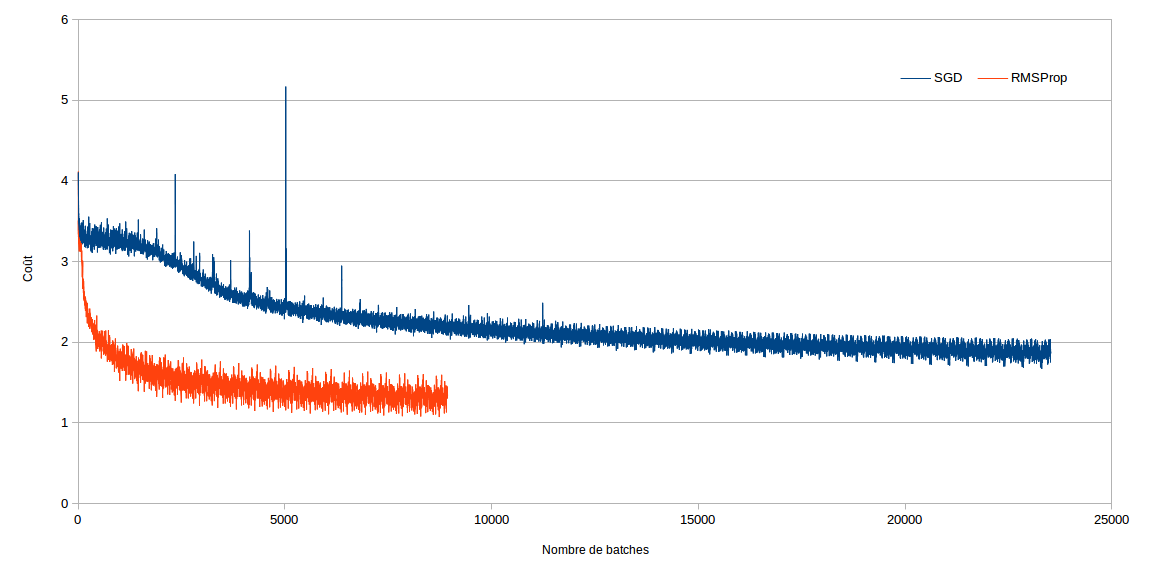
\includegraphics[scale=0.5]{images/chapter7/RMSProp_vs_SGD.png}
\caption{Courbe du coût lors de l'entrainement selon l'algorithme d'optimisation utilisé}
\label{RMSProp_vs_SGD}
\end{center}
\end{figure}
\medskip

Voici un exemple de texte généré:
\medbreak
Third Servan:\\
Of many bald with him fire, read now?\\

Second Murderer:\\
Out! where he wal’d apt thou, myself!\\
O brother’s maliss and trunks and Caubble subject.\\
Now i’ the fill in thy noble devart wagains to argon me
thy commanded?\\

LADY ANNE:\\
Sir, af you have fellow’s their eyes live?
\medbreak
Ces résultats, bien que durs à évaluer sont jugés satisfaisants étant donné leur ressemblance avec l'anglais shakespearien et leur structure de pièce de théâtre.
\\Il est intéressante de noter que certaines chaines de caractères comme les noms des personnages suivis de deux points et d'un retour à la ligne est copiée conformément exactement sur l'ensemble d'apprentissage, et dépend même de la pièce qui a été apprise en dernier.
\subsection{tests complémentaires sur la forget gate}
Le problème de la génération de texte a été l'occasion de questionner l'utilité de la forget gate. Cette partie de la cellule LSTM ne figurait que dans une partie des sources décrivant la composition de la cellule.
La question est de savoir si retirer cette porte diminue notablement l'efficacité du réseau, et ce même en ajoutant des neurones à la couche cachée pour garder un nombre de neurone constant par cellule.
\\ Le tracé de la courbe de coût lors de l'apprentissage (figure \ref{forget_gate} montre que la forget gate apporte effectivement un gain en performances.

\begin{figure}
\begin{center}
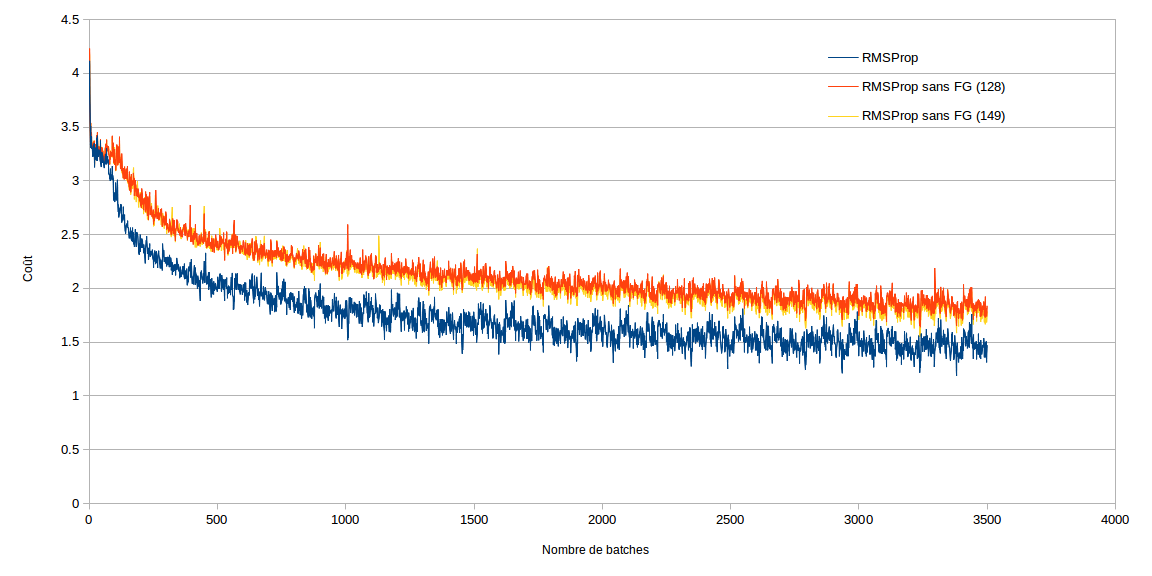
\includegraphics[scale=0.5]{images/chapter7/forget_gate.png}
\caption{Courbe du coût lors de l'entrainement avec avec ou sans forget gate}
\label{forget_gate}
\end{center}
\end{figure}


\section{Conclusion}
Une bonne utilisation des LSTM permet donc de générer un texte qu'on peut qualifier d'acceptable. Cependant mesurer la réussite de la génération est un problème à part entière qu'on ne traite pas ici, et les résultats sont donc difficilement quantifiables. De plus le texte produit semble en partie très proche du texte passé lors de la phase d'apprentissage.



\chapter{Algorithmes d'optimisation}
\section{Motivation}
Il existe une grande variété d'algorithmes permettant la minimisation de la fonction de coût autres que la descente de gradient présentée précédemment. Ce chapitre aura pour but de présenter les plus populaires d'entre eux et d'en donner les principales caractéristiques. Nous les comparerons ensuite pour retenir les solutions les plus efficaces.

Dans cette partie, la fonction de coût sera notée $J$ et les poids $W$.

\section{Descente de gradient et momentum}
\begin{equation}
W_{t+1} = W_t - \eta\frac{\partial J}{\partial W}
\end{equation} 

Les poids sont changés en fonction de la dérivée partielle de la fonction de coût par rapport à $W$. Comme vu précédemment, $\eta$ représente le learning rate. Si celui-ci est trop faible, la convergence sera lente, à l'inverse une valeur trop élevée entrainera la divergence des poids.

Cependant, le gradient de la fonction de coût change rapidement à chaque itération à cause de la diversité de chaque exemple d'apprentissage. On approchera alors le minimum par petits pas mais de façon désordonnée (en "zigzag"). En effet, si la direction moyenne obtenue sur plusieurs exemples d'apprentissage est la bonne ce n'est pas le cas si l'on ne prend en compte qu'un échantillon, celui-ci étant bruité. Cette approche consistant à calculer le gradient à chaque exemple est appelée \textit{descente de gradient stochastique}.

Pour pallier ce problème, deux solutions sont possibles. On peut moyenner le gradient sur des batches d'exemples de longueur fixée, au risque d'avoir de la redondance et de perdre en vitesse de calcul ou en espace mémoire. On parle alors de \textit{descente de gradient par batches}. La \textit{descente de gradient par mini-batches} consiste à prendre les avantages des deux méthodes, en trouvant un compromis sur la taille des batchs de sorte que le temps de calcul de chaque étape ne soit pas trop long mais que les pas soient suffisamment précis pour assurer une convergence efficace.

Il est également possible d'introduire un terme de momentum. Cette opération consiste à prendre en compte l'information des itérations précédentes pour savoir dans quelle direction il est préférable de progresser. En introduisant à cet effet un nouvel hyperparamètre $\mu$, on obtient alors les équations de mise à jour des poids ci-dessous.

\begin{equation}
\begin{aligned}
v_{t+1} = \mu v_t - \eta\frac{\partial J}{\partial W}\\
W_{t+1} = W_t + v_t
\end{aligned}
\end{equation} 

La trajectoire est alors plus lisse et la convergence plus efficace.

\section{Algorithmes à learning rate adaptatif}
\subsection{Adagrad}

L'objectif de cet algorithme est de ne plus avoir de learning rate constant mais d'adapter celui-ci en fonction de la valeur du gradient aux étapes précédentes. Cela se traduit dans l'équation de mise à jour des poids par une division par un terme $g_t$, somme des carrés des gradients des itérations précédentes.
On obtient finalement les équations suivantes :

\begin{equation}
\begin{aligned}
g_{t+1} = g_t + (\frac{\partial J}{\partial W})^2 \\
W_{t+1} = W_t - \dfrac{\eta\frac{\partial J}{\partial W}}{\sqrt{g_{t+1}} + \epsilon}
\end{aligned}
\end{equation} 

Le terme $\epsilon$ sert à initialiser l'algorithme et permet de s'assurer que le dénominateur ne sera jamais nul. On observe que si la norme du gradient est grande, le learning rate sera faible et vice versa. 
On n'a donc plus besoin de changer le learning rate manuellement, celui-ci est simplement fixé au départ puis adapté automatiquement. Cependant, comme le terme au dénominateur va augmenter au fur et à mesure, les termes $g_t$ étant tous positifs, le learning rate aura tendance à devenir de plus en plus faible jusqu'à devenir infinitésimal. Les algorithmes suivants permettront de résoudre ce problème.

\subsection{RMSProp}

La principale différence avec Adagrad est que le terme $g_t$ est calculé grâce à une moyenne mobile exponentielle : on utilise alors une pondération des termes qui décroît exponentiellement, ce qui donne plus d'importance aux valeurs récentes du gradient sans pour autant supprimer complètement les anciennes contributions. 

\begin{equation} 
\begin{aligned}
g_{t+1} = \gamma g_t + (1-\gamma)(\frac{\partial J}{\partial W})^2 \\
W_{t+1} = W_t - \dfrac{\eta\frac{\partial J}{\partial W}}{\sqrt{g_{t+1}} + \epsilon}
\end{aligned}
\end{equation} 

En raison du terme quadratique présent lors du calcul de $g_t$, ce dernier est appelé \textbf{moment d'ordre 2} de $\frac{\partial J}{\partial W}$. On trouve dans certaines implémentations l'ajout d'un moment d'ordre 1, qui se définit de façon très similaire par :
\begin{equation} 
m_{t+1} = \gamma m_t + (1-\gamma)(\frac{\partial J}{\partial W})
\end{equation} 

Il est même possible de rajouter un terme de momentum comme pour la descente du gradient stochastique, les équations de mise à jour finales sont alors :

\begin{equation} 
\begin{aligned}
v_{t+1} = \mu v_t - \dfrac{\eta \frac{\partial J}{\partial W}}{\sqrt{g_{t+1}-m^2_{t+1}+\epsilon}}\\
W_{t+1} = W_t + v_{t+1}
\end{aligned}
\end{equation} 

\subsection{Adadelta}

Cet algorithme utilise également une moyenne mobile exponentielle pour le calcul de $g_t$, moment d'ordre 2 du gradient. Cependant, au lieu d'utiliser un hyperparamètre $\eta$ fixe comme précédemment, il introduit à la place $x_t$, moment d'ordre 2 de $v_t$.

\begin{equation} 
\begin{aligned}
g_{t+1} = \gamma g_t + (1-\gamma) (\frac{\partial J}{\partial W})^2 \\
x_{t+1} = \gamma x_t + (1-\gamma)v^2_{t+1}
\end{aligned}
\end{equation}


Les équations finales sont alors, si l'on se limite aux moments d'ordre 2 et sans momentum :

\begin{equation}
\begin{aligned}
v_{t+1} = - \dfrac{\sqrt{x_t + \epsilon}\frac{\partial J}{\partial W}}{\sqrt{g_{t+1}+\epsilon}}\\
W_{t+1} = W_t + v_{t+1}
\end{aligned}
\end{equation}
 
\subsection{Adam}

Le dernier algorithme présenté consiste à reprendre les moments d'ordre 1 et 2 du gradient, $m_t$ et $g_t$, mais en les faisant cette fois-ci décroître dans le temps à l'aide de coefficients $\gamma_1$ et $\gamma_2$ $\in$ [0,1[

\begin{equation}
\begin{aligned}
\hat{m}_{t+1}=\dfrac{m_{t+1}}{1-\gamma^{t+1}_1}
\hat{g}_{t+1}=\dfrac{g_{t+1}}{1-\gamma^{t+1}_2}
\end{aligned}
\end{equation}

Cela aura donc pour effet de réduire la taille des pas à l'approche du minimum et donc d'assurer une bonne convergence grâce à une adaptation efficace du learning rate. On obtient finalement l'équation de mise à jour des poids suivante :

\begin{equation}
\begin{aligned}
W_{t+1}=W_t - \dfrac{\alpha\hat{m}_{t+1}}{\sqrt{\hat{g}_{t+1}}+\epsilon}
\end{aligned}
\end{equation}

\section{Comparaison des algorithmes}

Nous avons eu l'occasion d'implémenter ces différents algorithmes et de les appliquer aux problèmes précédents. S'il n'y a pas à l'heure actuelle de consensus sur le meilleur d'entre eux, certaines solutions se sont révélées être bien plus efficaces que d'autres dans notre cas.

\subsection{Application à l'apprentissage du XOR}

\begin{figure}[!h]
\begin{center}
	{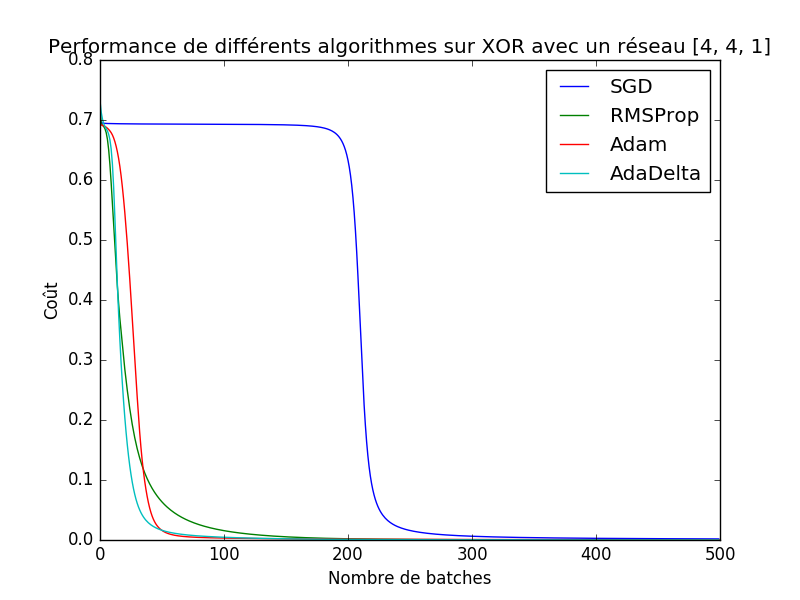
\includegraphics[scale=0.4]{images/chapter8/xor_comparison_algo.png}\label{Algorithmes}}
  \caption{Comparaison des fonctions de coût pour les différents algorithmes appliqués au XOR}
\end{center}
\end{figure}

On observe que les fonctions de coût pour les algorithmes à learning rate adaptatif ont des profils très similaires et ne présentent pas le pallier observé pour la descente de gradient stochastique. L'apprentissage est presque 4 fois plus rapide pour des temps de calcul du même ordre de grandeur, ce sont donc de meilleures implémentations en tout point pour ce type de problème.

\subsection{Application à l'apprentissage des oeuvres de Shakespeare}

\begin{figure}[!h]
\begin{center}
	{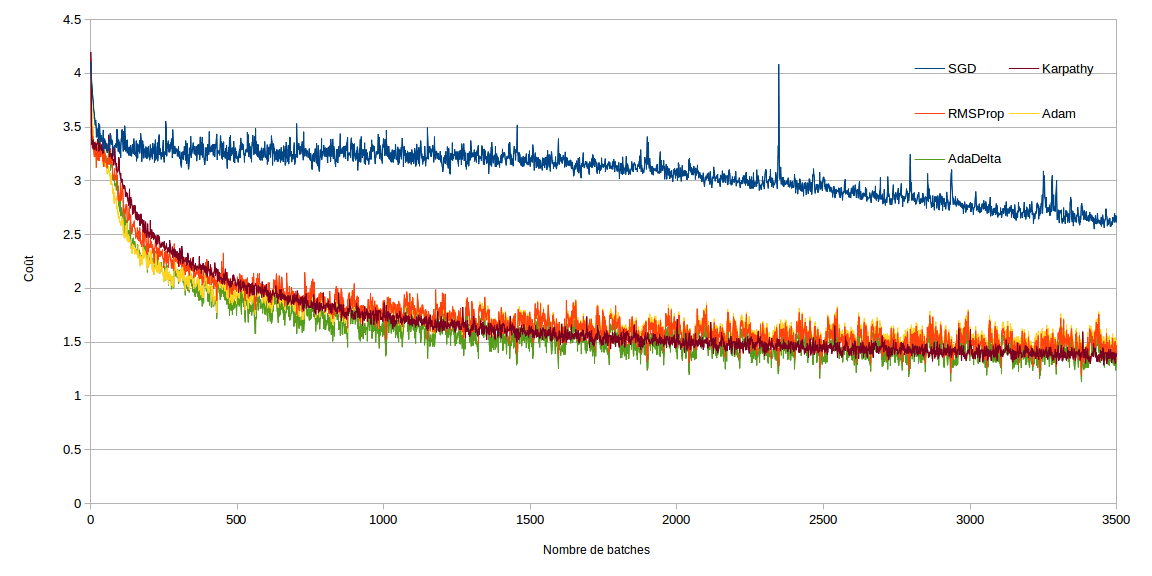
\includegraphics[scale=0.4]{images/chapter8/comparison.png}\label{Algorithmes}}
  \caption{Comparaison des fonctions de coût pour les différents algorithmes appliqués à Shakespeare aux côtés de l'implémentation d'Andrej Karpathy}
\end{center}
\end{figure}

La différence entre la descente de gradient stochastique et les autres algorithmes est encore plus flagrante dans ce cas : la convergence est bien plus rapide, nécessitant bien moins d'exemples d'apprentissage. Nous avons donc par la suite totalement délaissé la descente de gradient classique au profit de RMSProp ou Adam, beaucoup plus performants.

\section {Conclusion}
Si la descente du gradient stochastique est l'algorithme le plus répandu dans la littérature, il existe de nombreuses autres méthodes d'optimisation pour la minimisation de la fonction de coût. Nous avons présenté les plus populaires d'entre elles dans ce chapitre et avons réalisé qu'elles permettaient d'avoir de bien meilleures performances pour les applications que nous avons considérées. 

Il existe également une autre famille d'algorithmes du second ordre que nous n'avons pas eu le temps d'implémenter (méthode de Newton, BFGS, conjugate gradient...). Cependant, si nous avons trouvé des implémentations des algorithmes de ce chapitre dans des projets disponibles sur Internet, ce n'est pas le cas des méthodes du second ordre. Il est donc possible que ces dernières soient moins efficaces, que ce soit au niveau du temps de calcul ou de l'espace mémoire, bien que cela reste à vérifier.
\chapter{Application : génération de musique}

\section{Introduction}

La deuxième application des LSTM à laquelle nous nous sommes intéressés consistait en la génération de musique. Pour cela, nous avons envisagé quatre approches. La première n'est pas directement liée à la musique. En effet, on utilise alors le format abc qui représente un morceau de musique sous forme de texte. La génération se fait alors simplement en appliquant ce que l'on a fait avec Shakespeare. La deuxième méthode consiste à utiliser le format midi. Celui-ci permet de représenter simplement l'état des notes à chaque instant. La troisième méthode s'appuie sur l'utilisation de partitions qui permettent de retranscrire efficacement un morceau de musique. Dans ce cas-là, on génère directement une partition. Enfin, la dernière méthode consiste à exploiter un signal sonore. Cela permet d'utiliser tout type de son. \\
Quelle que soit la stratégie utilisée, il convient de trouver une base de données suffisamment fournie afin de pouvoir entraîner le réseau dessus. Il est assez difficile de trouver des fichiers abc sur différents styles de musique. En revanche, il existe plusieurs bases de données réunissant de nombreux fichiers midi. Enfin, l'utilisation de signaux permet de s'affranchir de ces problèmes puisqu'il est alors possible d'utiliser n'importe quel fichier sonore (wav, mp3, ...). Des convertisseurs existent afin de passer d'un format à l'autre, mais ceux-ci sont plus ou moins efficaces.

\section{Génération en abc}

\subsection{Présentation du format}

Le langage abc permet de représenter un morceau de musique en format ASCII. Il s'est rapidement développé grâce à sa facilité de représentation et de compatibilité entre les différents systèmes d'exploitation. De plus, ce langage ne nécessite pas l'utilisation d'un ordinateur pour être lu, contrairement au midi. Ainsi, les morceaux sont représentés de manière simple, efficace et compacte. \\
Un fichier abc est composé de deux parties : un entête et le corps de la musique.
L'entête permet de définir les caractéristiques globales du morceau :
\begin{itemize}
\item X : numéro du morceau dans le fichier
\item T : titre
\item M : valeur de la mesure
\item L : valeur de la note de référence
\item K : tonalité
\item P : ordre dans lequel les sections sont jouées
\end{itemize}
Le corps correspond à l'écriture du morceau. Les notes sont représentées dans le système anglo-saxon : a=la; b=si; c=do; d=ré; e=mi; f=fa; g=sol. Le choix des majuscules/minuscules et des symboles "," et "'" permettent de choisir les octaves utilisées. Les guillemets servent à écrire les accords. Les séparateurs sont utilisés pour les mesures et on peut spécifier les parties répétées. La figure \ref{fichier_abc_jig_exemple} est l'exemple d'une jig en format abc qui sera utilisée lors de l'apprentissage. 

\begin{figure}[!h]
\begin{verbatim}
X: 3
T:The American Dwarf
% Nottingham Music Database
S:FTB, via EF
M:6/8
K:D
P:A
A|"D" def fed|"G" BdB AFD| "D"DFA "G"B2 A|"Em" cee "A7" e2 A|
"D" def fed|"G" BdB "D"AFD|"D" DFA "G"B2 A|"A7" Add "D" d2:|
"B"e|"D"fga agf|"G" gab "A7"bag|"D"fga "D"agf|"Em" gfg "A7"e2 g|
"D"fga agf|"G"gab "A7"bag|"D" fga "A7"efg|"D" fdd d2 :|
\end{verbatim}
\caption{Exemple d'un fichier ABC}
\label{fichier_abc_jig_exemple}
\end{figure}

\subsection{Principe}
Étant donné que les morceaux de musique sont représentés sous forme de texte, on adopte un système d'apprentissage similaire à celui utilisé avec Shakespeare. \\
On utilise une cellule LSTM que l'on fait apprendre sur des séquences de longueur 50. Cela revient à déplier le réseau 50 fois à chaque apprentissage. Pour améliorer la rapidité et la convergence, on travaille avec des batchs de 50 séquences. L'algorithme d'optimisation choisi est RMSprop qui nous a donné les meilleurs résultats sur Shakespeare.

\subsection{Résultats}
Dans un premier temps, on réalise l'apprentissage sur un ensemble de 340 jigs trouvé sur une base de données de morceaux en abc. Le réseau arrive rapidement à apprendre la structure du format abc. De plus, les caractéristiques communes des jigs sont bien apprises; mélodie, accompagnement. La figure \ref{jig_generee_abc} est un exemple de jig générée avec notre réseau au format abc. Il existe des convertisseur abc/midi qui nous permettent de vérifier la cohérence du morceau généré. On voit ainsi que le réseau a très bien appris la structure des jigs, peut-être même trop bien, puisque certaines parties des morceaux générés sont quasiment identiques à des passages de la base de données d'apprentissage. Il arrive parfois que le texte généré présente quelques erreurs dans le format abc. Les convertisseurs sont en général capables de les corriger automatiquement voire d'ignorer les séquences absurdes.

\begin{figure}[!h]
\begin{verbatim}
X: 66
T:Pevim Dew's Music Datase
% Nottingham Music Database
S:Trae, arr Phil Rowe
M:6/8
K:G
D|"D"F2A fed|c2A "F"A2A|"G"g2a "F#m"a2a|"Am"a3 -F#7"B2c|
"C"c2c "G7"G2G|"C"EFG EFG|"D7"AGF c2d|"C7"e2c g2e|
"F"afA fed|"Dm" B2A c3| ^g=c "E7"Bcd|
"F"M3 c3|"D7"AFA dcA|"D"d2f a2f|"A7"agf abg|"D"baf d2d|"C"ede "G"dcB|
"D7"d2B c2A|"Gm"d2g "A7ec|edc BcA|"D""D"FAF "A"AFA|"D"FFD d2::
c|"Dm"d2e e3|"D7"dcB "F"dcf|
"G"f2d "A7"=g^c2|"D"d3 "A7"gef|
"A"f2e "A7"AFA|"D"def f2f|"D"a2d "A7"edc|"D"fdd cdd::
/2c/2|"D"a2f "G"d2f|"D"f2f "A7"gaf|"D"a2d "E7"cBA|A6|"D"Adc d2C|
[1"B7"BADFFAFA|"D"d, D "Cm"=c2c: [G"G2B-d2e|"F"a2e "C7/g""A7"^fe||
"D" "Dm"def "G/b"gge "D"f2B|"G"gfg gfg|edc AGG|"G"Bdg efd|"Am"eAA 
"D7"ABc|"G"B3 -B2B|Bdd G3:|
\end{verbatim}
\caption{Exemple d'une jig générée}
\label{jig_generee_abc}
\end{figure}

Cette méthode de génération est assez efficace et facile à mettre en oeuvre. Cependant, elle est assez limitée puisque l'on n'utilise qu'une représentation textuelle de la musique. Pour des morceaux plus complexes, comme Mozart, le réseaux a bien plus de mal à apprendre la structure de base du format. \\
On essaiera par la suite de proposer des méthodes d'apprentissage et de représentation des morceaux plus proches de la musique.

\section{Génération en midi}

\subsection{Présentation du format}

Le format midi utilise une représentation binaire. Un ensemble d'événements permet de décrire entièrement le morceau. On distingue les MetaMessages qui permettent de donner des informations d'ordre général sur la mélodie telles que le titre, la durée, le tempo, ... Il existe aussi les Messages qui décrivent la succession des événements tout au long du morceau, comme l'activation ou la désactivation de notes. Un morceau peut être décomposé en plusieurs tracks. Ceux-ci se partagent alors les différents voix : mélodie, accompagnement, ... 

On utilisera la bibliothèque $mido$ sous Python qui permet de représenter le format midi sous la forme d'une succession d'événements. Chaque message s'écrit alors de la manière suivante $événement\ paramètres\ time$. $time$ permet de définir après quel délai par rapport à l'événement précédent l'événement courant a lieu. Dans notre situation, on s'intéressera à l'exploitation des événements $note\_on\ note\ velocity\ time$ et $note\_off\ note\ velocity\ time$. Ceux-ci permettent d'activer ou de désactiver une note. On peut aussi préciser l'intensité de la note comprise entre 0 et 127. Dans notre cas, on considère que l'intensité vaut 0 lorsque l'on éteint la note. En réalité, elle permet de préciser de quelle manière on relâche la note (rapidement ou si on laisse un peu durer). Les notes sont elles aussi numéroter de 0 à 127. Le tableau \ref{tableau_notes} donne la correspondance entre les notes et leur numéro dans la représentation midi.

\begin{tiny}
\begin{center}
\begin{tabular}{|c|c|c|c|c|c|c|c|c|c|c|c|c|}
\hline
 & \multicolumn{12}{c|}{\textbf{Hauteurs}} \\
\hline
\textbf{Octave Number} & C & C\# & D & D\# & E & F & F\# & G & G\# & A & A\# & B  \\
\hline
0 & 0 & 1 & 2 & 3 & 4 & 5 & 6 & 7 & 8 & 9 & 10 & 11  \\
\hline
1 & 12 & 13 & 14 & 15 & 16 & 17 & 18 & 19 & 20 & 21 & 22 & 23  \\
\hline
2 & 24 & 25 & 26 & 27 & 28 & 29 & 30 & 31 & 32 & 33 & 34 & 35  \\
\hline
3 & 36 & 37 & 38 & 39 & 40 & 41 & 42 & 43 & 44 & 45 & 46 & 47  \\
\hline
4 & 48 & 49 & 50 & 51 & 52 & 53 & 54 & 55 & 56 & 57 & 58 & 59  \\
\hline
5 & 60 & 61 & 62 & 63 & 64 & 65 & 66 & 67 & 68 & 69 & 70 & 71  \\
\hline
6 & 72 & 73 & 74 & 75 & 76 & 77 & 78 & 79 & 80 & 81 & 82 & 83  \\
\hline
7 & 84 & 85 & 86 & 87 & 88 & 89 & 90 & 91 & 92 & 93 & 94 & 95  \\
\hline
8 & 96 & 97 & 98 & 99 & 100 & 101 & 102 & 103 & 104 & 105 & 106 & 107  \\
\hline
9 & 108 & 109 & 110 & 111 & 112 & 113 & 114 & 115 & 116 & 117 & 118 & 119  \\
\hline
10 & 120 & 121 & 122 & 123 & 124 & 125 & 126 & 127 &   &   &   & \\
\hline
\end{tabular}
\captionof{table}{Correspondance entre les notes et leur représentation en midi}
\label{tableau_notes}
\end{center}
\end{tiny}

\subsection{Principe}
Comme dit précédemment, on s'intéresse simplement à l'activation ou non de notes. Pour cela, nous allons représenter un morceau de musique par une matrice. Celle-ci possède 128 lignes (une pour chaque note) et à un nombre de colonnes dépendant de la longueur du morceau. En midi, un morceau est décomposé en ticks d'horloge. L'état du morceau variant peu entre deux ticks, il convient de le rééchantillonner afin d'avoir une matrice exploitable. Chaque instant sera ainsi décrit par une colonne de la matrice. En regardant chaque ligne, on pourra savoir si une note est éteinte (0) ou si elle est activé, on a alors directement accès à sa vélocité (entre 1 et 127). Dans notre représentation, nous décrirons tous les tracks dans une seule matrice.

Nous testerons notre implémentation sur les jigs déjà utilisées en abc après les avoir converties en midi (en utilisant abc2midi) ainsi que des morceaux de Mozart au piano. Les figures \ref{jig} et \ref{mozart} représentent les matrices d'une jig et d'un morceau de Mozart.

\begin{figure}[!h]
  \centering
  \subfloat[Jig]{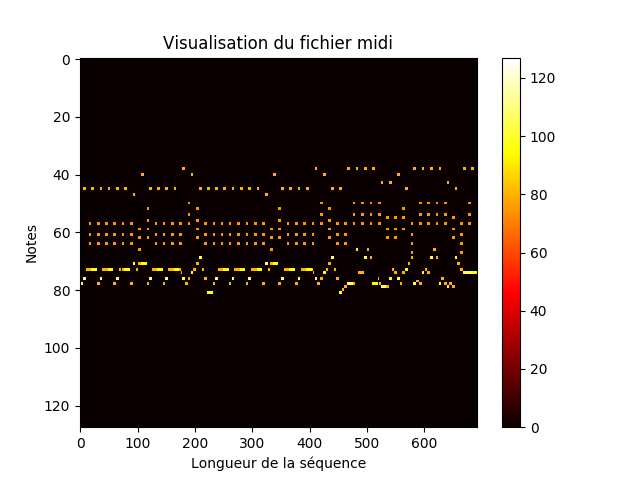
\includegraphics[width=0.5\textwidth]{images/chapter9/jig1.png}\label{jig}}
  \hfill
  \subfloat[Mozart]{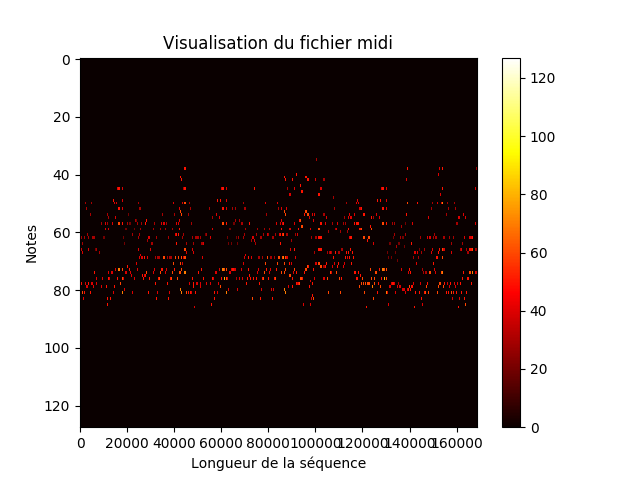
\includegraphics[width=0.5\textwidth]{images/chapter9/mozart.png}\label{mozart}}
  \caption{Visualisation de fichiers midi}
\end{figure}

Lors de l'apprentissage, on envoie en entrée du réseau une colonne de la matrice. Celui-ci doit alors prévoir la prochaine. Lors de la génération, on donne un vecteur ou une séquence de notes en entrée du réseau et on lui demande de générer un morceau de musique. On définit un seuil (à régler, souvent entre 10 et 20) qui permet de décider si une note est active ou non. Cela permet de jouer plusieurs notes en même temps ainsi que des accords. Après la génération d'un vecteur, on ne le remet pas directement en entrée. On sélectionne les notes actives grâce au seuil et on met les autres à 0. On obtient finalement un ensemble de vecteurs décrivant les états successifs du morceau généré. On les concatène pour en faire une matrice. Il ne reste plus qu'à faire la conversion de cette matrice en midi.


\subsection{Résultats}
On applique dans un premier temps l'apprentissage sur les jigs. On utilise deux cellules LSTM en série avec un état caché de 512. On met une couche de neurones pour adapter les données en sortie. Avec une activation linéaire on obtient ainsi des vecteurs de taille 128 en sortie où chaque élément représente l'intensité de la note correspondante. On lui donne en entrée des séquence de 10 vecteurs, cela signifie que l'on va déplier le réseau 10 fois à chaque fois. Un fait des batchs de 50 séquences. On utilise RMSprop comme algorithme d'optimisation avec un learning rate de 0.95. La figure \ref{midi_generated_jigs} permet de visualiser le fichier généré après le passage de 38 800 batchs lors de l'apprentissage.

\begin{figure}[!ht]
  \centering
  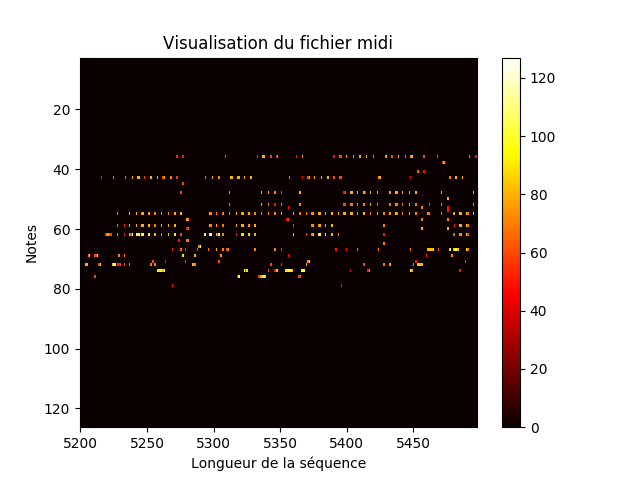
\includegraphics[width=0.5\textwidth]{images/chapter9/midi_generated_jigs_38800.png}
  \caption{Visualisation du fichier midi généré à partir des jigs après 38 800 batchs}
    \label{midi_generated_jigs}
\end{figure}
Le résultat obtenu possède bien le style des jigs avec un accompagnement répétitif à l'arrière. Cet accompagnement, souvent commun aux jigs, est très rapidement appris par le réseau. Certaines séquences mélodiques rappellent énormément certaines jigs de l'apprentissage.

\vspace{2cm}

L'apprentissage de Mozart se fait sur plusieurs symphonies pour piano trouvées dans une base de données de midi. On utilise une fois de plus 2 cellules LSTM en série avec un état caché de 512. Cette fois on fait l'apprentissage sur des séquences de longueur 120. Une longueur plus grande est importante car les morceaux de Mozart sont moins répétitifs que les jigs. Cela permet au réseau de remonter plus loin dans les vecteurs passés et donc d'apprendre la structure de séquences plus longues. On passe des batchs comportant 10 séquences. On utilise là aussi l'algorithme RMSprop avec un learning rate de 0.95. \\
La difficulté principale lors de l'apprentissage de Mozart est que la structure commune des morceaux est moins évidente que dans les jigs. De plus, il y a souvent des changements de rythmes/tempo dans les fichiers midi, ce qui est difficile à retranscrire dans la représentation matricielle avec l'implémentation actuelle. La figure \ref{midi_generated_mozart} représente le morceau généré après 79 500 passés.

\begin{figure}[!h]
  \centering
  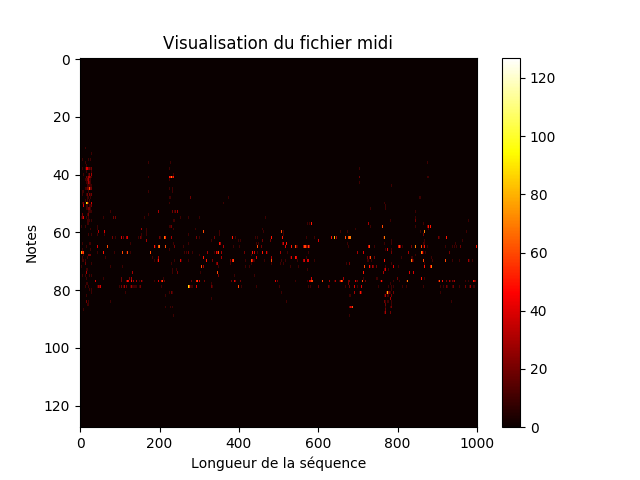
\includegraphics[width=0.5\textwidth]{images/chapter9/midi_generated_mozart_79500.png}
  \caption{Visualisation du fichier midi généré à partir des morceaux de Mozart après 79 500 batchs}
  \label{midi_generated_mozart}
\end{figure}

Il est nécessaire de passer un grand nombre de batchs avant d'avoir des résultats satisfaisants. Le morceau généré a une forme similaire aux morceaux du datasets. Néanmoins, l'écoute ne rend pas toujours aussi bien que les originaux. Un réseau plus complexe, un apprentissage plus long et une base de données plus importante pourraient permettre d'améliorer les résultats.


\section{Génération de partitions}

Dans cette partie, notre objectif est de générer des partitions de musique. Nous allons manipuler de la musique formellement. Les hauteurs des notes seront quantifiées, seules les hauteurs utilisées dans le solfège seront autorisées. De même pour les durées des notes, elles seront quantifiées.

Notre démarche a été de commencer simplement en générant seulement des notes pour un seul instrument puis de complexifier notre architecture afin de générer des notes pour plusieurs instruments.

L'ensemble de données utilisé pour l'apprentissage est principalement un ensemble de gigues. Cet ensemble a l'avantage d'être assez grand et les morceaux sont assez similaires entre eux ce qui facilite l'apprentissage du réseau. Quelques tentatives ont été effectuées sur d'autres ensembles de données mais leur petite taille ou manque de similarité n'a pas permis d'aboutir à des résultats concluants.

Dans toute cette partie, on utilise la bibliothèque \texttt{music21} qui permet de manipuler très aisément des partitions en Python. Elle permet entre autre de lire des fichiers dans les formats MIDI, ABC et MusicXML et fournit une représentation formelle des morceaux de musiques.

\subsection{Génération de notes}

La première étape dans la génération de partitions consiste à apprendre à un réseau à générer des suites de notes. Nous essaierons ensuite d'étendre l'architecture à plusieurs instruments.

\subsubsection{Architecture}

Nous modélisons une note comme une hauteur et une durée. On associe alors à une note un vecteur de $\mathbb{R}^{m+n}$ où :
\begin{itemize}
\item les $m$ premières dimensions servent à décrire la hauteur de la note ou un caractère spécial (silence, début d'un morceau, ...) ;
\item les $n$ suivantes la durée de la note.
\end{itemize}
Les deux parties sont \textit{one-hot-encoded} c'est-à-dire qu'elles contiennent un $1$ aux indices correspondants à la hauteur et à la durée de la note et des $0$ ailleurs.

Nous utilisons alors une architecture assez proche de celle présentée dans la partie \ref{chapter7}. Une représentation simplifiée est présente sur la figure \ref{note_rnn_simplified}.

\begin{figure}[h!]
\begin{center}
% Graphic for TeX using PGF
% Title: /home/pierre/Programming/pl-lstm/images/illustrations_cr/note_rnn_simplified.dia
% Creator: Dia v0.97.3
% CreationDate: Tue Jun 13 13:23:48 2017
% For: pierre
% \usepackage{tikz}
% The following commands are not supported in PSTricks at present
% We define them conditionally, so when they are implemented,
% this pgf file will use them.
\ifx\du\undefined
  \newlength{\du}
\fi
\setlength{\du}{15\unitlength}
\begin{tikzpicture}[scale=0.85]
\pgftransformxscale{1.000000}
\pgftransformyscale{-1.000000}
\definecolor{dialinecolor}{rgb}{0.000000, 0.000000, 0.000000}
\pgfsetstrokecolor{dialinecolor}
\definecolor{dialinecolor}{rgb}{1.000000, 1.000000, 1.000000}
\pgfsetfillcolor{dialinecolor}
\pgfsetlinewidth{0.100000\du}
\pgfsetdash{}{0pt}
\pgfsetdash{}{0pt}
\pgfsetroundjoin
{\pgfsetcornersarced{\pgfpoint{1.000000\du}{1.000000\du}}\definecolor{dialinecolor}{rgb}{0.882353, 0.968627, 0.815686}
\pgfsetfillcolor{dialinecolor}
\fill (10.000000\du,12.000000\du)--(10.000000\du,20.000000\du)--(24.000000\du,20.000000\du)--(24.000000\du,12.000000\du)--cycle;
}{\pgfsetcornersarced{\pgfpoint{1.000000\du}{1.000000\du}}\definecolor{dialinecolor}{rgb}{0.427451, 0.529412, 0.349020}
\pgfsetstrokecolor{dialinecolor}
\draw (10.000000\du,12.000000\du)--(10.000000\du,20.000000\du)--(24.000000\du,20.000000\du)--(24.000000\du,12.000000\du)--cycle;
}\pgfsetlinewidth{0.100000\du}
\pgfsetdash{}{0pt}
\pgfsetdash{}{0pt}
\pgfsetbuttcap
{
\definecolor{dialinecolor}{rgb}{0.000000, 0.000000, 0.000000}
\pgfsetfillcolor{dialinecolor}
% was here!!!
\pgfsetarrowsend{latex}
\definecolor{dialinecolor}{rgb}{0.000000, 0.000000, 0.000000}
\pgfsetstrokecolor{dialinecolor}
\draw (21.000000\du,12.000000\du)--(21.000000\du,10.000000\du);
}
\pgfsetlinewidth{0.100000\du}
\pgfsetdash{}{0pt}
\pgfsetdash{}{0pt}
\pgfsetbuttcap
{
\definecolor{dialinecolor}{rgb}{0.000000, 0.000000, 0.000000}
\pgfsetfillcolor{dialinecolor}
% was here!!!
\pgfsetarrowsend{latex}
\definecolor{dialinecolor}{rgb}{0.000000, 0.000000, 0.000000}
\pgfsetstrokecolor{dialinecolor}
\draw (24.000000\du,16.000000\du)--(28.000000\du,16.000000\du);
}
% setfont left to latex
\definecolor{dialinecolor}{rgb}{0.000000, 0.000000, 0.000000}
\pgfsetstrokecolor{dialinecolor}
\node at (8.000000\du,15.293750\du){$H(t-1)$};
\pgfsetlinewidth{0.100000\du}
\pgfsetdash{}{0pt}
\pgfsetdash{}{0pt}
\pgfsetbuttcap
{
\definecolor{dialinecolor}{rgb}{0.000000, 0.000000, 0.000000}
\pgfsetfillcolor{dialinecolor}
% was here!!!
\pgfsetarrowsend{latex}
\definecolor{dialinecolor}{rgb}{0.000000, 0.000000, 0.000000}
\pgfsetstrokecolor{dialinecolor}
\draw (12.000000\du,22.000000\du)--(12.000000\du,20.000000\du);
}
% setfont left to latex
\definecolor{dialinecolor}{rgb}{0.000000, 0.000000, 0.000000}
\pgfsetstrokecolor{dialinecolor}
\node at (26.000000\du,15.293750\du){$H(t)$};
% setfont left to latex
\definecolor{dialinecolor}{rgb}{0.000000, 0.000000, 0.000000}
\pgfsetstrokecolor{dialinecolor}
\node at (14.000000\du,21.293750\du){$X(t)$};
% setfont left to latex
\definecolor{dialinecolor}{rgb}{0.000000, 0.000000, 0.000000}
\pgfsetstrokecolor{dialinecolor}
\node at (17.000000\du,16.391250\du){LSTMs};
\pgfsetlinewidth{0.100000\du}
\pgfsetdash{}{0pt}
\pgfsetdash{}{0pt}
\pgfsetbuttcap
{
\definecolor{dialinecolor}{rgb}{0.000000, 0.000000, 0.000000}
\pgfsetfillcolor{dialinecolor}
% was here!!!
\pgfsetarrowsend{latex}
\definecolor{dialinecolor}{rgb}{0.000000, 0.000000, 0.000000}
\pgfsetstrokecolor{dialinecolor}
\draw (6.000000\du,16.000000\du)--(10.000000\du,16.000000\du);
}
% setfont left to latex
\definecolor{dialinecolor}{rgb}{0.000000, 0.000000, 0.000000}
\pgfsetstrokecolor{dialinecolor}
\node at (23.000000\du,11.293750\du){$Y(t)$};
\pgfsetlinewidth{0.100000\du}
\pgfsetdash{}{0pt}
\pgfsetdash{}{0pt}
\pgfsetmiterjoin
\definecolor{dialinecolor}{rgb}{0.960784, 0.933333, 0.611765}
\pgfsetfillcolor{dialinecolor}
\fill (7.500000\du,22.000000\du)--(7.500000\du,24.000000\du)--(12.500000\du,24.000000\du)--(12.500000\du,22.000000\du)--cycle;
\definecolor{dialinecolor}{rgb}{0.000000, 0.000000, 0.000000}
\pgfsetstrokecolor{dialinecolor}
\draw (7.500000\du,22.000000\du)--(7.500000\du,24.000000\du)--(12.500000\du,24.000000\du)--(12.500000\du,22.000000\du)--cycle;
\pgfsetlinewidth{0.100000\du}
\pgfsetdash{}{0pt}
\pgfsetdash{}{0pt}
\pgfsetmiterjoin
\definecolor{dialinecolor}{rgb}{0.960784, 0.933333, 0.611765}
\pgfsetfillcolor{dialinecolor}
\fill (12.500000\du,22.000000\du)--(12.500000\du,24.000000\du)--(16.500000\du,24.000000\du)--(16.500000\du,22.000000\du)--cycle;
\definecolor{dialinecolor}{rgb}{0.000000, 0.000000, 0.000000}
\pgfsetstrokecolor{dialinecolor}
\draw (12.500000\du,22.000000\du)--(12.500000\du,24.000000\du)--(16.500000\du,24.000000\du)--(16.500000\du,22.000000\du)--cycle;
% setfont left to latex
\definecolor{dialinecolor}{rgb}{0.000000, 0.000000, 0.000000}
\pgfsetstrokecolor{dialinecolor}
\node at (10.000000\du,23.222500\du){Hauteur(t)};
% setfont left to latex
\definecolor{dialinecolor}{rgb}{0.000000, 0.000000, 0.000000}
\pgfsetstrokecolor{dialinecolor}
\node at (14.500000\du,23.222500\du){Durée(t)};
\pgfsetlinewidth{0.100000\du}
\pgfsetdash{}{0pt}
\pgfsetdash{}{0pt}
\pgfsetmiterjoin
\definecolor{dialinecolor}{rgb}{0.960784, 0.933333, 0.611765}
\pgfsetfillcolor{dialinecolor}
\fill (16.500000\du,8.000000\du)--(16.500000\du,10.000000\du)--(21.500000\du,10.000000\du)--(21.500000\du,8.000000\du)--cycle;
\definecolor{dialinecolor}{rgb}{0.000000, 0.000000, 0.000000}
\pgfsetstrokecolor{dialinecolor}
\draw (16.500000\du,8.000000\du)--(16.500000\du,10.000000\du)--(21.500000\du,10.000000\du)--(21.500000\du,8.000000\du)--cycle;
\pgfsetlinewidth{0.100000\du}
\pgfsetdash{}{0pt}
\pgfsetdash{}{0pt}
\pgfsetmiterjoin
\definecolor{dialinecolor}{rgb}{0.960784, 0.933333, 0.611765}
\pgfsetfillcolor{dialinecolor}
\fill (21.500000\du,8.000000\du)--(21.500000\du,10.000000\du)--(25.500000\du,10.000000\du)--(25.500000\du,8.000000\du)--cycle;
\definecolor{dialinecolor}{rgb}{0.000000, 0.000000, 0.000000}
\pgfsetstrokecolor{dialinecolor}
\draw (21.500000\du,8.000000\du)--(21.500000\du,10.000000\du)--(25.500000\du,10.000000\du)--(25.500000\du,8.000000\du)--cycle;
% setfont left to latex
\definecolor{dialinecolor}{rgb}{0.000000, 0.000000, 0.000000}
\pgfsetstrokecolor{dialinecolor}
\node at (19.000000\du,9.222500\du){Hauteur(t+1)};
% setfont left to latex
\definecolor{dialinecolor}{rgb}{0.000000, 0.000000, 0.000000}
\pgfsetstrokecolor{dialinecolor}
\node at (23.500000\du,9.222500\du){Durée(t+1)};
\end{tikzpicture}

\caption{Architecture du réseau utilisé pour la génération de notes.}
\label{note_rnn_simplified}
\end{center}
\end{figure}

Il existe cependant une différence car il est nécessaire de générer une hauteur et une durée et non plus seulement un caractère comme dans la partie \ref{chapter7}. Afin de réaliser cela, on utilise deux fois la fonction $softmax$ en sortie. Une fois sur les $m$ premières coordonnées et une autre fois sur les $n$ dernières coordonnées. Il faut alors changer la fonction de coût de manière correspondante : on utilise la fonction de coût $softmaxCE$ indépendamment pour les deux parties du vecteur de sortie. On retrouvera un schéma détaillé de cette architecture sur la figure \ref{note_rnn}. Cette modélisation permet d'apprendre deux distribution de probabilités : une pour la hauteur et une pour la durée. Il faut noter que ces distributions de probabilités sont dépendantes car générées à partir de la sortie de la cellule LSTM.

\begin{figure}[h!]
\begin{center}
% Graphic for TeX using PGF
% Title: /home/pierre/Programming/pl-lstm/images/illustrations_cr/note_rnn.dia
% Creator: Dia v0.97.3
% CreationDate: Tue Jun 13 13:19:05 2017
% For: pierre
% \usepackage{tikz}
% The following commands are not supported in PSTricks at present
% We define them conditionally, so when they are implemented,
% this pgf file will use them.
\ifx\du\undefined
  \newlength{\du}
\fi
\setlength{\du}{15\unitlength}
\begin{tikzpicture}[scale=0.8]
\pgftransformxscale{1.000000}
\pgftransformyscale{-1.000000}
\definecolor{dialinecolor}{rgb}{0.000000, 0.000000, 0.000000}
\pgfsetstrokecolor{dialinecolor}
\definecolor{dialinecolor}{rgb}{1.000000, 1.000000, 1.000000}
\pgfsetfillcolor{dialinecolor}
\pgfsetlinewidth{0.100000\du}
\pgfsetdash{}{0pt}
\pgfsetdash{}{0pt}
\pgfsetroundjoin
{\pgfsetcornersarced{\pgfpoint{1.000000\du}{1.000000\du}}\definecolor{dialinecolor}{rgb}{0.882353, 0.968627, 0.815686}
\pgfsetfillcolor{dialinecolor}
\fill (10.000000\du,12.000000\du)--(10.000000\du,20.000000\du)--(24.000000\du,20.000000\du)--(24.000000\du,12.000000\du)--cycle;
}{\pgfsetcornersarced{\pgfpoint{1.000000\du}{1.000000\du}}\definecolor{dialinecolor}{rgb}{0.427451, 0.529412, 0.349020}
\pgfsetstrokecolor{dialinecolor}
\draw (10.000000\du,12.000000\du)--(10.000000\du,20.000000\du)--(24.000000\du,20.000000\du)--(24.000000\du,12.000000\du)--cycle;
}\pgfsetlinewidth{0.100000\du}
\pgfsetdash{}{0pt}
\pgfsetdash{}{0pt}
\pgfsetbuttcap
{
\definecolor{dialinecolor}{rgb}{0.000000, 0.000000, 0.000000}
\pgfsetfillcolor{dialinecolor}
% was here!!!
\definecolor{dialinecolor}{rgb}{0.000000, 0.000000, 0.000000}
\pgfsetstrokecolor{dialinecolor}
\draw (6.000000\du,14.000000\du)--(10.000000\du,14.000000\du);
}
\pgfsetlinewidth{0.100000\du}
\pgfsetdash{}{0pt}
\pgfsetdash{}{0pt}
\pgfsetbuttcap
{
\definecolor{dialinecolor}{rgb}{0.000000, 0.000000, 0.000000}
\pgfsetfillcolor{dialinecolor}
% was here!!!
\pgfsetarrowsend{latex}
\definecolor{dialinecolor}{rgb}{0.000000, 0.000000, 0.000000}
\pgfsetstrokecolor{dialinecolor}
\draw (24.000000\du,14.000000\du)--(28.000000\du,14.000000\du);
}
\pgfsetlinewidth{0.100000\du}
\pgfsetdash{}{0pt}
\pgfsetdash{}{0pt}
\pgfsetbuttcap
{
\definecolor{dialinecolor}{rgb}{0.000000, 0.000000, 0.000000}
\pgfsetfillcolor{dialinecolor}
% was here!!!
\definecolor{dialinecolor}{rgb}{0.000000, 0.000000, 0.000000}
\pgfsetstrokecolor{dialinecolor}
\draw (21.000000\du,12.000000\du)--(21.000000\du,11.000000\du);
}
\pgfsetlinewidth{0.100000\du}
\pgfsetdash{}{0pt}
\pgfsetdash{}{0pt}
\pgfsetbuttcap
{
\definecolor{dialinecolor}{rgb}{0.000000, 0.000000, 0.000000}
\pgfsetfillcolor{dialinecolor}
% was here!!!
\pgfsetarrowsend{latex}
\definecolor{dialinecolor}{rgb}{0.000000, 0.000000, 0.000000}
\pgfsetstrokecolor{dialinecolor}
\draw (24.000000\du,19.000000\du)--(28.000000\du,19.000000\du);
}
% setfont left to latex
\definecolor{dialinecolor}{rgb}{0.000000, 0.000000, 0.000000}
\pgfsetstrokecolor{dialinecolor}
\node at (8.000000\du,13.391250\du){$S(t-1)$};
% setfont left to latex
\definecolor{dialinecolor}{rgb}{0.000000, 0.000000, 0.000000}
\pgfsetstrokecolor{dialinecolor}
\node at (26.000000\du,13.391250\du){$S(t)$};
% setfont left to latex
\definecolor{dialinecolor}{rgb}{0.000000, 0.000000, 0.000000}
\pgfsetstrokecolor{dialinecolor}
\node at (8.000000\du,18.391250\du){$H(t-1)$};
\pgfsetlinewidth{0.100000\du}
\pgfsetdash{}{0pt}
\pgfsetdash{}{0pt}
\pgfsetbuttcap
{
\definecolor{dialinecolor}{rgb}{0.000000, 0.000000, 0.000000}
\pgfsetfillcolor{dialinecolor}
% was here!!!
\definecolor{dialinecolor}{rgb}{0.000000, 0.000000, 0.000000}
\pgfsetstrokecolor{dialinecolor}
\draw (12.000000\du,23.000000\du)--(12.000000\du,20.000000\du);
}
% setfont left to latex
\definecolor{dialinecolor}{rgb}{0.000000, 0.000000, 0.000000}
\pgfsetstrokecolor{dialinecolor}
\node at (26.000000\du,18.391250\du){$H(t)$};
% setfont left to latex
\definecolor{dialinecolor}{rgb}{0.000000, 0.000000, 0.000000}
\pgfsetstrokecolor{dialinecolor}
\node at (14.000000\du,22.391250\du){$X(t)$};
% setfont left to latex
\definecolor{dialinecolor}{rgb}{0.000000, 0.000000, 0.000000}
\pgfsetstrokecolor{dialinecolor}
\node at (17.000000\du,16.391250\du){LSTMs};
\pgfsetlinewidth{0.100000\du}
\pgfsetdash{}{0pt}
\pgfsetdash{}{0pt}
\pgfsetmiterjoin
\pgfsetbuttcap
{
\definecolor{dialinecolor}{rgb}{0.000000, 0.000000, 0.000000}
\pgfsetfillcolor{dialinecolor}
% was here!!!
\pgfsetarrowsend{latex}
\definecolor{dialinecolor}{rgb}{0.000000, 0.000000, 0.000000}
\pgfsetstrokecolor{dialinecolor}
\pgfpathmoveto{\pgfpoint{21.000000\du}{11.000000\du}}
\pgfpathcurveto{\pgfpoint{21.000000\du}{9.000000\du}}{\pgfpoint{24.000000\du}{9.000000\du}}{\pgfpoint{24.000000\du}{7.000000\du}}
\pgfusepath{stroke}
}
\pgfsetlinewidth{0.100000\du}
\pgfsetdash{}{0pt}
\pgfsetdash{}{0pt}
\pgfsetmiterjoin
\pgfsetbuttcap
{
\definecolor{dialinecolor}{rgb}{0.000000, 0.000000, 0.000000}
\pgfsetfillcolor{dialinecolor}
% was here!!!
\pgfsetarrowsend{latex}
\definecolor{dialinecolor}{rgb}{0.000000, 0.000000, 0.000000}
\pgfsetstrokecolor{dialinecolor}
\pgfpathmoveto{\pgfpoint{21.000000\du}{11.000000\du}}
\pgfpathcurveto{\pgfpoint{21.000000\du}{9.000000\du}}{\pgfpoint{18.000000\du}{9.000000\du}}{\pgfpoint{18.000000\du}{7.000000\du}}
\pgfusepath{stroke}
}
\pgfsetlinewidth{0.100000\du}
\pgfsetdash{}{0pt}
\pgfsetdash{}{0pt}
\pgfsetbuttcap
{
\definecolor{dialinecolor}{rgb}{0.000000, 0.000000, 0.000000}
\pgfsetfillcolor{dialinecolor}
% was here!!!
\definecolor{dialinecolor}{rgb}{0.000000, 0.000000, 0.000000}
\pgfsetstrokecolor{dialinecolor}
\draw (6.000000\du,19.000000\du)--(10.000000\du,19.000000\du);
}
% setfont left to latex
\definecolor{dialinecolor}{rgb}{0.000000, 0.000000, 0.000000}
\pgfsetstrokecolor{dialinecolor}
\node at (23.000000\du,11.391250\du){$H(t)$};
\pgfsetlinewidth{0.100000\du}
\pgfsetdash{}{0pt}
\pgfsetdash{}{0pt}
\pgfsetmiterjoin
\definecolor{dialinecolor}{rgb}{0.960784, 0.933333, 0.611765}
\pgfsetfillcolor{dialinecolor}
\fill (16.000000\du,5.000000\du)--(16.000000\du,7.000000\du)--(20.000000\du,7.000000\du)--(20.000000\du,5.000000\du)--cycle;
\definecolor{dialinecolor}{rgb}{0.000000, 0.000000, 0.000000}
\pgfsetstrokecolor{dialinecolor}
\draw (16.000000\du,5.000000\du)--(16.000000\du,7.000000\du)--(20.000000\du,7.000000\du)--(20.000000\du,5.000000\du)--cycle;
% setfont left to latex
\definecolor{dialinecolor}{rgb}{0.000000, 0.000000, 0.000000}
\pgfsetstrokecolor{dialinecolor}
\node at (18.000000\du,6.293750\du){Softmax};
\pgfsetlinewidth{0.100000\du}
\pgfsetdash{}{0pt}
\pgfsetdash{}{0pt}
\pgfsetmiterjoin
\definecolor{dialinecolor}{rgb}{0.960784, 0.933333, 0.611765}
\pgfsetfillcolor{dialinecolor}
\fill (22.000000\du,5.000000\du)--(22.000000\du,7.000000\du)--(26.000000\du,7.000000\du)--(26.000000\du,5.000000\du)--cycle;
\definecolor{dialinecolor}{rgb}{0.000000, 0.000000, 0.000000}
\pgfsetstrokecolor{dialinecolor}
\draw (22.000000\du,5.000000\du)--(22.000000\du,7.000000\du)--(26.000000\du,7.000000\du)--(26.000000\du,5.000000\du)--cycle;
% setfont left to latex
\definecolor{dialinecolor}{rgb}{0.000000, 0.000000, 0.000000}
\pgfsetstrokecolor{dialinecolor}
\node at (24.000000\du,6.293750\du){Softmax};
\pgfsetlinewidth{0.100000\du}
\pgfsetdash{}{0pt}
\pgfsetdash{}{0pt}
\pgfsetmiterjoin
\pgfsetbuttcap
{
\definecolor{dialinecolor}{rgb}{0.000000, 0.000000, 0.000000}
\pgfsetfillcolor{dialinecolor}
% was here!!!
\definecolor{dialinecolor}{rgb}{0.000000, 0.000000, 0.000000}
\pgfsetstrokecolor{dialinecolor}
\pgfpathmoveto{\pgfpoint{24.000000\du}{5.000000\du}}
\pgfpathcurveto{\pgfpoint{24.000000\du}{3.000000\du}}{\pgfpoint{21.000000\du}{3.000000\du}}{\pgfpoint{21.000000\du}{1.000000\du}}
\pgfusepath{stroke}
}
\pgfsetlinewidth{0.100000\du}
\pgfsetdash{}{0pt}
\pgfsetdash{}{0pt}
\pgfsetmiterjoin
\pgfsetbuttcap
{
\definecolor{dialinecolor}{rgb}{0.000000, 0.000000, 0.000000}
\pgfsetfillcolor{dialinecolor}
% was here!!!
\definecolor{dialinecolor}{rgb}{0.000000, 0.000000, 0.000000}
\pgfsetstrokecolor{dialinecolor}
\pgfpathmoveto{\pgfpoint{21.000000\du}{1.000000\du}}
\pgfpathcurveto{\pgfpoint{21.000000\du}{3.000000\du}}{\pgfpoint{18.000000\du}{3.000000\du}}{\pgfpoint{18.000000\du}{5.000000\du}}
\pgfusepath{stroke}
}
\pgfsetlinewidth{0.100000\du}
\pgfsetdash{}{0pt}
\pgfsetdash{}{0pt}
\pgfsetbuttcap
{
\definecolor{dialinecolor}{rgb}{0.000000, 0.000000, 0.000000}
\pgfsetfillcolor{dialinecolor}
% was here!!!
\pgfsetarrowsend{latex}
\definecolor{dialinecolor}{rgb}{0.000000, 0.000000, 0.000000}
\pgfsetstrokecolor{dialinecolor}
\draw (21.000000\du,1.000000\du)--(21.000000\du,-8.000000\du);
}
\pgfsetlinewidth{0.100000\du}
\pgfsetdash{}{0pt}
\pgfsetdash{}{0pt}
\pgfsetmiterjoin
\pgfsetbuttcap
{
\definecolor{dialinecolor}{rgb}{0.000000, 0.000000, 0.000000}
\pgfsetfillcolor{dialinecolor}
% was here!!!
\pgfsetarrowsend{latex}
\definecolor{dialinecolor}{rgb}{0.000000, 0.000000, 0.000000}
\pgfsetstrokecolor{dialinecolor}
\pgfpathmoveto{\pgfpoint{18.000000\du}{5.000000\du}}
\pgfpathcurveto{\pgfpoint{18.000000\du}{3.000000\du}}{\pgfpoint{9.302992\du}{4.514959\du}}{\pgfpoint{8.802992\du}{2.014959\du}}
\pgfusepath{stroke}
}
\definecolor{dialinecolor}{rgb}{0.976471, 0.819608, 0.819608}
\pgfsetfillcolor{dialinecolor}
\pgfpathellipse{\pgfpoint{8.500000\du}{0.500000\du}}{\pgfpoint{1.500000\du}{0\du}}{\pgfpoint{0\du}{1.500000\du}}
\pgfusepath{fill}
\pgfsetlinewidth{0.100000\du}
\pgfsetdash{}{0pt}
\pgfsetdash{}{0pt}
\definecolor{dialinecolor}{rgb}{0.000000, 0.000000, 0.000000}
\pgfsetstrokecolor{dialinecolor}
\pgfpathellipse{\pgfpoint{8.500000\du}{0.500000\du}}{\pgfpoint{1.500000\du}{0\du}}{\pgfpoint{0\du}{1.500000\du}}
\pgfusepath{stroke}
\pgfsetlinewidth{0.100000\du}
\pgfsetdash{}{0pt}
\pgfsetdash{}{0pt}
\pgfsetmiterjoin
\pgfsetbuttcap
{
\definecolor{dialinecolor}{rgb}{0.000000, 0.000000, 0.000000}
\pgfsetfillcolor{dialinecolor}
% was here!!!
\pgfsetarrowsend{latex}
\definecolor{dialinecolor}{rgb}{0.000000, 0.000000, 0.000000}
\pgfsetstrokecolor{dialinecolor}
\pgfpathmoveto{\pgfpoint{24.000000\du}{5.000000\du}}
\pgfpathcurveto{\pgfpoint{24.000000\du}{3.000000\du}}{\pgfpoint{14.303018\du}{4.515090\du}}{\pgfpoint{13.803018\du}{2.015090\du}}
\pgfusepath{stroke}
}
\definecolor{dialinecolor}{rgb}{0.976471, 0.819608, 0.819608}
\pgfsetfillcolor{dialinecolor}
\pgfpathellipse{\pgfpoint{13.500000\du}{0.500000\du}}{\pgfpoint{1.500000\du}{0\du}}{\pgfpoint{0\du}{1.500000\du}}
\pgfusepath{fill}
\pgfsetlinewidth{0.100000\du}
\pgfsetdash{}{0pt}
\pgfsetdash{}{0pt}
\definecolor{dialinecolor}{rgb}{0.000000, 0.000000, 0.000000}
\pgfsetstrokecolor{dialinecolor}
\pgfpathellipse{\pgfpoint{13.500000\du}{0.500000\du}}{\pgfpoint{1.500000\du}{0\du}}{\pgfpoint{0\du}{1.500000\du}}
\pgfusepath{stroke}
% setfont left to latex
\definecolor{dialinecolor}{rgb}{0.000000, 0.000000, 0.000000}
\pgfsetstrokecolor{dialinecolor}
\node at (8.500000\du,0.793750\du){SCE};
% setfont left to latex
\definecolor{dialinecolor}{rgb}{0.000000, 0.000000, 0.000000}
\pgfsetstrokecolor{dialinecolor}
\node at (13.500000\du,0.793750\du){SCE};
\definecolor{dialinecolor}{rgb}{0.976471, 0.819608, 0.819608}
\pgfsetfillcolor{dialinecolor}
\pgfpathellipse{\pgfpoint{11.000000\du}{-5.000000\du}}{\pgfpoint{1.500000\du}{0\du}}{\pgfpoint{0\du}{1.500000\du}}
\pgfusepath{fill}
\pgfsetlinewidth{0.100000\du}
\pgfsetdash{}{0pt}
\pgfsetdash{}{0pt}
\definecolor{dialinecolor}{rgb}{0.000000, 0.000000, 0.000000}
\pgfsetstrokecolor{dialinecolor}
\pgfpathellipse{\pgfpoint{11.000000\du}{-5.000000\du}}{\pgfpoint{1.500000\du}{0\du}}{\pgfpoint{0\du}{1.500000\du}}
\pgfusepath{stroke}
% setfont left to latex
\definecolor{dialinecolor}{rgb}{0.000000, 0.000000, 0.000000}
\pgfsetstrokecolor{dialinecolor}
\node at (11.000000\du,-4.706250\du){$+$};
\pgfsetlinewidth{0.100000\du}
\pgfsetdash{}{0pt}
\pgfsetdash{}{0pt}
\pgfsetmiterjoin
\pgfsetbuttcap
{
\definecolor{dialinecolor}{rgb}{0.000000, 0.000000, 0.000000}
\pgfsetfillcolor{dialinecolor}
% was here!!!
\pgfsetarrowsend{latex}
\definecolor{dialinecolor}{rgb}{0.000000, 0.000000, 0.000000}
\pgfsetstrokecolor{dialinecolor}
\pgfpathmoveto{\pgfpoint{8.989985\du}{-0.969954\du}}
\pgfpathcurveto{\pgfpoint{9.489985\du}{-2.469954\du}}{\pgfpoint{9.307057\du}{-1.614114\du}}{\pgfpoint{10.307057\du}{-3.614114\du}}
\pgfusepath{stroke}
}
\pgfsetlinewidth{0.100000\du}
\pgfsetdash{}{0pt}
\pgfsetdash{}{0pt}
\pgfsetmiterjoin
\pgfsetbuttcap
{
\definecolor{dialinecolor}{rgb}{0.000000, 0.000000, 0.000000}
\pgfsetfillcolor{dialinecolor}
% was here!!!
\pgfsetarrowsend{latex}
\definecolor{dialinecolor}{rgb}{0.000000, 0.000000, 0.000000}
\pgfsetstrokecolor{dialinecolor}
\pgfpathmoveto{\pgfpoint{13.010015\du}{-0.969954\du}}
\pgfpathcurveto{\pgfpoint{12.510015\du}{-2.469954\du}}{\pgfpoint{12.692943\du}{-1.614114\du}}{\pgfpoint{11.692943\du}{-3.614114\du}}
\pgfusepath{stroke}
}
\pgfsetlinewidth{0.100000\du}
\pgfsetdash{}{0pt}
\pgfsetdash{}{0pt}
\pgfsetmiterjoin
\pgfsetbuttcap
{
\definecolor{dialinecolor}{rgb}{0.000000, 0.000000, 0.000000}
\pgfsetfillcolor{dialinecolor}
% was here!!!
\pgfsetarrowsend{latex}
\definecolor{dialinecolor}{rgb}{0.000000, 0.000000, 0.000000}
\pgfsetstrokecolor{dialinecolor}
\pgfpathmoveto{\pgfpoint{6.000000\du}{4.000000\du}}
\pgfpathcurveto{\pgfpoint{8.490000\du}{4.000000\du}}{\pgfpoint{8.000000\du}{4.000000\du}}{\pgfpoint{8.500000\du}{2.000000\du}}
\pgfusepath{stroke}
}
\pgfsetlinewidth{0.100000\du}
\pgfsetdash{}{0pt}
\pgfsetdash{}{0pt}
\pgfsetmiterjoin
\pgfsetbuttcap
{
\definecolor{dialinecolor}{rgb}{0.000000, 0.000000, 0.000000}
\pgfsetfillcolor{dialinecolor}
% was here!!!
\pgfsetarrowsend{latex}
\definecolor{dialinecolor}{rgb}{0.000000, 0.000000, 0.000000}
\pgfsetstrokecolor{dialinecolor}
\pgfpathmoveto{\pgfpoint{6.000000\du}{4.000000\du}}
\pgfpathcurveto{\pgfpoint{9.797860\du}{4.000000\du}}{\pgfpoint{12.000000\du}{4.000000\du}}{\pgfpoint{13.000000\du}{2.000000\du}}
\pgfusepath{stroke}
}
\pgfsetlinewidth{0.100000\du}
\pgfsetdash{}{0pt}
\pgfsetdash{}{0pt}
\pgfsetbuttcap
{
\definecolor{dialinecolor}{rgb}{0.000000, 0.000000, 0.000000}
\pgfsetfillcolor{dialinecolor}
% was here!!!
\pgfsetarrowsend{latex}
\definecolor{dialinecolor}{rgb}{0.000000, 0.000000, 0.000000}
\pgfsetstrokecolor{dialinecolor}
\draw (11.000000\du,-6.500000\du)--(11.000000\du,-8.000000\du);
}
% setfont left to latex
\definecolor{dialinecolor}{rgb}{0.000000, 0.000000, 0.000000}
\pgfsetstrokecolor{dialinecolor}
\node at (11.000000\du,-8.608750\du){Coût};
% setfont left to latex
\definecolor{dialinecolor}{rgb}{0.000000, 0.000000, 0.000000}
\pgfsetstrokecolor{dialinecolor}
\node at (21.000000\du,-8.608750\du){$\hat{Y}(t)$};
% setfont left to latex
\definecolor{dialinecolor}{rgb}{0.000000, 0.000000, 0.000000}
\pgfsetstrokecolor{dialinecolor}
\node at (8.000000\du,5.391250\du){$Y(t)$};
\end{tikzpicture}

\caption{Architecture plus détaillée du réseau utilisé pour la génération de notes.}
\label{note_rnn}
\end{center}
\end{figure}

\subsubsection{Résultats}

L'apprentissage a été effectué sur l'ensemble de gigues en ne conservant que les notes de la mélodie. On retrouvera sur la figure \ref{result_note_rnn} un exemple de mélodie générée par ce réseau.

\begin{figure}[h!]
\begin{center}
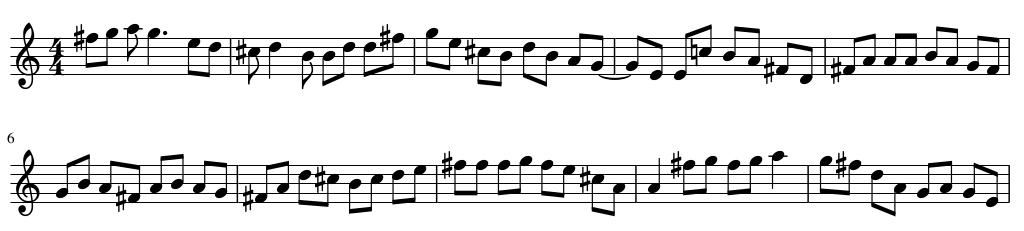
\includegraphics[scale=0.3]{images/chapter9/note_rnn_result.png}
\caption{Mélodie générée par le réseau \textit{note-rnn}.}
\label{result_note_rnn}
\end{center}
\end{figure}

La structure de la mélodie correspond à celle d'une gigue. Les hauteurs des notes qui se suivent sont souvent proches. Néanmoins, à l'écoute, le résultat n'est pas d'une grande qualité car il manque la basse qui est un élément essentiel pour une gigue. Dans les sections suivantes, nous allons étudier les solutions que nous avons proposées afin de générer des notes pour plusieurs instruments.

\subsection{Génération de notes pour plusieurs instruments en série}

La première idée pour étendre le réseau précédent à la génération de notes pour plusieurs instruments est de générer les notes en série. C'est-à-dire que le réseau génère les notes une par une en choisissant pour quel instrument il génère la note à chaque fois.

\subsubsection{Architecture}

Une note sera maintenant modélisée par un instrument, une hauteur et une durée. On associe alors à une note un vecteur de $\mathbb{R}^{l+m+n}$ où :
\begin{itemize}
\item les $l$ premières dimensions servent à spécifier l'instrument qui joue la note ;
\item les $m$ suivantes servent à décrire la hauteur de la note ou un caractère spécial (silence, début d'un morceau, ...) ;
\item les $n$ dernières la durée de la note.
\end{itemize}

On retrouvera l'architecture du réseau sur la figure \label{series_rnn}. On utilise ici trois fois la fonction $softmax$ en sortie afin de générer trois distributions de probabilités : une pour l'instrument, une pour la hauteur et une pour la durée. On utilise alors une fonction de coût idoine qui est la somme de trois $softmaxCE$. 

\begin{figure}[h!]
\begin{center}
% Graphic for TeX using PGF
% Title: /home/pierre/Programming/pl-lstm/images/illustrations_cr/series_rnn.dia
% Creator: Dia v0.97.3
% CreationDate: Tue Jun 13 13:32:35 2017
% For: pierre
% \usepackage{tikz}
% The following commands are not supported in PSTricks at present
% We define them conditionally, so when they are implemented,
% this pgf file will use them.
\ifx\du\undefined
  \newlength{\du}
\fi
\setlength{\du}{15\unitlength}
\begin{tikzpicture}[scale=0.85]
\pgftransformxscale{1.000000}
\pgftransformyscale{-1.000000}
\definecolor{dialinecolor}{rgb}{0.000000, 0.000000, 0.000000}
\pgfsetstrokecolor{dialinecolor}
\definecolor{dialinecolor}{rgb}{1.000000, 1.000000, 1.000000}
\pgfsetfillcolor{dialinecolor}
\pgfsetlinewidth{0.100000\du}
\pgfsetdash{}{0pt}
\pgfsetdash{}{0pt}
\pgfsetroundjoin
{\pgfsetcornersarced{\pgfpoint{1.000000\du}{1.000000\du}}\definecolor{dialinecolor}{rgb}{0.882353, 0.968627, 0.815686}
\pgfsetfillcolor{dialinecolor}
\fill (10.000000\du,12.000000\du)--(10.000000\du,20.000000\du)--(24.000000\du,20.000000\du)--(24.000000\du,12.000000\du)--cycle;
}{\pgfsetcornersarced{\pgfpoint{1.000000\du}{1.000000\du}}\definecolor{dialinecolor}{rgb}{0.427451, 0.529412, 0.349020}
\pgfsetstrokecolor{dialinecolor}
\draw (10.000000\du,12.000000\du)--(10.000000\du,20.000000\du)--(24.000000\du,20.000000\du)--(24.000000\du,12.000000\du)--cycle;
}\pgfsetlinewidth{0.100000\du}
\pgfsetdash{}{0pt}
\pgfsetdash{}{0pt}
\pgfsetbuttcap
{
\definecolor{dialinecolor}{rgb}{0.000000, 0.000000, 0.000000}
\pgfsetfillcolor{dialinecolor}
% was here!!!
\pgfsetarrowsend{latex}
\definecolor{dialinecolor}{rgb}{0.000000, 0.000000, 0.000000}
\pgfsetstrokecolor{dialinecolor}
\draw (21.000000\du,12.000000\du)--(21.000000\du,10.000000\du);
}
\pgfsetlinewidth{0.100000\du}
\pgfsetdash{}{0pt}
\pgfsetdash{}{0pt}
\pgfsetbuttcap
{
\definecolor{dialinecolor}{rgb}{0.000000, 0.000000, 0.000000}
\pgfsetfillcolor{dialinecolor}
% was here!!!
\pgfsetarrowsend{latex}
\definecolor{dialinecolor}{rgb}{0.000000, 0.000000, 0.000000}
\pgfsetstrokecolor{dialinecolor}
\draw (24.000000\du,16.000000\du)--(28.000000\du,16.000000\du);
}
% setfont left to latex
\definecolor{dialinecolor}{rgb}{0.000000, 0.000000, 0.000000}
\pgfsetstrokecolor{dialinecolor}
\node at (8.000000\du,15.293750\du){$H(t-1)$};
\pgfsetlinewidth{0.100000\du}
\pgfsetdash{}{0pt}
\pgfsetdash{}{0pt}
\pgfsetbuttcap
{
\definecolor{dialinecolor}{rgb}{0.000000, 0.000000, 0.000000}
\pgfsetfillcolor{dialinecolor}
% was here!!!
\pgfsetarrowsend{latex}
\definecolor{dialinecolor}{rgb}{0.000000, 0.000000, 0.000000}
\pgfsetstrokecolor{dialinecolor}
\draw (12.000000\du,22.000000\du)--(12.000000\du,20.000000\du);
}
% setfont left to latex
\definecolor{dialinecolor}{rgb}{0.000000, 0.000000, 0.000000}
\pgfsetstrokecolor{dialinecolor}
\node at (26.000000\du,15.293750\du){$H(t)$};
% setfont left to latex
\definecolor{dialinecolor}{rgb}{0.000000, 0.000000, 0.000000}
\pgfsetstrokecolor{dialinecolor}
\node at (14.000000\du,21.293750\du){$X(t)$};
% setfont left to latex
\definecolor{dialinecolor}{rgb}{0.000000, 0.000000, 0.000000}
\pgfsetstrokecolor{dialinecolor}
\node at (17.000000\du,16.391250\du){LSTMs};
\pgfsetlinewidth{0.100000\du}
\pgfsetdash{}{0pt}
\pgfsetdash{}{0pt}
\pgfsetbuttcap
{
\definecolor{dialinecolor}{rgb}{0.000000, 0.000000, 0.000000}
\pgfsetfillcolor{dialinecolor}
% was here!!!
\pgfsetarrowsend{latex}
\definecolor{dialinecolor}{rgb}{0.000000, 0.000000, 0.000000}
\pgfsetstrokecolor{dialinecolor}
\draw (6.000000\du,16.000000\du)--(10.000000\du,16.000000\du);
}
% setfont left to latex
\definecolor{dialinecolor}{rgb}{0.000000, 0.000000, 0.000000}
\pgfsetstrokecolor{dialinecolor}
\node at (23.000000\du,11.293750\du){$Y(t)$};
\pgfsetlinewidth{0.100000\du}
\pgfsetdash{}{0pt}
\pgfsetdash{}{0pt}
\pgfsetmiterjoin
\definecolor{dialinecolor}{rgb}{0.960784, 0.933333, 0.611765}
\pgfsetfillcolor{dialinecolor}
\fill (4.500000\du,22.000000\du)--(4.500000\du,24.000000\du)--(10.500000\du,24.000000\du)--(10.500000\du,22.000000\du)--cycle;
\definecolor{dialinecolor}{rgb}{0.000000, 0.000000, 0.000000}
\pgfsetstrokecolor{dialinecolor}
\draw (4.500000\du,22.000000\du)--(4.500000\du,24.000000\du)--(10.500000\du,24.000000\du)--(10.500000\du,22.000000\du)--cycle;
\pgfsetlinewidth{0.100000\du}
\pgfsetdash{}{0pt}
\pgfsetdash{}{0pt}
\pgfsetmiterjoin
\definecolor{dialinecolor}{rgb}{0.960784, 0.933333, 0.611765}
\pgfsetfillcolor{dialinecolor}
\fill (10.500000\du,22.000000\du)--(10.500000\du,24.000000\du)--(15.500000\du,24.000000\du)--(15.500000\du,22.000000\du)--cycle;
\definecolor{dialinecolor}{rgb}{0.000000, 0.000000, 0.000000}
\pgfsetstrokecolor{dialinecolor}
\draw (10.500000\du,22.000000\du)--(10.500000\du,24.000000\du)--(15.500000\du,24.000000\du)--(15.500000\du,22.000000\du)--cycle;
\pgfsetlinewidth{0.100000\du}
\pgfsetdash{}{0pt}
\pgfsetdash{}{0pt}
\pgfsetmiterjoin
\definecolor{dialinecolor}{rgb}{0.960784, 0.933333, 0.611765}
\pgfsetfillcolor{dialinecolor}
\fill (15.500000\du,22.000000\du)--(15.500000\du,24.000000\du)--(19.500000\du,24.000000\du)--(19.500000\du,22.000000\du)--cycle;
\definecolor{dialinecolor}{rgb}{0.000000, 0.000000, 0.000000}
\pgfsetstrokecolor{dialinecolor}
\draw (15.500000\du,22.000000\du)--(15.500000\du,24.000000\du)--(19.500000\du,24.000000\du)--(19.500000\du,22.000000\du)--cycle;
% setfont left to latex
\definecolor{dialinecolor}{rgb}{0.000000, 0.000000, 0.000000}
\pgfsetstrokecolor{dialinecolor}
\node at (7.500000\du,23.222500\du){Instrument(t)};
% setfont left to latex
\definecolor{dialinecolor}{rgb}{0.000000, 0.000000, 0.000000}
\pgfsetstrokecolor{dialinecolor}
\node at (13.000000\du,23.222500\du){Hauteur(t)};
% setfont left to latex
\definecolor{dialinecolor}{rgb}{0.000000, 0.000000, 0.000000}
\pgfsetstrokecolor{dialinecolor}
\node at (17.500000\du,23.222500\du){Durée(t)};
\pgfsetlinewidth{0.100000\du}
\pgfsetdash{}{0pt}
\pgfsetdash{}{0pt}
\pgfsetmiterjoin
\definecolor{dialinecolor}{rgb}{0.960784, 0.933333, 0.611765}
\pgfsetfillcolor{dialinecolor}
\fill (13.500000\du,8.000000\du)--(13.500000\du,10.000000\du)--(19.500000\du,10.000000\du)--(19.500000\du,8.000000\du)--cycle;
\definecolor{dialinecolor}{rgb}{0.000000, 0.000000, 0.000000}
\pgfsetstrokecolor{dialinecolor}
\draw (13.500000\du,8.000000\du)--(13.500000\du,10.000000\du)--(19.500000\du,10.000000\du)--(19.500000\du,8.000000\du)--cycle;
\pgfsetlinewidth{0.100000\du}
\pgfsetdash{}{0pt}
\pgfsetdash{}{0pt}
\pgfsetmiterjoin
\definecolor{dialinecolor}{rgb}{0.960784, 0.933333, 0.611765}
\pgfsetfillcolor{dialinecolor}
\fill (19.500000\du,8.000000\du)--(19.500000\du,10.000000\du)--(24.500000\du,10.000000\du)--(24.500000\du,8.000000\du)--cycle;
\definecolor{dialinecolor}{rgb}{0.000000, 0.000000, 0.000000}
\pgfsetstrokecolor{dialinecolor}
\draw (19.500000\du,8.000000\du)--(19.500000\du,10.000000\du)--(24.500000\du,10.000000\du)--(24.500000\du,8.000000\du)--cycle;
\pgfsetlinewidth{0.100000\du}
\pgfsetdash{}{0pt}
\pgfsetdash{}{0pt}
\pgfsetmiterjoin
\definecolor{dialinecolor}{rgb}{0.960784, 0.933333, 0.611765}
\pgfsetfillcolor{dialinecolor}
\fill (24.500000\du,8.000000\du)--(24.500000\du,10.000000\du)--(28.500000\du,10.000000\du)--(28.500000\du,8.000000\du)--cycle;
\definecolor{dialinecolor}{rgb}{0.000000, 0.000000, 0.000000}
\pgfsetstrokecolor{dialinecolor}
\draw (24.500000\du,8.000000\du)--(24.500000\du,10.000000\du)--(28.500000\du,10.000000\du)--(28.500000\du,8.000000\du)--cycle;
% setfont left to latex
\definecolor{dialinecolor}{rgb}{0.000000, 0.000000, 0.000000}
\pgfsetstrokecolor{dialinecolor}
\node at (16.500000\du,9.222500\du){Instrument(t+1)};
% setfont left to latex
\definecolor{dialinecolor}{rgb}{0.000000, 0.000000, 0.000000}
\pgfsetstrokecolor{dialinecolor}
\node at (22.000000\du,9.222500\du){Hauteur(t+1)};
% setfont left to latex
\definecolor{dialinecolor}{rgb}{0.000000, 0.000000, 0.000000}
\pgfsetstrokecolor{dialinecolor}
\node at (26.500000\du,9.222500\du){Durée(t+1)};
\end{tikzpicture}

\caption{Architecture du réseau utilisé pour la génération de notes pour plusieurs instruments en série.}
\label{series_rnn}
\end{center}
\end{figure}

\subsubsection{Résultats}

Les résultats sont obtenus après entrainement sur l'ensemble de gigues en séparant les notes des deux instruments.

On retrouvera un exemple de partition générée par cette architecture.

\begin{figure}[h!]
\begin{center}
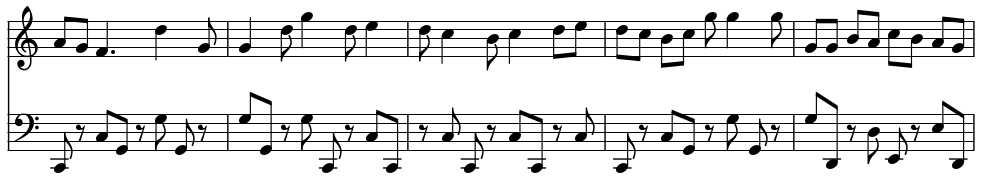
\includegraphics[scale=0.3]{images/chapter9/series_rnn_result.png}
\caption{Partition générée par le réseau \textit{series-rnn}.}
\end{center}
\end{figure}

On remarque que le réseau arrive bien à générer une mélodie et une basse. Les morceaux de musique ainsi générés sont d'assez bonne facture. Néanmoins, un des problèmes majeurs de cette architecture est que ce soit le réseau qui choisit l'instrument qui joue des notes à chaque pas de temps. Il peut avoir tendance à générer plus de notes pour un instrument qu'un autre.

Cette architecture peut très facilement s'étendre à plus de deux instruments.

\subsection{Génération de notes pour plusieurs instruments en parallèle}

Finalement la dernière architecture que nous avons considérée est la génération de notes en parallèle pour plusieurs instruments ce qui permet d'éviter que le réseau génère plus de notes pour un instrument qu'un autre.

Au début, nous voulions qu'à chaque pas de temps le réseau génère une note pour chaque instrument. Cependant cette méthodologie a un grand problème qui est dû au fait que les notes peuvent avoir des durées très différentes. Ainsi même si chaque instrument aurait eu le même nombre de notes, leur partition respective auraient pu avoir des durées très différentes.

Afin de remédier à ce problème, nous avons fait le constat que l'unité de temps constante pour tous les instruments est la mesure. Notre idée est donc de générer en parallèle une mesure pour chaque instrument à chaque pas de temps du réseau.

Le problème réside donc maintenant dans la représentation des mesures pour les mettre en entrée d'un réseau de neurones. En effet, les mesures peuvent contenir un nombre de notes très variable, il n'est donc pas évident de créer un encodage de taille fixe pour celles-ci. La solution que nous avons choisie est d'utiliser un réseau de neurones spécial, un autoencodeur, pour réaliser l'encodage et le décodage des mesures.

\subsubsection{Autoencodeur de mesures}

Un autoencodeur est un réseau qui prend une entrée, fournit une représentation intermédiaire puis essaye de prédire son entrée grâce à cette représentation intermédiaire.

Souvent on utilise des autoencodeurs afin de faire de la compression ou de la réduction de dimension en choisissant une représentation intermédiaire de taille inférieure à la taille de l'entrée.

Dans notre cas, nous utilisons des autoencodeurs afin de créer une représentation de taille fixe pour les séquences de notes de taille variable que sont les mesures.

Sur la figure \ref{autoencoder} se trouve l'architecture que nous avons utilisé pour notre autoencodeur. Le réseau peut se décomposer en deux parties l'encodeur et le décodeur. La représentation intermédiaire que nous utilisons est le vecteur $c$, sa taille est déterminée par la taille de l'état caché des cellules LSTM de l'encodeur. Lors de l'apprentissage, le réseau est entrainé comme une seule et unique partie. Cependant lors de la génération de mesures, nous allons d'abord utiliser seulement la partie encodeur pour encoder les mesures afin de les mettre en entrée du réseau. Puis, nous utiliserons seulement la partie décodeur afin de décoder les sorties du réseau. 

\begin{figure}[h!]
\begin{center}
% Graphic for TeX using PGF
% Title: /home/pierre/Programming/pl-lstm/images/illustrations_cr/autoencoder.dia
% Creator: Dia v0.97.3
% CreationDate: Tue Jun 13 13:41:25 2017
% For: pierre
% \usepackage{tikz}
% The following commands are not supported in PSTricks at present
% We define them conditionally, so when they are implemented,
% this pgf file will use them.
\ifx\du\undefined
  \newlength{\du}
\fi
\setlength{\du}{15\unitlength}
\begin{tikzpicture}[scale=0.7]
\pgftransformxscale{1.000000}
\pgftransformyscale{-1.000000}
\definecolor{dialinecolor}{rgb}{0.000000, 0.000000, 0.000000}
\pgfsetstrokecolor{dialinecolor}
\definecolor{dialinecolor}{rgb}{1.000000, 1.000000, 1.000000}
\pgfsetfillcolor{dialinecolor}
\pgfsetlinewidth{0.050000\du}
\pgfsetdash{{1.000000\du}{1.000000\du}}{0\du}
\pgfsetdash{{0.500000\du}{0.500000\du}}{0\du}
\pgfsetmiterjoin
\definecolor{dialinecolor}{rgb}{1.000000, 1.000000, 1.000000}
\pgfsetfillcolor{dialinecolor}
\fill (11.800000\du,5.800000\du)--(11.800000\du,9.200000\du)--(37.200000\du,9.200000\du)--(37.200000\du,5.800000\du)--cycle;
\definecolor{dialinecolor}{rgb}{0.000000, 0.000000, 0.000000}
\pgfsetstrokecolor{dialinecolor}
\draw (11.800000\du,5.800000\du)--(11.800000\du,9.200000\du)--(37.200000\du,9.200000\du)--(37.200000\du,5.800000\du)--cycle;
\pgfsetlinewidth{0.050000\du}
\pgfsetdash{{0.500000\du}{0.500000\du}}{0\du}
\pgfsetdash{{0.500000\du}{0.500000\du}}{0\du}
\pgfsetmiterjoin
\definecolor{dialinecolor}{rgb}{1.000000, 1.000000, 1.000000}
\pgfsetfillcolor{dialinecolor}
\fill (11.800000\du,12.800000\du)--(11.800000\du,15.800000\du)--(37.200000\du,15.800000\du)--(37.200000\du,12.800000\du)--cycle;
\definecolor{dialinecolor}{rgb}{0.000000, 0.000000, 0.000000}
\pgfsetstrokecolor{dialinecolor}
\draw (11.800000\du,12.800000\du)--(11.800000\du,15.800000\du)--(37.200000\du,15.800000\du)--(37.200000\du,12.800000\du)--cycle;
\pgfsetlinewidth{0.050000\du}
\pgfsetdash{}{0pt}
\pgfsetdash{}{0pt}
\pgfsetmiterjoin
\definecolor{dialinecolor}{rgb}{1.000000, 1.000000, 1.000000}
\pgfsetfillcolor{dialinecolor}
\fill (12.000000\du,13.000000\du)--(12.000000\du,15.000000\du)--(15.000000\du,15.000000\du)--(15.000000\du,13.000000\du)--cycle;
\definecolor{dialinecolor}{rgb}{0.000000, 0.000000, 0.000000}
\pgfsetstrokecolor{dialinecolor}
\draw (12.000000\du,13.000000\du)--(12.000000\du,15.000000\du)--(15.000000\du,15.000000\du)--(15.000000\du,13.000000\du)--cycle;
\pgfsetlinewidth{0.050000\du}
\pgfsetdash{}{0pt}
\pgfsetdash{}{0pt}
\pgfsetmiterjoin
\definecolor{dialinecolor}{rgb}{1.000000, 1.000000, 1.000000}
\pgfsetfillcolor{dialinecolor}
\fill (17.000000\du,13.000000\du)--(17.000000\du,15.000000\du)--(20.000000\du,15.000000\du)--(20.000000\du,13.000000\du)--cycle;
\definecolor{dialinecolor}{rgb}{0.000000, 0.000000, 0.000000}
\pgfsetstrokecolor{dialinecolor}
\draw (17.000000\du,13.000000\du)--(17.000000\du,15.000000\du)--(20.000000\du,15.000000\du)--(20.000000\du,13.000000\du)--cycle;
\pgfsetlinewidth{0.050000\du}
\pgfsetdash{}{0pt}
\pgfsetdash{}{0pt}
\pgfsetmiterjoin
\definecolor{dialinecolor}{rgb}{1.000000, 1.000000, 1.000000}
\pgfsetfillcolor{dialinecolor}
\fill (27.000000\du,13.000000\du)--(27.000000\du,15.000000\du)--(30.000000\du,15.000000\du)--(30.000000\du,13.000000\du)--cycle;
\definecolor{dialinecolor}{rgb}{0.000000, 0.000000, 0.000000}
\pgfsetstrokecolor{dialinecolor}
\draw (27.000000\du,13.000000\du)--(27.000000\du,15.000000\du)--(30.000000\du,15.000000\du)--(30.000000\du,13.000000\du)--cycle;
\pgfsetlinewidth{0.050000\du}
\pgfsetdash{}{0pt}
\pgfsetdash{}{0pt}
\pgfsetmiterjoin
\definecolor{dialinecolor}{rgb}{1.000000, 1.000000, 1.000000}
\pgfsetfillcolor{dialinecolor}
\fill (32.000000\du,13.000000\du)--(32.000000\du,15.000000\du)--(35.000000\du,15.000000\du)--(35.000000\du,13.000000\du)--cycle;
\definecolor{dialinecolor}{rgb}{0.000000, 0.000000, 0.000000}
\pgfsetstrokecolor{dialinecolor}
\draw (32.000000\du,13.000000\du)--(32.000000\du,15.000000\du)--(35.000000\du,15.000000\du)--(35.000000\du,13.000000\du)--cycle;
\pgfsetlinewidth{0.050000\du}
\pgfsetdash{}{0pt}
\pgfsetdash{}{0pt}
\pgfsetmiterjoin
\pgfsetbuttcap
{
\definecolor{dialinecolor}{rgb}{0.000000, 0.000000, 0.000000}
\pgfsetfillcolor{dialinecolor}
% was here!!!
\pgfsetarrowsend{latex}
{\pgfsetcornersarced{\pgfpoint{0.000000\du}{0.000000\du}}\definecolor{dialinecolor}{rgb}{0.000000, 0.000000, 0.000000}
\pgfsetstrokecolor{dialinecolor}
\draw (37.000000\du,10.000000\du)--(37.000000\du,9.000000\du)--(34.000000\du,9.000000\du)--(34.000000\du,8.000000\du);
}}
\pgfsetlinewidth{0.050000\du}
\pgfsetdash{}{0pt}
\pgfsetdash{}{0pt}
\pgfsetmiterjoin
\definecolor{dialinecolor}{rgb}{1.000000, 1.000000, 1.000000}
\pgfsetfillcolor{dialinecolor}
\fill (12.000000\du,6.000000\du)--(12.000000\du,8.000000\du)--(15.000000\du,8.000000\du)--(15.000000\du,6.000000\du)--cycle;
\definecolor{dialinecolor}{rgb}{0.000000, 0.000000, 0.000000}
\pgfsetstrokecolor{dialinecolor}
\draw (12.000000\du,6.000000\du)--(12.000000\du,8.000000\du)--(15.000000\du,8.000000\du)--(15.000000\du,6.000000\du)--cycle;
\pgfsetlinewidth{0.050000\du}
\pgfsetdash{}{0pt}
\pgfsetdash{}{0pt}
\pgfsetmiterjoin
\definecolor{dialinecolor}{rgb}{1.000000, 1.000000, 1.000000}
\pgfsetfillcolor{dialinecolor}
\fill (17.000000\du,6.000000\du)--(17.000000\du,8.000000\du)--(20.000000\du,8.000000\du)--(20.000000\du,6.000000\du)--cycle;
\definecolor{dialinecolor}{rgb}{0.000000, 0.000000, 0.000000}
\pgfsetstrokecolor{dialinecolor}
\draw (17.000000\du,6.000000\du)--(17.000000\du,8.000000\du)--(20.000000\du,8.000000\du)--(20.000000\du,6.000000\du)--cycle;
\pgfsetlinewidth{0.050000\du}
\pgfsetdash{}{0pt}
\pgfsetdash{}{0pt}
\pgfsetmiterjoin
\definecolor{dialinecolor}{rgb}{1.000000, 1.000000, 1.000000}
\pgfsetfillcolor{dialinecolor}
\fill (27.000000\du,6.000000\du)--(27.000000\du,8.000000\du)--(30.000000\du,8.000000\du)--(30.000000\du,6.000000\du)--cycle;
\definecolor{dialinecolor}{rgb}{0.000000, 0.000000, 0.000000}
\pgfsetstrokecolor{dialinecolor}
\draw (27.000000\du,6.000000\du)--(27.000000\du,8.000000\du)--(30.000000\du,8.000000\du)--(30.000000\du,6.000000\du)--cycle;
\pgfsetlinewidth{0.050000\du}
\pgfsetdash{}{0pt}
\pgfsetdash{}{0pt}
\pgfsetmiterjoin
\definecolor{dialinecolor}{rgb}{1.000000, 1.000000, 1.000000}
\pgfsetfillcolor{dialinecolor}
\fill (32.000000\du,6.000000\du)--(32.000000\du,8.000000\du)--(35.000000\du,8.000000\du)--(35.000000\du,6.000000\du)--cycle;
\definecolor{dialinecolor}{rgb}{0.000000, 0.000000, 0.000000}
\pgfsetstrokecolor{dialinecolor}
\draw (32.000000\du,6.000000\du)--(32.000000\du,8.000000\du)--(35.000000\du,8.000000\du)--(35.000000\du,6.000000\du)--cycle;
\pgfsetlinewidth{0.050000\du}
\pgfsetdash{}{0pt}
\pgfsetdash{}{0pt}
\pgfsetbuttcap
{
\definecolor{dialinecolor}{rgb}{0.000000, 0.000000, 0.000000}
\pgfsetfillcolor{dialinecolor}
% was here!!!
\pgfsetarrowsend{latex}
\definecolor{dialinecolor}{rgb}{0.000000, 0.000000, 0.000000}
\pgfsetstrokecolor{dialinecolor}
\draw (13.000000\du,16.000000\du)--(13.000000\du,15.000000\du);
}
\pgfsetlinewidth{0.050000\du}
\pgfsetdash{}{0pt}
\pgfsetdash{}{0pt}
\pgfsetbuttcap
{
\definecolor{dialinecolor}{rgb}{0.000000, 0.000000, 0.000000}
\pgfsetfillcolor{dialinecolor}
% was here!!!
\pgfsetarrowsend{latex}
\definecolor{dialinecolor}{rgb}{0.000000, 0.000000, 0.000000}
\pgfsetstrokecolor{dialinecolor}
\draw (18.000000\du,16.000000\du)--(18.000000\du,15.000000\du);
}
\pgfsetlinewidth{0.050000\du}
\pgfsetdash{}{0pt}
\pgfsetdash{}{0pt}
\pgfsetbuttcap
{
\definecolor{dialinecolor}{rgb}{0.000000, 0.000000, 0.000000}
\pgfsetfillcolor{dialinecolor}
% was here!!!
\pgfsetarrowsend{latex}
\definecolor{dialinecolor}{rgb}{0.000000, 0.000000, 0.000000}
\pgfsetstrokecolor{dialinecolor}
\draw (28.000000\du,16.000000\du)--(28.000000\du,15.000000\du);
}
\pgfsetlinewidth{0.050000\du}
\pgfsetdash{}{0pt}
\pgfsetdash{}{0pt}
\pgfsetbuttcap
{
\definecolor{dialinecolor}{rgb}{0.000000, 0.000000, 0.000000}
\pgfsetfillcolor{dialinecolor}
% was here!!!
\pgfsetarrowsend{latex}
\definecolor{dialinecolor}{rgb}{0.000000, 0.000000, 0.000000}
\pgfsetstrokecolor{dialinecolor}
\draw (33.000000\du,16.000000\du)--(33.000000\du,15.000000\du);
}
\pgfsetlinewidth{0.050000\du}
\pgfsetdash{}{0pt}
\pgfsetdash{}{0pt}
\pgfsetbuttcap
{
\definecolor{dialinecolor}{rgb}{0.000000, 0.000000, 0.000000}
\pgfsetfillcolor{dialinecolor}
% was here!!!
\pgfsetarrowsend{latex}
\definecolor{dialinecolor}{rgb}{0.000000, 0.000000, 0.000000}
\pgfsetstrokecolor{dialinecolor}
\draw (32.000000\du,7.000000\du)--(30.000000\du,7.000000\du);
}
\pgfsetlinewidth{0.050000\du}
\pgfsetdash{}{0pt}
\pgfsetdash{}{0pt}
\pgfsetbuttcap
{
\definecolor{dialinecolor}{rgb}{0.000000, 0.000000, 0.000000}
\pgfsetfillcolor{dialinecolor}
% was here!!!
\pgfsetarrowsend{latex}
\definecolor{dialinecolor}{rgb}{0.000000, 0.000000, 0.000000}
\pgfsetstrokecolor{dialinecolor}
\draw (27.000000\du,7.000000\du)--(25.000000\du,7.000000\du);
}
\pgfsetlinewidth{0.050000\du}
\pgfsetdash{}{0pt}
\pgfsetdash{}{0pt}
\pgfsetbuttcap
{
\definecolor{dialinecolor}{rgb}{0.000000, 0.000000, 0.000000}
\pgfsetfillcolor{dialinecolor}
% was here!!!
\pgfsetarrowsend{latex}
\definecolor{dialinecolor}{rgb}{0.000000, 0.000000, 0.000000}
\pgfsetstrokecolor{dialinecolor}
\draw (17.000000\du,7.000000\du)--(15.000000\du,7.000000\du);
}
\pgfsetlinewidth{0.050000\du}
\pgfsetdash{}{0pt}
\pgfsetdash{}{0pt}
\pgfsetbuttcap
{
\definecolor{dialinecolor}{rgb}{0.000000, 0.000000, 0.000000}
\pgfsetfillcolor{dialinecolor}
% was here!!!
\pgfsetarrowsend{latex}
\definecolor{dialinecolor}{rgb}{0.000000, 0.000000, 0.000000}
\pgfsetstrokecolor{dialinecolor}
\draw (15.000000\du,14.000000\du)--(17.000000\du,14.000000\du);
}
\pgfsetlinewidth{0.050000\du}
\pgfsetdash{}{0pt}
\pgfsetdash{}{0pt}
\pgfsetbuttcap
{
\definecolor{dialinecolor}{rgb}{0.000000, 0.000000, 0.000000}
\pgfsetfillcolor{dialinecolor}
% was here!!!
\pgfsetarrowsend{latex}
\definecolor{dialinecolor}{rgb}{0.000000, 0.000000, 0.000000}
\pgfsetstrokecolor{dialinecolor}
\draw (20.000000\du,14.000000\du)--(22.000000\du,14.000000\du);
}
\pgfsetlinewidth{0.050000\du}
\pgfsetdash{}{0pt}
\pgfsetdash{}{0pt}
\pgfsetbuttcap
{
\definecolor{dialinecolor}{rgb}{0.000000, 0.000000, 0.000000}
\pgfsetfillcolor{dialinecolor}
% was here!!!
\pgfsetarrowsend{latex}
\definecolor{dialinecolor}{rgb}{0.000000, 0.000000, 0.000000}
\pgfsetstrokecolor{dialinecolor}
\draw (30.000000\du,14.000000\du)--(32.000000\du,14.000000\du);
}
% setfont left to latex
\definecolor{dialinecolor}{rgb}{0.000000, 0.000000, 0.000000}
\pgfsetstrokecolor{dialinecolor}
\node at (37.000000\du,11.293750\du){$c$};
% setfont left to latex
\definecolor{dialinecolor}{rgb}{0.000000, 0.000000, 0.000000}
\pgfsetstrokecolor{dialinecolor}
\node at (13.000000\du,17.293750\du){$x_1$};
\pgfsetlinewidth{0.050000\du}
\pgfsetdash{}{0pt}
\pgfsetdash{}{0pt}
\pgfsetbuttcap
{
\definecolor{dialinecolor}{rgb}{0.000000, 0.000000, 0.000000}
\pgfsetfillcolor{dialinecolor}
% was here!!!
\pgfsetarrowsend{latex}
\definecolor{dialinecolor}{rgb}{0.000000, 0.000000, 0.000000}
\pgfsetstrokecolor{dialinecolor}
\draw (25.000000\du,14.000000\du)--(27.000000\du,14.000000\du);
}
\pgfsetlinewidth{0.050000\du}
\pgfsetdash{}{0pt}
\pgfsetdash{}{0pt}
\pgfsetbuttcap
{
\definecolor{dialinecolor}{rgb}{0.000000, 0.000000, 0.000000}
\pgfsetfillcolor{dialinecolor}
% was here!!!
\pgfsetarrowsend{latex}
\definecolor{dialinecolor}{rgb}{0.000000, 0.000000, 0.000000}
\pgfsetstrokecolor{dialinecolor}
\draw (22.000000\du,7.000000\du)--(20.000000\du,7.000000\du);
}
% setfont left to latex
\definecolor{dialinecolor}{rgb}{0.000000, 0.000000, 0.000000}
\pgfsetstrokecolor{dialinecolor}
\node at (23.500000\du,7.293750\du){$...$};
% setfont left to latex
\definecolor{dialinecolor}{rgb}{0.000000, 0.000000, 0.000000}
\pgfsetstrokecolor{dialinecolor}
\node at (23.500000\du,14.293750\du){$...$};
% setfont left to latex
\definecolor{dialinecolor}{rgb}{0.000000, 0.000000, 0.000000}
\pgfsetstrokecolor{dialinecolor}
\node at (18.000000\du,17.293750\du){$x_2$};
% setfont left to latex
\definecolor{dialinecolor}{rgb}{0.000000, 0.000000, 0.000000}
\pgfsetstrokecolor{dialinecolor}
\node at (28.000000\du,17.293750\du){$x_M$};
% setfont left to latex
\definecolor{dialinecolor}{rgb}{0.000000, 0.000000, 0.000000}
\pgfsetstrokecolor{dialinecolor}
\node at (33.000000\du,17.293750\du){$<eos>$};
\pgfsetlinewidth{0.050000\du}
\pgfsetdash{}{0pt}
\pgfsetdash{}{0pt}
\pgfsetbuttcap
{
\definecolor{dialinecolor}{rgb}{0.000000, 0.000000, 0.000000}
\pgfsetfillcolor{dialinecolor}
% was here!!!
\pgfsetarrowsend{latex}
\definecolor{dialinecolor}{rgb}{0.000000, 0.000000, 0.000000}
\pgfsetstrokecolor{dialinecolor}
\draw (13.000000\du,6.000000\du)--(13.000000\du,5.000000\du);
}
\pgfsetlinewidth{0.050000\du}
\pgfsetdash{}{0pt}
\pgfsetdash{}{0pt}
\pgfsetbuttcap
{
\definecolor{dialinecolor}{rgb}{0.000000, 0.000000, 0.000000}
\pgfsetfillcolor{dialinecolor}
% was here!!!
\pgfsetarrowsend{latex}
\definecolor{dialinecolor}{rgb}{0.000000, 0.000000, 0.000000}
\pgfsetstrokecolor{dialinecolor}
\draw (18.000000\du,6.000000\du)--(18.000000\du,5.000000\du);
}
\pgfsetlinewidth{0.050000\du}
\pgfsetdash{}{0pt}
\pgfsetdash{}{0pt}
\pgfsetbuttcap
{
\definecolor{dialinecolor}{rgb}{0.000000, 0.000000, 0.000000}
\pgfsetfillcolor{dialinecolor}
% was here!!!
\pgfsetarrowsend{latex}
\definecolor{dialinecolor}{rgb}{0.000000, 0.000000, 0.000000}
\pgfsetstrokecolor{dialinecolor}
\draw (28.000000\du,6.000000\du)--(28.000000\du,5.000000\du);
}
\pgfsetlinewidth{0.050000\du}
\pgfsetdash{}{0pt}
\pgfsetdash{}{0pt}
\pgfsetbuttcap
{
\definecolor{dialinecolor}{rgb}{0.000000, 0.000000, 0.000000}
\pgfsetfillcolor{dialinecolor}
% was here!!!
\pgfsetarrowsend{latex}
\definecolor{dialinecolor}{rgb}{0.000000, 0.000000, 0.000000}
\pgfsetstrokecolor{dialinecolor}
\draw (33.000000\du,6.000000\du)--(33.000000\du,5.000000\du);
}
% setfont left to latex
\definecolor{dialinecolor}{rgb}{0.000000, 0.000000, 0.000000}
\pgfsetstrokecolor{dialinecolor}
\node at (13.000000\du,4.293750\du){$<eos>$};
% setfont left to latex
\definecolor{dialinecolor}{rgb}{0.000000, 0.000000, 0.000000}
\pgfsetstrokecolor{dialinecolor}
\node at (18.000000\du,4.293750\du){$\hat{x}_N$};
% setfont left to latex
\definecolor{dialinecolor}{rgb}{0.000000, 0.000000, 0.000000}
\pgfsetstrokecolor{dialinecolor}
\node at (28.000000\du,4.293750\du){$\hat{x}_2$};
% setfont left to latex
\definecolor{dialinecolor}{rgb}{0.000000, 0.000000, 0.000000}
\pgfsetstrokecolor{dialinecolor}
\node at (33.000000\du,4.293750\du){$\hat{x}_1$};
\pgfsetlinewidth{0.050000\du}
\pgfsetdash{}{0pt}
\pgfsetdash{}{0pt}
\pgfsetbuttcap
{
\definecolor{dialinecolor}{rgb}{0.000000, 0.000000, 0.000000}
\pgfsetfillcolor{dialinecolor}
% was here!!!
\pgfsetarrowsend{latex}
\definecolor{dialinecolor}{rgb}{0.000000, 0.000000, 0.000000}
\pgfsetstrokecolor{dialinecolor}
\draw (13.000000\du,9.000000\du)--(13.000000\du,8.000000\du);
}
\pgfsetlinewidth{0.050000\du}
\pgfsetdash{}{0pt}
\pgfsetdash{}{0pt}
\pgfsetbuttcap
{
\definecolor{dialinecolor}{rgb}{0.000000, 0.000000, 0.000000}
\pgfsetfillcolor{dialinecolor}
% was here!!!
\definecolor{dialinecolor}{rgb}{0.000000, 0.000000, 0.000000}
\pgfsetstrokecolor{dialinecolor}
\draw (13.000000\du,9.000000\du)--(34.000000\du,9.000000\du);
}
\pgfsetlinewidth{0.050000\du}
\pgfsetdash{}{0pt}
\pgfsetdash{}{0pt}
\pgfsetbuttcap
{
\definecolor{dialinecolor}{rgb}{0.000000, 0.000000, 0.000000}
\pgfsetfillcolor{dialinecolor}
% was here!!!
\pgfsetarrowsend{latex}
\definecolor{dialinecolor}{rgb}{0.000000, 0.000000, 0.000000}
\pgfsetstrokecolor{dialinecolor}
\draw (18.000000\du,9.000000\du)--(18.000000\du,8.000000\du);
}
\pgfsetlinewidth{0.050000\du}
\pgfsetdash{}{0pt}
\pgfsetdash{}{0pt}
\pgfsetbuttcap
{
\definecolor{dialinecolor}{rgb}{0.000000, 0.000000, 0.000000}
\pgfsetfillcolor{dialinecolor}
% was here!!!
\pgfsetarrowsend{latex}
\definecolor{dialinecolor}{rgb}{0.000000, 0.000000, 0.000000}
\pgfsetstrokecolor{dialinecolor}
\draw (28.000000\du,9.000000\du)--(28.000000\du,8.000000\du);
}
\pgfsetlinewidth{0.050000\du}
\pgfsetdash{}{0pt}
\pgfsetdash{}{0pt}
\pgfsetbuttcap
{
\definecolor{dialinecolor}{rgb}{0.000000, 0.000000, 0.000000}
\pgfsetfillcolor{dialinecolor}
% was here!!!
\definecolor{dialinecolor}{rgb}{0.000000, 0.000000, 0.000000}
\pgfsetstrokecolor{dialinecolor}
\draw (35.000000\du,14.000000\du)--(37.000000\du,14.000000\du);
}
\pgfsetlinewidth{0.050000\du}
\pgfsetdash{}{0pt}
\pgfsetdash{}{0pt}
\pgfsetbuttcap
{
\definecolor{dialinecolor}{rgb}{0.000000, 0.000000, 0.000000}
\pgfsetfillcolor{dialinecolor}
% was here!!!
\pgfsetarrowsend{latex}
\definecolor{dialinecolor}{rgb}{0.000000, 0.000000, 0.000000}
\pgfsetstrokecolor{dialinecolor}
\draw (37.000000\du,14.000000\du)--(37.000000\du,12.000000\du);
}
% setfont left to latex
\definecolor{dialinecolor}{rgb}{0.000000, 0.000000, 0.000000}
\pgfsetstrokecolor{dialinecolor}
\node at (9.000000\du,7.293750\du){Decodeur};
% setfont left to latex
\definecolor{dialinecolor}{rgb}{0.000000, 0.000000, 0.000000}
\pgfsetstrokecolor{dialinecolor}
\node at (9.000000\du,14.293750\du){Encodeur};
\end{tikzpicture}

\caption{Architecture d'un autoencodeur de séquences.}
\label{autoencoder}
\end{center}
\end{figure}

Après apprentissage sur les mesures de l'ensemble des gigues, en utilisant deux cellules LSTM à chaque pas de temps avec un état de taille $64$, le réseau a atteint une précision de $99.7\%$. C'est-à-dire que sur les $250000$ mesures de l'ensemble d'apprentissage que nous avons encodées puis décodées l'encodage, dans $99.7\%$ des cas, la mesure décodée était exactement la même que l'entrée.

\subsubsection{Architecture}

Maintenant que nous disposons d'un encodage de taille fixe pour les mesures, nous pouvons aisément créer une architecture de réseau générant des mesures. Sur la figure \ref{measure_rnn} se trouve l'architecture que nous avons utilisée.

En sortie du réseau, nous n'avons cette fois-ci pas utilisé la fonction $softmax$ afin de créer une distribution de probabilités car nous sommes dans un problème de régression : l'objectif de l'apprentissage est de générer un vecteur proche de celui de la mesure encodée en sortie. Ainsi, nous avons utilisé une fonction de coût quadratique.

\begin{figure}[h!]
\begin{center}
% Graphic for TeX using PGF
% Title: /home/pierre/Programming/pl-lstm/images/illustrations_cr/measure_rnn.dia
% Creator: Dia v0.97.3
% CreationDate: Tue Jun 13 13:44:52 2017
% For: pierre
% \usepackage{tikz}
% The following commands are not supported in PSTricks at present
% We define them conditionally, so when they are implemented,
% this pgf file will use them.
\ifx\du\undefined
  \newlength{\du}
\fi
\setlength{\du}{15\unitlength}
\begin{tikzpicture}[scale=0.85]
\pgftransformxscale{1.000000}
\pgftransformyscale{-1.000000}
\definecolor{dialinecolor}{rgb}{0.000000, 0.000000, 0.000000}
\pgfsetstrokecolor{dialinecolor}
\definecolor{dialinecolor}{rgb}{1.000000, 1.000000, 1.000000}
\pgfsetfillcolor{dialinecolor}
\pgfsetlinewidth{0.100000\du}
\pgfsetdash{}{0pt}
\pgfsetdash{}{0pt}
\pgfsetroundjoin
{\pgfsetcornersarced{\pgfpoint{1.000000\du}{1.000000\du}}\definecolor{dialinecolor}{rgb}{0.882353, 0.968627, 0.815686}
\pgfsetfillcolor{dialinecolor}
\fill (10.000000\du,12.000000\du)--(10.000000\du,20.000000\du)--(24.000000\du,20.000000\du)--(24.000000\du,12.000000\du)--cycle;
}{\pgfsetcornersarced{\pgfpoint{1.000000\du}{1.000000\du}}\definecolor{dialinecolor}{rgb}{0.427451, 0.529412, 0.349020}
\pgfsetstrokecolor{dialinecolor}
\draw (10.000000\du,12.000000\du)--(10.000000\du,20.000000\du)--(24.000000\du,20.000000\du)--(24.000000\du,12.000000\du)--cycle;
}\pgfsetlinewidth{0.100000\du}
\pgfsetdash{}{0pt}
\pgfsetdash{}{0pt}
\pgfsetbuttcap
{
\definecolor{dialinecolor}{rgb}{0.000000, 0.000000, 0.000000}
\pgfsetfillcolor{dialinecolor}
% was here!!!
\pgfsetarrowsend{latex}
\definecolor{dialinecolor}{rgb}{0.000000, 0.000000, 0.000000}
\pgfsetstrokecolor{dialinecolor}
\draw (21.000000\du,12.000000\du)--(21.000000\du,10.000000\du);
}
\pgfsetlinewidth{0.100000\du}
\pgfsetdash{}{0pt}
\pgfsetdash{}{0pt}
\pgfsetbuttcap
{
\definecolor{dialinecolor}{rgb}{0.000000, 0.000000, 0.000000}
\pgfsetfillcolor{dialinecolor}
% was here!!!
\pgfsetarrowsend{latex}
\definecolor{dialinecolor}{rgb}{0.000000, 0.000000, 0.000000}
\pgfsetstrokecolor{dialinecolor}
\draw (24.000000\du,16.000000\du)--(28.000000\du,16.000000\du);
}
% setfont left to latex
\definecolor{dialinecolor}{rgb}{0.000000, 0.000000, 0.000000}
\pgfsetstrokecolor{dialinecolor}
\node at (8.000000\du,15.293750\du){$H(t-1)$};
\pgfsetlinewidth{0.100000\du}
\pgfsetdash{}{0pt}
\pgfsetdash{}{0pt}
\pgfsetbuttcap
{
\definecolor{dialinecolor}{rgb}{0.000000, 0.000000, 0.000000}
\pgfsetfillcolor{dialinecolor}
% was here!!!
\pgfsetarrowsend{latex}
\definecolor{dialinecolor}{rgb}{0.000000, 0.000000, 0.000000}
\pgfsetstrokecolor{dialinecolor}
\draw (12.000000\du,22.000000\du)--(12.000000\du,20.000000\du);
}
% setfont left to latex
\definecolor{dialinecolor}{rgb}{0.000000, 0.000000, 0.000000}
\pgfsetstrokecolor{dialinecolor}
\node at (26.000000\du,15.293750\du){$H(t)$};
% setfont left to latex
\definecolor{dialinecolor}{rgb}{0.000000, 0.000000, 0.000000}
\pgfsetstrokecolor{dialinecolor}
\node at (14.000000\du,21.293750\du){$X(t)$};
% setfont left to latex
\definecolor{dialinecolor}{rgb}{0.000000, 0.000000, 0.000000}
\pgfsetstrokecolor{dialinecolor}
\node at (17.000000\du,16.391250\du){LSTMs};
\pgfsetlinewidth{0.100000\du}
\pgfsetdash{}{0pt}
\pgfsetdash{}{0pt}
\pgfsetbuttcap
{
\definecolor{dialinecolor}{rgb}{0.000000, 0.000000, 0.000000}
\pgfsetfillcolor{dialinecolor}
% was here!!!
\pgfsetarrowsend{latex}
\definecolor{dialinecolor}{rgb}{0.000000, 0.000000, 0.000000}
\pgfsetstrokecolor{dialinecolor}
\draw (6.000000\du,16.000000\du)--(10.000000\du,16.000000\du);
}
% setfont left to latex
\definecolor{dialinecolor}{rgb}{0.000000, 0.000000, 0.000000}
\pgfsetstrokecolor{dialinecolor}
\node at (23.000000\du,11.293750\du){$Y(t)$};
\pgfsetlinewidth{0.100000\du}
\pgfsetdash{}{0pt}
\pgfsetdash{}{0pt}
\pgfsetmiterjoin
\definecolor{dialinecolor}{rgb}{0.960784, 0.933333, 0.611765}
\pgfsetfillcolor{dialinecolor}
\fill (7.000000\du,22.000000\du)--(7.000000\du,24.000000\du)--(12.000000\du,24.000000\du)--(12.000000\du,22.000000\du)--cycle;
\definecolor{dialinecolor}{rgb}{0.000000, 0.000000, 0.000000}
\pgfsetstrokecolor{dialinecolor}
\draw (7.000000\du,22.000000\du)--(7.000000\du,24.000000\du)--(12.000000\du,24.000000\du)--(12.000000\du,22.000000\du)--cycle;
% setfont left to latex
\definecolor{dialinecolor}{rgb}{0.000000, 0.000000, 0.000000}
\pgfsetstrokecolor{dialinecolor}
\node at (9.500000\du,23.222500\du){Mesure1(t)};
\pgfsetlinewidth{0.100000\du}
\pgfsetdash{}{0pt}
\pgfsetdash{}{0pt}
\pgfsetmiterjoin
\definecolor{dialinecolor}{rgb}{0.960784, 0.933333, 0.611765}
\pgfsetfillcolor{dialinecolor}
\fill (12.000000\du,22.000000\du)--(12.000000\du,24.000000\du)--(17.000000\du,24.000000\du)--(17.000000\du,22.000000\du)--cycle;
\definecolor{dialinecolor}{rgb}{0.000000, 0.000000, 0.000000}
\pgfsetstrokecolor{dialinecolor}
\draw (12.000000\du,22.000000\du)--(12.000000\du,24.000000\du)--(17.000000\du,24.000000\du)--(17.000000\du,22.000000\du)--cycle;
% setfont left to latex
\definecolor{dialinecolor}{rgb}{0.000000, 0.000000, 0.000000}
\pgfsetstrokecolor{dialinecolor}
\node at (14.500000\du,23.222500\du){Mesure2(t)};
\pgfsetlinewidth{0.100000\du}
\pgfsetdash{}{0pt}
\pgfsetdash{}{0pt}
\pgfsetmiterjoin
\definecolor{dialinecolor}{rgb}{0.960784, 0.933333, 0.611765}
\pgfsetfillcolor{dialinecolor}
\fill (16.000000\du,8.000000\du)--(16.000000\du,10.000000\du)--(21.000000\du,10.000000\du)--(21.000000\du,8.000000\du)--cycle;
\definecolor{dialinecolor}{rgb}{0.000000, 0.000000, 0.000000}
\pgfsetstrokecolor{dialinecolor}
\draw (16.000000\du,8.000000\du)--(16.000000\du,10.000000\du)--(21.000000\du,10.000000\du)--(21.000000\du,8.000000\du)--cycle;
% setfont left to latex
\definecolor{dialinecolor}{rgb}{0.000000, 0.000000, 0.000000}
\pgfsetstrokecolor{dialinecolor}
\node at (18.500000\du,9.222500\du){Mesure1(t+1)};
\pgfsetlinewidth{0.100000\du}
\pgfsetdash{}{0pt}
\pgfsetdash{}{0pt}
\pgfsetmiterjoin
\definecolor{dialinecolor}{rgb}{0.960784, 0.933333, 0.611765}
\pgfsetfillcolor{dialinecolor}
\fill (21.000000\du,8.000000\du)--(21.000000\du,10.000000\du)--(26.000000\du,10.000000\du)--(26.000000\du,8.000000\du)--cycle;
\definecolor{dialinecolor}{rgb}{0.000000, 0.000000, 0.000000}
\pgfsetstrokecolor{dialinecolor}
\draw (21.000000\du,8.000000\du)--(21.000000\du,10.000000\du)--(26.000000\du,10.000000\du)--(26.000000\du,8.000000\du)--cycle;
% setfont left to latex
\definecolor{dialinecolor}{rgb}{0.000000, 0.000000, 0.000000}
\pgfsetstrokecolor{dialinecolor}
\node at (23.500000\du,9.222500\du){Mesure2(t+1)};
\end{tikzpicture}

\caption{Architecture du réseau utilisé pour la génération de notes pour plusieurs instruments en parallèle.}
\label{measure_rnn}
\end{center}
\end{figure}

Cette architecture s'étend très facilement à plus de deux instruments.

\subsubsection{Résultats}

On trouvera sur la figure \ref{result_measure_rnn}, une partition générée par l'architecture présentée.

\begin{figure}[h!]
\begin{center}
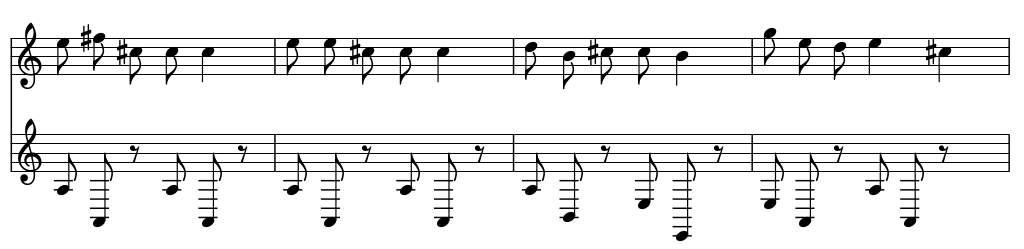
\includegraphics[scale=0.3]{images/chapter9/measure_rnn_result.png}
\caption{Partition générée par le réseau \textit{measure-rnn}.}
\label{result_measure_rnn}
\end{center}
\end{figure}

Les morceaux générés sont de très bonne qualité. À notre avis, ils sont d'une qualité supérieure à la génération série. Il serait intéressant de tester cette architecture sur des ensembles de musique comportant plus de deux instruments.

\subsection{Conclusion}

La génération de partitions a comme avantage de manipuler des données très quantifiées ce qui facilite grandement l'apprentissage et la qualité des morceaux générés.

Cependant, cette avantage est aussi une de ses faiblesses. En effet, il est plus difficile avec cette méthode de générer des musiques pour plusieurs instruments. Un point que nous n'avons d'ailleurs pas eu le temps de traiter est la génération d'accords c'est-à-dire de plusieurs notes en même temps pour plusieurs instruments. Nous pensons qu'il est possible de le faire en modifiant un peu nos architectures précédentes.

\section{Génération de signaux}
\subsection{Présentation du format}
Cette génération consiste à considérer la musique en tant que signal : cela nous permettra en effet de nous affranchir de la nécessité d'avoir un format de musique particulier et nous pourrons traiter directement des formats bien plus répandus comme le .mp3 ou le .wav. C'est précisément ce dernier que nous avons retenu, la librairie scipy de Python possédant des fonctions permettant d'appréhender très facilement ce format. L'entraînement se fera sur les coefficients de Fourier de ces signaux sonores, ceux-ci permettant de récupérer sous forme simple toute l'information relative aux morceaux.

\subsection{Principe}
La variété des morceaux .wav (durée, fréquence d'échantillonage...) et les contraintes matérielles (espace mémoire, temps de calcul...) nous ont poussé à devoir réaliser un prétraitement des données dans notre programme. Celui-ci sous échantillonne tout d'abord les morceaux à une fréquence $F_e = 16kHz$, la plupart des morceaux étant à $44kHz$ par défaut. Il s'agit ensuite de les découper en morceaux de durée T de l'ordre de la dizaine de millisecondes ($0,25$ dans notre implémentation). En effet, l'étape suivante consiste à appliquer la transformée de Fourier rapide sur chacun de ces morceaux élémentaires, il y aura donc $F_e \times T = 4000$ coefficients complexe au total, on voit donc tout l'intérêt du sous-échantillonage et du choix d'une durée T peu élevée. 

L'étape suivante est de séparer les contributions réelles et imaginaires de chaque coefficient, que l'on place alors dans des vecteurs de taille 8000. On possèdera finalement pour chaque morceau élémentaire un vecteur contenant ses coefficients de Fourier. Pour obtenir le morceau initial, il s'agira tout simplement de reformer les coefficients de Fourier avec leurs parties réelles et imaginaires, d'appliquer la transformée de Fourier rapide inverse et de concaténer les morceaux élémentaires.

Le réseau sera capable après entraînement de générer des morceaux de longueurs variables, décidée à l'avance par l'utilisateur, celle-ci étant simplement tributaire du nombre de vecteurs à générer.

\subsection{Résultat}

Le dataset est composé de morceaux de piano de durées variables. Le réseau est constitué de 2 cellules lstm avec un état caché de taille 512. L'algorithme d'optimisation utilisé est RMSProp, avec un learning rate de 0.95. Le coût, calculé avec la norme 2, décroît de plus de 1000 à 0.4 en 600 batchs. On soulignera l'importance de la normalisation des coefficients de Fourier pour éviter d'avoir des valeurs trop faibles lors du passage des valeurs dans les sigmoïdes.
La génération donne cependant un morceau très bruité dont la représentation spectrale est visible ci-dessous :

\begin{figure}[!h]
\begin{center}
	{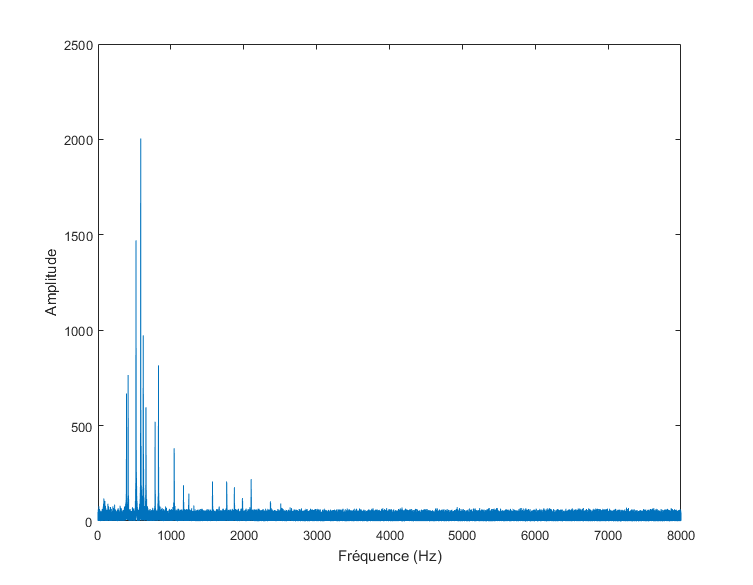
\includegraphics[scale=0.4]{images/chapter9/spectre.png}\label{spectre}}
  \caption{Représentation spectrale du morceau généré}
\end{center}
\end{figure}

Deux explications sont alors possibles. La première serait qu'il y a un problème dans le programme. La seconde consisterait à dire que le bruit est la structure la plus évidente à apprendre, étant présente en permanence. Nous avons été également limités par la taille de notre état caché : lorsque nous avons essayé de l'augmenter de façon significative, des erreurs mémoires ont été observées, la place occupée étant trop importante. Or plus l'état caché est de taille importante plus les cellules seront capables de saisir les spécificités des liens entre les différents instants. On peut donc raisonnablement penser que la limitation viendrait de là. Le manque de temps et de matériel nous a empêché de vérifier cette possibilité.




\nocite{*}

\bibliographystyle{plain}
\bibliography{compte-rendu.bib}

\end{document}
